\documentclass[a4paper,11pt,twoside]{memoir}
\chapterstyle{veelo}

\usepackage{TUINFDA}

\usepackage{hyperref}					% links in pdf
%\usepackage[pdfpagelabels]{hyperref}
\usepackage[all]{hypcap}			 % for going to the top of an image when a figure reference is clicked
\usepackage{cleveref}
\usepackage{listings}					% Provide listing environment
\usepackage{tabularx}					% Line breaks in tables
\usepackage{multirow}					% Multiple header tables
\usepackage{graphicx}         % Figures
\usepackage{verbatim}         % Code-Environment
\usepackage{amsmath}					% math environment
\usepackage{fixltx2e}					% provide subscripts
\usepackage{makecell}					% use table headers
\usepackage{fancyvrb}					% adjust verbatim environment
\usepackage{placeins}					% ensure images are contained in specific section
\usepackage{enumitem}					% reference enumerate items
\usepackage[lined,linesnumbered,algochapter]{algorithm2e} % Algorithm-Environment
%
%\usepackage{algpseudocode}
%\usepackage{algorithm}

\usepackage{ wasysym }				% package to display currency, e.g. cents

\usepackage{url}
\urlstyle{same}  % important for automatic line breaking in URLs

\usepackage{rotating}
\usepackage{lscape} % for rotating tables
\usepackage{lipsum}
\let\ab\allowbreak

\usepackage{pgf}					
\usepackage{tikz}					% tikz graphics
\usepackage{yfonts}				% additional typeset fonts
%\usepackage{boondox}			% additional typeset fonts
%\usepackage[cal=boondox,calscaled=.96]{mathalfa}
\usepackage[cal=pxtx,calscaled=.96]{mathalfa}
\usetikzlibrary{arrows,automata}

\usepackage{ngerman}
\usepackage[ngerman]{babel}
\usepackage{bibgerm,cite}       % Deutsche Bezeichnungen, Automatisches Zusammenfassen von Literaturstellen
\usepackage[ngerman]{varioref}  % Querverweise
% to use the german charset include cp850 for MS-DOS, ansinew for Windows and latin1 for Linux.
% \usepackage[latin1]{inputenc}

% allow page breaks within e.g. align environment
\allowdisplaybreaks

% settings for listing
\lstset{
  numbers=left, 
  firstnumber=1,
	breaklines=true,
  captionpos=b, 
	basicstyle=\footnotesize,
	numberstyle=\tiny\color{gray},
	frame=single,
  numberfirstline=true,
	aboveskip=2em
}

\thesistitle{Kosteneffizientes Ressourcenmanagement in verteilten Cloud Datenzentren}{Cost aware resource management in distributed cloud data centers}
\thesissubtitle{} % optional
\thesisdate{28.07.2015}

% all titles and designations have to be gender-related!
\thesisdegree{Diplom-Ingenieur}{Master of Science}
\thesiscurriculum{Informatik}{Computer Science} % your study
\thesisverfassung{Verfasser} % Verfasser
\thesisauthor{Andreas Egger} % your name
\thesisauthoraddress{Ospelgasse 35/3, 1200 Wien} % your address
\thesismatrikelno{0626885} % your registration number

\thesisbetreins{Priv.-Doz. Dr. Ivona Brandić}
\thesisbetrzwei{MSc. Dražen Lučanin}
\thesisbetrdrei{} % optional

% define page numbering styles
\makepagestyle{numberCorner}
\makeevenfoot{numberCorner}{\thepage}{}{}
\makeoddfoot{numberCorner}{}{}{\thepage}

% define custom macros for specific formats or names
\newcommand{\uml}[1]{\texttt{#1}}
\newcommand{\cd}{\textsf{Class Diagram}}

\begin{document}

\captionnamefont{\bfseries}

%%%%%%%%%%%%%%%%%%%%%%%%%%%%%%%%%%%%%%%%%
%%%   FRONTMATTER    %%%%%%%%%%%%%%%%%%%%
%%%%%%%%%%%%%%%%%%%%%%%%%%%%%%%%%%%%%%%%%
\frontmatter
\pagenumbering{roman}

%%%%%%%%%%%%%%%%%%%%%%%%%%%%%%%%%%%%%%%%%
%%%   TITLEPAGES    %%%%%%%%%%%%%%%%%%%%%
%%%%%%%%%%%%%%%%%%%%%%%%%%%%%%%%%%%%%%%%%

% the german title page is required as first page
% $Id: titlepage.tex 1752 2010-03-20 11:07:02Z tkren $
%
% TU Wien - Faculty of Informatics
% thesis titlepage
%
% This titlepage is using the geometry package, see
% <http://www.ctan.org/macros/latex/contrib/geometry/geometry.pdf>
%
% For questions and comments send an email to
% Thomas Krennwallner <tkren@kr.tuwien.ac.at>
% or to Petra Brosch <brosch@big.tuwien.ac.at>
%

\selectlanguage{ngerman}

% setup page dimensions for titlepage
\newgeometry{left=2.4cm,right=2.4cm,bottom=2.5cm,top=2cm}

% force baselineskip and parindent
\newlength{\tmpbaselineskip}
\setlength{\tmpbaselineskip}{\baselineskip}
\setlength{\baselineskip}{13.6pt}
\newlength{\tmpparindent}
\setlength{\tmpparindent}{\parindent}
\setlength{\parindent}{17pt}

% first titlepage
\thispagestyle{tuinftitlepage}

%
% Kludge: for each titlepage set \pagenumbering to a different
% style. This is used to fix a problem with hyperref, because there
% are multiple "page 1" and hyperref hates that
%
\pagenumbering{Alph}

\begin{center}
{\ \vspace{3.4cm}}

\begin{minipage}[t][2.8cm][s]{\textwidth}%
\centering
\thesistitlefontHUGE\sffamily\bfseries\tuinfthesistitle\\
\bigskip
{\thesistitlefonthuge\sffamily\bfseries\tuinfthesissubtitle}
\end{minipage}

\vspace{1.3cm}

{\thesistitlefontLARGE\sffamily \tuinfthesistype}

\vspace{6mm}

{\thesistitlefontlarge\sffamily zur Erlangung des akademischen Grades}

\vspace{6mm}

{\thesistitlefontLARGE\sffamily\bfseries \tuinfthesisdegree}

\vspace{6mm}

{\thesistitlefontlarge\sffamily im Rahmen des Studiums}

\vspace{6mm}

{\thesistitlefontLarge\sffamily\bfseries \tuinfthesiscurriculum}

\vspace{6.5mm}

{\thesistitlefontlarge\sffamily eingereicht von}

\vspace{6mm}

{\thesistitlefontLarge\sffamily\bfseries \tuinfthesisauthor}

\vspace{1.5mm}

{\thesistitlefontlarge\sffamily Matrikelnummer \tuinfthesismatrikelno} 

\vspace{1.4cm}

\vspace{0pt}\raggedright\thesistitlefontnormalsize\sffamily
\begin{minipage}[t][1.6cm][t]{\textwidth}%
  %
  an der

  Fakult\"{a}t f\"{u}r Informatik der Technischen Universit\"{a}t Wien
\end{minipage}

\begin{minipage}[t][4cm][t]{\textwidth}%
  \vspace{0pt}\raggedright\thesistitlefontnormalsize\sffamily
  %
  \begin{tabbing}%
	    \hspace{19mm} \= \hspace{66mm} \kill
	    \tuinfthesisbetreuung: \> \tuinfthesisbetreins\\
	    Mitwirkung: \> \tuinfthesisbetrzwei\\
	                \> \tuinfthesisbetrdrei
  \end{tabbing}
\end{minipage}

\begin{minipage}[t][1.5cm][t]{\textwidth}%
  \vspace{0pt}\sffamily\thesistitlefontnormalsize
  \begin{tabbing}%
    \hspace{45mm} \= \hspace{63mm} \= \hspace{51mm} \kill
    Wien, \tuinfthesisdate \> {\raggedright\rule{51mm}{0.5pt}} \> {\raggedright\rule{51mm}{0.5pt}} \\
    \> \begin{minipage}[t][0.5cm][t]{51mm}\centering (Unterschrift \tuinfthesisverfassung)\end{minipage}
    \> \begin{minipage}[t][0.5cm][t]{51mm}\centering (Unterschrift \tuinfthesisbetreuung)\end{minipage}
    \end{tabbing}
\end{minipage}

\end{center}

% we want an empty page right after first titlepage
\pagestyle{empty}
\cleardoublepage

% we're done with the titlepages, proceed with default pagenumbering
\pagenumbering{roman}

% restore baselineskip
\setlength{\baselineskip}{\tmpbaselineskip}
\setlength{\parindent}{\tmpparindent}

% back to normal geometry
\restoregeometry

\selectlanguage{english}

%%% Local Variables:
%%% TeX-PDF-mode: t
%%% TeX-debug-bad-boxes: t
%%% TeX-parse-self: t
%%% TeX-auto-save: t
%%% reftex-plug-into-AUCTeX: t
%%% End:


% an english translation may follow
% $Id: titlepage.tex 1752 2010-03-20 11:07:02Z tkren $
%
% TU Wien - Faculty of Informatics
% thesis titlepage
%
% This titlepage is using the geometry package, see
% <http://www.ctan.org/macros/latex/contrib/geometry/geometry.pdf>
%
% For questions and comments send an email to
% Thomas Krennwallner <tkren@kr.tuwien.ac.at>
% or to Petra Brosch <brosch@big.tuwien.ac.at>
%

% setup page dimensions for titlepage
\newgeometry{left=2.4cm,right=2.4cm,bottom=2.5cm,top=2cm}

% force baselineskip and parindent
%\newlength{\tmpbaselineskip}
%\setlength{\tmpbaselineskip}{\baselineskip}
%\setlength{\baselineskip}{13.6pt}
%\newlength{\tmpparindent}
%\setlength{\tmpparindent}{\parindent}
%\setlength{\parindent}{17pt}

% first titlepage
\thispagestyle{tuinftitlepage}

%
% Kludge: for each titlepage set \pagenumbering to a different
% style. This is used to fix a problem with hyperref, because there
% are multiple "page 1" and hyperref hates that
%
\pagenumbering{Roman}

\begin{center}
{\ \vspace{3.4cm}}

\begin{minipage}[t][2.8cm][s]{\textwidth}%
\centering
\thesistitlefontHUGE\sffamily\bfseries\tuinfthesistitle\\
\bigskip
{\thesistitlefonthuge\sffamily\bfseries\tuinfthesissubtitle}
\end{minipage}

\vspace{1.3cm}

{\thesistitlefontLARGE\sffamily \tuinfthesistypeen}

\vspace{6mm}

{\thesistitlefontlarge\sffamily submitted in partial fulfillment of the requirements for the degree of}

\vspace{6mm}

{\thesistitlefontLARGE\sffamily\bfseries \tuinfthesisdegreeen}

\vspace{6mm}

{\thesistitlefontlarge\sffamily in}

\vspace{6mm}

{\thesistitlefontLarge\sffamily\bfseries \tuinfthesiscurriculumen}

\vspace{6.5mm}

{\thesistitlefontlarge\sffamily by}

\vspace{6mm}

{\thesistitlefontLarge\sffamily\bfseries \tuinfthesisauthor}

\vspace{1.5mm}

{\thesistitlefontlarge\sffamily Registration Number \tuinfthesismatrikelno} 

\vspace{1.4cm}

\begin{minipage}[t][1.6cm][t]{\textwidth}%
  \vspace{0pt}\raggedright\thesistitlefontnormalsize\sffamily
  %
  to the Faculty of Informatics 

  at the Vienna University of Technology
\end{minipage}

\vspace{0pt}\raggedright\thesistitlefontnormalsize\sffamily
\begin{minipage}[t][4cm][t]{\textwidth}%
  \begin{tabbing}%
	    \hspace{19mm} \= \hspace{66mm} \kill
	    Advisor: \> \tuinfthesisbetreins\\
	    Assistance: \> \tuinfthesisbetrzwei\\
	                \> \tuinfthesisbetrdrei
     \end{tabbing}
\end{minipage}

\begin{minipage}[t][1.5cm][t]{\textwidth}%
  \vspace{0pt}\sffamily\thesistitlefontnormalsize
  \begin{tabbing}%
    \hspace{45mm} \= \hspace{63mm} \= \hspace{51mm} \kill
    Vienna, \tuinfthesisdate \> {\raggedright\rule{51mm}{0.5pt}} \> {\raggedright\rule{51mm}{0.5pt}} \\
    \> \begin{minipage}[t][0.5cm][t]{51mm}\centering (Signature of Author)\end{minipage}
    \> \begin{minipage}[t][0.5cm][t]{51mm}\centering (Signature of Advisor)\end{minipage}
    \end{tabbing}
\end{minipage}

\end{center}

% we want an empty page right after first titlepage
\pagestyle{empty}
\cleardoublepage

% we're done with the titlepages, proceed with default pagenumbering
\pagenumbering{roman}

% restore baselineskip
\setlength{\baselineskip}{\tmpbaselineskip}
\setlength{\parindent}{\tmpparindent}

% back to normal geometry
\restoregeometry


%%% Local Variables:
%%% TeX-PDF-mode: t
%%% TeX-debug-bad-boxes: t
%%% TeX-parse-self: t
%%% TeX-auto-save: t
%%% reftex-plug-into-AUCTeX: t
%%% End:
 % optional

%%%%%%%%%%%%%%%%%%%%%%%%%%%%%%%%%%%%%%%%%
%%%   ERKLAERUNG DER SELBSTAENDIGKEIT   %
%%%%%%%%%%%%%%%%%%%%%%%%%%%%%%%%%%%%%%%%%
\cleardoublepage
\selectlanguage{ngerman}
\chapter*{Erklärung zur Verfassung der Arbeit}

\tuinfthesisauthor\\
\tuinfthesisauthoraddress

\vspace*{1.2cm}

Hiermit erkläre ich, dass ich diese Arbeit selbständig verfasst habe, 
dass ich die verwendeten Quellen und Hilfsmittel vollständig angegeben 
habe und dass ich die Stellen der Arbeit - einschließlich Tabellen, 
Karten und Abbildungen -, die anderen Werken oder dem Internet im 
Wortlaut oder dem Sinn nach entnommen sind, auf jeden Fall unter Angabe 
der Quelle als Entlehnung kenntlich gemacht habe.\\

\vspace*{2cm}
\begin{tabbing}%
    \hspace{58mm} \= \hspace{28mm} \= \hspace{58mm} \kill
    {\raggedright\rule{58mm}{0.5pt}} \> \> {\raggedright\rule{58mm}{0.5pt}} \\
    \begin{minipage}[t][0.5cm][t]{58mm}
	\vspace{0pt}\sffamily\thesistitlefontnormalsize
	\centering (Ort, Datum)
    \end{minipage}
    \> \>
    \begin{minipage}[t][0.5cm][t]{58mm}
	\vspace{0pt}\sffamily\thesistitlefontnormalsize
	\centering (Unterschrift \tuinfthesisverfassung)
    \end{minipage}
\end{tabbing}


\selectlanguage{english}

%%%%%%%%%%%%%%%%%%%%%%%%%%%%%%%%%%%%%%%%%
%%%   ACKNOWLEDGEMENTS    %%%%%%%%%%%%%%%
%%%%%%%%%%%%%%%%%%%%%%%%%%%%%%%%%%%%%%%%%

% optional acknowledgements may be included in german or in english
%\chapter*{Danksagung}

Hier fügen Sie optional eine Danksagung ein.
 		% optional
\chapter*{Acknowledgements}

Optional acknowledgements may be inserted here.	% optional

%%%%%%%%%%%%%%%%%%%%%%%%%%%%%%%%%%%%%%%%%
%%%   ABSTARCT    %%%%%%%%%%%%%%%%%%%%%%%
%%%%%%%%%%%%%%%%%%%%%%%%%%%%%%%%%%%%%%%%%

\chapter*{Abstract}

Cloud computing services experienced increasing popularity over the recent years which caused the power demand of data centers to increase significantly. 
As energy costs represent a significant part of the total cost of data centers energy cost reductions in cloud computing environments play an important role for cloud providers to remain competitive and provide affordable cloud services. This thesis introduces a cloud framework to evaluate energy cost reductions in multi electricity market environments. It is shown that substantial cost savings are possible using intelligent resource scheduling algorithms with integration of energy price forecasts. 

This thesis consists of two parts. In the first part different forecasting models are evaluated to assess the performance of the models for energy price time series of different energy markets. A forecast simulation framework is introduced capable of dynamically managing energy price data from different power markets and generating forecasts based on that data. The framework incorporates methods for automatic model generation and evaluation as a basis for extended forecast simulations. 
A large scale forecast evaluation is conducted to gain insights into model accuracy across a wide range of energy price data. Different training periods, forecast horizons and energy price datasets lead to a comprehensive evaluation of the forecasting models. 

The second part is dedicated to large scale cloud simulations comprising different cloud schedulers and scenarios. An existing cloud simulation framework has been extended to perform simulations across a wide range of energy price data where different scheduling mechanisms have been introduced. 
A utility function has been defined for sophisticated evaluation of different criteria to decide on the best suitable VMs to migrate at any point in time. Criteria involve probability of SLA penalties and maximum cost benefits to appropriately handle the tradeoff between minimizing costs and providing an adequate level of quality of service. 

Results show that significant cost savings are possible with schedulers incorporating different criteria and energy price forecasts revealing promising results. Based on the defined cloud settings it illustrates the applicability of the proposed approach to real world scenarios of geo-distributed data centers connected to energy markets. 



\cleardoublepage
\selectlanguage{ngerman}
\chapter*{Kurzfassung}

Hier fügen Sie die Kurzfassung auf Deutsch gemäß den Vorgaben der Fakultät ein.

\selectlanguage{english}

%%%%%%%%%%%%%%%%%%%%%%%%%%%%%%%%%%%%%%%%%
%%%   CONTENTS    %%%%%%%%%%%%%%%%%%%%%%%
%%%%%%%%%%%%%%%%%%%%%%%%%%%%%%%%%%%%%%%%%
% uncomment to set document language to german (results in "Inhaltsverzeichnis", "Kapitel", "Abbildung", etc. instead of "Contents", "Chapter", and "Figure"), otherwise the document's language is english
%\selectlanguage{ngerman}

\setcounter{tocdepth}{1}

\cleardoublepage
\pagestyle{numberCorner}
\tableofcontents*

\listoffigures    %Abbildungsverzeichnis
\listoftables     % Tabellenverzeichnis
\lstlistoflistings  % Liste der Ausführungen

%%%%%%%%%%%%%%%%%%%%%%%%%%%%%%%%%%%%%%%%%
%%%   MAINMATTER    %%%%%%%%%%%%%%%%%%%%%
%%%%%%%%%%%%%%%%%%%%%%%%%%%%%%%%%%%%%%%%%

\mainmatter
\pagenumbering{arabic}
\pagestyle{numberCorner}


%%%%%%%%%%%%%%%%%%%%%%%%%%%%%%%%%%%%%%%%%
% 		 	Definition of remarks 					%
%																				%
% [c] - insert citation									%
% [r] - remove/replace prev. statement 	%
% [g] - insert graphic									%
%																				%
%%%%%%%%%%%%%%%%%%%%%%%%%%%%%%%%%%%%%%%%%


%%%%%%%%%%%%%%%%%%%%%%%%%%%%%%%%%%%%%%%%%
\chapter{Introduction}
\label{ch:intro}
%%%%%%%%%%%%%%%%%%%%%%%%%%%%%%%%%%%%%%%%%



\section{Motivation}

In times of cloud computing where computer resources are expected to be readily available from anywhere \cite{buyya2009cloud} and with an ever growing global network of interconnected devices cloud providers need to cope with increasing energy consumption in data centers as requests need to be handled at a rapid pace. 
As energy consumption is directly mapped to energy costs, cloud providers aim to reduce power consumption and thus electricity costs within data centers. 

Studies show that electricity costs for cloud systems comprising several large scale data centers is in the range of tens of millions of dollars per year \cite{qureshi2009cutting}. Energy consumption, related energy costs and high energy prices may slow down or hinder advancements in cloud computing. Thus, cloud providers must ensure that delivering their services remains profitable. Lower energy costs increase the competitive ability of cloud providers and bigger investments are possible. Likewise customers may benefit from more affordable cloud services. 

Energy cost reductions can be addressed by utilizing one of two different approaches. One common approach is to increase energy efficiency in data centers to reduce energy consumption and therefore energy related costs as well [c]. This is done i.e.~by utilizing more energy efficient hardware, implementing an energy efficient cooling system, virtualization of servers or energy aware load distribution policies. It additionally aims at minimizing the Power Usage Effectiveness (PUE) of data centers which describes the ratio of the total amount of power consumed to the power consumed solely by IT equipment\footnote{http://www.itwissen.info/definition/lexikon/power-usage-effectivness-PUE.html} [r]. Despite the importance of increasing energy efficiency to reduce costs and environmental load this approach is limited as energy efficiency may not be improved beyond a critical point where investments in energy efficiency measures do not further reduce overall energy expenses [g]. 
%Thus the expenses of auxiliary systems should be reduced to a minimum to spend less on electricity. 
%Two common approaches address the reduction of energy costs in data centers. 

The second approach is directed at intelligent scheduling mechanisms based on dynamically changing energy prices. In wholesale power markets energy prices commonly change at an hourly basis with factors up to 10 from one hour to the next [c]. Electricity price behavior of power markets may differ significantly with possibly involved seasonality patterns where different time zones lead to substantial locational price differences. These characteristics of locational and temporal varying energy prices may be exploited by intelligent scheduling algorithms and cost aware resource management routines that place requests at facilities currently exhibiting low energy prices. In addition the current energy price time series at any location and time stamp is observed and resources may be migrated to data centers that currently operate below peak load and facing low energy prices. %where energy prices are currently cheaper. 

The focus of this thesis is to go beyond intelligent scheduling of resources %to fit the current distribution of energy prices 
by integrating sophisticated forecasting methods that predict price time series behaviors into the near future. This measure is expected to further optimize resource distribution across data centers by comparing and analyzing current and predicted energy price time series to find the best fit of resources in the near future which should result in the maximum possible energy cost reduction.

%The goal of this thesis is to reduce energy related costs of interconnected data centers with respect to changing energy prices in wholesale power markets. 
%The proposed approach is to optimize load placement and migration between data centers considering time and location based energy prices. 
%In addition to placing resources at locations currently facing low energy prices the resources or virtual machines are migrated to sites where low energy prices are \emph{expected} in the near future. 

%The scenario includes data centers located in different countries where different energy markets and prices apply. Thus constellations may arise where it is profitable to migrate a certain amount of resources from a data center facing high energy prices to a data center where energy prices are low at the current point in time or in the near future. 

\section{Problem Statement}

Energy prices are traded and change hourly within the energy markets, so investigations need to be made in order to make qualified statements about the estimated energy price at some point in time in the near future.
This is done by analyzing historical price data and building models for accurate energy price forecasting. Energy prices belonging to different energy markets are estimated for various time ranges into the future. Based upon the results it is decided how many resources may be migrated currently or in the future in order to obtain the maximum possible energy cost reduction. 
However, forecasting errors represented by the difference between estimated and real energy prices increase with the length of the estimation window which has to be taken into account when determining the length of the forecasting window. 

Since energy prices change dynamically a flexible approach of moving data center resources to more cost-effective locations is needed. This work is based on the scenario of a company running data centers distributed across several countries. Depending on the current and estimated energy price for a certain region resources may be relocated to other data centers located at more cost-effective regions.

The key technology to implement the relocation of data center resources is virtual machine (VM) migration \cite{nelson2009virtual}. All data and services are located on servers and belong to specific virtual machines within a data center. Since a server may host several VMs that operate completely independent from each other, they can be relocated (migrated) to other servers, possibly over networks without affecting VMs running on the same server. VM migration may be applied across large geographical distances (geo migrations) by leveraging connections via the internet. It is also possible to do live migrations on a large scale without noticeable service interruption \cite{celesti2010improving}. 

Various load policies exist to optimize the load factor and distribution of tasks within data centers \cite{buyya2010energy}. A workload manager has to make sure that there are still servers having enough resources and no service level agreement (SLA) is violated on the assignment of a new job. 
In contrast, this work aims to optimize workload distribution among geographically distributed data centers with a focus on the reduction of overall electricity costs. This is done by intelligent scheduling while utilizing forecasting methods and predicting energy prices within the near future. 
Furthermore, by considering the history of energy prices and resource load within a certain region it is estimated whether or not a migration to another data center makes sense regarding the current load and configuration. Therefore, forecasting methods in combination with machine learning techniques will be evaluated and applied to the scenario. 

\section{Aim of the work}

The goal of this thesis is to show ways for data center operators in charge of geographically distributed and interconnected data centers to save on their power bill by exploiting VM migrations and the variability of energy prices in wholesale power markets. This approach presumes that data center operators are charged directly by wholesale power markets, which can be a suitable option since power market integration can effectively increase the power usage efficiency (PUE) within a data center\footnote{Data Center Trends: Optimizing power markets \url{http://www.datacenterworld.com/fall2013/account/Uploader/uploader\_files/show/335/}}. Given the fact that data centers consume a huge amount of energy comparable to the energy consumption of small cities\cite{qureshi2009cutting} it becomes a viable option for them to be integrated into wholesale energy markets. By leveraging the technique of resource migration to data centers where cheaper energy prices apply at the current point in time significant savings in energy bills are possible while still maintaining a defined level of quality of service. 

Initially placing resources at data centers that currently exhibit cheap energy prices can reduce energy expenses significantly compared to a non power aware approach. Combined with energy price forecasts resources may be scheduled intelligently such that price changes within the near future can be detected and resources are placed with respect to the estimated prices. This approach may be evaluated against an ad-hoc approach where resources are assigned to data centers by only considering current energy prices and workload. 

A simulation scenario will be established where workload is placed on several geographically distributed and interconnected data centers and results are evaluated based on the given workload, energy prices and data center capacities. In addition, energy price forecasts will be integrated to predict significant changes in energy price levels at different energy markets. This should lead to a more cost efficient scheduling approach where workload is placed at data centers which provide best energy price conditions for current and/or future time spots. 

The simulation will be based on a well established cloud scheduler\footnote{\url{http://philharmonic.github.io/}} with set parameters to simulate a predefined scenario. The results for different scenarios and parameter settings (i.e.~with or without forecasts) will be compared and evaluated such that the possible benefits and drawbacks of each of these approaches can be examined. 
In addition to energy prices and workload this scheduler may take into account cooling costs related to ambient temperatures which can take up a significant part of data center expenses. 

A special focus will be laid on evaluating energy price forecasting methods to find the best fit for the given data and scenarios. For the simulation there will be a focus on short term price forecasting, as energy price levels change rapidly within energy markets and exhibit a very volatile nature. Therefore accurate price forecasting is only possible when applied to short term forecasts. 
Different forecasting methods will be compared by accuracy and error measures to determine the most suitable forecasting horizon and parameter settings for various models and data. It is expected that through good quality forecasting the results of the simulation in terms of energy costs can be improved significantly. This should help cloud providers to save on their energy bills and provide more efficient scheduling of cloud related data. 

\section{Methodological Approach}

The proposed scenario consists of a private cloud with data centers located in countries where participation in power markets is possible and energy price data is available. The geographical location and connections between data centers should be defined such that VM migrations may be done interchangeably. 

To maximize the predictive accuracy of price forecasting different parameters of forecasting methods should be evaluated and compared to determine the settings with the most accurate results in each case. The accuracy should be evaluated for various time ranges on both in-sample and out-of-sample forecasts and each location and time series separately. Due to the volatile nature of hourly real time energy prices there is a natural boundary of about 48 hours up to which forecasts can be made with reasonable accuracy. Models should be trained and compared based on forecast error measures on in-sample data (i.e.~MAPE) to determine the most accurate models. 

As a next step a model is to be defined for the simulation with parameters needed for further operation. For example, the amount of bandwidth between two data centers needs to be set and a method for calculating the cost of VM migration has to be defined, depending on current energy prices. Furthermore the minimum number of VMs should be set that may be migrated in order to compensate for migration costs. 

Regarding forecasting models there is evidence that some models are generally more suitable for energy price forecasting than others \cite{weron2008forecasting}\cite{weron2005forecasting}. For example, for averaged short term forecasts a common model to use is simple exponential smoothing (SES) which averages out any variations in the data and provides a good stationary estimate of future data values. In many cases this generates results with sufficient accuracy due to a strong irregular component (random fluctuations) in the data set. 

Another common model for price forecasting is the ARIMA model which may contain both an auto-regressive (AR) and moving-average (MA) part and can thus be applied to various data sets depending on the chosen parameters. Also, various forms of auto-regressive models exist which may provide a good fit for mid term forecasting. 
Therefore representatives from each of these models will be chosen where the focus lies on predicting real-time energy prices as they are collected on an hourly basis in contrast to the day-ahead spot energy prices which are provided for the next 24 hours simultaneously. 

\section{Structure of the work}

The structure of this thesis consists of five main parts. 

In the introduction a general outline is described comprising the purpose of the thesis, the problem statement and how these problems are solved within the thesis. Short insights are given into proposed methodologies and how they are expected to provide improvements to the outlined scenario. 

State of the art discusses relevant literature in the field with a comprehensive collection of related articles and journals. It is examined what kind of advancement in the different fields have been made in the past that relate to this thesis and how they can be used as a basis for further investigations. After a detailed analysis of the different approaches of solving problems in the respective field the approaches are compared and summarized to discuss what is still missing and can be improved upon or further investigated. 

Methodology comprises definitions and concepts used in further chapters and provides the basis for the discussion of the proposed solution. It investigates in detail theoretical models and concepts which were derived from extensive research in the field. It gives an overview of different energy markets, their inherent characteristics and related energy price time series behavior. The characteristics of electricity prices in wholesale power markets is discussed, as well as different pricing models applicable to these markets. State of the art data centers are investigated to get an idea of the possibilities and limitations of these systems. Finally relevant forecasting models and their theoretical background are discussed to better understand their applications within the thesis. 

The suggested solution or implementation shows the results and outcome of the research in previous chapters. It comprises the general idea and background for the proposed approach, a description of the technical architecture and structure of the implementation and possible interaction with other systems or components. The model selection process is explained in detail and how it contributes to the overall solution. This is crucial as good quality forecasting depends on the goodness of fit of the model in relation to the given data or time series. The empirical evaluation chapter describes the application of selected models to the framework and its behavior when assigned to real world data from different power markets. 
An important part of the evaluation is done on a simulator that mimics a cloud environment consisting of several distributed data centers. Considering changing energy prices, ambient temperatures, cooling efficiencies, scheduling of virtual machines combined with energy price forecasting it can provide comprehensive insights on possible cost reductions by applying forecasting in cloud environments. 

The discussion and critical reflection contains an overall discussion and investigation of the proposed solution and its possible benefits and limitations. It is compared to related work and how it fits into current research topics. Potential improvements to the proposed implementation are discussed with a reference of open issues. 
Finally the results are summarized and potential future advancements in achieving cost reductions in cloud environments are estimated. A future outlook concludes the work. 




%%%%%%%%%%%%%%%%%%%%%%%%%%%%%%%%%%%%%%%%%
\chapter{State of the Art}
\label{ch:state_of_the_art}
%%%%%%%%%%%%%%%%%%%%%%%%%%%%%%%%%%%%%%%%%



\section{Electricity price forecasting}

A lot of research has been going on in electricity price forecasting in power markets. Different strategies and models have been developed of which the most relevant regarding this thesis will be discussed. 


\subsection{Forecasting spot electricity prices with time series models}

In \cite{weron2005forecasting} the authors state that forecasting electricity prices with accuracy levels comparable to electricity load forecasting is hard to achieve, as different seasonality patterns (e.g.~daily, weekly, annually) and exogenous variables (such as loads and network constraints) have to be taken into account. 

Three basic types of models for electricity price forecasting have been identified: 

\begin{itemize}
	\item parsimonious stochastic models
	\item structural or fundamental models
	\item non-parametric models
\end{itemize}

where focus has been laid on a combination of the first two types of models. 

Data was taken from the Californian power market from before and during the market crash in 2001. Preprocessing has been done by removing outliers (substitution by the arithmetic average of neighbouring values), mean removal (center data around zero) and logarithmic transformations of load ($z_t = \log(Z_t)$) and price ($p_t = \log(P_t)$) time series. The latter approach is used to obtain a more stable variance of the time series data. 

For building forecast models for the next 24 hours of the following day historical prices and demand as well as day ahead load predictions of the next 24 hours have been utilized. In order to model the daily variation of demand, costs and operational constraints models have been built for each hour separately which is inspired by studies of demand forecasting \cite{bunn2000forecasting}. 

To achieve seasonal autoregression models the log price $p_t$ was made dependent on the same hour in previous days and weeks as well as on an aggregate function based on the previous day prices. The system load has been used as the fundamental variable as strong correlations between loads and prices have been revealed (Figure \ref{fig:log_loads_vs_log_prices}). 

\begin{figure}[htbp]
	\centering
		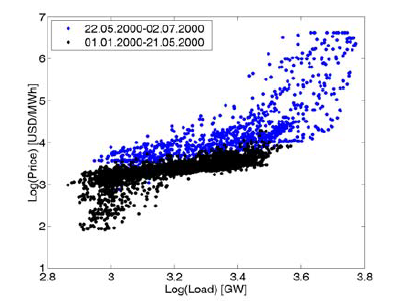
\includegraphics{figures/state_of_the_art/log_loads_vs_log_prices.PNG}
	\caption{The dependence between the
hourly log prices and hourly log system
loads in California for the period January 1
– July 2, 2000. \cite{weron2005forecasting}}
	\label{fig:log_loads_vs_log_prices}
\end{figure}

As can be observed the dependence between loads and energy prices is almost linear except for very low and very high loads, where electricity prices tend to jump to lower and higher values, respectively. 

Results show that for the proposed dataset ARX models (AR with exogenous variables) exhibit lower mean weekly errors (MWE) than AR models which in turn had significantly lower errors than standard ARIMA models. The difference is the separate modeling of individual hours for the ARX and AR models as opposed to an 48 hour aggregate modeling for ARIMA models. 

\subsection{ARIMA models to predict next-day electricity prices}

The authors in \cite{contreras2003arima} propose the application of ARIMA models for day ahead energy price forecasting based on data in the Spanish and Californian power markets. These models are based on time series analysis and results show that accurate electricity price forecasting for the aforementioned power markets is possible. Depending on the market and selected time range average weekly prediction errors 
range from 5\% to 10\%. These results are quite reasonable given that prices from the Californian market in the year 2000 have been selected which has been a very volatile and unstable time period due to the market crash in early 2001 \cite{weron2007modeling}. 

The described model generation process consists of five steps: 

\begin{itemize}
	\item[0)] A class of models is formulated assuming certain hypotheses.
	\item[1)] A model is identified for the observed data.
	\item[2)] The model parameters are estimated.
	\item[3)] If the hypotheses of the model are validated, go to Step 4, otherwise go to Step 1 to refine the model.
	\item[4)] The model is ready for forecasting.
\end{itemize}

This process is taken from the Box Jenkins methodology for forecast model generation \cite{hibon1997arma}.

Interestingly only five hour training periods are needed to model forecasts for the next consecutive hour for Spanish power prices, only two hour training periods are needed for modeling Californian energy prices. 
Through outlier detection the resulting forecasts could have been slightly improved but as stated in \cite{contreras2003arima} this would result in significantly increased computation time. 

%The first step (0) consists of determining a suitable class of models that can be applied to the time series based on observed characteristics, e.g.~high frequency, nonconstant mean and variance, and multiple seasonality. The hypothesis of the model at this step assumes a forecast error term with a normal distribution having a zero mean and constant variance. 
%
%In step 1) a trial model has to be selected for which data has to be made stationary. Through application of a logarithmic transformation a more stable variance can be achieved whereas (seasonal) differencing of data may result in a more stable mean. In order to find appropriate autoregressive and moving average coefficients for the resulting ARIMA model autocorrelation (ACF) and partial autocorrelation (PACF) plots may be consulted to retrieve a first fit of the model. 
%
%Step 2) consists of estimation of parameters which is typically done by applying the maximum likelihood function with respect to the parameters. In order to optimize forecasting performance outlier detection methods may be applied to minimize the impact of single "`spikes"' in the data. 
%
%In step 3) the residuals (forecast errors) of the resulting model are evaluated based on desired characteristics. Residuals should exhibit zero mean, constant variance, should follow a normal distribution and should be uncorrelated. Suitable tests for these properties are portmanteau tests (Ljung box, Box Pierce) and examination of ACF and PACF plots to find dependencies within the data. 
%
%Step 4) is concluding the model selection process. The resulting model of step 2) is used for forecasting based on trained data. 




\subsection{Energy price forecasting approaches in wholesale power markets}

According to \cite{lora2007electricity} electricity price models in general can be classified in two different sets of models, production cost models and statistical models. 

Production cost models retrieve all available information to accurately model system behavior while statistical models are trained on historical data and have little information about the underlying system. An advantage of statistical models is that the amount of information needed to build models is significantly less than that needed for production cost models. 

A taxonomy of electricity price forecasting models is presented in \cite{aggarwal2009electricity} (Figure \ref{fig:classification_of_price_forecasting_models}). 

\begin{figure}[htbp]
	\centering
		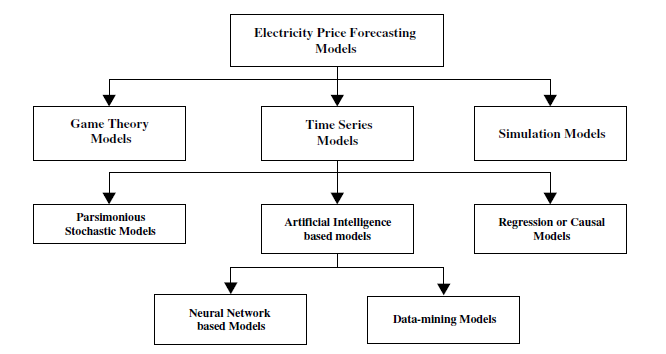
\includegraphics{figures/state_of_the_art/classification_of_price_forecasting_models.PNG}
	\caption{Classification of price forecasting models \cite{aggarwal2009electricity}}
	\label{fig:classification_of_price_forecasting_models}
\end{figure}

In the above taxonomy production cost models are all but parsimonious stochastic models and regression or casual models. Statistical time series models can thus be classified in classical time series models and models based on machine learning approaches \cite{lora2007electricity, duanelectricity}. Classical time series models have the benefit to exhibit a simpler structure than machine learning models, however it is hard to obtain accurate forecasts for non-linear time series such as energy prices. 

Regarding machine learning approaches, artificial neural networks (ANN) have been studied extensively in relation to electricity price forecasting \cite{vahidinasab2008day, singhal2011electricity, pao2007forecasting, amjady2006day, catalao2007short, 
gareta2006forecasting, duanelectricity, szkuta1999electricity}. Neural network models are trained to model non-linear relationships between applicable input variables and historical energy prices. 

Extensive research has been made regarding stochastic time series models as well whereby models may be applied to single \cite{garcia2005garch, weron2008forecastingWh, weron2008forecasting, nogales2002forecasting, cuaresma2004forecasting, tan2010day, conejo2005day} or complex multiple seasonality patterns \cite{de2011forecasting, gould2008forecasting, zivot2003vector}. 
Studies show that univariate time series models may be improved significantly by modeling each hour of the day separately \cite{cuaresma2004forecasting, weron2008forecasting}. However this requires model building separately for each hour which increases the amount of effort needed especially in dynamic forecasting environments. 
It is also stated that including modeling of non-linear phenomena would drastically increase computation time for time series models \cite{cuaresma2004forecasting}. 

%models may be classified in two types: univariate and multivariate time series models. 

Results show that ANN models have the potential to outperform statistical models such as Autoregressive (AR) or Autoregressive Integrated Moving Average (ARIMA) models \cite{pao2007forecasting, catalao2007short}. This may be due to their ability to more accurately model the underlying system behavior while they excel at modeling non-linear relationships in the dataset. 

However, in order to successfully apply forecasting based on neural network models a set of requirements have to be met \cite{catalao2007short}: Availability of sufficient amounts of data, adequate selection of input/output samples, an appropriate number of hidden units and sufficient computational resources. In case these requirements can not be met or it is not possible to appropriately parametrize the model statistical models provide a good alternative for modeling energy prices. 




\section{Cost optimization in geo distributed data centers}

%Different cost optimization approaches have been developed for distributing resources in geographically dispersed data centers. 

\subsection{A Study of Electricity Price Features on Distributed Internet Data Centers}

A comprehensive study about optimization of energy costs under different operational and energy cost prediction regimes is presented in \cite{de2013study}. 

The focus of this work is to leverage price differences across different energy markets in a network of geo distributed data centers to minimize energy costs by migrating resources to currently cheaper locations. It takes into account the impact of several metrics including the level of price variability, time lag between locations, reconfiguration delay and accuracy of energy price predictions. 

To provide a forecasting model based on the given data the Box-Jenkins method is used to build an ARIMA model characterizing the underlying electricity price data:

\[ ARMA(p,q) : P_t = \epsilon_t + \sum_{i=1}^{p}{\phi_i P_{t-i}} + \sum_{j=1}^{q}{\theta_j \epsilon_{t-j}}\] 

where $p$ and $q$ are the number of autoregressive and moving average terms, $\phi_i$ and $\theta_j$ denote the model coefficients and $\epsilon_t$ denotes the error term at time $t$. To accurately model seasonality in the data an $SARIMA(p,d,q)(P,D,Q)[s]$ model has been used which includes the number of terms $p,q$ and $P,Q$ as non-seasonal and seasonal parameters and $d$ and $D$ for non-seasonal and seasonal differencing, respectively. 

Price time series have been generated with different levels of variability $\sigma_{Price}^{2} \in \{50, 126.6, \ab 300, 500\}$. In addition, prediction errors have been used to simulate different forecast accuracy levels, $\sigma_{pred} \in \{2.0, 5.0, 10.0\}$. 

Thus, $P = \{p_1,\ldots,p_T \}$ denotes a price time series and $\hat{P} = \{\hat{p_1},\ldots,\hat{p_T}\}$ a simulation of forecast values such that 
$\hat{P_t} = \mathcal{N}(P_t, \sigma_{pred}), \forall t \in T$. As a measure of accuracy the mean squared error (MSE) has been used: 
$MSE(P,\hat{P}) = \frac{1}{T} \sum_{t \in T}{(P_t - \hat{P_t})^2}$. 

The decision of workload assignment at a particular time $t$ is based on the number of active servers at location $i$ and the corresponding forecast prices $\hat{P_i}(t)$. The total cost at any given moment is defined by $\hat{C_t} = \sum_{i=1}^{N}{m_i \times \hat{P_i}(t) \times Po_i}$ where $Po_i$ denotes the power used by a server running at location $i$ and $m_i$ defines the number of running servers at location $i$. 

Results for different metrics achieved different cost savings \cite{de2013study}. When the number of locations involved in the simulation is increased, cost savings up to 10\% have been reported when going from 1 up to 20 locations. The more locations are considered the greater benefit can be drawn from price differences and time lags between different locations. 

Price variability has been simulated with $\sigma_{price}^{2} \in \{0,5,\ldots,500\}$ and resulting costs have been estimated. It was shown that up to 15\% of savings could be achieved when comparing the maximum and minimum simulated price variabilities. 

Concerning time lags it is stated that the most benefit could be drawn from locations in timezones that are sufficiently distant from each other due to the daily seasonality observed in energy prices. For this scenario up to 15\% cost savings have been achieved for locations that were perfectly "`out of phase"'. 

Finally results show that forecast errors have a major impact on resulting costs. In order to quantitatively measure the impact of forecast deviations $\sigma_{pred}$ has been increased stepwise in the range $0,\ldots,5$ by steps of $0.1$.
The resulting MSE is quadratically rising with the level of $\sigma_{pred}$, thus when errors are at maximum a 10\% revenue loss is expected. 
Therefore accurate forecasts are very important to achieve major cost savings in a multi cloud environment. 




\subsection{Cutting Down the Energy Cost of Geographically Distributed Cloud Data Centers}

This paper aims to minimize energy costs in geographically distributed data centers by taking into account spatio-temporal variation in electricity prices and the outside weather temperature \cite{guler2013cutting}. The scenario is modeled as a linear programming problem which is solved by presenting various heuristic solutions to the problem. 

While providing algorithms for minizing energy costs resulting SLA penalties as well as cooling related costs are taken into account. 
For each data center a performance coefficient (CoP) is calculated which is based on outside weather temperature where the coefficient increases linearly with rising temperature. A data center may have different types of servers exhibiting different performance metrics and capacities. 

Energy costs are calculated as the sum of server power consumption over a specific time range multiplied by the applicable energy prices during that time. 
The total costs for data center $i$ are defined as $E_{i}^{total} = E_{i}^{IT} \times CoP(T_i)$ where $T_i$ denotes the temperature at location $i$. 

The actual time a job $j$ needs when running on a type $k$ server $s$ is defined as 
\[  T_{j,s} = \frac{c_j \times f_j \times l_j}{c_k \times f_k}  \] 
where $c$ and $f$ denote the number of cores and frequency available / needed by a server / job and $l$ denotes the expected runtime of job $j$. 
A penalty occurs if the total runtime of a job exceeds the expected runtime when running on server $s$. 

The goal is to minimize the sum of total energy and penalty costs over all data centers 
\[ \min \sum_{i=1}^{N}{E_{i}^{total} + Pen_i} \]
where $Pen_i$ denotes the total penalty cost for data center $i$. 

Based on the proposed linear optimization problem two types of scheduling algorithms are introduced, immediate and delayed. Immediate scheduling algorithms are defined as CheapestDC and CheapestS where the former places resources randomly on hosts located at the currently cheapest data center while the latter includes outside weather temperature as well in the calculation. Delayed scheduling algorithms additionally consider historical energy prices to decide whether jobs should be delayed to a future time stamp. 

Simulation runs over six data centers at different locations handling three types of workloads were conducted to evaluate different scheduling algorithms.
Results show that delayed scheduling techniques on light workloads achieve over 5\% on overall cost savings compared to the baseline random scheduler. Also, spatial electricity price variations have the most impact on cost savings followed by temporal electricity price changes and reduced cooling costs due to outside weather temperature. 


\subsection{Studies for cost optimizations in multi-electricity-market environments}

Different studies have been developed for optimizing energy costs in multi market environments. 

In \cite{buchbinder2011online} the basic tradeoff between energy and bandwidth costs is discussed for migrating virtual machines between geographically distributed data centers. 
Three different algorithms have been evaluated on a set of 30 US locations covering three years of next day electricity data. Out of the two greedy algorithms and the online migration algorithm the latter provided the best results with only 4 to 6 \% off the optimal offline solution. 

The authors in \cite{rao2010minimizing} aim to minimize energy costs while guaranteeing quality of service by referring to a constrained mixed integer programming model. The approximated linear programming model is converted to a minimum cost flow problem which can be solved fast and efficiently. With five frontend web portal servers targeting three internet data centers cost reductions up to 30\% are achieved within the simulation. 

An extensive study on electricity price features and its implications for existing cloud systems is given in \cite{qureshi2009cutting}. While taking into account server energy elasticity and bandwidth constraints a maximum cost savings of 45\% could be achieved when running a simulation over 39 months including 29 locations. However, in order to achieve these results bandwidth constraints are relaxed and large distances to clients have to be permitted. 

A different approach is examined by \cite{simarro2011dynamic} where dynamic pricing schemes of different cloud providers are taken advantage of to reduce investment of users. The assumption is that prices for each cloud provider change according to demand and thus virtual cluster placements can be optimized across different cloud providers. As infrastructure is dynamically distributed without notice of the user it provides an efficient and convenient way of reducing costs for cloud users. 

Cost based multi cloud schedulers have been investigated in \cite{le2009cost} and \cite{tordsson2012cloud}. 
A cloud scheduler for simplified management of virtual machines has been developed in \cite{armstrong2010cloud}, a green cloud scheduler in \cite{lucanin2013take}. 
Also, schedulers based on genetic algorithms were proposed by \cite{dutta2011genetic} for cost based multi QoS optimizations and \cite{ge2010ga} for improving delay scheduling policy. 



\section{Optimize resource scheduling in data centers}

\subsection{A task scheduling algorithm based on load balancing in cloud computing}

In \cite{fang2010task} a two level scheduling model has been implemented (Figure \ref{fig:two_level_resource_scheduling}). 

\begin{figure}[htbp]
	\centering
		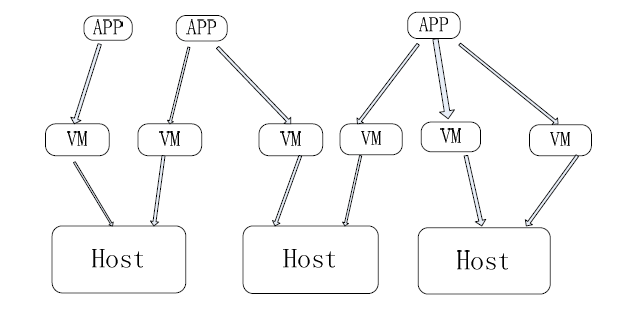
\includegraphics[width=0.7\textwidth]{figures/state_of_the_art/two_level_resource_scheduling.PNG}
	\caption{Two level scheduling model \cite{fang2010task}}
	\label{fig:two_level_resource_scheduling}
\end{figure}

A two stage process is described where the first scheduler creates the task description of a virtual machine s.t.~the task will have a perfect fit on a virtual machine whereas the second scheduler is responsible to find appropriate resources (hosts) for the provisioned virtual machine. Thus an optimized resource scheduling is presented with focus on load balancing among different clouds. 

Tasks have a defined structure where task $t_i$ out of the set of all Tasks $T$ is defined as 

\[t_i = \{tId, tRr, tSta, tData, tVmch, tVm\}\]

\begin{itemize}
	\item $tId$ is the task identification
	\item $tRr$ denotes the required resources
	\item $tSta$ describes the state of the task where $tSta = \{tFree,tAllo,tSche,tWait,tExec,tComp\}$
	\item $tData$ defines the relative data of the task (computational load, input and output data)
	\item $tVmch$ denotes the virtual machine specification where $tVmch = \{tId,tRr,tData\}$
	\item $tVm$ defines the assigned virtual machine of the task where $tVm = \{tId,thId\}$
\end{itemize}

Hosts on the other hand are defined as $h_j = \{hId, hTcap, hFcap, hData\}$, where

\begin{itemize}
	\item $hId$ denotes the host identification
	\item $hTcap$ is the total host capacity (set of resource capacities)
	\item $hFcap$ is the freely available host capacity
	\item $hData$ denotes the relative data of the host (including input and output bandwidth)
\end{itemize}

%Concerning the scheduling algorithm, the predicted task resource usage is defined as $VL_i$. 

The scheduling algorithm is based on the following equations: 

\[ HL_i = \frac{\sum_{j=1}^{n}{VL_j}}{n} \]

\[ avgl = \frac{\sum_{i=1}^{m}{HL_i}}{m} \]

\[ B = \frac{\sqrt{\sum_{i=1}^{m}{(HL_i - avgl)^2}}}{m} \]

where $VL_j$ is the predicted resource load for VM $j$, $HL_i$ is the average load for host $i$, $avgl$ denotes the average
load across all running hosts and $B$ denotes a metric for load balancing. 

The scheduler iterates over the set of hosts in each timestamp and determines the value of the load balancing metric $B$. In case the value of 
$B$ exceeds a predefined threshold $B_0$ or the predicted resource requirements for a virtual machine exceed the currently allocated resources 
the VM is migrated to a host occupying the least resources for optimal load balancing. 

Results show that considering dynamic resource requirements load is distributed across all machines leading to stable level of cloud utilization. 



\subsection{Efficient resource management for cloud computing environments}

In \cite{younge2010efficient} power aware and live migration scheduling techniques are proposed as a green cloud approach to increase overall system efficiency with minimal performance overhead. 

A new greedy based algorithm is presented to minimize power consumption. It is based on the findings that power consumption of a server does not increase linearly with the number of cores utilized. Instead, most power is drawn by one utilized core whereas power increases only slightly when comparing a server utilizing 7 to 8 cores. Thus a new VM scheduling algorithm is proposed that minimizes resulting power consumption within a data center. 

Hosts are assigned to a pool of resources where a pool can be initialized by a priority based evaluations system to either maximize performance or further minimize power consumption \cite{younge2010efficient}. Each VM request is checked against its resource requirements and available capacities in the pool and assigned to a host to maximize utilization and therefore minimize overall power consumption. 

In addition, live migration of virtual machines is applied to further optimize power consumption by shifting load away from under utilized hosts (Figure \ref{fig:server_power_consumption}). When load increases, Wake on Lan (WOL) technology is used to power servers back up again. Furthermore, a focus has been to reduce VM image size and boot time to optimize virtual machines for a server environment. 

%\begin{figure}[htbp]
	%\centering
		%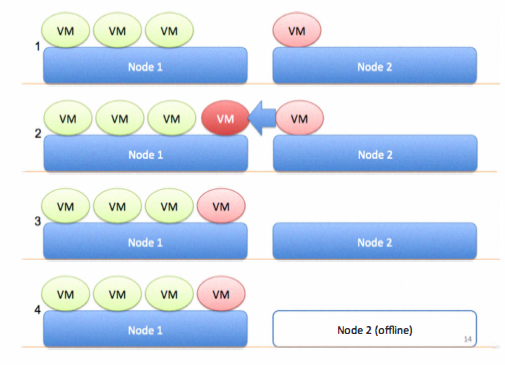
\includegraphics{figures/state_of_the_art/vm_migration_for_host_consolidation.PNG}
	%\caption{Virtual machine management dynamic shutdown technique \cite{younge2010efficient}}
	%\label{fig:vm_migration_for_host_consolidation}
%\end{figure}

\begin{figure}[htbp]
	\centering
		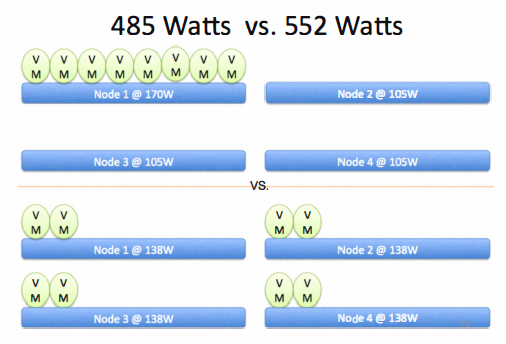
\includegraphics{figures/state_of_the_art/server_power_consumption.PNG}
	\caption{Illustration of scheduling power savings \cite{younge2010efficient}}
	\label{fig:server_power_consumption}
\end{figure}

Power aware resource scheduling has been simulated on an OpenNebula \cite{fontan2008opennebula} pool of 4 servers, equipped with 8 cores each. Power elasticity (power range from idle to peak power of a server) for this type of server is 61\% where a total reduction in power consumption of 12\% could be achieved. As the results are scalable also to large clusters significant power and cost savings are possible using the proposed approach. 


%
%Active research topics in this field include electricity cost reduction in data centers \cite{guler2013cutting, le2011reducing}. A comparison of different approaches considering spatial and temporal energy price changes and the contribution of the outside temperature to the resulting cooling effort and expense is outlined in \cite{guler2013cutting}. In \cite{le2011reducing} a set of homogenous data centers is simulated where the focus lies on the effects of changing workloads and migrations on the cooling infrastructure and on intelligent scheduling to reduce energy consumption and energy costs, respectively. 
%
%The authors in \cite{lucanin2013take} propose a green cloud approach using real time electricity prices where the duration and time of price peaks are estimated and VMs are paused during these times to reduce energy costs and save energy. Customers may choose between ``green'' and normal instances, taking into account some loss of availability for a reduced price. 
%
%
%
%In \cite{rao2010minimizing} a cloud consisting of several Internet Data Centers (IDC) is examined with regard to cost optimization which is done by intelligently assigning workload to data centers based on current energy prices. Two of these data centers in the scenario are connected to deregulated wholesale energy markets whereas the other one is connected to a regulated utility region charged by a fixed pricing scheme. Since price change differences in deregulated energy markets can be considerable energy cost reductions may be achieved by assigning workload based on changing energy prices.  %For the purpose of the simulation five front-end Web portal servers process a total workload of about $10^5$ requests per second. 
%
%In this paper the approaches of optimal and average workload assignments are visually and formally compared to gain insights into the total electricity cost reduction. The optimal workload assignment is calculated with respect to workload and delay constraints that are considered in a minimum cost flow problem based on a linear programming model. Thus the goal is to minimize costs without compromising quality of service constraints. 
%%The proposed cost reductions amount up to 30 percent for a single hour test within the given time range. 
%%The results measured at two timestamps at a specific day seem promising, since total cost reductions could be achieved by 30\% and 17\% respectively. 
%
%The differences compared to this work is that in \cite{rao2010minimizing} they do not consider longer running jobs as used in scientific calculations or large optimization problems that may take several hours to complete. Thus the impact of migrations is not examined in this scenario. In addition the possibility of energy price forecasting is not considered which may result in even greater energy cost reductions. 
%
%Another study on cost reductions in Internet Data Centers has been done where different aspects of cost reductions including cost prediction schemes have been considered \cite{de2013study}. Since up to 15\% of total capital investment is spend on energy related costs 
%%(paper references \cite{greenberg2008cost} - old, from 2009!!) 
%a special effort is invested to reduce the amount of energy costs through cost aware operations. %(TODO: Move to introduction?)
%
%In this paper cost optimization is seen as an assignment problem where an overall cost function is minimized through intelligent workload allocation. During the investigation different variables and their impact on resulting energy costs are considered which are price volatility, price predictions including variable prediction errors, time lag between locations and reconfiguration delays. 
%
%Similar to this work the simulation is run with the same set of fixed parameters to evaluate the impact of the various scenarios. It is observed that prediction errors greatly impact workload allocation where cost penalties due to non-optimal assignments increase quadratically with an increase of forecast errors \cite{de2013study}. Also with increasing number of locations the minimum cost of optimal assignments can be greatly reduced. Greater price volatility is beneficial as well since then price aware assignments will have greater impacts. 
%
%A comprehensive study on cost reductions and energy market characteristics in an environment where data centers are placed within the reach of different energy markets is presented at \cite{qureshi2009cutting}. Based on geotemporal variations of energy prices the maximum cost reductions under different scenarios are evaluated. Energy expenses are estimated for various large scale companies like Google and Yahoo to state the actual savings and the amount of reductions in energy costs that would be possible. 
%They also discuss the impact of considering bandwith constraints and maximum client server distances on cost reductions. 
%
%Interestingly enough long term seasonalities in the energy price data has been discovered that spanned multiple energy markets. This is an important fact when training forecasting models since predictions can become a lot more accurate. An important fact that was revealed about energy markets was that data from different energy markets was much less correlated than data from the same area. Thus to take full advantage of energy price differences data centers located at different energy markets should be combined \cite{qureshi2009cutting}. 
%
%With different state of the art energy models and simulation constraints a summary of possible cost reduction schemes was presented. However no migration or forecasting of energy price data has been done which could further improve scenarios with longer running jobs. In addition these cost reductions are only valid under specific assumptions that large cloud providers would need to implement such as connection to wholesale energy markets and reasonable server energy elasticity. 
%
%
%
%
%\subsection{Server power management}
%
%A well known problem in power management is how to accurately and efficiently model a server's power consumption over time. At \cite{horvath2008multi} Horvath et al.~exploit dynamic voltage scaling (DVS) and multiple sleep states to reduce power consumption of a server cluster of about 23\% without significantly impacting performance. They propose that CPU utilization and frequency are the variables that have the most significant impact on the power consumption of a machine. This assumption is also used in other studies, e.g.~\cite{rao2010minimizing, hammadi2014survey, kliazovich2012greencloud}. 


\section{Virtual machine migration}
%\subsection{Virtual machine migration in cloud environments}


Live Virtual machine migration is defined as follows:
\begin{quote}
A source virtual machine (VM) hosted on a source server is
migrated to a destination VM on a destination server without
first powering down the source VM \cite{nelson2009virtual}.
\end{quote}

Thus efficient methods for transferring VM memory pages from the source to the destination host are needed which will be evaluated in the following sections. 
%One method is defined by resuming the destination VM before all memory pages from the source VM are transferred. This can be done by paging in any remaining VM memory pages from the source to the destination on demand. A second approach executes a pre-copy phase where memory is transferred in several rounds from the source to the destination host before launching the destination VM. Dirtied memory pages are re-transferred which have been dirtied during previous transfers of memory to ensure a consistent VM memory image at the destination. 
%
%The non-memory state of the VM is preferably available in a shared storage arrangement accessible by both the source and destination VMs such that it is only required to re-map the source VM's virtual disk to the destination VM. In case no shared storage is available, the source VM's non-memory state has to be transferred to the destination VM before or after the migration depending on the implementation. 


\subsection{Live migration of virtual machines}

In \cite{clark2005live} an efficient approach for live migration of virtual machines is presented. This paper targets the migration of entire OS within a virtual machine without noticeable service interruption. 

The applied method for migration should minimize both downtime and total migration time for the virtual machine. The first metric denotes the actual downtime of the VM where it is completely suspended and unaccessible to users. The second metric is defined by the total time between the start of the migration process until its end \cite{clark2005live}. 

Three methods have been identified that have been used previously. The \textit{pure stop-and-copy} approach halts the source VM, copies all memory pages to the destination host and resumes execution at the destination. Both downtime and total migration time are proportional to the amount of memory to be transferred which can lead to unacceptable downtimes. 

The \textit{pure demand migration} method is defined where essential data for running the VM is transferred to the destination host after which the destination VM is booted. Any missing memory pages create page faults and trigger a synchronous transfer from the source host on first use. This leads to poor performance until a sufficient amount of memory pages have been transferred. 

The \textit{pre-copy} approach combines an iterative push-phase with a very short stop-and-copy phase to minimize downtime. Any pages dirtied during a transfer of memory are re-sent in the next iteration until a sufficient amount of memory pages have been transferred to the destination host. In a final stop-and-copy phase the VM is suspended on the source host, remaining memory pages are copied to the destination and the VM is resumed at the destination. 

An important efficiency measure for VM migrations has been identified as the writable working set (WWS) \cite{clark2005live}. It is defined as a set of memory pages that are updated very frequently such that it is not worth keeping them consistent at the source and destination hosts. These set of pages should be copied only in the final stop-and-copy phase. An accurate measure of the WWS for the SPEC CINT2000 benchmark is depicted in Figure \ref{fig:tracking_writable_working_set}. 

In this graph the number of 4KB pages of memory dirtied within a corresponding 8 second interval are shown for each of the programs run in the benchmark. 
It is clearly visible that the number of pages contained within a WWS depends greatly on the behavior of the selected program. Workloads exhibiting a high amount of frequently updated pages such as \textit{gap} will provide only a small number of pages sensible for inclusion in a pre-copying phase. 
Thus the downtime and cost resulting from a VM migration depends to a great extent on the type of workload being migrated and the exact moment of the start of the migration. 

%Thus the source virtual machine does not hold any dependencies related to the destination VM after migration has finished. The in-memory state of the VM is transferred efficiently such that a seamless live migration becomes possible. 


\begin{figure}
	\centering
		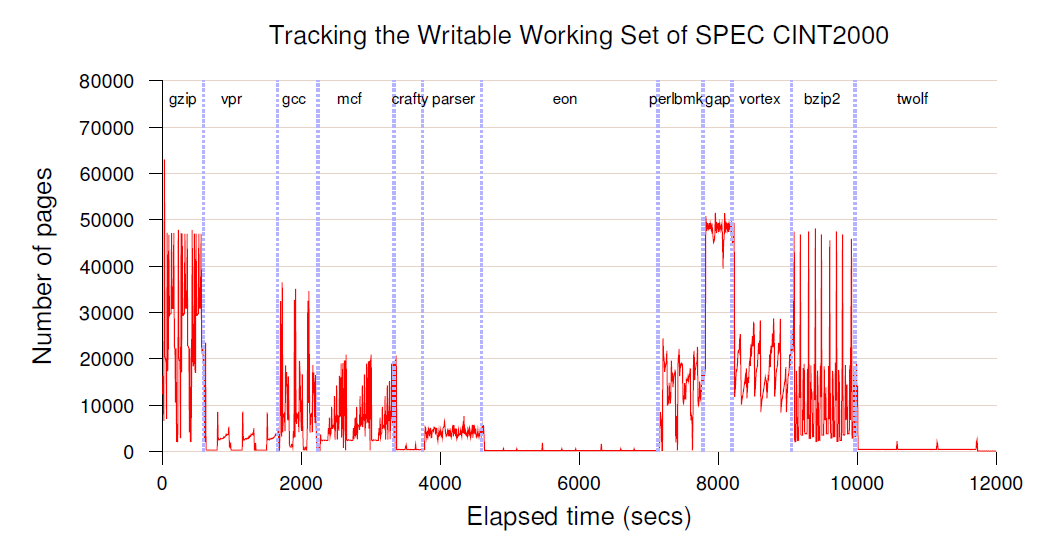
\includegraphics[width=1.0\textwidth]{figures/state_of_the_art/tracking_writable_working_set.PNG}
	\caption{WWS curve for a complete run of SPEC CINT2000 (512MB VM) \cite{clark2005live}}
	\label{fig:tracking_writable_working_set}
\end{figure}



Results for different kind of workloads indicate that even in the worst case the pre-copy approach significantly reduces downtime compared to the stop-and-copy method. As bandwidth has a direct impact on migration downtime performance can be further increased by raising the bandwidth assigned to the VM migration. 

Migration downtimes have been evaluated for different sized VMs running various kinds of workloads. Resulting downtimes range from only 60 ms for small sized VMs (64 MB) and low dirty page rate to 3.5 seconds for large VMs (512 MB) with frequently updated dirty page rates. It is stated that realistic workloads can be migrated with a downtime as low as 210 ms in a virtualized cluster environment. 


\subsection{Performance and energy modeling for live Migration of Virtual Machines}

A thorough evaluation of migration performance and resulting migration costs is given by \cite{liu2013performance}. 

The authors provide methods to quantitatively predict migration performance and resulting energy cost. A refined pre-copy approach is used to efficiently transfer memory pages in iterative rounds where in each round the memory pages dirtied in the previous round are re-sent (Figure \ref{fig:VM_migration_precopy}). 
The pre-copying phase is terminated when any of the following conditions are satisfied:

\begin{enumerate}
	\item [1)] memory dirtying rate exceeds memory transmission rate
	\item [2)] the remaining dirty memory falls below a predefined threshold
	\item [3)] the number of pre-copying iterations exceeds a defined maximum
	\item [4)] total network traffic exceeds a multiple of the VM memory size
\end{enumerate}

\begin{figure}[htbp]
	\centering
		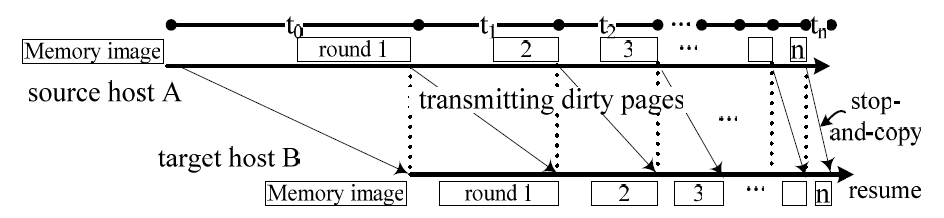
\includegraphics[width=0.7\textwidth]{figures/state_of_the_art/VM_migration_precopy.PNG}
	\caption{Live migration algorithm performs pre-copying in iterative rounds \cite{liu2013performance}}
	\label{fig:VM_migration_precopy}
\end{figure}

Findings in this work include that with incremental data transmission rate (bandwidth) the power consumption progressively increases while the migration latency decreases. Also, power consumption during migrations increase for both source and destination hosts from which the resulting migration energy can be derived. In addition the migration load and time needed for each pre-copy iteration as well as the total migration load and latency are calculated. 

Besides the defined base model a refined migration model is specified which takes into account the size of a workload's writable working set, that is the number of pages dirtied most frequently. The latter model has been empirically evaluated by measuring the WWS on a Xen virtual machine and deriving the maximum sensible pre-copy iteration while continuously checking termination conditions. 

\begin{figure}[htbp]
	\centering
		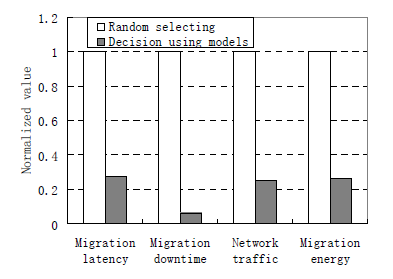
\includegraphics{figures/state_of_the_art/vm_migration_normalized_cost.PNG}
	\caption{Migration cost savings by using proposed models \cite{liu2013performance}}
	\label{fig:vm_migration_normalized_cost}
\end{figure}

Workloads with different sizes for writable working sets have been evaluated in simulations including two hosts running 8 virtual machines. 
The resulting migration downtime, migration latency, network traffic and energy consumption could be reduced by 72.9\%, 93.5\%, 74.5\% and 73.6\% compared to a random selection technique, respectively (Figure \ref{fig:vm_migration_normalized_cost}). 





%Migration costs and downtime may vary significantly depending on the type of workload and VM configuration parameters. The authors leverage cost prediction schemes to yield expected costs for specific VM migrations. 









%See "`Live Virtual Machine Migration via Asynchronous Replication and State Synchronization"'
%
%\begin{figure}[htbp]
	%\centering
		%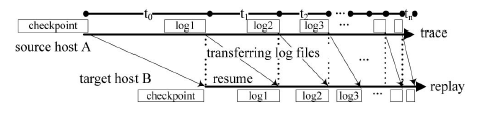
\includegraphics{figures/state_of_the_art/virtual_machine_precopy.PNG}
	%\caption{Migration process ideal case}
	%\label{fig:virtual_machine_precopy}
%\end{figure}

%
%\begin{figure}[htbp]
	%\centering
		%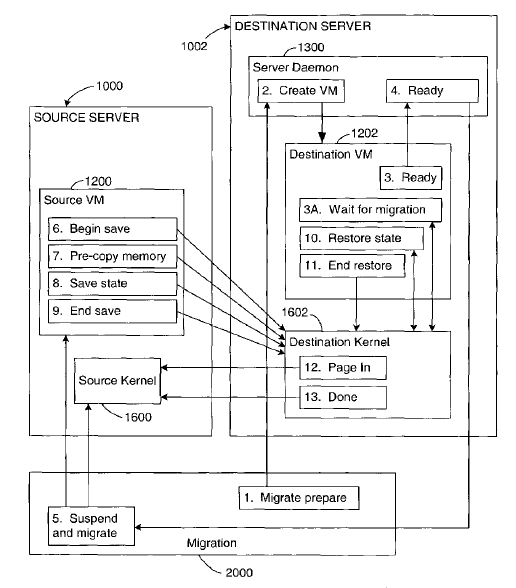
\includegraphics{figures/state_of_the_art/virtual_machine_migration.PNG}
	%\caption{Virtual machine migration}
	%\label{fig:virtual_machine_migration}
%\end{figure}


%There are different proposed approaches related to virtual machine migration in distributed cloud environments \cite{celesti2010improving, malet2010resource}. In \cite{celesti2010improving} the so-called Composed Image Cloning (CIC) methodology designed for migration of VMs across federated clouds is introduced. This work aims to reduce the needed bandwidth and migration time by setting up a new virtual machine in the destination cloud and transferring only user data instead of relocating the whole VM disc image. 
%
%In another work \cite{malet2010resource} the placement of applications is dynamically adjusted across distributed data centers according to the location of the currently highest request rate. 




%%%%%%%%%%%%%%%%%%%%%%%%%%%%%%%%%%%%%%%%%
\chapter{Data Analysis}
\label{ch:data_analysis}
%%%%%%%%%%%%%%%%%%%%%%%%%%%%%%%%%%%%%%%%%





\section{Day ahead and real time energy prices}




\section{Characteristics of energy markets}

Ideas: 

\begin{itemize}
	\item Show electricity price variation for market over a 3 year period (Weron, pg 33)
	\item Show autocorrelation function over extended (same) time period
	\item Show periodogram over extended time period
\end{itemize}




See folders "`Electricity pricing"' and "`power markets"'


\begin{figure}[htbp]
	\centering
		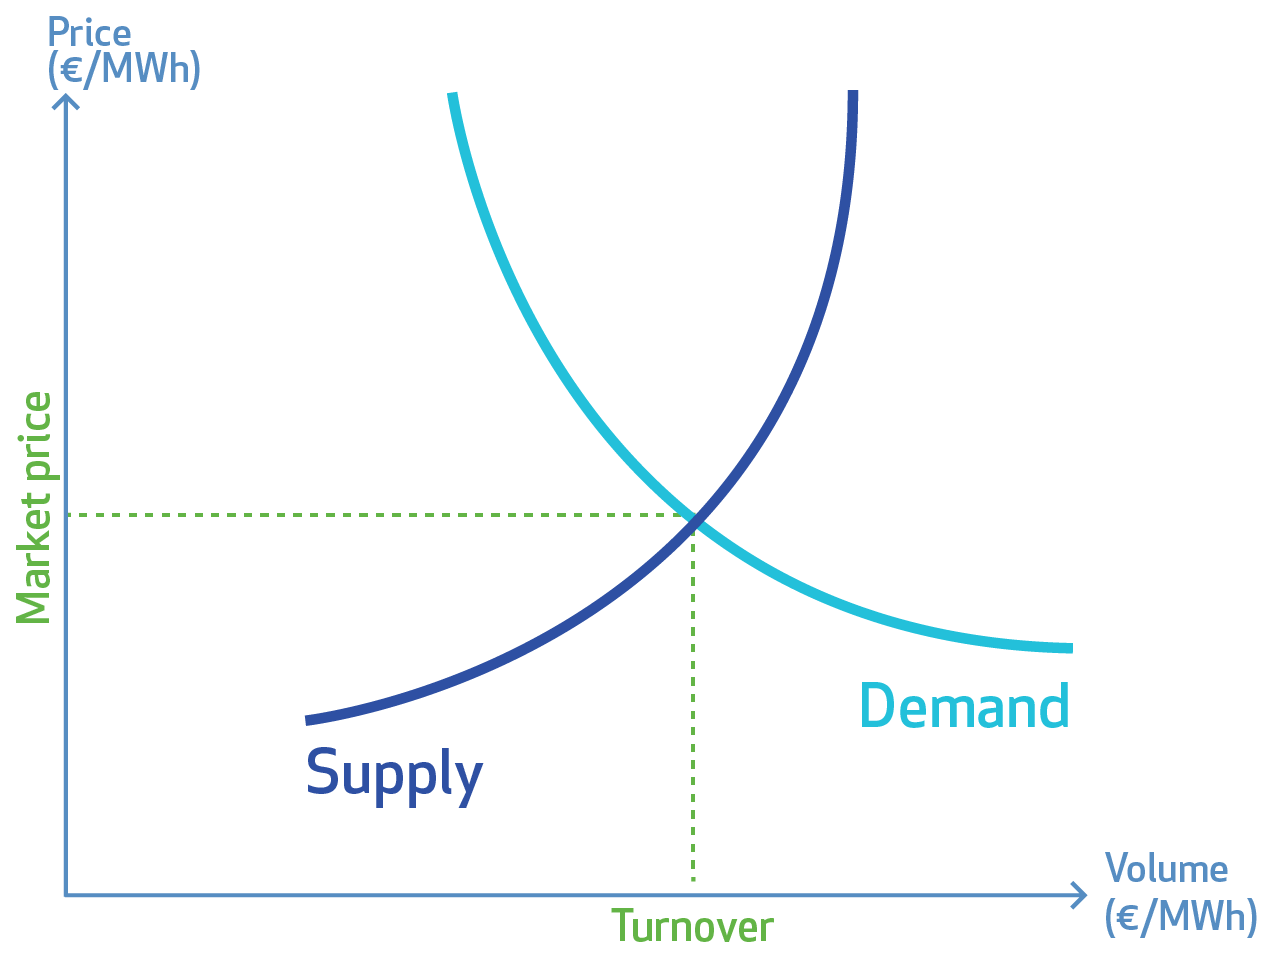
\includegraphics[width=0.5\textwidth]{figures/data_analysis/DA_supply_demand.png}
	\caption{Intersection between supply and demand \cite{nord2014supply}}
	\label{fig:DA_supply_demand}
\end{figure}



In this section different studies of power market characteristics are presented to distinguish features that may be used in building forecasting models. 

\subsection{Stable Modeling of different European Power Markets}

In this paper different European power markets have been investigated to reveal major differences in energy price behaviour \cite{mugele2005stable}. The EEX, Nord Pool Spot and Polish power markets have been evaluated whereby the markets are responsible for the Mid-Europe, Northern Europe and Polish regions respectively. 

As in general electricity prices depend on energy demand \cite{weron2005forecasting} which changes due to climate conditions (temperature and number of daylight hours) electricity prices exhibit a seasonal component as well (Figure \ref{fig:seasonal_behaviour_of_eex_prices}). 

\begin{figure}[htbp]
	\centering
		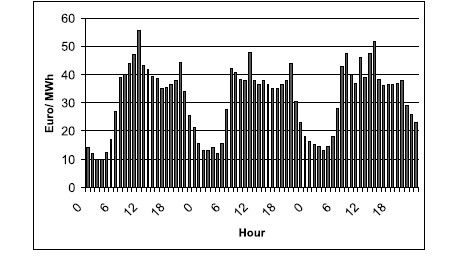
\includegraphics{figures/state_of_the_art/seasonal_behaviour_of_eex_prices.PNG}
	\caption{EEX - hourly spot prices \cite{mugele2005stable}}
	\label{fig:seasonal_behaviour_of_eex_prices}
\end{figure}

The main differences between electricity power markets and other financial markets are price volatility, mean reversion and price jumps or "`spikes"'. Volatility is high as generated electricity cannot be stored but has to be delivered at once which might lead to high prices on transmission congestion or surges in demand. It's impact can be reduced by applying logarithmic transformations of input data \cite{weron2005forecasting}. 

Energy prices experience strong mean reversion which denotes the characteristic that prices return to their mean levels after an increase in prices. In addition price spikes may appear where prices can increase tenfold from one hour to the next. To mitigate these spikes they may be averaged out in a data preprocessing step. 

Even though price seasonality and trend seem to be stable over a short time range (Figure \ref{fig:seasonal_behaviour_of_eex_prices}) they can show significant fluctuations over a longer time range. In \cite{mugele2005stable} data related to each examined energy market was fitted to a stable Paretian distribution as well as a normal distribution. The result showed that mature markets as EEX or Nord Pool Spot exhibit high volatility, heavy tails, high kurtosis and asymmetrics in the energy price data which was best modeled by the Paretian distribution. In contrast the Gielda Energii SA market in Poland shows a much more stable energy price behavior which can be modeled by a Gaussian distribution. 

The variation in energy price levels for the two power markets EEX and Nord Pool Spot are shown in Figures \ref{fig:EEX_levels} and \ref{fig:NordPool_levels}.

\begin{figure}[!htbp]
  \centering
  \begin{minipage}[b]{0.4\textwidth}
    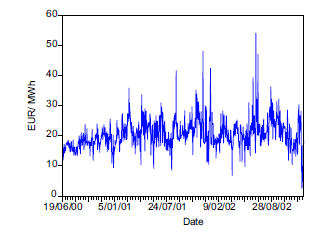
\includegraphics[width=\textwidth]{figures/state_of_the_art/EEX_levels.PNG}
    \caption{EEX levels \cite{mugele2005stable}}
		\label{fig:EEX_levels}
  \end{minipage}
  \hfill
  \begin{minipage}[b]{0.4\textwidth}
    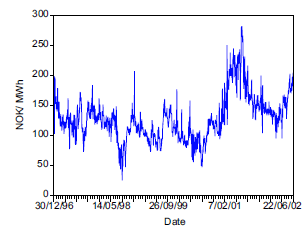
\includegraphics[width=\textwidth]{figures/state_of_the_art/NordPool_levels.PNG}
    \caption{Nord Pool levels \cite{mugele2005stable}}
		\label{fig:NordPool_levels}
  \end{minipage}
\end{figure}

This shows that it is important to investigate energy price characteristics from power markets to accurately model market prices. 



%
%\subsection{Electricity markets and pricing}
%
%In wholesale energy markets different pricing and bidding models can be used. Currently the two most common price evaluation strategies are day-ahead and real-time pricing strategies. 
%
%\subsubsection{Bidding strategies}
%
%In \cite{tierney2008uniform} two different bidding strategies are discussed, uniform pricing and pay-as-bid auctions. In the uniform pricing model the market clearing price is determined by collecting the marginal prices from all suppliers and taking the maximum price from this collection. Conversely, in pay-as-bid auctions a supplier gets paid based on its actual bid. 
%The second approach may seem beneficial from the customer's point of view since suppliers may set individual prices which enables competition within the market. 
%However studies show that in this pricing scheme suppliers set their prices at the maximum possible level to be comparable to other suppliers and keep their customers. On the other hand the uniform pricing model provides a uniform clearing price which is valid for all participants in the market and customers may trust that suppliers set prices to just satisfy their needs. 


\section{Energy price case study}





%%%%%%%%%%%%%%%%%%%%%%%%%%%%%%%%%%%%%%%%%
\chapter{Forecasting}
\label{ch:forecasting}
%%%%%%%%%%%%%%%%%%%%%%%%%%%%%%%%%%%%%%%%%


\section{Introduction}

As outlined in \ref{sec:electricity_price_forecasting} different types of models have been investigated for forecasting spot electricity prices. In this work forecasting models should be used that exhibit the following characteristics: 

\begin{itemize}
	\item computationally lightweight
	\item capable of modeling seasonality
	\item capable of recognizing trends in the dataset
	\item good out-of-sample accuracy based on day ahead and real time electricity prices
	\item capable of being part of an automated model generation process
	\item accurate modeling of different energy price characteristics
\end{itemize}

Statistical models have been proven to provide good results and at the same time keeping the computational effort low \cite{aggarwal2009electricity,bunn2003forecasting}. In contrast structural or non-parametric models require additional input data and perform more complex operations such that they might not be the optimal choice for dynamic forecast environments. Therefore models in this work have been chosen from the well known set of parsimonious stochastic models. 

Different stochastic models are able to generate forecasts while considering existing seasonality in the data \cite{gould2008forecasting,de2011forecasting}. Examples of models exhibiting these characteristics are SARIMA, HoltWinters and TBATS, all of which are investigated in this work to evaluate their capability of forecasting on different settings and datasets. The best model is then chosen to provide forecasts for all simulations described later in this work. 

In general time series may be decomposed into seasonal, trend and cycle components which can be made use of by forecast models \cite{de2011forecasting}. Some models such as ARIMA and TBATS can handle existing trends in the dataset by applying transformations in a preprocessing step or by decomposing and separately modeling time series components. More simplistic models such as Simple Exponential Smoothing (SES) or pure Autoregressive (AR) models require the dataset to be stationary, i.e.~to exhibit a constant mean and variance \cite{weron2007modeling,hyndman2012forecasting}. In this case the dataset would have to be transformed before applying those models. 

Models should provide good out-of-sample accuracy which means that they need to be trained and tested on different datasets \cite{hyndman2012forecasting}. For example, considering training data from a training period of four weeks of energy price data and test data from a subsequent test period of one week a model is trained based on that training data but tested on the provided test data. Thus real life forecasting scenarios can be established and models are evaluated based on the accuracy on test datasets. A large scale evaluation of forecasting models based on different trainings and test datasets is presented later in this section. 

Building an automated model generation process is important for automatic model evaluation and model selection for simulations running over a longer period of time. As extensive simulations including forecasts represent a core contribution of this work an automated model generation process has been defined including preprocessing steps and model evaluation to find the best suited model for a given dataset. 

Inclusion of energy price characteristics such as mean reversion and price spikes into forecast model generation has been studied extensively considering different types of forecast models \cite{weron2008forecasting,bunn2003forecasting,aggarwal2009electricity}. Mean reversion denotes the characteristic that a time series returns to its mean after significant deviation. This characteristic is modeled by a AR(1) process and can be incorporated e.g.~into an ARIMA model. For handling price spikes three approaches have been defined in literature \cite{weron2008forecasting}: 1) Using models that allow spikes in input datasets 2) Remove price spikes completely from the data 3) Recognize and dampen observed spikes to mitigate their impact on out-of-sample forecasts. For simplicity reasons price spikes have not been modeled explicitly in this work meaning they are not dampened or removed from the datasets. 



\section{Methodology}

In this section the various methodologies used in the forecasting framework are discussed. 

%It presents seasonality estimation, time series decomposition, selected forecast models, model selection algorithm, the forecast simulation framework and a forecast model evaluation implemented on a large scale. 


\subsection{Seasonality estimation and periodogram}

Estimating seasonality is an important pre-processing step when building forecasting models. As most models are not able to automatically detect seasonality in the given data it is vital to determine possible seasonality cycles beforehand. 

One way of detecting seasonality in the data is by doing a spectral analysis for exploration of cyclical patterns. 
During the process the data is decomposed into underlying sinusoidal (sine and cosine) functions with particular wavelengths \cite{weron2007modeling}. 
The wavelength is commonly described as frequency which is the number of cycles per unit time. 

The frequency $\omega$ and the period $T$ have a reciprocal relationship $\omega = \frac{1}{T}$. Thus the period $T$ denotes the number of unit time stamps required to complete one period which in case of daily seasonality in a time series of hourly observations can be 24 time stamps, i.e.~24 hours. 

In order to visualize common frequencies a \textit{periodogram} may be generated which can be regarded as a tool for retrieving the most common frequencies from the dataset. As existing seasonality patterns in the data are likely to be detected by the periodogram as high valued frequencies it can be used to extract these frequencies and calculate the reciprocal as the seasonal period $T$. 

The formula of a periodogram for a vector of observations $\{x_1,\ldots,x_n\}$ is defined as \cite{weron2007modeling}:

		\[ I_n (w_k) = \frac{1}{n} \left| \sum_{t=1}^{n}{x_t  e^{-i(t-1) \omega_k} } \right|^2 \]
		
		where $\omega_k = 2 \pi (k/n)$ denote the Fourier frequencies in radians per unit time, $k = 1,\ldots,[n/2]$ and $[x]$ describes the largest integer value less than or equal to $x$. 

Figure \ref{fig:periodogram_July_2014} shows a periodogram of two weeks of hourly day ahead prices from the Nord Pool Spot power market. 
On the x-axis frequencies from 0 to 0.5 are displayed, on the y-axis each frequency's corresponding value is depicted, proportional to the number of occurrences of this frequency. In case of a random signal the frequencies should be uniformly distributed across the frequency scale. In this case clearly two frequency values stand out where the values are of magnitudes $\omega_1 = 0.0416$ and $\omega_2 = 0.0833$. This results in periods $T_1 = 24$ and $T_2 = 12$, which means that the underlying series exhibits a strong daily seasonality of 24 hourly prices with a so called \textit{harmonic} of 12 periods which denotes a multiple of the 24 hour period. 


\begin{figure}[htbp]
	\centering
		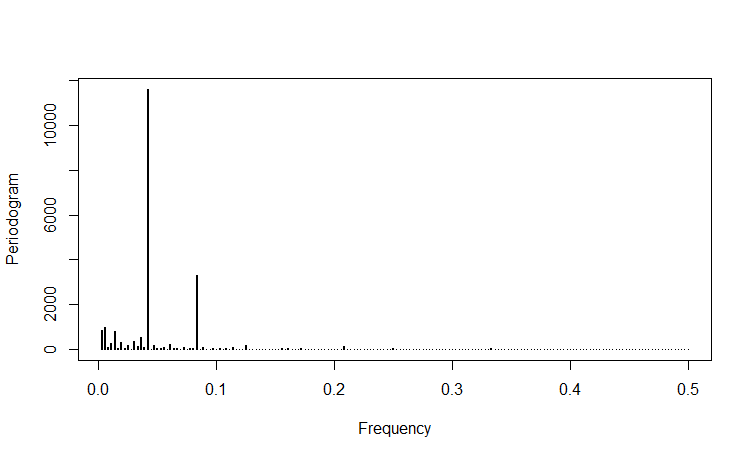
\includegraphics[width=0.8\textwidth]{figures/forecasting/periodogram_July_2014.png}
	\caption{Periodogram of hourly day ahead prices of Nord Pool Spot, Helsinki from July 7th to July 21st in 2014}
	\label{fig:periodogram_July_2014}
\end{figure}

After successfully determine meaningful seasonalities and their resulting periods from the dataset this information can be used to build forecast models that consider the respective seasonal periods in the model generation process. 



\subsection{Seasonal decomposition} \label{ssec:seasonal_decomposition}

Seasonal decomposition describes the process of decomposing a given time series into its components which are trend, seasonal or cyclic and irregular components. Decomposition is done by applying the STL model to the time series and extracting the above mentioned components where STL is defined as Seasonal-Trend decomposition procedure based on Loess \cite{cleveland1990stl}. 

The decomposition of a time series can be formalized as follows \cite{cleveland1990stl}: 

	\[ Y_v = T_v + S_v + R_v \]
	
where $Y_v$ denotes the original time series, $T_v$ the trend component, $S_v$ the seasonal component and $R_v$ the remainder component. $v \in \{ 1,\ldots,N \}$ denotes an individual time stamp in the series where $N$ is the number of unit time stamps in the time series. 

A sample seasonal decomposition of hourly time series is depicted in Figure \ref{fig:stl_decomposition_July_2014}. 

\begin{figure}[htbp]
	\centering
		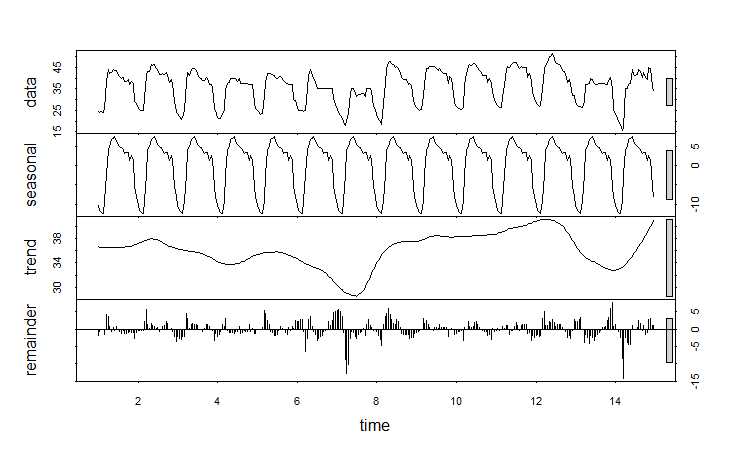
\includegraphics[width=1.00\textwidth]{figures/forecasting/stl_decomposition_July_2014.png}
	\caption{STL decomposition of hourly day ahead time series, Nord Pool Spot, Helsinki from July 7th to July 21st in 2014}	
	\label{fig:stl_decomposition_July_2014}
\end{figure}

The plot consists of four rows with each row containing a different time series component. 
The first row shows the original time series with hourly prices over a time period of two weeks. There are evident daily and weekly seasonal periods visible in the time series. Daily seasonality can be observed by the repetitive pattern of highs and lows over each day whereas weekly seasonality is evident due to the recognizable decline of prices towards the end of each week. 

The second row represents the extracted daily seasonal component which depicts the daily variation in prices. STL is only capable of extracting a single seasonality pattern. In case both daily and weekly seasonal periods should be extracted a BATS or TBATS model can be used (these models are discussed later in this section). 

In the third row the trend component is displayed. It shows a seemingly repetitive pattern over one week, which denotes the weekly seasonal period observable from the original time series. 

Finally in the last row the remaining irregular component is shown which contains all remaining variations in the time series. 

The grey bars at the right hand side of each plot aim to provide a relative comparison of scales over all plots, i.e.~the height of the bars show the same value range in different scales. Thus the whole value range of the trend component is equivalent with the value range of about one third of the original time series. 




\subsection{Forecast models}

Different statistical forecast models have been chosen to be investigated on a large scale. The selection of forecast models includes simpler models such as Simple Exponential Smoothing and more advanced models such as ARIMA and TBATS and variants thereof. The purpose of the evaluation is to provide insights into the performance of different forecast models when applied to electricity price time series. 

\subsubsection{Mean forecast}

The mean forecast is a simple model based on previous observations of a time series. It calculates the mean over a training data set and uses this mean as forecast for all future values \cite{hyndman2012forecasting}. 

It can be formally defined as in equation \ref{eq:mean_forecast}

%\begin{equation}
%\hat{Y}_{t+i} = Y_t
%\label{eq:naive_forecast}
%\end{equation}

\begin{equation}
\hat{y}_{T+h|T} = \frac{1}{T} \sum_{i=1}^T y_i
\label{eq:mean_forecast}
\end{equation}

where $T$ denotes the number of observations in the trainings dataset, $y_i$ denote historical values and $\hat{y}_{T+h|T}$ denotes a forecast of $h$ values into the future beginning at the value of $y_T$. 

Even though the mean forecast only includes simple calculations it can be effective to forecast random or near random time series or time series that exhibit strong volatility. As it is the simplest of the proposed models it should serve as a baseline model to which other models' performance can be compared. 

\subsubsection{Simple Exponential Smoothing}

The Simple Exponential Smoothing model (SES) belongs to the category of exponential smoothing models which calculate the weighted average over historical observations where weights are exponentially decreased for observations in the past. 

As the name implies this model is the simplest of exponential smoothing models which is designed to provide forecast for time series without trend or seasonal components. Similar to the mean forecast model past values of a time series are processed but with given weights that decrease exponentially over time \cite{hyndman2012forecasting,weron2007modeling}. 

The corresponding formula is depicted in Equation \ref{eq:ses_forecast} 

\begin{equation}
\hat{y}_{T+1|T} = \sum_{i=0}^{T-1} \alpha (1 - \alpha)^i y_{T-i}
\label{eq:ses_forecast}
\end{equation}

where $\alpha$ with $0 \le \alpha \le 1$ denotes the smoothing parameter that determines the influence of past observations through setting the corresponding weights. Thus by modifying values of $\alpha$ the resulting impact of past values to forecasted values can be defined. 

\subsubsection{Holt's Exponential Smoothing}

Holt's Exponential Smoothing (Holt's ES) is a linear trend method which extends Simple Exponential Smoothing by including trends in the model generation process \cite{hyndman2012forecasting}. The model consists of two separately modeled components which are level and trend components. These are combined to obtain forecasts for a given time series. It can be formalized by the following equations:

\begin{align}
 \hat{y}_{t+h|t} &= l_t + h b_t \label{eq:holts_forecast} \\
 l_t &= \alpha y_t + (1 - \alpha) (l_{t-1} + b_{t-1})\label{eq:holts_level_component} \\
 b_t &= \beta (l_t - l_{t-1}) + (1 - \beta) b_{t-1}\label{eq:holts_trend_component}
\end{align}

Equation \ref{eq:holts_forecast} denotes the forecast value $\hat{y}_{t+h|t}$ which is forecasted $h$ steps into the future beginning from time stamp $t$. It consists of a combination of the level $l_t$ at time $t$ and the trend $b_t$ at time $t$ continued over the next $h$ time intervals. 

The level component is described in Equation \ref{eq:holts_level_component} which denotes a linear combination of the actual value $y_t$ at time $t$ and the level forecast constructed from previous time stamp's level $l_{t-1}$ and trend $b_{t-1}$ components. 

Equation \ref{eq:holts_trend_component} depicts the trend component which is a linear combination of the difference of the current and previous levels ($l_t, l_{t-1}$) and the estimated trend component $b_{t-1}$ from the previous point in time. 

$\alpha$ and $\beta$ exhibit characteristics $0 \le \alpha \le 1$ and $0 \le \beta \le 1$ and denote the smoothing parameters for the level and trend components, respectively.

\subsubsection{Seasonal HoltWinter's model}

The Seasonal HoltWinter's model is the first of the discussed models which is capable of modeling seasonality in the dataset. It further extends the capabilities of the SES and Holt's ES models by an additional seasonal component. Thus besides the level and trend components $l_t$ and $b_t$ a seasonal component $s_t$ is introduced, with smoothing parameters $\alpha, \beta, \gamma$, respectively \cite{hyndman2012forecasting}. 

The corresponding equations are defined as

\begin{align}
 \hat{y}_{t+h|t} &= l_t + h b_t + s_{t-m+h_m^+} \label{eq:holtwinter_forecast} \\
 l_t &= \alpha (y_t - s_{t-m}) + (1 - \alpha) (l_{t-1} + b_{t-1})\label{eq:holtwinter_forecast_level_component} \\
 b_t &= \beta (l_t - l_{t-1}) + (1 - \beta) b_{t-1}\label{eq:holtwinter_forecast_trend_component} \\
 s_t &= \gamma (y_t - l_{t-1} - b_{t-1}) + (1 - \gamma) s_{t-m}\label{eq:holtwinter_forecast_seasonal_component}
\end{align}

where $m$ denotes the period of seasonality (e.g.~$m=12$ for monthly data when one year is the base unit) and $h_m^+ = \left\lfloor (h-1) \mod m\right\rfloor + 1$ represents the additional number of steps ahead required to model the corresponding seasonal period $m$. Therefore $s_{t-m+h_m^+}$ denotes the previously occurred seasonal period which is added to the forecast equation in Equation \ref{eq:holtwinter_forecast}. 

The level component in Equation \ref{eq:holtwinter_forecast_level_component} is adjusted by the level of the last occurred seasonal period $s_{t-m}$ to consider seasonal differences. The equation for the trend component $b_t$ is taken directly from the one of Holt's ES in Equation \ref{eq:holts_trend_component} whereas the seasonal component is defined in Equation \ref{eq:holtwinter_forecast_seasonal_component}. 

The seasonal component is denoted as a weighted sum of the current value $y_t$ substracted by previous level and trend components and the value of the seasonal component exactly $m$ periods before. 

The smoothing parameters $\alpha, \beta$ and $\gamma$ are estimated by minimizing the squared one-step prediction error to appropriately weigh the different components to yield best results \cite{r2016language}. 


\subsubsection{ARIMA models}

ARIMA models or Auto Regressive Integrated Moving Average models are highly adjustable time series models that can incorporate a number of features from the dataset. They are capable of modeling correlations in the data as well as provide a smoothing method to dampen the impact of extreme outliers. 

ARIMA models may consist of both autoregressive (AR) and moving average (MA) terms to accurately model the underlying dataset \cite{hyndman2012forecasting,weron2007modeling}. 

\paragraph{AR model} The autoregressive component is used to model dependencies in the data such that correlations within the dataset are reduced. It is defined as a weighted sum of past values of an observation. An AR(p) model is shown in Equation \ref{eq:ar_component}.

\begin{equation}
	y_t = c + \sum_{i=1}^p \phi_i y_{t-i} + e_t
\label{eq:ar_component}
\end{equation}

where $y_t$ is modeled as the sum of the past $p$ values of $y$ plus an additional error component $e_t$ and a constant $c$. AR coefficients $\phi_1,\ldots,\phi_p$ are used to weight past observations and need to be estimated in the model generation process. 

\paragraph{MA model} The moving average component models a time series as a moving average of past error terms. Equation \ref{eq:ma_component} gives the formal definition: 

\begin{equation}
	y_t = c + e_t + \sum_{i=1}^q \theta_i e_{t-i}
\label{eq:ma_component}
\end{equation}

where $e_t$ denotes the forecast error at time $t$ and the error terms are weighted by MA coefficients $\theta_1,\ldots,\theta_q$.

\paragraph{ARIMA model} An ARIMA model consist of both AR and MA terms. In addition ARIMA models are able to model non-stationary time series by applying differencing operations to the dataset. ARIMA(p,d,q) denotes a model consisting of $p$ number of AR terms, $q$ MA terms and $d$ number of differences. 
It can be described as the sum of AR and MA terms:

\begin{equation}
	y_t = \sum_{i=1}^p \phi_i y_{t-i} + \sum_{i=1}^q \theta_i e_{t-i} + e_t + c
\label{eq:arima_model}
\end{equation}

When applying the model the possible applied differences during data preprocessing are reversed by integrating the results which refers to the \textit{Integrating} part of the model. 

ARIMA models can be enhanced to model seasonal periods which are defined as ARIMA (p,d,q)(P,D,Q)\textsubscript{m} also denoted as SARIMA models. 
In addition to non-seasonal parameters $p, d$ and $q$ the seasonal parameters $P$, $D$ and $Q$ denote the seasonal AR, differencing and MA components, respectively. 



\subsubsection{BATS and TBATS models}

Multiple seasonal periods can be applied by models such as BATS and TBATS \cite{r2016language}. This can be done by applying a BATS or TBATS model to the time series, identifying different seasonal and trend components and modeling each component separately \cite{de2011forecasting}. 

Both BATS and TBATS models are able to handle multiple seasonalities in the data, i.e.~considering both daily and weekly seasonal periods where TBATS models are capable of modeling non-integer periods as well (e.g.~365.25 for annual seasonality). 

\paragraph{BATS model} BATS stands for Box-Cox transform, ARMA errors, Trend, and Seasonal components. TBATS can then be regarded as the trigonometric version of BATS. 

The definition of BATS is outlined in the following equations: 


\begin{equation}
	y_t^{(\omega)} = 
	\begin{cases}
		\frac{y_t^\omega - 1}{\omega}, & \omega \neq 0 \\
		\log y_t, & \omega = 0
	\end{cases}
\end{equation}


%\begin{equation}
	%y_t^{(\omega)} = 
	%\begin{cases}
		%\frac{y_t^\omega - 1}{\omega}, & \text{if}\ a=1 \\
		%\log y_t, & \text{otherwise}
	%\end{cases}
%\end{equation}


\begin{align}
	y_t^{(\omega)} &= l_{t-1} + \phi b_{t-1} + \sum_{i=1}^T s_{t-m_i}^{(i)} + d_t\label{eq:bats_model} \\
	l_t &= l_{t-1} + \phi b_{t-1} + \alpha d_t \\
	b_t &= (1 - \phi) b + \phi b_{t-1} + \beta d_t \\
	s_t^{(i)} &= s_{t-m_i}^{(i)} + \gamma_i d_t\label{eq:bats_seasonal} \\
	d_t &= \sum_{i=1}^p \Phi_i d_{t-i} + \sum_{i=1}^q \theta_i e_{t-i} + e_t
\end{align}

where $y_t^{(\omega)}$ denotes the Box-Cox transformed value with parameter $\omega$ where $y_t$ is the current value at time $t$ (See also Box-Cox transform in \ref{ssec:box_cox_transformation}). 

$l_t$ describes the level, $b$ denotes the long term trend, $b_t$ represents the trend, $e_t$ is gaussian white noise with zero mean and constant variance and $s_t^{(i)}$ denotes the i-th seasonal component. $\phi$ denotes the damping parameter for the trend and defines the impact of short and long term trends. All of these components are adjusted by a weighted ARMA component $d_t$ and coefficients $\alpha$, $\beta$ and $\gamma$, respectively. 

A BATS model is parameterized by BATS($\omega$,$\phi$,$p$,$q$,$m_1$,\ldots,$m_T$) with the Box-Cox parameter $\omega$, damping parameter $\phi$, ARMA parameters $p$ and $q$ and seasonal periods $m_1,\ldots,m_T$. A double seasonal model (e.g.~daily and weekly) with an AR(1) component can be described as BATS(1,1,1,0,$m_1$,$m_2$) with default Box-Cox and damping parameters. 

\paragraph{TBATS model} As BATS models possibly result in a large number of states and only pure integer seasonal periods may be modeled, the TBATS model has been developed \cite{de2011forecasting}. This model enhances the BATS model with trigonometric expressions:

\begin{align}
	s_t^{(i)} &= \sum_{j=1}^{k_i} s_{j,t}^{(i)}\label{eq:tbats_seasonal} \\
	s_{j,t}^{(i)} &= s_{j,t-1}^{(i)} \cos \lambda_j^{(i)} + s_{j,t-1}^{*(i)} \sin \lambda_j^{(i)} + \gamma_1^{(i)} d_t \\
	s_{j,t}^{*(i)} &= - s_{j,t-1} \sin \lambda_j^{(i)} + s_{j,t-1}^{*(i)} \cos \lambda_j^{(i)} + \gamma_2^{(i)} d_t 
\end{align}

where $s_{j,t}^{(i)}$ describes the stochastic level of the i-th seasonal component and $s_{j,t}^{*(i)}$ represents the stochastic growth in the level of the i-th seasonal component which can be described as the change of value of the seasonal component over a period of time. $k_i$ is the number of harmonics required for the ith seasonal component, $\gamma_1^{(i)}$ and $\gamma_2^{(i)}$ are smoothing parameters and $\lambda_j^{(i)} = \frac{2 \pi j}{m_i}$ the trigonometric parameter which depends on the corresponding seasonal period $m_i$. 

Finally the model can be obtained by replacing $s_t^{(i)}$ in equation \ref{eq:bats_seasonal} by the trigonometric expression in equation \ref{eq:tbats_seasonal} and replacing $s_{t-m_i}^{(i)}$ in equation \ref{eq:bats_model} by $s_{t-1}^{(i)}$. 


\subsection{Box Cox transformation} \label{ssec:box_cox_transformation}

Box cox transformations are used to transform non-normal data to exhibit a normal distribution like behavior \cite{box1964analysis}. Since most statistical time series models (e.g.~ARIMA) require data to have constant variance this technique can be used as a preprocessing step before applying data to forecasting models \cite{nelson1979experience}. 

The formula for box cox transformations is as follows: 


\begin{equation}
	y^{(\lambda)} = 
	\begin{cases}
		\frac{y^\lambda - 1}{\lambda}, & \lambda \neq 0 \\
		\log y, & \lambda = 0
	\end{cases}
	\label{eq:box_cox_transform}
\end{equation}

\begin{equation}
	y^{(\lambda)} = 
	\begin{cases}
		\frac{(y + c)^\lambda - 1}{\lambda}, & \lambda \neq 0 \\
		\log (y + c), & \lambda = 0
	\end{cases}
	\label{eq:box_cox_transform_with_constant}
\end{equation}

where conditions $y > 0$ and $y > -c$ apply to equations \ref{eq:box_cox_transform} and \ref{eq:box_cox_transform_with_constant}, respectively. 

Since the value of $\lambda$ can be less than one $y$ has to be positive and thus a constant term $c > 0$ is required in case $y < 0$ (equation  \ref{eq:box_cox_transform_with_constant}). 

In \cite{nelson1979experience} the autors show that it might not be always possible to transform a series to show a normal distribution and that the application of the procedure can be costly. Still some improvements to forecasts can be achieved by applying Box-Cox transformation to non-normal distributions as a preprocessing step to model generation. 


\subsection{Forecast accuracy measures} \label{ssec:forecast_acc_measures}

Different forecast accuracy methods can be applied to investigate model performance. These methods are based on estimating the overall forecast error for a given model and forecast horizon \cite{hyndman2012forecasting, weron2007modeling}. 

The forecast errors are computed as a function of residuals which are defined as the differences of actual values to forecasts \cite{hyndman2012forecasting}: 

\begin{equation}
	e_i = y_i - \hat{y_i}
\label{eq:residuals}
\end{equation}

where $\hat{y_t}$ denotes the one step ahead forecast based on a series of past values $\{y_1,\ldots,y_{t-1}\}$. 


\subsubsection{Scale-dependent error measures}

Scale dependent errors are absolute error measures depending on the scale of the examined dataset. Therefore when comparing these types of error measures they should be applied to data showing the same scale. 

\paragraph{Mean error}
The mean error (ME) denotes a measure of the mean value of forecast errors over a given period of time. 
It can be seen as indication of the symmetry of the forecast error distribution. 

\begin{equation}
\frac{1}{n} \sum_{i=1}^{n} \hat{y}_i - y_i
\label{eq:acc_me}
\end{equation}

where $n$ is the number of observations, $\hat{y}_i$ is the forecast for observation $i$ and $y_i$ denotes the actual value for observation $i$. 

\paragraph{Mean absolute error}
The mean absolute error (MAE) shows the mean of all absolute errors over the forecast horizon where the absolute error is defined by the absolute difference between a value of the dataset and its forecasted value. The mean absolute error provides a means for retrieving a measure proportional to actual forecast errors. 

\begin{equation}
\frac{1}{n} \sum_{i=1}^{n} |\hat{y}_i - y_i|
\label{eq:acc_mae}
\end{equation}



\paragraph{Root mean squared error}
The root mean squared error (RMSE) takes the root of the sum of the squared forecast errors which puts more emphasis on possible outliers in residual values. 

\begin{equation}
	\sqrt{\frac{1}{n} \sum_{i=1}^{n} (\hat{y}_i - y_i)^2}
\label{eq:acc_rmse}
\end{equation}


\subsubsection{Percentage based error measures}

Percentage based error measures have the advantage of providing scale independent measures for comparing forecast errors across different time series. However a significant disadvantage of percentage errors is their inability to handle zero values in time series. Also numerical compuations become unstable when values get closer to zero. 


\paragraph{Mean percentage error}

The mean percentage error (MPE) is dependent on the symmetry of the forecast error distribution as positive and negative value differences might cancel each other out. This can be compared to the mean error which shows the same behavior as a scale dependent measure. 


\begin{equation}
\frac{1}{n} \sum_{i=1}^{n} \frac{\hat{y}_i - y_i}{y_i}
\label{eq:acc_mpe}
\end{equation}



\paragraph{Mean absolute percentage error}

The mean absolute percentage error (MAPE) shows similar to the mean absolute error the mean of all absolute errors but as percentage error relative to the corresponding actual value. 

\begin{equation}
\frac{1}{n} \sum_{i=1}^{n} \left|\frac{\hat{y}_i - y_i}{y_i}\right|
\label{eq:acc_mape}
\end{equation}




\section{Model generation} \label{sec:model_generation}

In this section the procedure of generating an ARIMA model is described. Since ARIMA models are classical time series models which showed reasonable results in energy price forecasting \cite{aggarwal2009electricity,weron2005forecasting} they have been investigated in detail to provide a better understanding of the model generation process. 

In addition to the well known Box Jenkins approach (see section \ref{ssec:arima_models_to_predict_next_day_prices}) a custom model selection process is proposed for manual ARIMA model selection \cite{hyndman2012forecasting}. This process is outlined in Figure \ref{fig:manual_arima_forecasting_procedure}.

\begin{figure}[htbp]
	\centering
		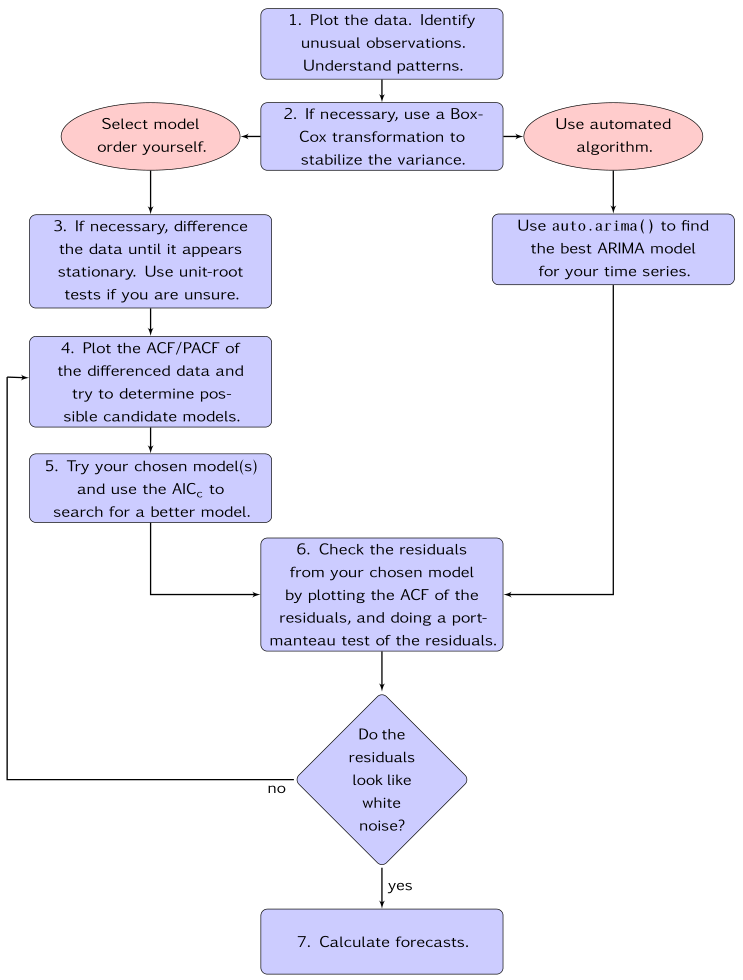
\includegraphics[width=0.70\textwidth]{figures/forecasting/manual_arima_forecasting_procedure.png}
	\caption{Manual ARIMA model generation process \cite{hyndman2012forecasting}}
	\label{fig:manual_arima_forecasting_procedure}
\end{figure}

In this case a manual model generation process is conducted. The data based on which a model will be generated together with diagnostic plots (ACF, PACF) is shown in Figure \ref{fig:tsdiag_prices_acf_pacf}. 

\begin{figure}[htbp]
	\centering
		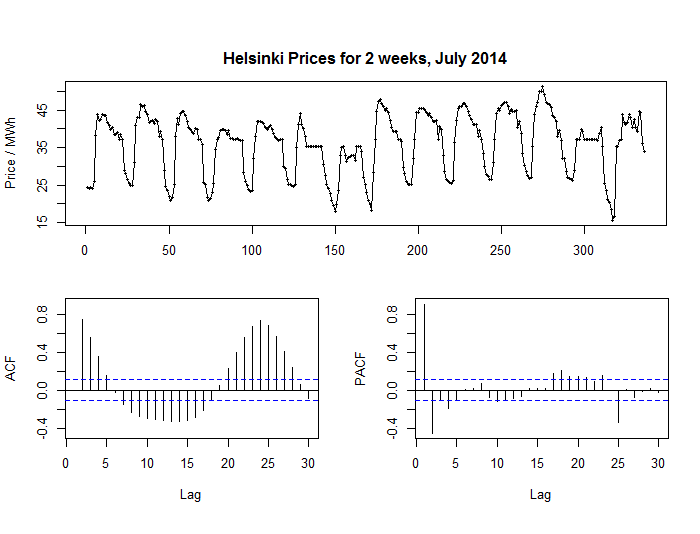
\includegraphics[width=0.95\textwidth]{figures/forecasting/tsdiag_prices_acf_pacf.png}
	\caption{Two weeks of hourly day ahead prices with ACF and PACF plots (Nord Pool Spot, Helsinki from July 7th to July 21st in 2014)}
	\label{fig:tsdiag_prices_acf_pacf}
\end{figure}

The dataset consists of two weeks of hourly day ahead prices amounting to a total of 336 hours. Figure \ref{fig:tsdiag_prices_acf_pacf} shows three plots, at the top a time series plot showing the energy price time series is depicted, on the bottom left an autocorrelation plot (ACF) is shown and on the bottom right a partial autocorrelation plot (PACF) is printed. 
As already discussed in section \ref{ssec:seasonal_decomposition} this data exhibits daily and weekly seasonality which is clearly visible on the time series plot. 

As ARIMA models require data to be stationary (i.e.~it exhibits no trend or seasonality) the proposed method to transform a series into a stationary series is to apply one or more levels of differencing or seasonal differencing. The resulting residuals of the model should show no autocorrelations and should exhibit a zero mean \cite{hyndman2012forecasting}. Ideally residuals have constant variance and exhibit a normal distribution as well. 

ACF and PACF plots are diagnostic plots to examine correlations within the dataset \cite{nist2012handbook,nau2016statistical}. 
Both ACF and PACF plots display individual lags on the x-coordinate while on the y-coordinate the values of the autocorrelation and partial autocorrelation functions are displayed for ACF and PACF plots, respectively. The dashed blue lines denote the 95\% confidence interval for white noise, i.e.~lag values contained within this interval do not reject the white noise hypothesis. 
Values exceeding the confidence bounds are "`significant"' regarding correlations in the data. 
%However 1 in 20 lags is allowed to exceed the significance bounds without violating the white noise assumption. 

The ACF plot displays the ``coefficients of correlation between a time series and lags of itself'' whereas the PACF plot shows the ``partial correlation coefficients between the series and lags of itself'' \cite{nau2016statistical}. 
Correlation coefficients for autocorrelations are said to be interdependent which means that the value of an autocorrelation at lag $h$ depends on correlations of all previous lags $1,\ldots,h-1$. In contrast, partial autocorrelations only include correlations specific to lag $h$ without considering correlations at lower order lags. 

According to the model generation process in Figure \ref{fig:manual_arima_forecasting_procedure} data should be differenced if necessary to make the series stationary. In this case a seasonal difference might be appropriate due to the obvious seasonality in the time series. 

The ACF plot above shows a decay of significant autocorrelations whereas the PACF plot depicts several significant spikes with most significant ones at lags 2 and 25. 
As the spike at lag 25 in the PACF plot is close to the assumed seasonal period of 24 this may suggest adding a seasonal AR(1) term with a period of 24. The peak value at lag 24 in the ACF plot may be another indicator of seasonal correlation.
Therefore, the suggested intermediate ARIMA model is ARIMA(0,0,0)(1,1,0)[24] with a seasonal AR term and one level of seasonal differencing with a period of 24. 

The resulting model residuals are depicted in Figure \ref{fig:residuals_arima_000_110}. 

\begin{figure}[htbp]
	\centering
		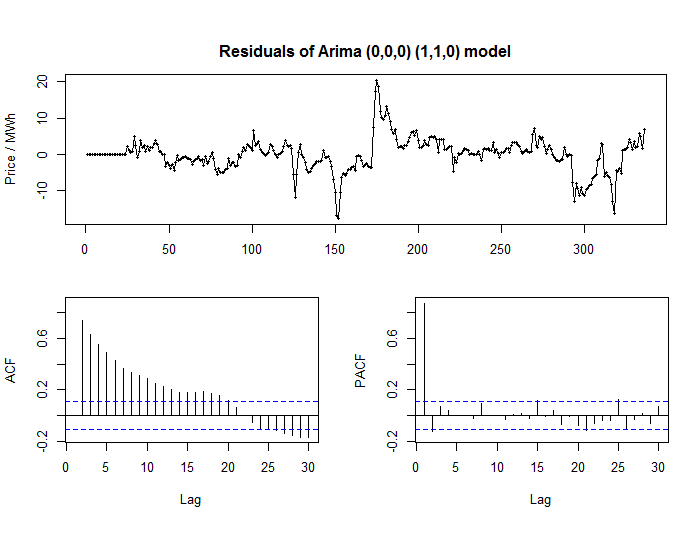
\includegraphics[width=0.95\textwidth]{figures/forecasting/residuals_arima_000_110.png}
	\caption{Intermediate ARIMA(0,0,0)(1,1,0)[24] model with seasonal difference}
	\label{fig:residuals_arima_000_110}
\end{figure}

Figure \ref{fig:residuals_arima_000_110} depicts residuals with removed hourly seasonality and zero mean. However the series can not be regarded as stationary as significant deviations exist from the mean in the time series. Apart from the weekly seasonality further correlations can be identified. 

According to \cite{nau2016statistical} a cut-off (rapid decrease of correlation values) at the PACF plot indicates adding an AR term with an order corresponding to the number of the last significant lag of this occurrence. Conversely a cut-off at the ACF plot indicates the addition of a MA term with the number of the last significant lag in the ACF plot. 

Since Figure \ref{fig:residuals_arima_000_110} shows a slow decay in the ACF and a small but significant coefficient at lag 2 in the PACF we recognize a cut-off at this lag in the PACF and add a (non-seasonal) AR(2) term to the model. 
Thus the resulting model is ARIMA(2,0,0)(1,1,0)[24] which is shown in Figure \ref{fig:residuals_arima_200_110}. 

\begin{figure}[htbp]
	\centering
		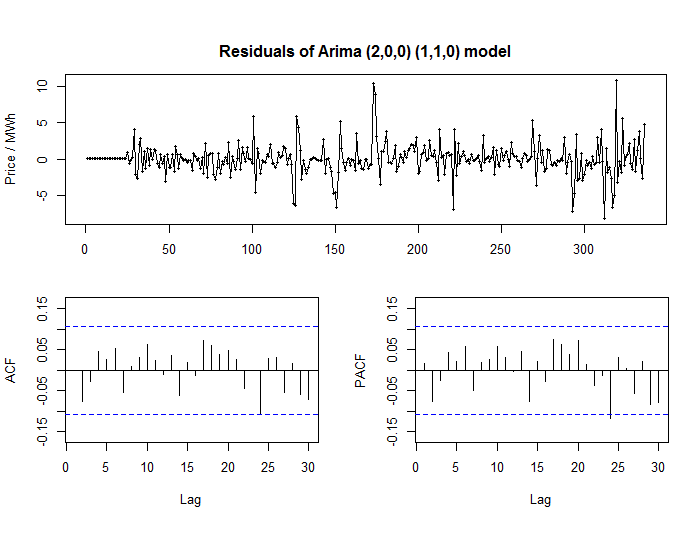
\includegraphics[width=0.95\textwidth]{figures/forecasting/residuals_arima_200_110.png}
	\caption{Residuals of ARIMA(2,0,0)(1,1,0)[24]}
	\label{fig:residuals_arima_200_110}
\end{figure}

The time series of residuals above can be assumed to be stationary as no significant deviations from the mean are visible. 

There is only one significant spike at lag 24 remaining which might indicate still some seasonal information in the data, however it could be as well regarded as outlier as 1 in 20 spikes is said to be significant by chance alone \cite{hyndman2012forecasting}. 


%
%The autocorrelation function determines the existence or non-existence of correlation between lagged variables within a time series \cite{nist2012handbook}. 
%That is, the correlation between a point in the time series to another point in the same time series is calculated where the gap between the two points is fixed by the given lag (hence the name \textit{auto}-correlation). 
%
%The autocorrelation function is defined as the autocorrelation coefficient $R_h$ (equation \ref{eq:autocorr_coeff})
%
%\begin{equation}
%R_h = \frac{C_h}{C_0}
%\label{eq:autocorr_coeff}
%\end{equation}
%
%
%where $C_h$ denotes the autocovariance function and $C_0$ defines the variance function 
%(see equations \ref{eq:autocov_func} and \ref{eq:variance_func}). 
%
%
%\begin{equation}
%C_h = \frac{1}{N} \sum\limits_{t=1}^{N-h} (Y_t - \bar{Y}) (Y_{t+h} - \bar{Y})
%\label{eq:autocov_func}
%\end{equation}
%
%
%\begin{equation}
%C_0 = \frac{1}{N} \sum\limits_{t=1}^{N} (Y_t - \bar{Y})^2
%\label{eq:variance_func}
%\end{equation}
%
%with $\bar{Y}$ denoting the mean of the series, $N$ defines the sample size, $Y_t$ the observation at time $t$ and $Y_{t+h}$ the observation $h$ steps ahead from $t$. 
%The autocovariance function determines the mean of covariance between variables with fixed lag $h$ while the variance function determines the mean variance over all timestamps $N$. 



\subsection{Model validation}



The corrected Akaike Information Criterion (AICc) is a well known goodness of fit measure for stochastic models \cite{weron2007modeling}. It provides a relative quality measure for models such that models with lower AICc values are assumed to better capture the characteristics of the underlying data. 
Equation \ref{eq:aicc_test} defines the metric. 

\begin{equation}
	AICc = -2 \log \mathcal{L} + \frac{2dn}{n - d - 1}
\label{eq:aicc_test}
\end{equation}

with $\log \mathcal{L}$ being the log-likelihood, $d$ the model size (number of parameters) and $n$ denotes the sample size. Note that the model size $d$ is present in order to penalize models having too many parameters. The log-likelihood function estimates how well the model fits the data. 

After a model has been chosen by evaluating the AICc value the model residuals should be checked for existing correlations. As shown in the last section this can be done by verifying the ACF and PACF plots but tests are available for automated testing against randomness \cite{weron2007modeling,hyndman2012forecasting}. 

One of these tests is the Ljung Box test which tests a given number of autocorrelations if they fall outside the significance bounds \cite{weron2007modeling}. The test is defined in Equation \ref{eq:ljung_box_test}. 

%for probability of showing non-white noise properties 
\begin{equation}
	Q = n(n + 2) \sum_{j=1}^{h} \frac{\hat{\rho}^2 (j)}{n - j}
\label{eq:ljung_box_test}
\end{equation}

with $n$ as the sample size, $h$ as number of lags and $\hat{\rho}^2 (j)$ as the squared autocorrelation at lag $j$. 
Its distribution can be approximated by the $\chi^2$ distribution with $h$ degrees of freedom. The white noise hypothesis is rejected if $Q > \chi_{1-\alpha}^2 (h)$ with a defined significance level $\alpha$ with $\chi_{1-\alpha}^2$ being the $(1 - \alpha)$ quantile of the $\chi^2$ distribution with $h$ degrees of freedom. 


\subsection{Model evaluation} \label{ssec:model_evaluation}

In order to assess the quality and goodness of fit of the models generated in section \ref{sec:model_generation} they are validated and compared to a model generated by an automatic model generation procedure. 

In addition to the manual model selection procedure shown in the last section automatic model generation procedures exist to detect the model with best goodness of fit parameters by iterating over a set of candidate models. 

For generating ARIMA models the \textit{auto.arima} function may be used \cite{hyndman2012forecasting,r2016language}. 

It is defined by the following steps \cite{hyndman2012forecasting}: 

\begin{enumerate}
	\item Determine the number of differences $d$ by applying a unit root test (e.g.~KPSS test).
	\item A set of candidate models is generated starting with the following models: 
				
				ARIMA(2,d,2) \\
				ARIMA(0,d,0) \\
				ARIMA(1,d,0) \\
				ARIMA(0,d,1) 
				
				Model parameters $p$ and $q$ are modified by adding $\pm 1$ where the best model is set as reference. 
				Repeat the last line until no model with a lower AICc value can be found. 

\end{enumerate}

A model has been generated using auto.arima based on the same data as used for manual model selection in section \ref{sec:model_generation}. 
The resulting models with corresponding model parameters are outlined in table \ref{tab:model_names_and_parameters}. 

\begin{table}[ht]
\centering
\begin{tabular}{l|l}
 Model Name & Model Parameters \\ 
  \hline
	Intermediate Model	& ARIMA(0,0,0)(1,1,0)[24] \\ 
	Final Model 				& ARIMA(2,0,0)(1,1,0)[24] \\ 
	Automatic Model 		& ARIMA(2,0,3)(1,0,2)[24] \\ 
\end{tabular}
\caption{Model names and parameters}
\label{tab:model_names_and_parameters}
\end{table}

AICc and Ljung Box values have been calculated for each model defined above. For Ljung Box tests a 95\% confidence interval has been used
such that resulting p-values greater than 0.05 indicate white noise properties of the residuals. Thus a high Ljung Box test value gives 
high probability of a series resembling white noise. 

The AICc and Ljung Box values are outlined in table \ref{tab:model_aicc_and_ljung_box_values}. 

\begin{table}[ht]
\centering
\begin{tabular}{r|r|r|r}
 & Intermediate Model & Final Model & Automatic Model \\ 
  \hline
	AICc 			& 1868.01 & \textbf{1400.22} & 1457.26 \\ 
  Ljung Box & < 2.2e-16 & 0.1523 & \textbf{0.9927} \\ 
\end{tabular}
\caption{AICc and Ljung Box values}
\label{tab:model_aicc_and_ljung_box_values}
\end{table}

Results show that it is possible for manually selected models to outperform automatically generated models, i.e.~the Final Model shows a lower AICc value than the Automatic Model. This is presumably due to the manual model using explicit seasonal differencing which the automatic nodel does not use. However the Ljung Box test values indicate a different result where the Automatic Model results in a higher p-value and thus exhibits less correlations than the Final Model. As both models exceed the significance bounds of 0.05 this is only of minor importance as both exhibit white noise characteristics. If in doubt the AICc value should be given precedence over Ljung Box test results. 

\section{Model selection algorithm} \label{sec:model_selection_algorithm}

An automated model selection algorithm has been implemented to provide aid in finding suitable ARIMA models for a given trainings dataset. 
The process consists of several data preprocessing steps with generation and comparison of different ARIMA models and model evaluation based on a weighted function of AICc and Ljung Box test values. 

The model selection algorithm consists of three separate functions each contributing a different part to model generation. These functions are \textit{GenerateArimaModel} as the base function for model generation, \textit{AutomatedBoxTest} for determining the right parameters for the Ljung Box tests and \textit{SeasonalPeriods} for estimation of possibly existing seasonal periods within the data. 

%They will be referred to each other as soon as they are called. 

\subsection{Function GenerateArimaModel}

\begin{enumerate}
	\item Get trainingsdata
	
	\begin{enumerate}
		\item Read time series of energy prices from given location
		\item Define trainings period by start and end date
	\end{enumerate}
	\item Determine seasonality
	
	\begin{enumerate}
		\item Call \textit{SeaonalPeriods} to retrieve seasonal periods from the data
	\end{enumerate}
	
	\item Create time series objects
	
	\begin{enumerate}
		\item For each seasonal period found create a time series object based on that period
	\end{enumerate}
	
	\item Calculate the Box-Cox transformation parameters
	
	\begin{enumerate}
		\item Compute the Box Cox parameters for each of the created time series objects
	\end{enumerate}
	
	\item Create models
	
	\begin{enumerate}
		\item Create model(s) without BoxCox transformation
		
		\begin{enumerate}
			\item Generate model with auto.arima for each of the created time series objects 
		\end{enumerate}
		
		\item Create model(s) with BoxCox transformation
		
		\begin{enumerate}
			\item Generate model with auto.arima and previously defined lambda (Box-Cox) parameter for each of the created time series objects if Box-Cox parameter is not equal to 1 (then it would have no effect)
		
		\end{enumerate}
		
	\end{enumerate}
	
	\item Execute Ljung Box test for each of the models
	
	\begin{enumerate}
		\item Call \textit{AutomatedBoxTest} to retrieve the Ljung Box p-values for each model
	\end{enumerate}
	
	\item Saving models, boxtests, AICc values and p-values in vectors
	
	\item Model Evaluation

	\begin{enumerate}
		
		\item Check model goodness of fit via AICc value comparison
		
		\begin{enumerate}
			\item $p_{aicc_i} = \frac{1}{| AIC_{min} - AIC_i | + 2}$
			%\item p_aicc = 1 / (abs(AICmin – AIC(i)) + 2)
			\item ``+2'' -> moderate the decrease of values due to the inverse function
		\end{enumerate}
		
		\item Compare p-values of Ljung Box tests to check residual characteristics
		
		\begin{enumerate}
			\item p-values range from 0 to 1 -> determine difference in relation to full range
			\item $p_{ljung} = \frac{p_{value} - 0.05}{1 - 0.05}$
		\end{enumerate}
		
	\end{enumerate}

	\item Model selection

	\begin{enumerate}
		\item Calculate weighted result based on goodness of fit values with user defined weights
		\item $F_i = w_{aicc_i} p_{aicc_i} + w_{ljung_i} p_{ljung_i}$ for each model $i \in M$
	\end{enumerate}
	
	\item Return model with the highest goodness of fit value $F_i$

\end{enumerate}


\subsection{SeasonalPeriods}

	\begin{enumerate}
		\item If target period is specified and enforced
		
		\begin{enumerate}
			\item return a list of (targetPeriod, defaultPeriod) 
		\end{enumerate}
		
		\item Else 
		
		\begin{enumerate}
			\item Get the x most frequent periods sorted by number of occurrences descending, where x is a user defined number (apply periodogram)
			\item If a max period limit has been specified, discard any periods above this limit
			\item If the number of occurrences of a period falls below the white noise threshold, discard the period
			
			\item If the target period is specified and has been found
			
			\begin{enumerate}
				\item return a list of (targetPeriod, defaultPeriod) 
			\end{enumerate}
			
			\item Otherwise
			
			\begin{enumerate}
				\item add the defaultPeriod (=1) to the list of periods and return the list
			\end{enumerate}
		\end{enumerate}
	\end{enumerate}


\subsection{AutomatedBoxTest}

\begin{enumerate}
	\item Determine the most suitable value for the lag based on the sample size and 
	whether seasonal periods are existing in the dataset. 
	
	\begin{enumerate}
		\item The following rules of thumb have been established to determine a suitable value for the lag of the test \cite{hyndman2014blog}: 
		
		\begin{enumerate}
			\item for non-seasonal time series a lag value of $h=min(10,T/5)$ should be used
			\item for seasonal time series a lag value of $h=min(2m,T/5)$ should be used,
				where $T$ denotes the sample size and $m$ the seasonal period
		\end{enumerate}
		
		\item The number of determined lags is reduced by the number of parameters in the model
		
		\item The box test is executed and result is returned
	\end{enumerate}
	
\end{enumerate}


\subsection{Discussion}

The core of the model selection algorithm are steps 8 and 9 of Function GenerateArimaModel where relative measures for both AICc and Ljung Box values have been developed to be able to integrate them into a weighted function. Thus it is possible to define weights to define the impact of each validation measure on forecast model selection. 
As mentionend before (Section \ref{ssec:model_evaluation}) AICc value results should in general be given precedence over Ljung Box values since AICc values are considered more stable. 

Another thing to note is the so called \textit{target period} in function \textit{SeasonalPeriods}. This is a user estimated period which is assumed to be contained in the dataset. If it is found it is given precedence over other periods returned. There is also the possibility of ``enforcing'' the period in which case it is taken without calculating other periods. 





\section{R / Java Simulation Framework}

The R / Java Simulation Framework is responsible for preparation and execution of a large scale simulation of generating and evaluating forecast models over an extended period of time. In this section the architecture and implementation of the simulation framework is presented as well as the interfaces existing between R and Java. 


\subsection{Architecture of the simulation framework}

The framework consists of a Java application server connected to a separately running R server on which R commands are executed. R is a statistical program which is able to model complex statistical functions and includes a considerable amount of statistical packages \cite{r2016project}. It became the de-facto standard for stochastic processing and is available free of charge as well as for various platforms. 

The Java application server has been set up as WildFly 8 \cite{red2016wildfly} with Java Enterprise Edition 7 \cite{oracle2016java} and an Oracle Database \cite{oracle2016database} which provides a scalable architecture including the possibility for modeling web service interfaces. 

In this work a collection of web services has been set up for simple access of data for external applications. This can be used e.g.~by the cloud simulator outlined in section \ref{sec:architecture_of_simulation_framework}. The Java application server wraps methods for retrieval and storage of energy price data, forecast model generation and large scale simulations. It utilizes R for complex statistical processing which is included into advanced methods for simulations and model generation. 

\subsubsection{Class diagram}

In order to visualize the most important entities of the framework a class diagram is outlined in Figure \ref{fig:EPMA_class_diagram}.

A basic entity for energy price retrieval is the \textit{Resource} which wraps the retrieved contents of an energy price source. Data retrieval happens over a generic \textit{DataFetch} interface which is able to fetch data from an URL (e.g.~web service) or directly from a file. The parsing of the energy price data is achieved by a generic \textit{Parser} interface which can be implemented by Parsers for different file types (currently XLS and CSV). 

A \textit{ResourceType} stores a reference to a specific DataFetch and Parser implementation. As source types and formats of energy data will be different for each energy market at least one DataFetch and Parser implementation has to be provided for each market. The \textit{ResourceManager} keeps track of all resources associated with a registered energy market. It is implemented by resource managers for day ahead and real time markets, respectively. 

The \textit{MarketData} entity handles all the logic necessary for actually retrieving energy price data for a given Resource. It provides methods to retrieve data from registered energy sources and subsequently parsing and importing the data into the database. Instances of MarketData are used by \textit{RTPricesResourceRESTService} and \textit{DAPricesResourceRESTService} that provide web service interfaces for data retrieval. In turn, \textit{RManagerResourceRESTService} utilizes these web services to retrieve energy price data for model generation and forecast simulations. 

\begin{figure}[htbp]
	% used to position the image at the horizontal center of the page
	\hspace*{0.5in}
		% include the graphic rotated by a 90 degree angle and scale to paperwidth and height
		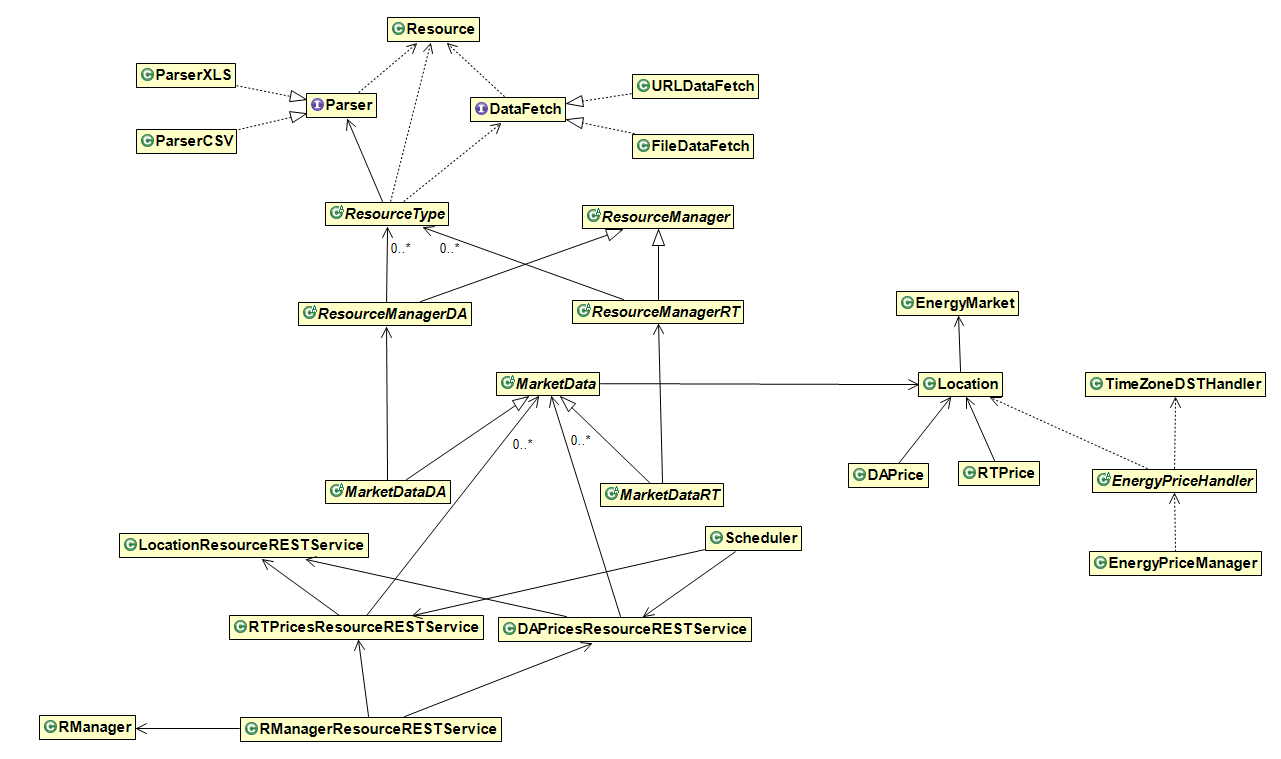
\includegraphics[angle=90,width=\paperheight,height=\paperwidth,keepaspectratio=true]{figures/forecasting/EPMA_class_diagram.png}
	\caption{Class diagram of Energy Price Management Application}
	\label{fig:EPMA_class_diagram}
\end{figure}

The \textit{Scheduler} utilizes Java EE scheduling mechanisms to automatically retrieve energy prices from specific locations at defined time intervals (e.g.~each day at 3 pm). Thus for continuous operation a scheduler can be set up for a location and dates when data should be retrieved regularly from defined interfaces. 

Each MarketData instance stores a reference to a specific \textit{Location} of an \textit{EnergyMarket}. Instances of \textit{DAPrice} and \textit{RTPrice} reference the location from which they were retrieved where these price entities each resemble exactly one energy price entity stored in the database.

Finally the \textit{EnergyPriceHandler} provides a generic interface for parsing energy prices with location specific DST (daylight saving time) changes. This interface is extended by specific implementations of energy markets to manage DST dates. The \textit{TimeZoneDSTHandler} provides a method to retrieve exact DST dates for each location and year. Thus energy prices are stored with dates correctly considering DST changes specific to each location. 

\subsubsection{Web Service interfaces}

The \textit{Energy Price Management Application} (EPMA) on the application server provides different types of web service interfaces. 

Web services are grouped by type: 
%i.e.~management of day ahead prices, real time prices, locations, energy markets and R resources corresponding to classes 

\begin{itemize}
	\item \textit{DAPricesResourceRESTService} for managing day ahead prices
	\item \textit{RTPricesResourceRESTService} for managing real time prices
	\item \textit{LocationResourceRESTService} for managing locations
	\item \textit{EnergyMarketResourceRESTService} for managing energy markets
	\item \textit{RManagerResourceRESTService} for managing R resources
\end{itemize}

Each web service interface is defined by a base path (e.g.~/rtprices), the respective web service name (e.g.~/importall) and mandatory or optional web service parameters. 

%idea: list of all web service methods in the appendix
%
%provide tables with following structure: 
%basepath	web service name		mandatory parameters			optional parameters


%\subsubsection{Energy price data retrieval}



\subsection{R Forecast evaluation}

%fcHorizons <- c("1h","3h","6h","12h","18h","24h","36h","48h","96h","168h")
%accMeasures <- c("ME","RMSE","MAE","MPE","MAPE")
%modelNames <- c("mean","ses","holts","holtwinters","arima","tbats")

The forecast model evaluation discussed in Section \ref{sec:forecast_model_evaluation} is based on implementation of an R function which is called and processed by respective methods on the application server. 

The corresponding R function is named \textit{evaluateModels} and takes energy price data as input separated into a trainings and test data sets. It generates different forecast models based on the given trainings set considering possible seasonal periods in the data (see Section \ref{sec:model_selection_algorithm}) and returns aggregated accuracy measures for each model and forecast horizon. 

\subsubsection{Function evaluateModels}

\begin{tabular}{ll}
\textbf{Input:}  & \textit{pricesTraining} - a list of energy prices taken as trainings data set \\
								 & \textit{pricesTest} - a list of energy prices taken as test data set \\
\textbf{Output:} & \textit{modelList} - a list of models generated within the function \\
								 & \textit{accuracyList} - a list of accuracy measures calculated for each model
\end{tabular}


\begin{lstlisting}[language=R, caption=Function evaluateModels, label={lst:evaluateModelsR}]
evaluateModels <- function(pricesTraining, pricesTest)
{
  period <- getSeasonalPeriod()
  pricesTrainingTs <- generateTimeSeries(pricesTraining, period)
  modelList <- generateModels(Mean,Ses,Holt,HoltWinters, 
	                              Arima,Tbats)						
  accuracyList <- list()
  forecastHorizonList <- (1,3,6,12,18,24,36,48,96,168)
  for( m in modelList ) {
    for( h in forecastHorizonList ) {
      fc <- getForecastForHorizon(m,h)
      accuracyList(m,h) <- getAccuracyMeasures(fc,pricesTest)
    }
  }
  return list(modelList,accuracyList)
}
\end{lstlisting}

In Listing \ref{lst:evaluateModelsR} the function \textit{evaluateModels} is defined. In lines 3 and 4 the most prevailing seasonal period (if any) is determined and 
a time series object is generated based on that period. In line 5 a series of forecast models is generated that are investigated in the algorithm which are Mean forecast model, SES model, Holt (SES with trend), HoltWinters (SES with trend and seasonality), ARIMA (model generation described in Section \ref{sec:model_generation}) and TBATS (seasonal model). 

Line 8 sets a list of forecast horizons in hours, i.e.~forecasts are generated for horizons from 1 up to 168 hours. In line 11 forecasts are produced for each model and forecast horizon separately and in line 12 the generated forecasts are validated by getting accuracy measures for out-of-sample forecasts based on the test data set. 
Line 15 returns a compound object of the list of generated models and accuracy measures. 



\subsection{Java implementation on application server} \label{ssec:java_implementation_on_application_server}

A large scale evaluation of forecasting methods should be conducted where models and corresponding accuracy measures are generated for different training data sets over an extended period of time. 
Thus the application server implements methods for performing customizable forecasting simulations. 

A java method \textit{evaluateModels} in class \textit{RManager} has been implemented which calls the previously introduced R function \textit{evaluateModels} (Listing \ref{lst:evaluateModelsR}) and saves the result in an internal folder on the application server. 
This method is in turn called by an identically named method in \textit{RManagerResourceRESTService} which provides the REST service interfaces to external applications for retrieval of results. 

In order to conduct automated large scale simulations additional methods have been implemented in \textit{RManagerResourceRESTService} to perform customizable simulations. The method \textit{runSimulation} performs a simulation based on a number of parameters. The method signature is depicted in Listing \ref{lst:runSimulation}. 

\begin{minipage}{\linewidth}
\begin{lstlisting}[language=Java, caption=Method runSimulation, label={lst:runSimulation}]
runSimulation(String priceType, Long locationId, 
              String simulationStart, String simulationEnd,
              String trainingsPeriod, String testPeriod, String intervalPeriod)
\end{lstlisting}
\end{minipage}

The \textit{priceType} defines whether the simulation should be based on day ahead or real time prices. Accordingly the parameter is set to either ``da'' or ``rt''. The \textit{locationId} expects an Id of a registered location within the application server. The parameter \textit{simulationStart} expects a date time String containing the start date from where the simulation should be started. The parameter \textit{simulationEnd} describes the end date of the simulation as a date time String, respectively. \textit{trainingsPeriod} is the trainings period for which energy prices should be loaded for model generation, \textit{testPeriod} is the test period against which the models are to be tested and \textit{intervalPeriod} denotes the time interval the simulation should be advanced in each step. 

The corresponding web service interface is given in Listing \ref{lst:runSimulationWebService}. 

\begin{minipage}{\linewidth}
\begin{lstlisting}[language=Java, caption=Method runSimulation web service interface, label={lst:runSimulationWebService}]
/r/simulation/{type}/{loc_id}/{simulationStart}/{simulationEnd}/
                {trainingsPeriod}/{testPeriod}/{intervalPeriod}
\end{lstlisting}
\end{minipage}

The base path of the web service interface is \textit{/r} which is an indicator for web services that are based on R implementations. The name of the web service is \textit{simulation} and parameters have already been described for Listing \ref{lst:runSimulation}. This method or interface is responsible for executing a single simulation with defined start and end dates, trainings-, test- and interval periods. 

A common format has been defined to distinguish different periods and intervals. A regular expression for the format could be described as \textit{\textasciicircum\textbackslash d+[hdw]\$}
which is a combination of at least one digit and one of \textit{h}, \textit{d} or \textit{w} which means \textit{hour}, \textit{day} and \textit{week}, respectively. 
Therefore a trainings period of 2w, 1d or 48h means two weeks, one day or 48 hours. The same holds true for test- and interval periods. 

The method \textit{runSimulation} calls the method \textit{evaluateModels} which performs a single model evaluation for a given trainings and test period. Its method signature is depicted in Listing \ref{lst:evaluateModels}. 

\begin{minipage}{\linewidth}
\begin{lstlisting}[language=Java, caption=Method evaluateModels, label={lst:evaluateModels}]
evaluateModels(String simulationName, String priceType, Long locationId, 
              String startTraining, String endTraining,
              String startTest, String endTest)
\end{lstlisting}
\end{minipage}

This method is responsible for conducting a model evaluation by calling the respective same-named function on the \textit{RManager}. This method is called for each simulation run triggered by the \textit{runSimulation} method, i.e.~it is called for different trainings-, test- and interval periods. In order to distinguish different simulations where each simulation is saved in a folder named after the simulation name the simulationName has been normed (Listing \ref{lst:simulationName_definition}): 

\begin{minipage}{\linewidth}
\begin{lstlisting}[caption=Definition of the simulation name, label={lst:simulationName_definition}]
Definition of the simulation name: 
	
<priceType>_sim_<locationId>_<trainingsPeriod>_<testPeriod>_<intervalPeriod>
\end{lstlisting}
\end{minipage}

where \textit{priceType} is the type of energy price (``da'' or ``rt''), \textit{sim} is a delimiter common to all simulations, \textit{locationId} is the id of the location for which to conduct the simulation, \textit{trainingsPeriod} is the encoded form of the trainings period, the same holds true for \textit{testPeriod} and \textit{intervalPeriod}. All parameters are delimited by underscores to clearly distinguish different parameters. 

Therefore a valid simulation name would be \textit{da\_sim\_1\_2w\_1w\_1w} denoting a simulation on day ahead prices for location with Id 1, 2 weeks trainings period, 1 week test period and 1 week interval period. 

The method \textit{runSimulation} calls the method \textit{evaluateModels} repeatedly over the whole simulation time period (simulation start to simulation end) in intervals specified by the \textit{intervalPeriod} with trainings and test periods specified by the \textit{trainingsPeriod} and \textit{testPeriod} parameters. 

The results of each call of evaluateModels are saved in a separate file under a folder named the same as the simulation. Each file has a naming convention of \textit{<simulationName>\_<start\\Training>} where \textit{startTraining} denotes the start date of the trainings period for this simulation. 



\section{Forecast model evaluation} \label{sec:forecast_model_evaluation}

A large scale forecast model evaluation is performed over an extended period of time in order to identify models that show good performance across different sets of energy price time series. Different metrics and forecast horizons are investigated for a thorough evaluation of model performance to derive the best model from the simulations. 

Four simulations have been run based on data from four different energy markets, namely \textit{Nord Pool Spot}, \textit{Belpex}, \textit{ISO New England} and \textit{PJM}. A time period of three years of energy price data has been chosen to be able to make a meaningful statement about forecast performance on energy prices. 

For each of these locations three different training periods have been evaluated: two weeks, three weeks and four weeks. The simulations have been run with intervals of 1 week. The (maximum) test period has been set to 1 week as well. 

The resulting simulations according to the defined format in Section \ref{ssec:java_implementation_on_application_server} are outlined in Table \ref{tab:list_of_conducted_forecast_simulations}. Each of these simulations and models are evaluated for five different accuracy measures to get a broader view of the model performances (see also Section \ref{ssec:forecast_acc_measures}): 

\begin{itemize}
	\item Mean error (ME)
	\item Mean absolute error (MAE)
	\item Root mean squared error (RMSE)
	\item Mean percentage error (MPE)
	\item Mean absolute percentage error (MAPE)
\end{itemize}

In addition, each of these error measures has been evaluated for ten different forecast horizons (in hours): 
1, 3, 6, 12, 18, 24, 36, 48, 96, 168. Thus one goal of the simulations is to evaluate the performance of models when exposed to 
different forecast horizons. 

\begin{table}[ht]
\centering
\begin{tabular}{llllll}
  \hline
 Simulation Name &  Type & Location & Trainings Period & Test Period & Interval Period \\
  \hline
	da\_sim\_1\_2w\_1w\_1w & day ahead & Hamina & 2 weeks & 1 week & 1 week \\
	da\_sim\_1\_3w\_1w\_1w & day ahead & Hamina & 3 weeks & 1 week & 1 week \\
	da\_sim\_1\_4w\_1w\_1w & day ahead & Hamina & 4 weeks & 1 week & 1 week \\
	\hline
	da\_sim\_2\_2w\_1w\_1w & day ahead & St.Ghislain & 2 weeks & 1 week & 1 week \\
	da\_sim\_2\_3w\_1w\_1w & day ahead & St.Ghislain & 3 weeks & 1 week & 1 week \\
	da\_sim\_2\_4w\_1w\_1w & day ahead & St.Ghislain & 4 weeks & 1 week & 1 week \\
	\hline
	rt\_sim\_4\_2w\_1w\_1w & real time & Portland & 2 weeks & 1 week & 1 week \\
	rt\_sim\_4\_3w\_1w\_1w & real time & Portland & 3 weeks & 1 week & 1 week \\
	rt\_sim\_4\_4w\_1w\_1w & real time & Portland & 4 weeks & 1 week & 1 week \\
	\hline
	rt\_sim\_6\_2w\_1w\_1w & real time & Richmond & 2 weeks & 1 week & 1 week \\
	rt\_sim\_6\_3w\_1w\_1w & real time & Richmond & 3 weeks & 1 week & 1 week \\
	rt\_sim\_6\_4w\_1w\_1w & real time & Richmond & 4 weeks & 1 week & 1 week \\
   \hline
\end{tabular}
\caption{List of all conducted forecast simulations}
\label{tab:list_of_conducted_forecast_simulations}
\end{table}




\subsection{Forecast evaluation results}

For conducting the simulations energy price data has been taken from years 2012 to 2014. As mentioned above model evaluations have been done in intervals of 1 week and forecast errors have been measured based on different trainings and test data sets for various forecast horizons. Each of the forecast error results has been aggregated for the respective trainings-, test period and forecast horizon over the whole time period of the simulation. 


\subsubsection{Result tables} \label{sssec:result_tables}

Aggregated RMSE results for Hamina belonging to the Nord Pool Spot power market are shown in Tables \ref{tab:results_hamina_2weeks}, \ref{tab:results_hamina_3weeks} and \ref{tab:results_hamina_4weeks} for 2, 3 and 4 weeks of trainingsdata, respectively. 


%> batchRMSEResults(1)
% latex table generated in R 3.1.1 by xtable 1.8-2 package
% Fri Mar 25 18:58:38 2016
\begin{table}[ht]
\centering
\begin{tabular}{rrrrrrrrrrr}
  \hline
 & 1h & 3h & 6h & 12h & 18h & 24h & 36h & 48h & 96h & 168h \\ 
  \hline
mean & 9.30 & 10.66 & 10.79 & 14.78 & 14.22 & 13.02 & 13.21 & 12.58 & 12.99 & 12.18 \\ 
  ses & 2.13 & 3.54 & 5.06 & 15.83 & 16.38 & 14.98 & 14.97 & 14.64 & 15.13 & 13.30 \\ 
  holts & 1.91 & 3.36 & 9.48 & 30.83 & 38.85 & 44.08 & 58.79 & 74.25 & 137.44 & 228.66 \\ 
  holtwinters & 3.22 & 7.15 & 13.18 & 26.22 & 36.32 & 46.07 & 65.31 & 85.66 & 167.14 & 289.51 \\ 
  arima & 2.11 & 3.08 & 4.65 & 13.66 & 13.89 & 12.67 & 12.87 & 12.61 & 13.68 & 12.98 \\ 
  tbats & 2.16 & 2.89 & 4.35 & 10.68 & 10.89 & 10.02 & 10.19 & 9.94 & 10.70 & 10.33 \\ 
   \hline
\end{tabular}
\caption{Forecast evaluation results based on RMSE for a trainings period of 2 weeks, Nord Pool Spot, Hamina}
\label{tab:results_hamina_2weeks}
\end{table}
% latex table generated in R 3.1.1 by xtable 1.8-2 package
% Fri Mar 25 18:58:38 2016
\begin{table}[ht]
\centering
\begin{tabular}{rrrrrrrrrrr}
  \hline
 & 1h & 3h & 6h & 12h & 18h & 24h & 36h & 48h & 96h & 168h \\ 
  \hline
mean & 9.40 & 10.75 & 10.90 & 15.03 & 14.46 & 13.25 & 13.44 & 12.81 & 13.27 & 12.42 \\ 
  ses & 2.14 & 3.56 & 5.06 & 15.84 & 16.38 & 14.98 & 14.97 & 14.63 & 15.14 & 13.31 \\ 
  holts & 1.91 & 3.38 & 9.51 & 30.88 & 38.90 & 44.15 & 58.90 & 74.39 & 137.77 & 229.23 \\ 
  holtwinters & 3.44 & 7.61 & 14.06 & 27.95 & 38.22 & 47.77 & 67.07 & 87.51 & 169.44 & 292.43 \\ 
  arima & 2.12 & 2.95 & 4.37 & 13.02 & 13.12 & 11.89 & 11.99 & 11.63 & 12.37 & 11.50 \\ 
  tbats & 2.15 & 3.04 & 4.73 & 11.23 & 11.41 & 10.51 & 10.57 & 10.33 & 11.05 & 10.67 \\ 
   \hline
\end{tabular}
\caption{Forecast evaluation results based on RMSE for a trainings period of 3 weeks, Nord Pool Spot, Hamina}
\label{tab:results_hamina_3weeks}
\end{table}
% latex table generated in R 3.1.1 by xtable 1.8-2 package
% Fri Mar 25 18:58:38 2016
\begin{table}[ht]
\centering
\begin{tabular}{rrrrrrrrrrr}
  \hline
 & 1h & 3h & 6h & 12h & 18h & 24h & 36h & 48h & 96h & 168h \\ 
  \hline
mean & 9.52 & 10.88 & 11.04 & 15.22 & 14.63 & 13.42 & 13.58 & 12.94 & 13.41 & 12.57 \\ 
  ses & 2.13 & 3.57 & 5.06 & 15.84 & 16.38 & 14.97 & 14.96 & 14.61 & 15.13 & 13.30 \\ 
  holts & 1.89 & 3.37 & 9.53 & 31.00 & 39.07 & 44.34 & 59.18 & 74.75 & 138.54 & 230.59 \\ 
  holtwinters & 5.58 & 11.05 & 17.33 & 33.52 & 44.92 & 54.87 & 76.25 & 98.63 & 189.26 & 327.09 \\ 
  arima & 1.98 & 2.85 & 4.39 & 12.69 & 12.79 & 11.60 & 11.73 & 11.35 & 12.06 & 11.12 \\ 
  tbats & 2.20 & 3.09 & 4.64 & 10.98 & 11.19 & 10.31 & 10.45 & 10.20 & 10.91 & 10.36 \\ 
   \hline
\end{tabular}
\caption{Forecast evaluation results based on RMSE for a trainings period of 4 weeks, Nord Pool Spot, Hamina}
\label{tab:results_hamina_4weeks}
\end{table}


Results show that forecasts over different horizons exhibit comparable relative values across almost all forecasting models. That is, values behave in a similar way across forecast models when examining different forecast horizons. 

Notably values stay much in the same value range except for Holts and HoltWinters models where forecast errors increase non-linearly with an increase of forecast horizon. This may be due to their inability to capture short term seasonality. 

From the results it is visible that the forecast periods from 24 hours to 48 hours provide the best results through almost all models. A forecast period of 48 hours seems to provide the best results apart from results for low periods (1 to 6 hours). Small forecast horizons generally exhibit smaller forecast errors as the short period of time does not allow a high value for aggregated deviations from the series. Therefore it can be stated that forecast error results can only be meaningfully compared among forecast windows of a minimum of 12 hours. 

When comparing performance of forecast models the TBATS model clearly exhibits the lowest forecast errors when considering forecast windows from 12 hours upwards. It is followed by the ARIMA model and, suprisingly by the Mean forecast model. For the 2 weeks training period and $>= 48$ forecast periods it even outperforms the ARIMA model. This is possible when the forecasts from advanced models such as ARIMA are less exact and data is closely moving around the mean which benefits mean forecasts. 




\subsubsection{Result graphs}

Results for different forecast error measures are shown for ARIMA and Mean models and different trainings data periods in Figures \ref{fig:da_sim_1_x_1w_1w_arima} and \ref{fig:da_sim_1_x_1w_1w_mean}. Absolute values for different forecast error measures can be very different as depicted in figures below. What becomes apparent is that percentage error measures exhibit significantly higher absolute values than other methods. This can be attributed to their instability when facing low time series values. 

When only comparing RMSE errors (the second bar in each group of bars) the values of ARIMA and Mean forecasts overall appear much in the same time range as already pointed out by the discussion in \ref{sssec:result_tables}. Also for both models values for forecast horizons 24h to 48h appear lower than for other horizons for all forecast error measures which is also consistent with the observation in the result tables. 

All results can be looked up in the Appendix (result tables: \ref{sec:app_result_tables}, result graphs: \ref{sec:app_result_graphs}). 

\begin{figure}[htbp]
	\centering
		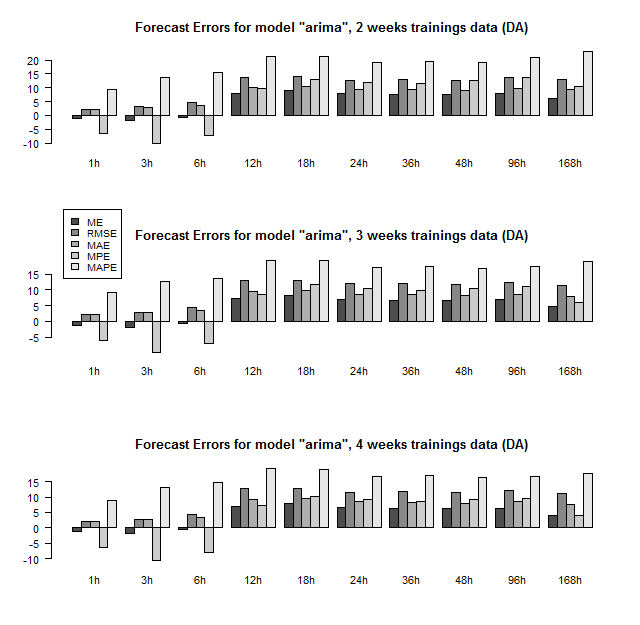
\includegraphics[width=0.85\textwidth]{figures/forecasting/da_sim_1_x_1w_1w_arima.png}
	\caption{Aggregated accuracy measures for ARIMA model and trainings data of 2, 3 and 4 weeks, Nord Pool Spot, Hamina}
	\label{fig:da_sim_1_x_1w_1w_arima}
\end{figure}

\begin{figure}[htbp]
	\centering
		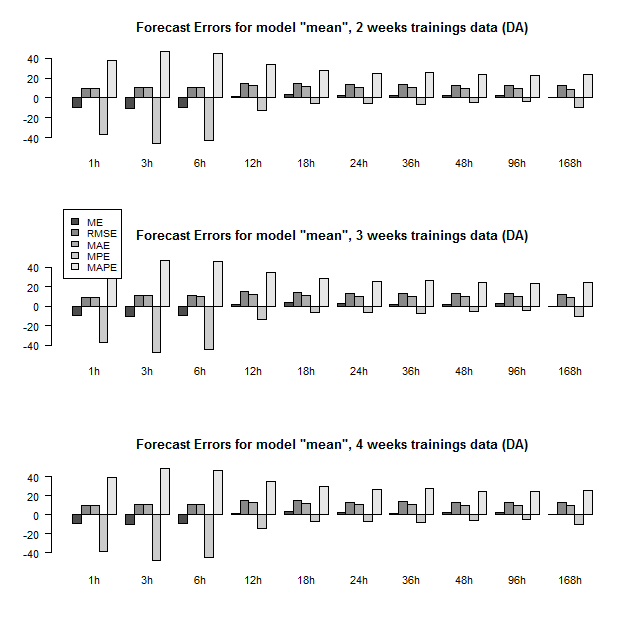
\includegraphics[width=0.85\textwidth]{figures/forecasting/da_sim_1_x_1w_1w_mean.png}
	\caption{Aggregated accuracy measures for Mean model and trainings data of 2, 3 and 4 weeks, Nord Pool Spot, Hamina}
	\label{fig:da_sim_1_x_1w_1w_mean}
\end{figure}


The result tables as well as graphs emphasize the observations made previously about model behavior. 

What can be observed by investigating the large scale forecast evaluation over all locations is that very different behaviors and scales of forecast errors exist for the same model over different locations (i.e.~datasets). An extreme example is the difference in forecast error distributions of the Nord Pool Spot and Belpex energy markets (tables \ref{ssec:app_tables_nord_pool_spot} and \ref{ssec:app_tables_belpex}, graphs \ref{ssec:app_graphs_nord_pool_spot} and \ref{ssec:app_graphs_belpex}). 

However, the seemingly extreme difference in forecast error distribution is mainly caused by exorbitant values of the MPE and MAPE error measures. This may be attributed to the occurrence of many low valued energy prices (close to zero) in the Belpex energy market which causes very high values for these methods. 

When comparing models TBATS, ARIMA followed by Mean and SES forecast models achieve the best results. Remarkably Mean forecasts outperform forecasts of SES models for almost all data sets of day ahead energy markets regarding forecast horizons $>= 12$. This behavior is reversed for real time markets where SES generally provides better performance. 

TBATS models exhibit the least forecast errors when they are able to capture seasonality appropriately. Otherwise these models show exponential growth of forecast errors over all measures. Due to this instability ARIMA models may be preferred as they exhibit stable forecast errors over most data sets and forecast horizons. 

Another note to error distribtions is that for the same forecast model similar patterns can be observed despite differences across energy markets. Concerning different trainings periods it can be observed that for most methods errors decrease with increasing trainings period, i.e.~four weeks of trainings data exhibits the least errors in most cases. 

Also different distributions are apparent for different error measures, e.g.~RMSE tend to increase with increasing forecast horizon whereas percentage errors (MPE and MAPE) tend to hit their lowest values for forecast horizons of 24h to 48h apart from horizons below 12h. 

Concerning the forecast error measures a focus has been laid on evaluating Root Mean Squared Errors (RMSE) since this measure has been proven to provide the most stable results. Percentage error measures such as Mean Percentage Error (MPE) and Mean Absolute Percentage Error (MAPE) tend to become numerically unstable for low values. Difference based measures such as Mean Error (ME) with non-absolute value differences provide little insights to the actual occurred forecast errors as positive and negative values might cancel each other out. 



\subsubsection{Aggregated Results}

Results have been aggregated over all forecast horizons and for each simulation which are shown in Tables \ref{tab:aggregated_results_nord_pool}, \ref{tab:aggregated_results_belpex}, \ref{tab:aggregated_results_isone} and \ref{tab:aggregated_results_pjm}. Best results have been formatted in bold in the tables. 

ARIMA and TBATS models showed superior results over all forecast horizons and training periods. TBATS models show best results when data can be modeled appropriately but exhibit anomalies in other cases. For different training periods a trend can be detected where forecast errors increase with increasing duration of the trainings period. However, ARIMA models show opposite results where forecast errors consistently decrease with increasing trainings period. 


% latex table generated in R 3.1.1 by xtable 1.8-2 package
% Fri Mar 25 19:35:50 2016
\begin{table}[ht]
\centering
\begin{tabular}{rrrrrrr}
  \hline
 & mean & ses & holts & holtwinters & arima & tbats \\ 
  \hline
2 weeks & 12.37 & 11.60 & 62.76 & 73.98 & 10.22 & \textbf{8.21} \\ 
  3 weeks & 12.57 & 11.60 & 62.90 & 75.55 & 9.50 & \textbf{8.57} \\ 
  4 weeks & 12.72 & 11.60 & 63.23 & 85.85 & 9.26 & \textbf{8.43} \\ 
   \hline
\end{tabular}
\caption{Results of evaluation for Hamina, Nord Pool Spot (DA)} 
\label{tab:aggregated_results_nord_pool}
\end{table}
% latex table generated in R 3.1.1 by xtable 1.8-2 package
% Fri Mar 25 19:35:50 2016
\begin{table}[ht]
\centering
\begin{tabular}{rrrrrrr}
  \hline
 & mean & ses & holts & holtwinters & arima & tbats \\ 
  \hline
2 weeks & 15.77 & 15.23 & 127.13 & 186.82 & \textbf{13.49} & 1.27E+50 \\ 
  3 weeks & 16.07 & 15.27 & 128.05 & 190.86 & 12.94 & \textbf{11.61} \\ 
  4 weeks & 16.25 & 15.30 & 127.03 & 186.37 & \textbf{12.87} & 2.49E+36 \\ 
   \hline
\end{tabular}
\caption{Results of evaluation for St.Ghislain, Belpex (DA)}
\label{tab:aggregated_results_belpex}
\end{table}
% latex table generated in R 3.1.1 by xtable 1.8-2 package
% Fri Mar 25 19:35:50 2016
\begin{table}[ht]
\centering
\begin{tabular}{rrrrrrr}
  \hline
 & mean & ses & holts & holtwinters & arima & tbats \\ 
  \hline
2 weeks & 26.42 & 23.61 & 235.84 & 417.39 & \textbf{24.11} & 5.45E+16 \\ 
  3 weeks & 26.36 & 23.56 & 238.92 & 686.95 & \textbf{22.26} & 1.64E+18 \\ 
  4 weeks & 26.84 & 23.32 & 268.10 & 437.85 & \textbf{21.83} & 2.18E+32 \\ 
   \hline
\end{tabular}
\caption{Results of evaluation for Portland, ISO-NE (RT)}
\label{tab:aggregated_results_isone}
\end{table}
% latex table generated in R 3.1.1 by xtable 1.8-2 package
% Fri Mar 25 19:35:50 2016
\begin{table}[ht]
\centering
\begin{tabular}{rrrrrrr}
  \hline
 & mean & ses & holts & holtwinters & arima & tbats \\ 
  \hline
2 weeks & 17.41 & 15.17 & 148.54 & 333.32 & \textbf{15.02} & 7.57E+13 \\ 
  3 weeks & 17.36 & 15.23 & 147.77 & 318.61 & 14.14 & \textbf{ 13.46} \\ 
  4 weeks & 17.34 & 15.29 & 148.67 & 357.82 & \textbf{14.11} & 5.44E+108 \\  
   \hline
\end{tabular}
\caption{Results of evaluation for Richmond, PJM (RT)}
\label{tab:aggregated_results_pjm}
\end{table}



\subsection{Conclusion of results}

From the discussion of the large scale forecast evaluation in the previous section various conclusions may be drawn. 

\paragraph{Model performance}

Concerning model performance ARIMA models showed the best results over different energy markets, trainings periods and forecast horizons. 
They showed consistently low forecast errors and appeared very stable throughout the simulations. Thus among the observed models ARIMA models may be the best choice considering forecast performance and statbility of results. 

\paragraph{Forecast Horizon}

Concerning forecast horizons it has been observed that horizons from 24 hours to 48 hours provide the best results when considering all models and trainings periods. 
For low horizons up to 12 hours different models may be suggested, i.e.~Holts model provide considerably lower forecast errors for forecast windows of 1 and 3 hours. 
For other than very short-term forecasts a forecast window of 24 to 48 hours provides best results. 

\paragraph{Training periods}

Different model training periods provide different results. Forecast errors have been observed to increase with the duration of the trainings period most of the time except for ARIMA models where the opposite behavior has been detected. Thus for ARIMA models a trainings period of 4 weeks is suggested for model generation. 

\paragraph{Forecast error measures}

As discussed before different forecast error methods provide different results for the same dataset. The ME provides an indication of the symmetry of the error distribution but little information about actual forecast performance. The MAE and RMSE provide a way of reliably model forecast errors where they achieve very similar results while the RMSE emphasizes outliers in the data. Percentage error measures have not been found to provide a reliable source of error measurements due to their instability for low values. Thus MAE and RMSE are considered the preferred way of modeling forecast errors. 








%%%%%%%%%%%%%%%%%%%%%%%%%%%%%%%%%%%%%%%%%
\chapter{Simulation Framework}
\label{ch:simulation_framework}
%%%%%%%%%%%%%%%%%%%%%%%%%%%%%%%%%%%%%%%%%





\section{Architecture of simulation framework} \label{sec:architecture_of_simulation_framework}


The simulation framework described in this section encompasses already described components in Section \ref{sec:r_java_simulation_framework} but enhances the framework by the cloud simulator. The cloud simulator should be able to assess the outcome of different scenarios encompassing data provided by the application server and utilizing forecast models generated on the application server in a previous step. 

The goal was to deliver a complete framework that can handle multiple data sources and is extendable for future work with possibly different data sets and an optional connection to a real cloud environment which could replace the simulated cloud environment that is connected to the framework in this implementation. 

The implementation consists of three parts which will be presented separately below. 

\paragraph{Data management} The first part represents the data handling and management interfaces presented in part already in Section \ref{sec:r_java_simulation_framework}. The purpose of this platform is to have a generic means of parsing and fetching data from various sources that can be defined in advance. For example, data may be fetched from local files that were previously retrieved from energy markets or remote web services that provide energy data of that respective energy market. In addition parsers for different file formats may be defined to automatically parse data and put it into the database for later retrieval. From there arbitrary queries may be executed to retrieve and aggregate data in a specific fashion and execute further tasks based on that data (e.g.~model generation). 

\paragraph{Forecast generation}
The second part consists of a collection of statistical methods that should assist in making accurate forecasts based on the previously collected data. A large scale evaluation of forecast methods has been presented in Section \ref{sec:forecast_model_evaluation} to determine the best forecast models for data from various energy markets. 
The purpose behind these statistical examinations is to provide meaningful and accurate forecasting models that can be utilized by the simulation framework. Eventually the performance of forecasts within the simulation should be examined and compared with approaches based solely on currently available data. It is expected that the application of accurate forecasts to energy price time series within the simulation improves overall performance and thus leads to a reduction in total energy costs. 

\paragraph{Cloud simulation}
The third part constitutes the actual cloud simulation which is based on a previously existing and sophisticated cloud simulator written in Python that incorporates cost models for energy and cooling expenses and is easily extendable by integrating custom schedulers \cite{lucanin2015philharmonic}. In this work custom settings have been applied to allow for a simulation that meets the needs of the framework to integrate different scenarios. Various parts of the simulator needed to be extended and a completely new scheduler has been built to schedule both cost aware and non-cost aware scenarios. It works together well with other parts of the framework s.t.~data can be retrieved from interfaces of the application server and integrated into the cloud simulation. The components are decoupled such that each of them may be replaced by other components easily provided that the same interface is used. 


\subsection{Architectural outline}

The architectural outline provides an overview of all components involved in the presented simulation framework and how they work together. All components may interact with one another via defined interfaces s.t.~either component may be replaced by a similar component with possibly different implementation details but same interfaces. 

\begin{figure}[htbp]
	\centering
	\vspace{-0.4in}
		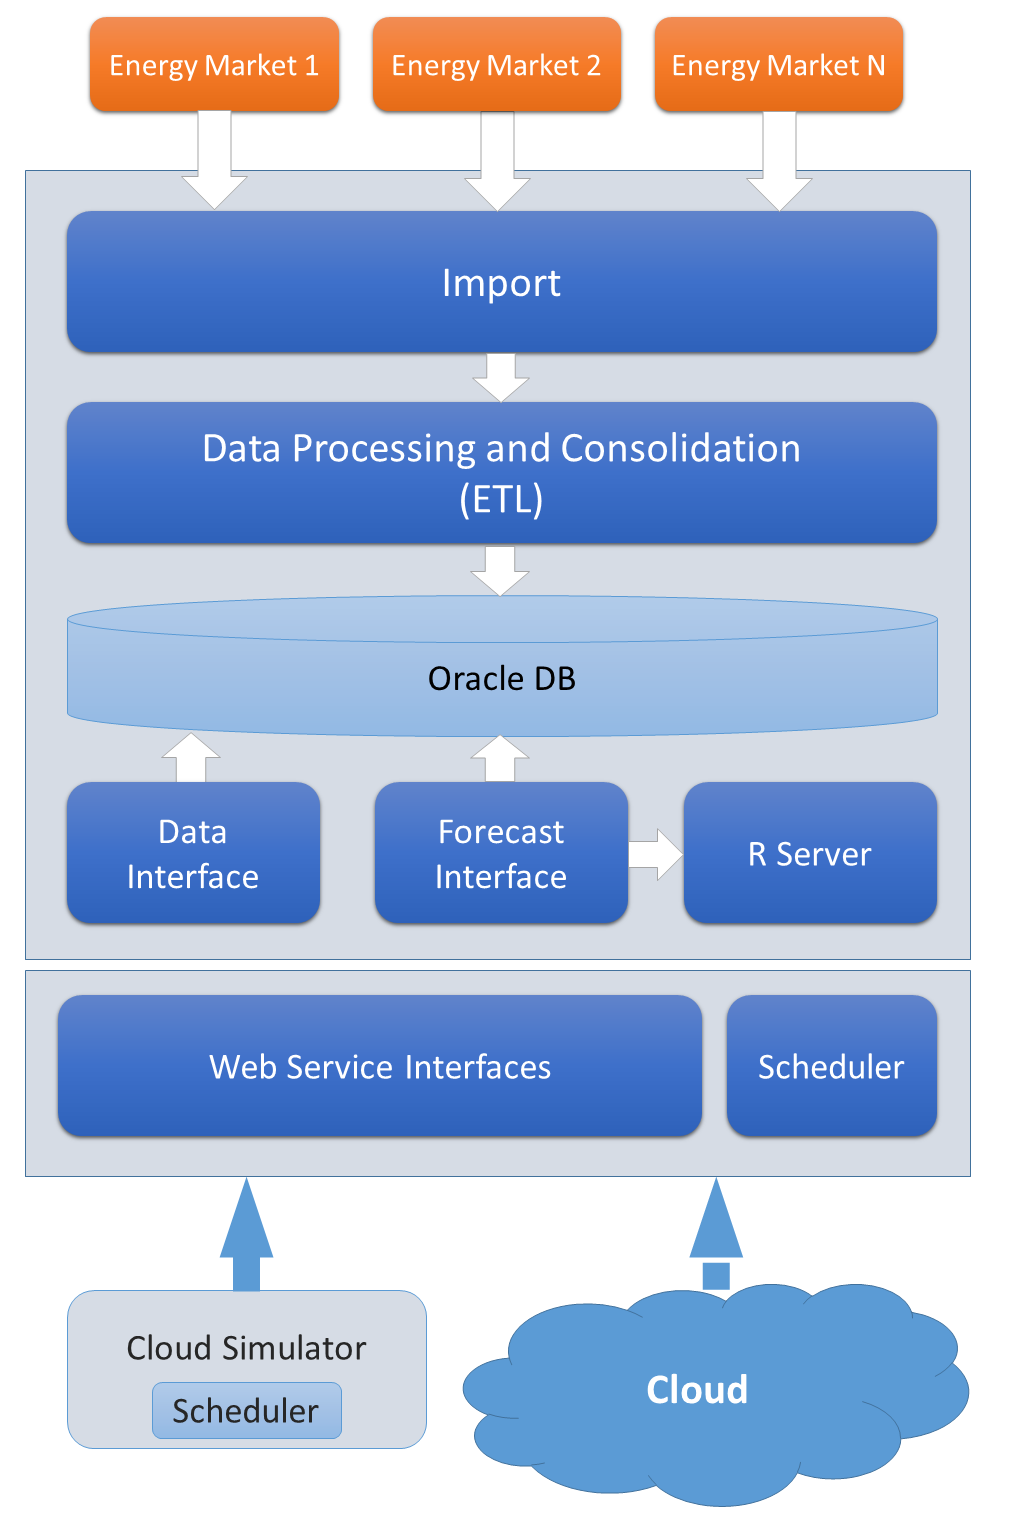
\includegraphics[width=0.5\textwidth]{figures/simulation_framework/Block_Diagram_Architecture.png}
	\caption{Architecture Block Diagram}
	\label{fig:Block_Diagram_Architecture}
\end{figure}

Figure \ref{fig:Block_Diagram_Architecture} depicts a block diagram of the simulation framework that shows which components are included and how they interact with one another. Data retrieval from the energy markets is done by the \textit{Import} module as the first action in the process. Several energy markets and their interfaces may be registered beforehand to retrieve data from these interfaces. 

From the \textit{Import} module the retrieved data is handed over to the \textit{Data Processing and Consolidation} module which transforms the data to a common format such that it can be fed to the database. This process is similar to the well known ETL process (Extract Transform Load)\cite{vassiliadis2002conceptual} which extracts data from various sources, transforms it into a defined data format and loads it into a data warehouse or database. The applied process in this work is similar as parsers for different file formats may be defined that can be configured to parse data from different sources. After the data transformation process the retrieved energy prices are stored in the database from where they may be retrieved for simulation purposes. 

The \textit{Data Interface} contains all methods for data retrieval of prices stored in the database. Thus data is provided to web service interfaces for arbitrary time periods and both day ahead and real time prices. In addition it is possible to query for local or DST corrected bidding dates or retrieving data adjusted to a predefined currency (e.g.~dollars). 

The \textit{Forecast Interface} handles all requests related to model generation and forecasting which is provided by the \textit{R server}. It contains methods defined for large scale forecast evaluation, automated model generation and calculating forecasts for generated models. 

The \textit{R server} does not directly connect to the database but retrieves energy data from the \textit{Forecast Interface} which triggers the generation of forecasting models. The interface used to communicate from Java to R (and vice versa) is called \textit{rJava} \cite{rforge2007rjava} which provides a wrapper to directly execute R code in Java. 

The \textit{Scheduler} may be configured to trigger data import from specific energy markets at a defined time interval (e.g.~every hour or once per day). In this process it may also trigger the generation of forecasting models as the model generation process can take a considerable amount of time depending on the amount of training data provided to the model.

Finally the \textit{Web Service Interfaces} are a means of providing data to external components such as the simulator or a real cloud. 
These interfaces provide data retrieval and forecast interfaces as described previously. They can be used to get historical data from different energy markets and locations as well as time periods for the purpose of getting customized data for simulations. In addition they provide a convenient way of retrieving forecast data for specific locations and periods of time. As soon as forecasting models have been generated for a specific period of time forecasts can be provided instantly for that period. 



\subsection{Components and Interfaces}

In this section a more detailed view on the various components of the framework is provided and the interfaces that exist between them. Figure \ref{fig:Component_Diagram} shows this view in form of a component diagram. 

\begin{figure}[htbp]
	% used to position the image at the horizontal center of the page
	\hspace*{-0.8in}
		% include the graphic rotated by a 90 degree angle and scale to paperwidth and height
		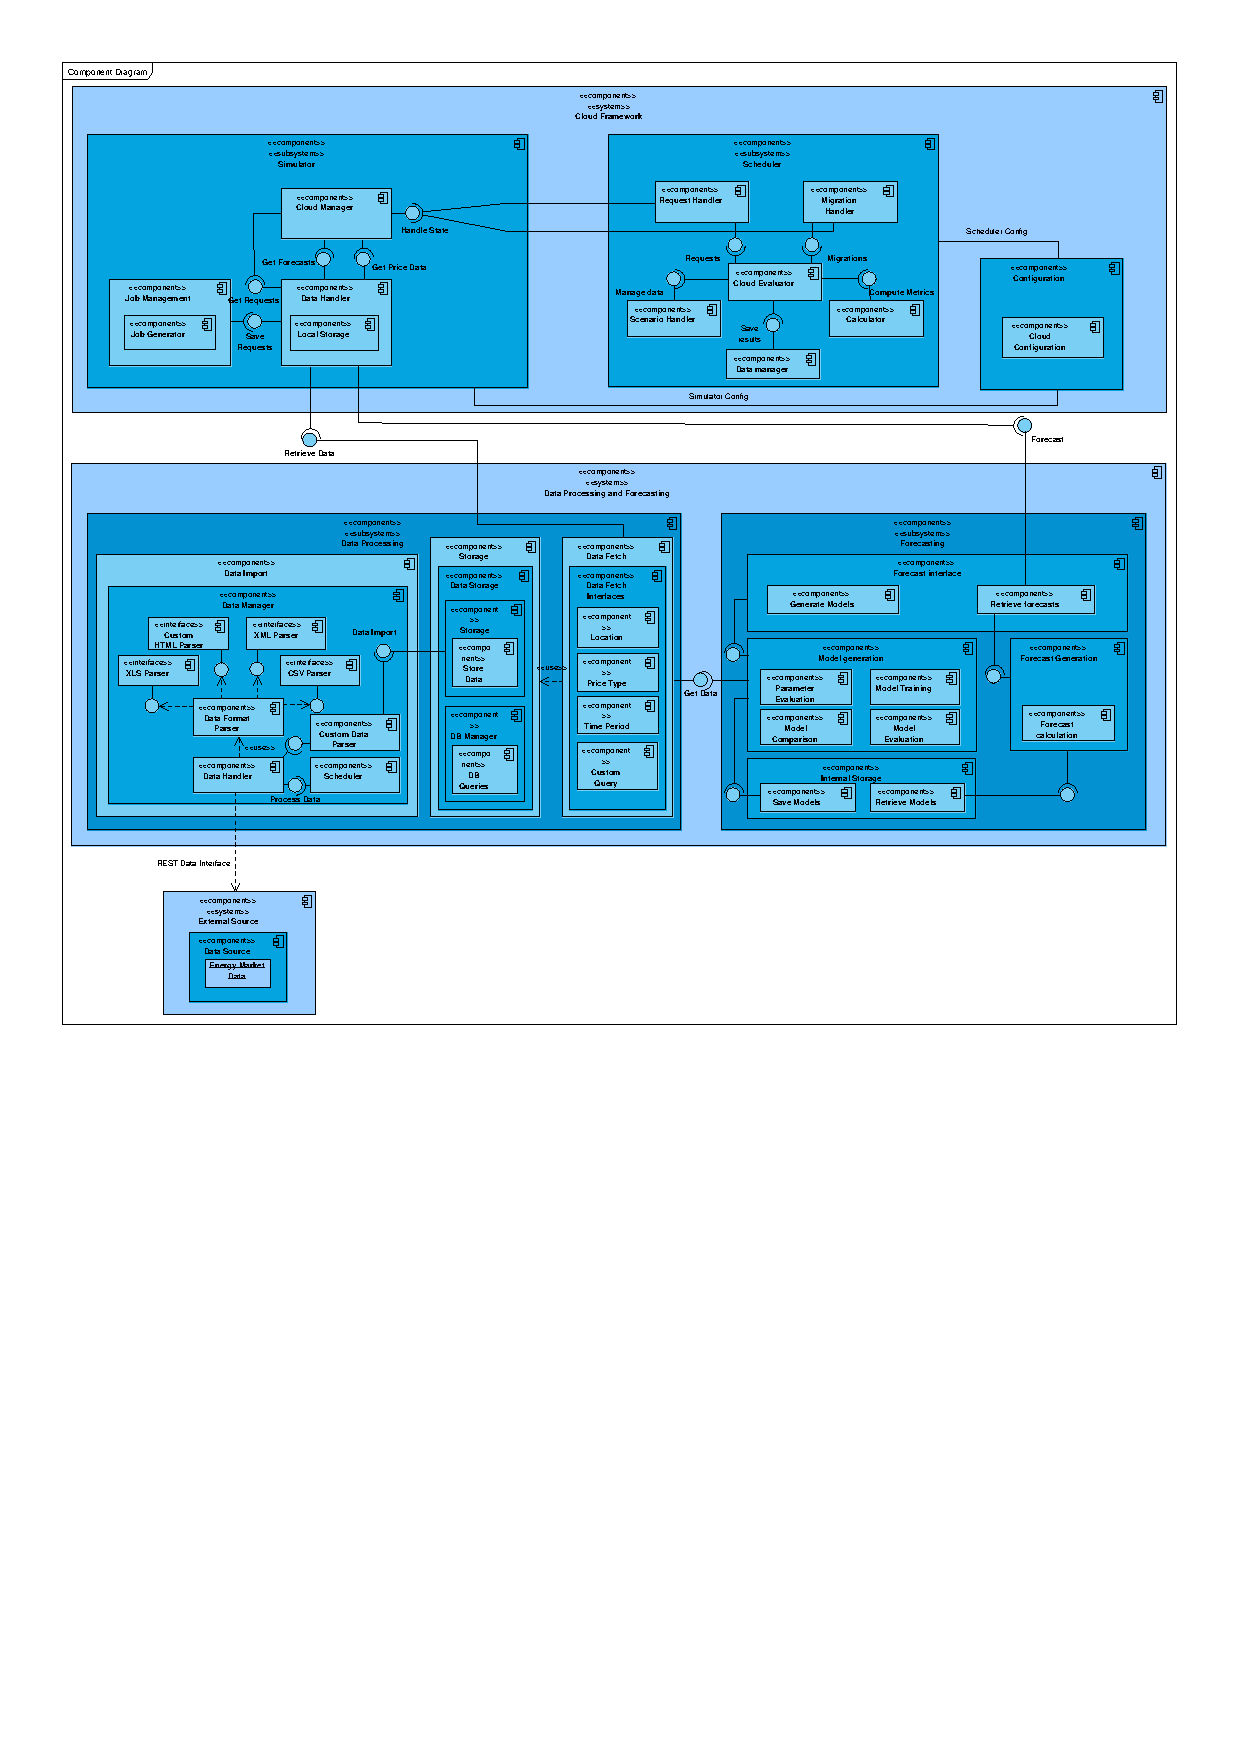
\includegraphics[angle=90,width=\paperheight,height=\paperwidth,keepaspectratio=true]{figures/simulation_framework/Component_Diagram.pdf}
	\caption{Component Diagram}
	\label{fig:Component_Diagram}
\end{figure}

The diagram basically consists of two parts, the \textit{Cloud Framework} and \textit{Data Processing and Forecasting} components. The Cloud Framework contains the \textit{Simulator} and \textit{Scheduler} and is implemented in python \cite{lucanin2015philharmonic}. It is responsible for the actual simulation and application of scheduling algorithms. The Data Processing and Forecasting part consists of the \textit{Data Processing} and \textit{Forecasting} components and is implemented on the Java application server. This component is responsible for data management and forecast operations.

\textit{Data Processing} consists of \textit{Data Import}, \textit{Storage} and \textit{Data Fetch} components. 

The \textit{Data Import} component is responsible to retrieve data from previously registered energy markets as indicated by the dashed line connection to the external data source. The data import can as well be triggered by the scheduler which calls the respective services at the Data Handler. The Data Handler uses appropriate parsers to extract data into a common processable format. When the processing of data is finished the 
data is fed to a \textit{Custom Data Parser} which handles peculiarities such as DST time changes and missing energy price data. The cleared data is then handed on to the Storage component which saves the data to the database. 

The \textit{DB Manager} in the Storage component provides methods for data retrieval which is used by the \textit{Data Fetch} component. 
Different interfaces are provided for executing queries of stored energy price data, e.g.~by location, price type or custom queries. This can in turn be used by the simulator to retrieve energy price data. 

The \textit{Forecasting} component provides interfaces to \textit{Generate Models} and \textit{Retrieve Forecasts}. 

The \textit{Generate Models} component refers to the \textit{Model Generation} component with \textit{Parameter Evaluation}, \textit{Model Training}, \textit{Model Evaluation} and \textit{Model Comparison}. Before model generation it refers to the Data Fetch component for retrieval of energy price data of the desired time period. After the model(s) have been generated they are saved to the \textit{Internal Storage}, i.e.~in the file system of the application server. 

For retrieving forecasts the \textit{Retrieve Forecasts} interface is queried which in turn calls the \textit{Forecast Generation} component. Thus forecasts may be retrieved from models which have been generated and stored previously within the Internal Storage component. 

fetches data from the database and does some data preprocessing that is used for forecasting. After the data has been processed and formatted appropriately it is ready to be analyzed by statistical methods to determine which forecasting model suits best for the selected time series. Different models are trained and compared and the best model is chosen. It is then selected by the Forecast Module and the actual forecasts are calculated which can be queried via a provided public interface that is exposed to external systems. 

The \textit{Cloud Framework} uses the historical price data provided by the \textit{Data Fetch} component to run simulations for various scenarios. It is read into a local storage by a \textit{Data Handler} for further processing of the price data in simulations. In addition, forecasts may be retrieved by the Data Handler at this stage to prevent having an open connection to the application server during simulations. Job requests are generated by the \textit{Job Management} component which reflect certain characteristics or requirements of tasks that should be processed by the Cloud Framework. Requests and energy prices are read by the \textit{Cloud Manager} that keeps track of the cloud's current state. The state is retrieved and modified by the scheduler which retrieves data from \textit{Request} and \textit{Migration Handlers} which is then fed to the \textit{Cloud Evaluator}. The evaluator decides on needs for migrations depending on the given scenario defined by the \textit{Scenario Handler}. It uses a \textit{Calculator} component to compute metrics such as migration energy and VM downtime. 

At each step the Cloud Evaluator gets current request and migration demands and checks metrics for VM migration. If it retrieves a positive result the resources are moved to the respective server. Results are handled by a Data Manager component after the simulation finishes. Both scheduler and simulator components are configurable by a config file defined by the \textit{Cloud Configuration} component. Thus new configuration options are easily added and can be changed at any time to adjust the output of simulations. 




\section{Modeling migration energy} \label{sec:modeling_migration_energy}

Besides the structural outline presented in the previous section important methodologies used by the cloud simulator and scheduler are investigated in detail in the following sections. 

Since the goal of the simulation presented in this work is to reduce energy costs by intelligently migrating resources across geo-distributed data centers an important metric to consider is the migration energy and migration costs. An outstanding paper on this topic has been presented in \cite{liu2013performance} where the energy and downtime related to a VM migration are examined and formalized in detail. This paper has been briefly outlined in Section \ref{ssec:performance_and_energy_modeling_of_virtual_machines}. 

The impact of the \textit{writable working set} (WWS) of an application on VM migration time and total downtime is described in \cite{clark2005live} (see also Section \ref{ssec:live_migration_of_virtual_machines}). It is the set of most frequently updated memory pages in a running application which is dirtied in each pre-copy round of an VM migration \cite{clark2005live, liu2013performance}. Thus a large WWS can increase migration downtime significantly with a high amount of pages dirtied in each pre-copy iteration (dirty page rate) that ultimately have to be sent at a time at the final stop-and-copy phase. 

With increasing number of iterations more data has to be transferred and transmission costs rise. The final stop-and-copy phase is reached when any of the following conditions has been met (as implemented in this work): 

\begin{enumerate}[label=\textnormal{(\arabic*)}]
	\item memory dirtying rate exceeds memory transmission rate \label{itm:condition1}
	\item the remaining dirty memory falls below a predefined threshold \label{itm:condition2}
	\item the number of pre-copying iterations exceeds a defined maximum \label{itm:condition3}
\end{enumerate}

From \cite{liu2013performance} the proposed base model for VM migration has been implemented. It is based on a list of parameters defined in Table \ref{tab:migration_parameters}. 

Migration energy, load and downtime metrics have been implemented based on the following equations: 

\begin{align}
	\lambda &= \frac{D}{R} \label{eq:m_lambda} \\
	V_i &= D \frac{V_{mem}}{R} \lambda^{i-1} = V_{mem} \lambda^i \label{eq:m_v_i} \\
	T_i &= \frac{D T_{i-1}}{R} = \frac{V_{mem} D^i}{R^{i+1}} = \frac{V_{mem} \lambda^i}{R} \label{eq:m_t_i} \\
	V_{mig} &= \sum_{i=0}^n V_i = V_{mem} \frac{1 - \lambda^{n+1}}{1 - \lambda} \label{eq:m_v_mig} \\
	T_{mig} &= \sum_{i=0}^n T_i = \frac{V_{mem}}{R} \frac{1 - \lambda^{n+1}}{1 - \lambda} \label{eq:m_t_mig} \\
	n &= \left\lceil \log_{\lambda} \frac{V_{thd}}{V_{mem}} \right\rceil \label{eq:m_n} \\
	T_{down} &= T_n + T_{resume} \label{eq:m_t_down} \\
	E_{mig} &= E_{sour} + E_{dest} \label{eq:m_e_mig} \\
	&= (\alpha_s + \alpha_d) V_{mig} + (\beta_s + \beta_d) \nonumber \\
	&= \alpha V_{mig} + \beta = 0.512 V_{mig} + 20.165 J \nonumber \\
	V_n \le V_{thd} &\Leftrightarrow V_{mem} \lambda^n \le V_{thd} \label{eq:m_v_n}
\end{align}


\begin{table}[htbp]
\centering
\begin{tabular}{ll}
  \hline
	Parameter & Description \\ 
  \hline
		$V_{mem}$ & The total size of the VM memory \\ 
		$V_{mig}$ & The total migration load (network traffic) during migration \\ 
		$T_{mig}$ & Total migration time \\ 
		$V_i$ & Migration load for the i-th iteration \\ 
		$T_i$ & Migration transfer time for the i-th iteration \\ 
		$T_{down}$ & Effective downtime of migration \\ 
		$T_{resume}$ & Time to resume operation of VM on other host \\ 
		$E_{mig}$ & Total migration energy \\ 
		$\alpha, \beta$ & Model parameters for migration energy \\
		$R$ & Memory transmission rate or bandwidth \\ 
		$D$ & Dirty page rate of application \\ 
		$V_{thd}$ & Threshold of remaining memory to end pre-copy phase \\ 
		$\lambda$ & Convergence coefficient of VM migration \\ 
		$n$ & The index of the last pre-copy iteration \\
		$n_{max}$ & The maximum number of pre-copy iterations \\
   \hline
\end{tabular}
\caption{Parameters used in the migration algorithm}
\label{tab:migration_parameters}
\end{table}


Equation \ref{eq:m_lambda} defines $\lambda$ as the convergence coefficient of the migration since it states how fast the migration converges to the final stop-and-copy phase. 

$V_i$ and $T_i$ in Equations \ref{eq:m_v_i} and \ref{eq:m_t_i} denote the migration load and time in pre-copy iteration $i$ whereby these metrics depend greatly on the convergence coefficient $\lambda$. If $D < R$ then $\lambda < 1$ and migration load will eventually fall below the defined threshold $V_{thd}$ (assuming a writable working set less than $V_{thd}$). 

$V_{mig}$ and $T_{mig}$ in Equations \ref{eq:m_v_mig} and \ref{eq:m_t_mig} describe the total migration load and time which is defined as the sum of migration load and time for all iterations $i$ up to the last pre-copy iteration $n$. Equation \ref{eq:m_n} defines the index of the last iteration after which the stop-and-copy phase is executed. 

Equation \ref{eq:m_t_down} describes the effective downtime of the migration consisting of the time needed for the last iteration (stop-and-copy phase) and the time needed to resume operation of the newly created VM. Equation \ref{eq:m_e_mig} formalizes migration energy as the sum of source and destination energy ($E_{sour}$ and $E_{dest}$). Model parameters $\alpha$ and $\beta$ can each be defined separately for source and destination (e.g.~$\alpha_s$ and $\alpha_d$). However homogenous parameters have been assumed and estimated as described in \cite{liu2013performance} for both source and destination (last line of Equation \ref{eq:m_e_mig}). 

The condition for reaching the defined memory threshold is depicted in Equation \ref{eq:m_v_n}. As defined before $n$ is the index of the last pre-copy iteration where remaining memory should be below threshold $V_{thd}$ (see definition of condition \ref{itm:condition2}). In case this condition is not met and $n = n_{max}$ the pre-copy phase is aborted and all remaining memory is transferred to the destination host (condition \ref{itm:condition3}). When condition \ref{itm:condition1} is detected the stop-and-copy phase is executed immediately. 




\section{SLA management} \label{sec:sla_managemenet}

In this work the Service Level Agreement (SLA) is specified as the guaranteed availability of VMs. Cloud providers such as Google or Amazon provide SLAs for different levels of guaranteed availability \cite{google2015compute, amazon2013sla}. In this work the 99.95\% availability contract as depicted on the Google Compute Cloud \cite{google2015compute} has been chosen as a standard metric valid for all VMs in simulations. The cloud provider establishes this contract in accordance with the customer which states that a running VM will have an uptime duration of at least 99.95\% of the total runtime of the VM. If the total runtime exceeds one month (which is the billing period) the percentage of uptime duration is related to this period only. Thus the total downtime of a VM over the applicable time period is not allowed to exceed 0.05\% of that time period (e.g.~the maximum allowed downtime per hour would be $3600s * 0.0005 = 1.8s$). 

In case this criterion can not be met the cloud provider is obliged to pay penalties, depending on the total downtime. The amount of penalties and the relation to the total downtime is depicted in Table \ref{tab:sla_penalties}. 


\begin{table}[htbp]
\centering
\begin{tabular}{ll}
  \hline
	Uptime Percentage & Percentage of penalty relative to a user's total cost	 \\
  \hline
	99.00\% - < 99.95\%	& 10\% \\
	95.00\% - < 99.00\%	& 25\% \\
	< 95.00\%				& 50\% \\
   \hline
\end{tabular}
\caption{VM downtime vs SLA penalties}
\label{tab:sla_penalties}
\end{table}


For a VM having an uptime of below 99.95\% but above 99\% the user has to be paid a penalty of 10\% of the total amount the user would have originally paid. Analogously if uptime falls below 99\% but above 95\% the user is paid back 25\% and for uptimes below 95\% of the time the user is refunded 50\% of the price. 

Different SLA availability contracts are available, i.e.~Google storage provide only a reduced availability of 99.9\% or even 99\% \cite{google2015storage}. However these have not been considered in this work. 

\section{Cost optimization based on utility function}

\subsection{Utility function definition}

Problems comprising multiple criteria with different associated weights have been researched in different contexts \cite{angilella2004assessing, dulmin2003supplier}. These kind of problems are commonly referred to as \textit{Multiple Criteria Decision Aid} (MCDA) where for different possibly contradicting criteria the best solution should be determined considering custom criteria weights \cite{dulmin2003supplier}. 

Utility functions have been proposed as a way of solving multi criteria decision problems \cite{angilella2004assessing, afriat1967construction}. 
For such problems a so called \textit{Decision Maker} (DM) manages a set of choices or alternatives $A = \{a,b,c,\ldots\}$ and a fixed set of $n$ criteria $G = \{g_1,g_2,\ldots,g_i,\ldots,g_n\}$, where $g_i : A \rightarrow \mathfrak{R}$. 
In \cite{angilella2004assessing} a \textit{marginal weak preference relation} is further defined as $\succsim_i, i = 1,\ldots,n$ on the set of alternatives $A$ such that $\forall a,b \in A, a \succsim_i b$. The meaning of the relation is ``$a$ is at least as good as $b$ regarding criterion $g_i$''. 
Thus for each $g_i \in G$ and $\forall a,b \in A$ it holds that $g_i(a) \geq g_i(b) \Leftrightarrow a \succsim_i b$. 

A comprehensive weak preference relation $a \succsim b$ is defined as $\forall a,b \in A, a \succsim b$ and means ``$a$ is globally at least as good as
$b$''. 
A utility model may be defined from that relation in case it is a complete preorder \cite{angilella2004assessing}:

\begin{align}
	\forall a,b \in A: U(g(a)) \geq U(g(b)) \Leftrightarrow a \succsim b \label{eq:comprehensive_weak_preference_relation}
\end{align}	

with $U : \mathfrak{R}^n \rightarrow \mathfrak{R}$ and $U(g(.)) = U(g_1,g_2,\ldots,g_i,\ldots,g_n)$ \\
As stated in \cite{angilella2004assessing} an additive utility function may be derived from the relation in Equation \ref{eq:comprehensive_weak_preference_relation}:

\begin{equation}
	U(x) = \lambda_1 u_1 (g_1(x)) + \lambda_2 u_2 (g_2(x)) + \ldots + \lambda_n u_n (g_n(x)), x \in A
\label{eq:definion_of_additive_utility_function}
\end{equation}

with $\lambda_1,\lambda_2,\ldots,\lambda_n \in \mathfrak{R}^+$ and $u_i$ defined as non-decreasing marginal utility functions. \\
\\
Based on the utility function definition in Equation \ref{eq:definion_of_additive_utility_function} a utility function has been introduced to the Cloud Scheduler with $\lambda_1,\lambda_2,\ldots,\lambda_n \in [0,1]$ denoting the \textit{weights} and $u_i$ denoting functions that normalize criteria values $g_i$ such that $g_1,g_2,\ldots,g_i,\ldots,g_n \in [0,1]$. 




\subsection{Cloud Scheduler and utility function}

The goal of the Cloud Scheduler is to optimize resource scheduling with respect to current and future energy prices. In order to take into account different criteria and choose VMs exhibiting the best fit for migration a utility function has been implemented that evaluates the current cloud state and provides aid in finding VMs with best conditions for migration. 

The utility function definition is outlined in Equation \ref{eq:cloud_scheduler_utility_function}. 

\begin{equation}
	U(v) = \sum_{i=1}^k w_i c_i (v)
\label{eq:cloud_scheduler_utility_function}
\end{equation}

where $w_i$ denote the weights and $c_i$ denote the normalized criteria values which are $\lambda_i$ and $u_i(g_i(x))$ in Equation \ref{eq:definion_of_additive_utility_function}, respectively. Criteria values (and thus the utility function as well) are defined s.t.~a value of 0 denotes the worst result whereas a value of 1 is considered the best result, i.e.~VMs associated with an utility value near 1 are very likely to be migrated. 

In Table \ref{tab:list_of_utility_criteria} all criteria that have been defined in the Cloud Scheduler are displayed. 

\begin{table}[htbp]
\centering
\begin{tabular}{lll}
  \hline
	Criteria & Name	& Description \\
  \hline
	$c_1$ & probability of SLA penalty & probability that an SLA penalty will occur after migration \\
																	  && (based on experienced downtime) \\
	$c_2$ & estimated migration energy & the expected migration energy depending on VM memory, \\
																		&& bandwidth and dirty page rate \\
	$c_3$ & remaining VM duration & number of unit time spans the job or VM is still running \\
	$c_4$ & data center load & load of DC where VM is located, balance load across DCs \\
	$c_5$ & estimated cost benefit & expected migration benefit (cost savings) given the \\
																		&& current conditions \\
   \hline
\end{tabular}
\caption{List of utility criteria}
\label{tab:list_of_utility_criteria}
\end{table}

Each of the criteria above describes one metric by which a virtual machine running within the cloud simulation can be evaluated such that values for different VMs may be compared and VMs having a utility value greater than a defined threshold may then be considered for migration. Thus a utility threshold $U_{thd}$ is defined s.t.~VMs are scheduled for migration if $U(v) \geq U_{thd}$. 

\subsubsection{Criteria definition}

In the following, each criterion is formalized and described in detail. 

\paragraph{Probability of SLA penalty}

As outlined in Section \ref{sec:sla_managemenet} it is vital for cloud providers to ensure that VM downtimes only occur rarely during their execution. 
Thus the \textit{probability of an SLA penalty} is an important metric to consider when performing migrations as they may lead to extensive downtimes. 

All parameters used in the following equations are outlined in Table \ref{tab:sla_penalty_parameters}. 

\begin{table}[htbp]
\centering
\begin{tabular}{ll}
  \hline
	Parameter & Description	 \\
  \hline
	$v_{dur}$ & Total expected duration of VM $v$	 \\
	$v_{SLA}$ & SLA availability percentage agreed for VM $v$	 \\
	$v_{SLA_{TH}}$ & Threshold for SLA violation for VM $v$	 \\
	$loc$ & set of locations included in the simulation	 \\
	$down_{acc}(v,t)$ & accumulated downtime for VM $v$ \\
	$cond_{pred}(v,l,t)$ & condition for prediction of down time of VM $v$ \\
	$dt_{v}(t)$ & function to determine if a down time occurred for VM $v$ at time $t$	 \\
	$p_{SLA}(v,l,t)$ & probability of SLA penalty for VM $v$ when migrated to location $l$ at time $t$	 \\
	$pen_{SLA}(v,l,t)$ & adjusted probability of SLA penalty when migrating VM $v$ to location $l$ at time $t$	 \\
	$best_{SLA}(v,t)$ & minimum probability of SLA penalties when considering all locations \\
   \hline
\end{tabular}
\caption{Parameters used in equations}
\label{tab:sla_penalty_parameters}
\end{table}

The corresponding equations are outlined below. 

\begin{align}
	dt_v(t) &= \left\{
								\begin{array}{@{}ll@{}}
									1, & \text{if VM } v \text{ was down at time } t \\
									0, & \text{otherwise}
								\end{array}\right. \label{eq:sla_dt_v}\\
	down_{acc} (v,t) &= \sum_{z=0}^t dt_v(z) \label{eq:sla_down_acc}\\
	v_{SLA_{TH}} &= v_{dur} \left( 1 - \frac{v_{SLA}}{100} \right) \label{eq:sla_v_sla_th} \\
	p_{SLA} (v,l,t) &= \frac{down_{acc}(v,t) + T_{down}(v,t)}{v_{SLA_{TH}}} \label{eq:sla_p_sla}\\
	cond_{pred} (v,l,t) &= down_{acc}(v,t) + T_{down}(v,t) - v_{SLA_{TH}} \label{eq:sla_cond_pred}\\
	pen_{SLA} (v,l,t) &= \left\{
													\begin{array}{@{}ll@{}}
														1, & \text{if}\ cond_{pred} (v,l,t) > 0 \\
														p_{SLA} (v,l,t), & \text{otherwise}
													\end{array}\right. \label{eq:sla_pen_sla}\\
	best_{SLA} (v,t) &= \min_{l \in loc, l \neq v_{loc}} pen_{SLA} (v,l,t) \label{eq:sla_best_sla}\\
	c_1(v,t) &= 1 - best_{SLA} (v,t)  \label{eq:sla_c_1}
\end{align}

Equations \ref{eq:sla_dt_v} and \ref{eq:sla_down_acc} show formulas of aggregated downtime of VM $v$ up to time $t$. 
$v_{SLA_{TH}}$ is the threshold in time periods that describes up to which downtime duration can be tolerated considering the SLA assigned to this VM ($v_{SLA}$). 

A simple probability measure for experiencing an SLA penalty is shown in Equation \ref{eq:sla_p_sla} where the sum of accumulated downtimes $down_{acc}$ and the predicted downtime $T_{down}$ is set in relation to the SLA threshold. If $p_{SLA} \geq 1$ an SLA penalty will occur considering the predicted downtime. 
The corresponding conditional equation to test expected downtime against SLA threshold is depicted in Equation \ref{eq:sla_cond_pred}. 

$pen_{SLA}$ restricts the outcome of the SLA probability $p_{SLA}$ to the range $[0,1]$. It denotes the probability of SLA penalty when migrating VM $v$ to location $l$ at time $t$ (Equation \ref{eq:sla_pen_sla}). The $best_{SLA}$ metric in Equation \ref{eq:sla_best_sla} calculates the min of $pen_{SLA}$ for all locations except the one where VM $v$ is located to evaluate the best (lowest) probability of SLA penalty at the current point in time. 

Finally the criterion $c_1$ is described by inverting the value of $best_{SLA}$ regarding the range $[0,1]$ (Equation \ref{eq:sla_c_1}). The purpose of that is to provide values closer to one for ``good'' utility values and values close to zero for ``bad'' utility values. 


\paragraph{Estimated migration energy}

The \textit{estimated migration energy} for live migration of virtual machines is closely related to the total migration load that is transferred during the process \cite{liu2013performance}. The results are depending greatly on the amount of VM memory to transfer, bandwidth between source and destination hosts and dirty page rate of the application to be transferred. 

This metric uses the formula for migration energy already defined in Section \ref{sec:modeling_migration_energy}. 
The corresponding equations for this metric are outlined below. 

\begin{align}
	E_{rel} (v,l) &= \frac{E_{mig}(v,l)}{\max_{v_{mig} \in VM, v_{mig_{loc}} \neq l} (E_{mig}(v_{mig},l))} \label{eq:mig_e_rel} \\
	E_{best} (v,t) &= \min_{l \in loc, l \neq v_{loc}} E_{rel} (v,l) \label{eq:mig_e_best}\\
	c_2(v,t) &= 1 - E_{best}(v,t) \label{eq:mig_c_2}
\end{align}


where $VM$ denotes the set of VMs active in the simulation. \\
The metric $E_{rel}$ (Equation \ref{eq:mig_e_rel}) computes the relative migration energy where the calculated energy for the current VM is related to the maximum of expected migration energy of all VMs when migrated to location $l$. 

$E_{best}$ denotes the minimum relative migration energy when considering migration to all locations (Equation \ref{eq:mig_e_best}). 

$c_2$ is then the additive inverse of $E_{best}$ within the interval $[0,1]$ (Equation \ref{eq:mig_c_2}). 



\paragraph{Remaining VM duration} \label{par:remaining_vm_duration}

The \textit{remaining VM duration} is a simple metric to have the possibility to favor those VMs that are running for a longer period of time, e.g.~to mitigate SLA penalties. 

It is defined as follows: 

\begin{align}
	remaining(v,t) &= \frac{v_{rem}(t)}{\max_{vm \in VM} vm_{rem}(t)} \label{eq:remaining_dur} \\
	c_3 (v,t) &= remaining(v,t) \label{eq:remaining_dur_result}
\end{align}

where $v_{rem}$ denotes the remaining duration for VM $v$ at time $t$. 

Equation \ref{eq:remaining_dur} is a relative measure of a VM's remaining duration in relation to the maximum of remaining durations of currently running VMs. The result criterion $c_3$ in Equation \ref{eq:remaining_dur_result} is just assigned the metric itself as longer running VMs should be favored. 


\paragraph{Data center load}

The \textit{data center load} is a global metric to achieve better load balancing across data centers, i.e.~VMs are favored for migration from data center locations exhibiting very high load. 

\begin{align}
	load(v,t) &= \frac{load_{DC_v}}{\max_{vm \in VM} load_{DC_{vm}}} \label{eq:load}\\
	c_4 (v,t) &= load(v,t) \label{eq:load_result}
\end{align}

where ${load_{DC_v}}$ is the current load at the data center where VM $v$ is currently located. 

The relative load of the data center where VM $v$ is currently located in relation to the maximum load is depicted in Equation \ref{eq:load}. The result criterion $c_4$ in Equation \ref{eq:load_result} is again assigned the previous metric directly as VMs located at data centers exhibiting high load are favored for VM migrations. 



\paragraph{Estimated cost benefit}

The \textit{estimated cost benefit} can probably be regarded as the most important criterion above all introduced criteria as it allows to optimize VM migrations with respect to resulting costs. 

This metric takes into account future energy prices in case forecasts are enabled within the simulation. Thus the estimated cost benefit is not only calculated based on current energy prices but calculates the mean for each forecast horizon and location and returns the maximum evaluated difference of prices between two locations and forecast horizons. 

Equations are listed below. 

\begin{align}
	fce(i,j,r) &= \sum_{h=0}^r fc_i(h) - fc_j(h) \label{eq:es_fce}\\
	max_{fc}(v,t) &= \left\{
								\begin{array}{@{}ll@{}}
									\min (v_{rem}(t),fc_{max}), & \text{if } fc_{en} \text{ is true } \\
									0, & \text{otherwise}
								\end{array}\right. \label{eq:es_max_fc}\\
	es(v,t) &= \max_{i \in loc, i \neq v_{loc}} fce(v_{loc},i,max_{fc}(v,t)) \label{eq:es_es} \\
	cb(v,t) &= \frac{es(v,t)}{\max_{v_{mig} \in VM}  es(v_{mig},t)} \label{eq:es_cb} \\
	c_5(v,t) &= cb(v,t) \label{eq:es_c_5}
\end{align}

where $fc_{max}$ is the maximum forecast horizon taken into account, $v_{rem}$ is the remaining duration for VM $v$ (see paragraph in \ref{par:remaining_vm_duration}) and $fc_{en}$ is a logical variable indicating whether forecasts are enabled or not. 

The mean difference (forecast estimation) between each two locations summed up over all forecast horizons up to a defined maximum is given in Equation \ref{eq:es_fce}. For two given locations $i$ and $j$ the mean difference is calculated up to a maximum of $r$ forecast horizons. 

In Equation \ref{eq:es_max_fc} the maximum applicable forecast horizon is determined which is based on the remaining VM duration but can not exceed $fc_{max}$. The remaining duration is taken into account as beneficial price differences can only be taken advantage of as long as the VM is still active. 

Equation \ref{eq:es_es} denotes the maximum estimated cost benefit when migrating VM $v$ at time $t$. It determines the maximum value across all forecast estimations $fce$ for the given VM. 
The resulting cost benefit is defined in Equation \ref{eq:es_cb} where the estimated cost benefit of VM $v$ is set in relation to the maximum cost benefit of all VMs. 

The criterion for the estimated cost benefit is set to the resulting cost benefit since VMs with the highest expected cost benefit should be more likely to be migrated (Equation \ref{eq:es_c_5}). 


\subsubsection{Discussion}

The presented metrics have been chosen to get a diverse set of criteria where different criteria may be emphasized. Some of the criteria are opposite to each other, e.g.~minimization of SLA penalties is orthogonal to cost optimization as one cannot be minimized without affecting the other one. The goal was to provide a flexible means of prioritizing criteria to be able to adjust to different circumstances. Additional criteria may be added to the framework at any time. 





%%%%%%%%%%%%%%%%%%%%%%%%%%%%%%%%%%%%%%%%%
\chapter{Evaluation and Results}
\label{ch:evaluation_and_results}
%%%%%%%%%%%%%%%%%%%%%%%%%%%%%%%%%%%%%%%%%



\section{Definition of simulation scenarios} \label{sec:definition_of_simulation_scenarios}

In this section the simulation scenarios and settings are described to get a complete picture of the simulated cloud environment. 

The simulation scenarios can be divided into two parts which are day ahead and real time simulations based on day ahead and real time energy prices, respectively. For each type of simulation different locations and energy markets have been chosen. The basic scenario types are oulined below. 


\subsection{Day ahead simulation scenario}

The simulation scenario for day ahead energy prices is comprised of data centers located in Europe and the USA. A map showing five data centers as a basis for day ahead simulations is outlined in Figure \ref{fig:usa_europe_map}. 

\begin{figure}[htbp]
	\centering
		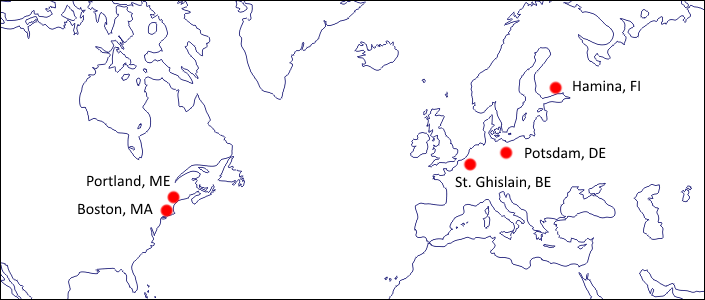
\includegraphics[width=0.7\textwidth]{figures/evaluation_and_results/usa_europe_map.png}
	\caption{Map of data center locations for day ahead price simulations}
	\label{fig:usa_europe_map}
\end{figure}

The locations have been chosen such that a diverse set of data from different energy markets is available. In addition time zone effects should be modeled by placing data centers sufficiently far from each other such that daily variation of energy prices in different time zones can be utilized. 

A list of day ahead energy markets and corresponding locations is shown in Table \ref{tab:list_of_day_ahead_markets}. 


\begin{table}[htbp]
\centering
\begin{tabular}{ll}
\toprule
 Energy market & Location \\
\midrule
	Nord Pool Spot &  Hamina, Finland \\
	Belpex &  St. Ghislain, Belgium \\
	EPEXSpot &  Potsdam, Germany \\
	ISO New England &  Portland, Maine \\
	ISO New England &  Boston, Massachussetts \\
\bottomrule
\end{tabular}
\caption{List of day ahead energy markets and locations}
\label{tab:list_of_day_ahead_markets}
\end{table}




\subsection{Real time simulation scenario}

For the real time simulation scenario data centers have been chosen exclusively from location within the US. Thus energy prices are more localized and performance of simulations should be evaluated for datasets with similar characteristics in contrast to day ahead simulations. 

A map showing data centers for all real time markets and locations is depicted in Figure \ref{fig:usa_map}. 

\begin{figure}[htbp]
	\centering
		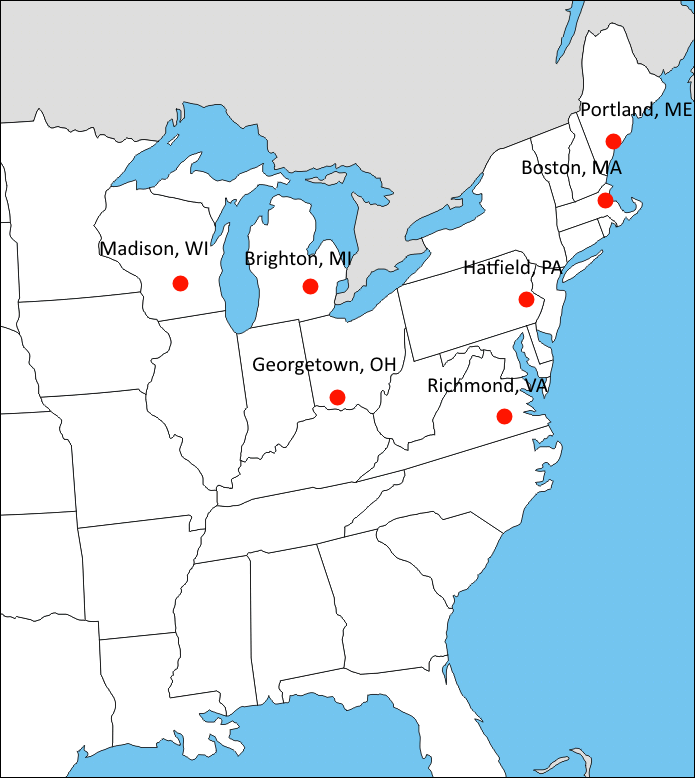
\includegraphics[width=0.50\textwidth]{figures/evaluation_and_results/usa_map.png}
	\caption{Map of data center locations for real time price simulations}
	\label{fig:usa_map}
\end{figure}

A list of real time energy markets and locations is outlined in Table \ref{tab:list_of_real_time_markets}. 

\begin{table}[htbp]
\centering
\begin{tabular}{ll}
\toprule
 Energy market & Location \\
\midrule
	ISO New England &  Portland, Maine \\
	ISO New England &  Boston, Massachussetts \\
	PJM & Richmond, Virginia  \\
	PJM & Brighton, Michigan  \\
	PJM & Hatfield, Pennsylvania  \\
	PJM & Madison, Wisconsin  \\
	PJM & Georgetown, Ohio  \\
\bottomrule
\end{tabular}
\caption{List of real time energy markets and locations}
\label{tab:list_of_real_time_markets}
\end{table}





\subsection{Simulation Configuration Parameters} \label{ssec:simulation_configuration_parameters}

\subsubsection{Cloud settings}

As the simulator has been built to be highly configurable \cite{lucanin2015philharmonic} different cloud parameters can be adjusted to run simulations with different settings. In Table \ref{tab:list_of_cloud_parameters} the most relevant simulation parameters are listed. 

\begin{table}[htbp]
\centering
\begin{tabularx}{\textwidth}{l|l|X}
	Metric & Values & Description \\
\hline
	number of servers & 500 & The total number of servers across all locations \\
	number of virtual machines & 5000 & The total number of virtual machines over the whole simulation time period \\
	server cpus & $[4,8]$ & The number of CPUs per server uniformly distributed over the given interval \\
	server memory & $[8,16]$ & The amount of memory per server uniformly distributed over the given interval \\
	virtual machine cpus & $[1,4]$ & The number of CPUs per VM uniformly distributed over the given interval \\
	virtual machine memory & $[1,4]$ & The amount of memory per VM uniformly distributed over the given interval \\
	dirty page rate & $\{20,40,70,90\}$ & One of four dirty page rates in MB/s assigned to each VM \\
	SLA level & 99.95\% & A fixed SLA availability level applied to each VM \\
	VM duration & $\{1,2,5,8,12,24,48\}$ & A fixed set of duration values in hours applied uniformly to the set of VMs \\
	VM price & 4 \cent \ / h & The price of a VM in cent per hour \\
	bandwidth & $\{400,800,1000\}$ & One of 3 amounts of bandwidths in MBit/s set between each two locations \\
	bandwidth cost & 0.1 \cent \ / GB & Bandwidth costs in cent per GB \\
	server peak power & 200 W & The power a server draws when its resources are fully utilized \\
	server idle power & 100 W & The power a server draws when idle \\
	cpu resource weight & 0.7 & The weight associated with cpu power when calculating server utilization \\
	memory resource weight & 0.3 & The weight associated with memory when calculating server utilization \\
\end{tabularx}
\caption{List of cloud configuration parameters in the simulation}
\label{tab:list_of_cloud_parameters}
\end{table}

The number of servers and VMs per simulation has been adjusted such that the resulting utilization is reasonable, e.g.~with 1000 servers and 2000 VMs in total an average utilization of only about 1 \% has been achieved over a simulation period of 5 weeks. Thus raising the number of VMs and in turn reducing number of servers led to a more realistic utilization of 30\% to 40\%. 

The relation of number of resources per server to the amount of VM resources (i.e.~number of cpus, memory) has been defined such that capacity constraints will not be an issue in simulations. The same method has been applied to the relation of total number of servers to number of VMs. 

The dirty page rate has a direct impact on VM migration performance (see Section \ref{sec:modeling_migration_energy}) and therefore different values have been assigned to VMs to simulate different application behavior. In combination with bandwidth this may lead to a high variation in migration downtimes. 

The SLA level has been set to the most common value for internet cloud services \cite{google2015compute,amazon2013sla}. With different penalty levels greater downtimes directly impact resulting costs for cloud providers. 

A different set of duration values has been assigned to VMs in order to simulate different kinds of workloads. This includes VM durations of 1 to 48 hours for scientific or HPC applications. Long running VMs have been omitted to focus on short term applications. 

The VM price most resembles the price for a ``n1-standard-1'' VM on Google Compute Cloud\footnote{\url{https://cloud.google.com/compute/pricing}}. As this is one of the smallest VMs available in the Google Cloud this price is still comparably cheap. 

Bandwidth is divided into low, medium and high values to simulate real world scenarios where high bandwidth may not always be available. As bandwidth has a direct impact on migration downtime this allows to evaluate the total resulting downtime and costs in different scenarios. 

Bandwidth costs have been set to a fixed price per amount of traffic while it is usually paid by fixed price contracts with 95/5 bandwidth constraints \cite{qureshi2009cutting}. These contracts measure traffic in fixed time intervals and the 95-th percentile of total usage is charged. To simplify the model in this work it has been set to a fixed price per volume. 

Server peak and idle power have been set where a server at peak load consumes double the amount of power than when idle. This may be too optimistic as it is stated that servers consume about 60\% of power when idle \cite{meisner2009powernap}. However studies show that new server technology is able to achieve power reductions up to 75\% from peak to idle mode \cite{prime2011energy}. 
A greater ratio of peak to idle power results in greater possibility for energy savings. Therefore the idle-to-peak ratio is critical for any scheduling algorithms aiming to reduce costs based on energy. 

CPU and memory resource weights have been defined to calculate resulting power consumption from server utilization of each resource. From investigations in \cite{meisner2009powernap,kansal2010virtual} it can be deduced that CPU is the most power consuming component where memory power consumption amounts to about one third up to equal amounts of CPU power. Therefore CPU and memory weights have been set to accommodate those findings. 



\subsubsection{Cloud scheduler} \label{sec:cloud_scheduler}

The core of the simulation is represented by the Cloud Scheduler. It is responsible for managing requests and for deciding which VMs should be migrated at which point in time. To make it a flexibel approach and be able to compare different scenarios the scheduler can be configured to run one out of seven different scenarios (Table \ref{tab:existing_scheduling_scenarios}). 


\begin{table}[htbp]
\centering
\begin{tabular}{lll}
\hline
  & \textbf{Request assignment} & \textbf{Migration handling} \\
\hline
	BFD baseline scheduler &  not cost aware, based on load & None \\
	BCF scheduler & cost aware, no forecasts & None \\
	BCF scheduler + FC & cost aware, forecasts & None \\
	BCF scheduler + Ideal FC & cost aware, ideal forecasts & None \\
	BCU scheduler + M & cost aware, no forecasts & cost aware, no forecasts \\
	BCU scheduler + M + FC & cost aware, forecasts & cost aware, forecasts \\
	BCU scheduler + M + ideal FC & cost aware, ideal forecasts & cost aware, ideal forecasts \\
\hline
\end{tabular}
\caption{Existing scheduling scenarios}
\label{tab:existing_scheduling_scenarios}
\end{table}

The first scheduler is a \textit{Best Fit Decreasing} (BFD) Scheduler that does no investigations on energy prices at all. It is based on a load balancing approach which aims to assign requests to the least occupied data center and utilize as few servers as possible to save energy costs. The BFD Scheduler is outlined in algorithm \ref{alg:bfd_scheduler}. 

The BFD scheduler iterates over the set of VM requests at the current point in time and aims to optimize placement of VMs by considering resource utilization of VMs and PMs for maximum consolidation. VM requests are sorted by resources in descending order to process VMs exhibiting large resource requirements first (line2). Locations are sorted by utilization ascending to assign requests first to under utilized locations (line 3). Lines 4 and 5 denote sorting of PMs by (free) capacities to consider most occupied servers first. 

\begin{algorithm}[htpb]
	\SetAlgoLined
	\SetKwProg{Fn}{Function}{:}{}
	\Fn{BFD Scheduler}{
		\KwData{Input Requests}
		\KwResult{Requests assigned according to BFD Schedule}
		sort VM requests with resource utilization in descending order\;
		sort locations by utilization in ascending order\;
		sort available PMs by location and free capacities in ascending order\;
		sort inactive PMs by capacities in ascending order\;
		
		\ForEach{vm in VM requests}{
			\While{vm not assigned {\normalfont and} size(available PMs) > 0}{
				\ForEach{pm in available PMs}{
					\If{vm fits on pm}{
						assign vm to pm\;
						remove vm from available PMs\;
						break\;
					}
				}
				
				\eIf{vm not assigned {\normalfont and} size(inactive PMs) > 0}{
					add first of inactive PMs to available PMs\;
					sort available PMs by location and free capacities ascending\;
				}{
					break\;
				}			
			}
		}
	}
\caption{Best fit decreasing scheduler}
\label{alg:bfd_scheduler}
\end{algorithm}

The BFD algorithm iterates over the set of requests and tries to assign VMs to hosts as long as non-fully occupied servers are available (line 7,8-14). In case a VM could not be assigned a server from the set of inactive hosts is activated and the aforementioned procedure is executed again (lines 15-17). In case no suitable host could be found or no further hosts are available the loop is exited with the current VM not being assigned (lines 18-19). 

As discussed before Table \ref{tab:existing_scheduling_scenarios} describes further scenarios with different scheduling algorithms. 
These algorithms are based on the \textit{Best Cost Fit} (BCF) and \textit{Best Cost Utility} (BCU) Scheduler with different variations to include migrations (denoted by \textit{M}), forecasts (denoted by \textit{FC}) and ideal forecasts (denoted by \textit{ideal FC}). 

The next discussed algorithm is the one from the Best Cost Fit scheduler which aims to maximize cost savings when assigning requests utilizing price forecasts. The corresponding algorithm is outlined in \ref{alg:bcf_scheduler}. 

\begin{algorithm}[htpb]
	\SetAlgoLined
	\SetKwProg{Fn}{Function}{:}{}
	\Fn{BCF Scheduler}{
		\SetKwInOut{Input}{Data}
    \SetKwInOut{Output}{Result}
		\Input{Input Requests \\
						flag for forecasts (FC)\\
						flag for ideal FC (idealFC)}
		\KwResult{Requests assigned according to BCF Schedule and given scenario}
		sort VM requests with resource utilization in descending order\;
		
		maxH <- 1\;
		\If{FC}{maxH <- get max fc horizon from config\;}
		
		\ForEach{vm in VM requests}{
			dur <- get remaining duration for vm\;
			\eIf{dur <= 1}
			{FC <- false\;idealFC <- false\;}
			{maxH <- min(dur,maxH)\;}
			
			fcData <- get sorted price and forecast data (FC, idealFC)\;
		
			\ForEach{data in fcData}{
				h <- get forecast horizon (data)\;
				loc <- get location (data)\;
				assign to host BFD (vm, loc)\;
				\If{assigned}{
					block vm for the next h time periods\;
					break\;
				}
			}
		}
	}
\caption{Best cost fit scheduler}
\label{alg:bcf_scheduler}
\end{algorithm}


The best cost fit scheduler takes three inputs: The VM requests, a flag denoting whether forecasts should be enabled and a second flag for possible inclusion of ideal forecasts. In line 2 requests are sorted descending by their resource requirements which resembles the step in the BFD scheduler. 

Lines 3-6 determine the maximum forecast horizon that should be taken into account when considering future energy prices (in case forecasts are enabled). From lines 7-11 the set of VM requests is iterated and forecasts are enabled based on the remaining duration. Line 13 determines the forecast horizon that will be applied through a minimum function of the remaining VM duration and the maximum forecast horizon defined previously. 

In line 15 a procedure is called to retrieve locations and best estimated forecast windows for these locations. Thus for each location and forecast horizon the average estimated energy price is calculated and results are sorted by price ascending such that the location with the least expected costs regarding a specific forecast horizon is placed first. 

\begin{algorithm}[htpb]
	\SetAlgoLined
	\SetKwProg{Fn}{Function}{:}{}
	\Fn{BCU Scheduler}{
		\SetKwInOut{Input}{Data}
    \SetKwInOut{Output}{Result}
		\Input{Input Requests \\
						Current cloud state \\
						flag for forecasts (FC)\\
						flag for ideal FC (idealFC)}
		\KwResult{A list of VMs with resulting utility value above the utility threshold}
		[slaPen,migEnergy,maxMigEnergy,remDur,maxRemDur,util,estimatedSavings] <- prepare utility function (FC, idealFC)\;
		
		uResult <- []\;
			
		\ForEach{vm in VM requests}{
		
			currentLoc <- getLocation(vm)\;
			uValue <- []\;
		
			\ForEach{loc in locations}{
				\If{loc != currentLoc}{
					
					slaPenalty <- 1 - slaPen[vm][loc]\;
					migrationEnergy <- 1 - (migEnergy[vm][loc] / maxMigEnergy)\;
					remainingDur <- remDur[vm] / maxRemDur\;
					dcLoad <- getRelativeDCLoad (util, currentLoc)\;
					costSavings <- estimatedSavings[vm][loc]\;
					
					result <- wSLA * slaPenalty + wMig * migrationEnergy + wDur * remainingDur + wLoad * dcLoad + wCost * costSavings\;
					
					uValue [loc] <- result\;
				}	
			}
			
			maxUValue <- max(uValue)\;
			append (uResult, (vm, getLocation(maxUValue), getUtilityValue(maxUValue)))\;
		}
		
		sort uResult by utility value descending\;
		result <- []\;
		uTH <- get utility TH from config ()\;
		
		\ForEach{r in uResult}{
			\If{utilityValue(r) > uTH}{
				append (result, r)\;
			}
		}
		
		return result\;
	}
\caption{Best cost utility scheduler}
\label{alg:bcu_scheduler}
\end{algorithm}

In lines 16 to 24 the resulting dataset from line 15 is iterated and the forecast horizon and location from the cheapest to more expensive locations are retrieved. For each of these data it is tried to assign the VM to a host from the given location based on a BFD approach. If the VM could be assigned successfully the VM will be blocked for migrations for the next $h$ time periods to prevent oscillation of VMs between different locations. 

The last scheduler is the Best Cost Utility Scheduler that takes into account VM migrations between different locations based on a utility function (see Section \ref{ssec:cloud_scheduler_and_utility_function} for a definition of the utility function). 
The algorithm of the BCU scheduler is shown in \ref{alg:bcu_scheduler}. 

Line 2 of the algorithm calls the procedure \textit{prepare utility function} that returns a list of metrics depending on the flags \textit{FC} and \textit{idealFC}. Results of utility calculations are stored in \textit{uResult} in line 3. 

From lines 4-6 start iterating over the set of VM requests and prepare the current location and a list of utility values. In addition lines 7 and 8 start iterating over the set of locations where the current location is skipped for migration. From line 9 to 13 the different criteria values are normalized from the results of the procedure in line 2. A list of criteria regarding this utility function can be found in Section \ref{ssec:cloud_scheduler_and_utility_function}. 

In line 14 the total utility value is calculated where each normalized criteria is weighted with its corresponding weight. The total utility value  is stored in line 15 for the current VM \textit{vm} and location \textit{loc}. Line 18 calculates the maximum utility value for this VM over all locations. That is, the most promising location where VM \textit{vm} could be migrated to is estimated. 

In line 19 a tuple consisting of \textit{(vm, loc, uvalue)} is added to the result utility list where \textit{uvalue} is the maximum of the calculated utility values for VM \textit{vm} associated with location \textit{loc}. 
Line 21 sorts the result utility list by utility value descending and line 22 and 23 are preparing the final result list and the utility threshold, which is taken from a configuration file. 

Lines 24 to 28 iterate over the resulting utility list and add values to the final result list in case the corresponding utility value exceeds the predefined utility threshold \textit{uTH}. 
The algorithm is concluded by returning the list of result VMs with total utility values above the utility threshold in line 29. 



\subsection{Cost models} \label{ssec:cost_model_definitions}

Cost models and related metrics are an important base for transforming aggregated power values to actual costs. Therefore a number of formulas have been defined to accurately model the resulting power consumption and energy costs. 
%These formulas are outlined below. 

\paragraph{Utilization of servers}
The basis for modeling power consumption is to define resource utilization of servers since server utilization relates directly to resulting power consumption \cite{meisner2009powernap}. 
Server utilization based on a set of resources $R$ is defined in Equation \ref{eq:server_utilization}. 

\begin{equation}
	s_{util}(t) = \sum_{r \in R} w_r \frac{s_{used}(r,t)}{s_{cap}(r)}
	\label{eq:server_utilization}
\end{equation}

with $w_r$ denoting the weight of resource $r$, $s_{used}$ is the currently used capacity of server $s$ regarding resource $r$ at time $t$, $s_{cap}$ denotes the total capacity of server $s$ of resource $r$ and $s_{util}$ being the resulting utilization of the server. 


\paragraph{Utilization per location}
In order to calculate data center load for each location a method of computing the average utilization per location is needed. 
It is defined as the average utilization of all servers in a given location (Equation \ref{eq:utilization_per_location}): 

\begin{equation}
	util_{loc}(t) = \frac{1}{|loc_{s}|} \sum_{s \in loc_{s}} s_{util}(t)
\label{eq:utilization_per_location}
\end{equation}

where $loc_{s}$ being the set of servers at location $loc$ and $util_{loc}$ denotes the current utilization at location $loc$. 


\paragraph{Power per location}

From the previous metric \textit{utilization per location} the resulting cloud power per location can be derived (Equation \ref{eq:power_loc}). 

\begin{equation}
	power_{loc}(t) = util_{loc}(t) \cdot |loc_{active_s}(t)| \cdot (P_{peak} - P_{idle}) + |loc_{active_s}(t)| \cdot P_{idle}
\label{eq:power_loc}
\end{equation}

where $|loc_{active_s}(t)|$ is the number of active servers at location $loc$ at time $t$, $P_{peak}$ is the peak power of the server and $P_{idle}$ describes the idle power of the server. 

\paragraph{Total cloud power}

The total cloud power is the sum of power consumption over all locations $L$ and time periods $T$ (Equation \ref{eq:m_tcp}). 

\begin{equation}
	m_{TCP} = \sum_{t \in T} \sum_{loc \in L} power_{loc}(t)
\label{eq:m_tcp}
\end{equation}


\paragraph{Migration load}
This metric serves as the basis for calculating migration energy as it directly depends on migration load. In addition it is used for further metrics such as migration costs. The formula for aggregated migration load per time $t$ is outlined in Equation \ref{eq:migration_load}.

\begin{equation}
	mig_l(t) = \sum_{v \in VM} V_{mig}(v,t)
\label{eq:migration_load}
\end{equation}

where $VM$ denotes the set of all active VMs at time $t$ and $V_{mig}(v,t)$ is the total migration load for vm $v$ for a migration starting at time $t$. The latter expression is taken from the definition of migration energy in Section \ref{sec:modeling_migration_energy}. 

\paragraph{Migration energy}
Modeling migration energy is needed for calculating the migration costs and it may also give a hint for resulting downtime and possible penalty costs due to the amount of migration energy consumed. 
The formulas for summed migration energy over the set of all VMs $VM$ and total migration energy over a simulation time period are denoted in Equations \ref{eq:migration_energy_by_time} and \ref{eq:migration_energy_total}. 

\begin{align}
	mig_e(t) = \sum_{v \in VM} E_{mig}(v,t) \label{eq:migration_energy_by_time}\\
	m_{ME} = \sum_{t \in T} mig_e(t) \label{eq:migration_energy_total}
\end{align}

\paragraph{Migration cost}
The migration costs are defined on the one side by combining resulting migration energy with current energy prices and on the other side by combining migration load and bandwidth costs. 

\begin{align}
	p_{mean}(t) &= \frac{p_{l1}(t) + p_{l2}(t)}{2} \label{eq:p_mean} \\
	mig_c(t) &= mig_e(t) \cdot p_{mean}(t) \label{eq:mig_c} \\
	mig_{c_{bw}}(t) &= mig_l(t) \cdot c_{bw} \label{eq:mig_c_bw} \\
	m_{MC} &= \sum_{t \in T} \left( mig_c(t) + mig_{c_{bw}}(t) \right) \label{eq:m_mc} 
\end{align}

Equation \ref{eq:p_mean} shows the mean price calculated from prices $p_{l1}$ and $p_{l2}$ in locations $l1$ and $l2$ at time $t$. 
Equation \ref{eq:mig_c} describes the migration costs depending on the migration energy and mean energy price $p_{mean}$ at time $t$. 
The bandwidth related costs for migration are outlined in Equation \ref{eq:mig_c_bw} with migration load and bandwidth costs combined (i.e.~amount of GB multiplied by \cent \ / GB). The migration cost metric $m_{MC}$ in Equation \ref{eq:m_mc} is then the sum of both energy and bandwidth costs. 

\paragraph{Cost of VM}
The resulting costs $v_c$ for a user of a VM is defined as the price $v_p$ set for the VM multiplied by its duration up to time $t$ (Equation \ref{eq:cost_of_vm}). 

\begin{equation}
	v_c(t) = v_p \cdot v_{dur}(t)
\label{eq:cost_of_vm}
\end{equation}

\paragraph{Penalty cost}

The total penalty costs are the aggregated costs for all penalties and VMs occurred during a simulation. Penalty costs occur when the maximum allowed downtime for a VM regarding an SLA threshold is exceeded. Depending on the threshold that has been surpassed different penalty costs have to be paid. 
As described in Section \ref{sec:sla_managemenet} three different penalty thresholds are defined which result in different penalty costs. 

\begin{align}
	SLA_{TH_i}(v,t) &= v_{dur}(t) \left( 1 - \frac{v_{SLA_i}}{100} \right), i \in \{1,2,3\} \label{eq:sla_th_i} \\
	v_{SLA_1} &= 99.95, v_{SLA_2} = 99, v_{SLA_3} = 95 \label{eq:sla_levels} \\
	v_{pen}(t) &= \left\{
								\begin{array}{@{}ll@{}}
									0.5, & \text{if } down_{acc}(v,t) > SLA_{TH_3}(v,t) \\
									0.25, & \text{if } down_{acc}(v,t) > SLA_{TH_2}(v,t) \\
									0.1, & \text{if } down_{acc}(v,t) > SLA_{TH_1}(v,t) \\
									0, & \text{otherwise}
								\end{array}\right. \label{eq:v_pen}  \\
	v_{c_{pen}}(t) &= v_c(t) \cdot v_{pen}(t) \label{eq:v_c_pen} \\
	m_{TPC} &= \sum_{v \in VM} v_{c_{pen}}(t_{last}) \label{eq:m_pc} 
\end{align}

Equation \ref{eq:sla_th_i} defines an SLA threshold for either of the defined SLA levels in Equation \ref{eq:sla_levels}. In Equation \ref{eq:v_pen} penalty values in the interval [0,1] are assigned based on the SLA threshold reached. This penalty value is then applied to the costs of the VM in Equation \ref{eq:v_c_pen} resulting in penalty costs for VM $v$. Equation \ref{eq:m_pc} calculates the total penalty costs across all VMs at the last simulation time stamp $t_{last}$. 


\paragraph{Total downtime}

The total downtime is calculated from the sum of downtimes of all VMs over the whole simulation time period (up to $t_{last}$, Equation \ref{eq:m_tdt}). 

\begin{equation}
	m_{TDT} = \sum_{v \in VM} down_{acc}(v,t_{last})
\label{eq:m_tdt}
\end{equation}

\paragraph{Number of migrations}

The total number of migrations is defined as the sum of migrations at each time stamp $t$ (Equation \ref{eq:num_migrations}). 

\begin{equation}
	m_{NM} = \sum_{t \in T} mig_{num} (t) 
\label{eq:num_migrations}
\end{equation}

where $mig_{num}(t)$ denotes the number of migrations at time $t$. 


\paragraph{Total cloud costs}

The total cloud costs are calculated as the sum of cloud power values multiplied by the price at the respective location and time (Equation \ref{eq:m_tcc}). 

\begin{equation}
	m_{TCC} = \sum_{t \in T} \sum_{loc \in L } power_{loc}(t) \cdot p_{loc}(t)
\label{eq:m_tcc}
\end{equation}

\paragraph{Total cloud power with migrations}

Calculating the total cloud power including migrations is a simple addition of the total cloud power and migration energy (Equation \ref{eq:m_tcpwm}). 

\begin{equation}
	m_{TCPWM} = m_{TCP} + m_{ME}
\label{eq:m_tcpwm}
\end{equation}

\paragraph{Total cloud cost with migrations}

Analogously to \textit{Total power with migrations} this metric is defined as the sum of total cloud cost and migration cost (Equation \ref{eq:m_tccwm}). 

\begin{equation}
	m_{TCCWM} = m_{TCC} + m_{MC}
\label{eq:m_tccwm}
\end{equation}

\paragraph{Total power}

The total power metric encompasses the metric \textit{Total cloud power with migrations} to describe the total power consumption in the simulation (Equation \ref{eq:m_tp}). 

\begin{equation}
	m_{TP} = m_{TCPWM}
\label{eq:m_tp}
\end{equation}

\paragraph{Total cost}

Total cost denote the sum of all cost occurred during simulation which includes the total cloud cost with migrations plus total penalty costs (Equation \ref{eq:m_tc}). 

\begin{equation}
	m_{TCCWM} = m_{TCCWM} + m_{TPC}
\label{eq:m_tc}
\end{equation}









\section{Utility function optimization} \label{sec:utility_function_optimization}

As explained in Section \ref{sec:cost_optimization_based_on_utility_function} the scheduler incorporates a utility function to provide a means of flexibel adjustments to different cloud criteria. This section aims to optimize the parameters of the utility function regarding both energy cost savings and SLA penalties. The resulting settings will then be used in large scale simulations which will be presented in Section \ref{sec:simulation_results}. 

In the following simulations the scheduler operates on the defined cloud parameters in Section \ref{ssec:simulation_configuration_parameters}. 
For the utility test scenarios outlined in this section the number of servers and VMs is changed to a total of 1000 servers and 2000 VMs over the whole simulation time period. This gives sufficient opportunity to test the utility function but does not require huge computational resources. 

The simulation runs in this section are based on 5 weeks of energy price data from day ahead markets with locations defined in Section \ref{sec:definition_of_simulation_scenarios}. As a common setting to these simulations the following bandwidth connections have been defined for day ahead scenarios between locations (Table \ref{tab:bandwidth_connections_in_da_markets}). To simplify the scenario all bandwidth connections are symmetric, i.e.~the same in- and outgoing bandwidth connections have been used between each two locations. 


\begin{table}[htbp]
\centering
\begin{tabular}{lll}
\toprule
	Source & Destination & Bandwidth \\
\midrule
	Hamina & Potsdam & 1000 MBit/s \\
	Hamina & St. Ghislain & 800 MBit/s \\
	Potsdam & St. Ghislain & 800 MBit/s \\
	Boston & Portland & 800 MBit/s \\
	Europe & USA & 400 MBit/s \\
\bottomrule
\end{tabular}
\caption{Bandwidth connections in day ahead market locations}
\label{tab:bandwidth_connections_in_da_markets}
\end{table}

The connection Europe to USA denotes connections from any country from Europe to any country in the USA which is mapped to 400 MBit/s. 

In order to easily distinguish between different schedulers a characterizing symbol has been introduced to designate each scheduler. The resulting mapping is shown in Table \ref{tab:scheduler_name_mapping}.

\begin{table}[htbp]
\centering
\begin{tabular}{lll}
\toprule
  Scheduler name & Symbol \\
\midrule
	BFD baseline scheduler & BFD \\
	BCF scheduler & BCF \\
	BCF scheduler + FC & BCF\_F \\
	BCF scheduler + Ideal FC & BCF\_IF \\
	BCU scheduler + M & BCU\_M \\
	BCU scheduler + M + FC & BCU\_MF \\
	BCU scheduler + M + ideal FC & BCU\_MIF \\
\bottomrule
\end{tabular}
\caption{Existing scheduling scenarios}
\label{tab:scheduler_name_mapping}
\end{table}


For a reference of all implemented cloud metrics shown in subsequent graphs these metrics are outlined in Table \ref{tab:list_of_cloud_metrics} (see also Section \ref{ssec:cost_model_definitions}). 


\begin{table}[htbp]
\centering
\begin{tabularx}{\textwidth}{llX}
\toprule
  Cloud metric & Symbol & Description \\
\midrule
	Total cloud power & TCP & The total power consumed by active servers aggregated over all locations and time periods \\
	Total cloud cost & TCC & The total costs resulting from applying energy prices to power consumption over the simulation time period \\
	Migration energy & ME & Migration energy summed up from all migrations over the simulation time period \\
	Migration cost & MC & Migration costs summed up from all migrations over the simulation time period \\
	Total cloud power & TCPWM & The total cloud power including the migration energy \\
	with migrations & & \\
	Total cloud cost & TCCWM & The total cloud costs including the resulting migration \\
	with migrations & & costs \\
	Total penalty cost & TPC & Total penalty costs occurred during the simulation time period \\
	Total downtime & TDT & Total downtime aggregated over the simulation time period \\
	Number of migrations & NM & Number of migrations triggered over the simulation time period \\
	Total power & TP & The total cloud power including the migration energy \\
	Total cost & TC & The total cloud costs including migration costs and total penalty costs \\
\bottomrule
\end{tabularx}
\caption{List of all measured cloud metrics}
\label{tab:list_of_cloud_metrics}
\end{table}

As might be noticed the metrics \textit{Total cloud power with migrations} and \textit{Total power} are defined the same since on the one side no more power values are to be added and on the other side a total metric comparable to the \textit{Total cost} should to be defined. 


In the following sections three different scenarios are defined to show the impact of changing utility parameters on resulting costs and SLA penalties.

\subsection{Scenario1: Energy utility function}

The first scenario consists of parameters to emphasize the reduction of migration energy consumption whereby less weights have been put on prevention of SLA penalties. 
The utility criteria and corresponding weights are outlined in Table \ref{tab:list_of_energy_utility_criteria_weights}. 

\begin{table}[htbp]
\centering
\begin{tabular}{lll}
\toprule
	Index & Name of criterion	& weight \\
\midrule
	$c_1$ & probability of SLA penalty & 0.4 \\
	$c_2$ & estimated migration energy & 0.7 \\
	$c_3$ & remaining VM duration & 0.5 \\
	$c_4$ & data center load & 0.4 \\
	$c_5$ & estimated cost benefit & 0.8 \\
	$ut$ & utility threshold & 1.8 \\
\bottomrule
\end{tabular}
\caption{List of energy utility criteria with associated weights}
\label{tab:list_of_energy_utility_criteria_weights}
\end{table}

We can observe that the \textit{estimated cost benefit} and \textit{estimated migration energy} criteria have been given the highest weights whereas other criteria such as \textit{probability of SLA penalty} are set to lower weights. 
The utility threshold value of 1.8 is the minimum value that has to be reached by a VM's utility function for the VM to be considered eligible for migration. 

Since all criteria values are normalized to the interval $[0,1]$ it can be quite easily estimated which values of the different criteria lead to utility values above the utility threshold. A trivial method of estimating utility weights is to set all criteria values to 1 and calculate the sum of their weights. This should result in a value signficantly greater than the utility threshold. One could also put particularly high emphasis on one criterion by keeping the sum of weights of all other criteria below the weight of this criterion. Then by setting the utility threshold to a value at least as high as that specific criterion it is assured that a sufficiently high value of this criterion is required to get above the utility threshold. 

The results for normalized power vs cost values are depicted in Figure \ref{fig:energy_utility_power_vs_cost}. 

\begin{figure}[htbp]
	\centering
		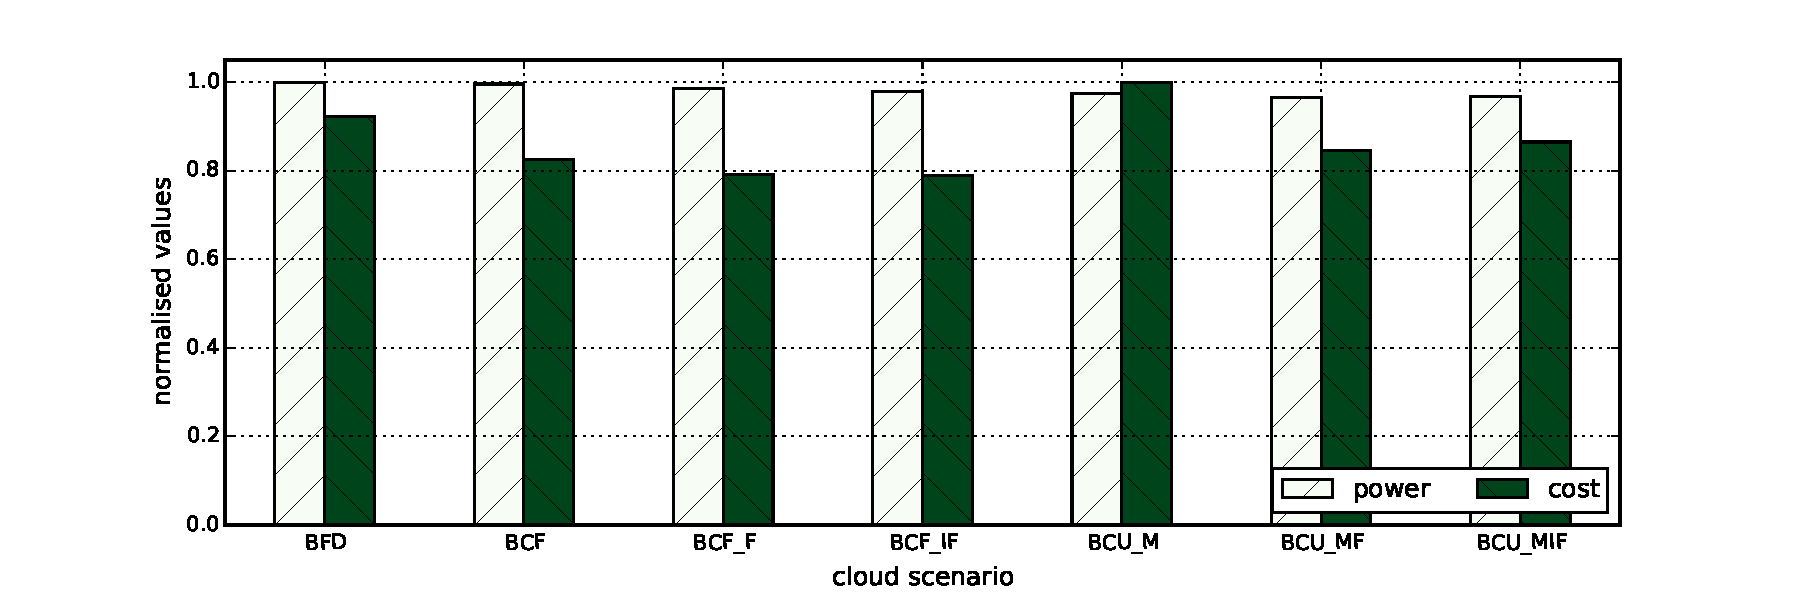
\includegraphics[width=1.00\textwidth]{figures/evaluation_and_results/energy_utility_power_vs_cost.pdf}
	\caption{Normalized cost vs power values based on the energy utility scenario}
	\label{fig:energy_utility_power_vs_cost}
\end{figure}

This graph outlines the resulting power and costs for this utility scenario across all defined schedulers (see Section \ref{sec:cloud_scheduler} for a definition of the schedulers). What can be observed is that power values differ only marginally while energy costs differ substantially between different schedulers. The BFD scheduler is taken as the baseline scheduler to which all other schedulers are compared. 

In this scenario the BFD scheduler exhibits the highest power consumption among all schedulers but less total costs than the BCU\_M scheduler. Overall the BCU schedulers (BCU\_M, BCU\_MF, BCU\_MIF) are not able to reduce costs as much as BCF schedulers (BCF, BCF\_F, BCF\_IF). Thus the utility function which is applied in BCU schedulers is not well calibrated. This behavior can be explained as we put on a high weight for the \textit{estimated cost benefit} criteria but a low weight on \textit{probability of SLA penalties} which allows the use of excessive migrations that can result in increased SLA penalty costs. 

The total resulting costs including migration costs and SLA penalty costs is shown in Figure \ref{fig:energy_utility_total_cost}. 
What is clearly visible are the added penalty and migration costs for the schedulers BCU\_M, BCU\_MF and BCU\_MIF. Therefore even though the cloud cost may be reduced compared to other schedulers the total costs are higher due to these additional costs. 

\begin{figure}[htbp]
	\centering
		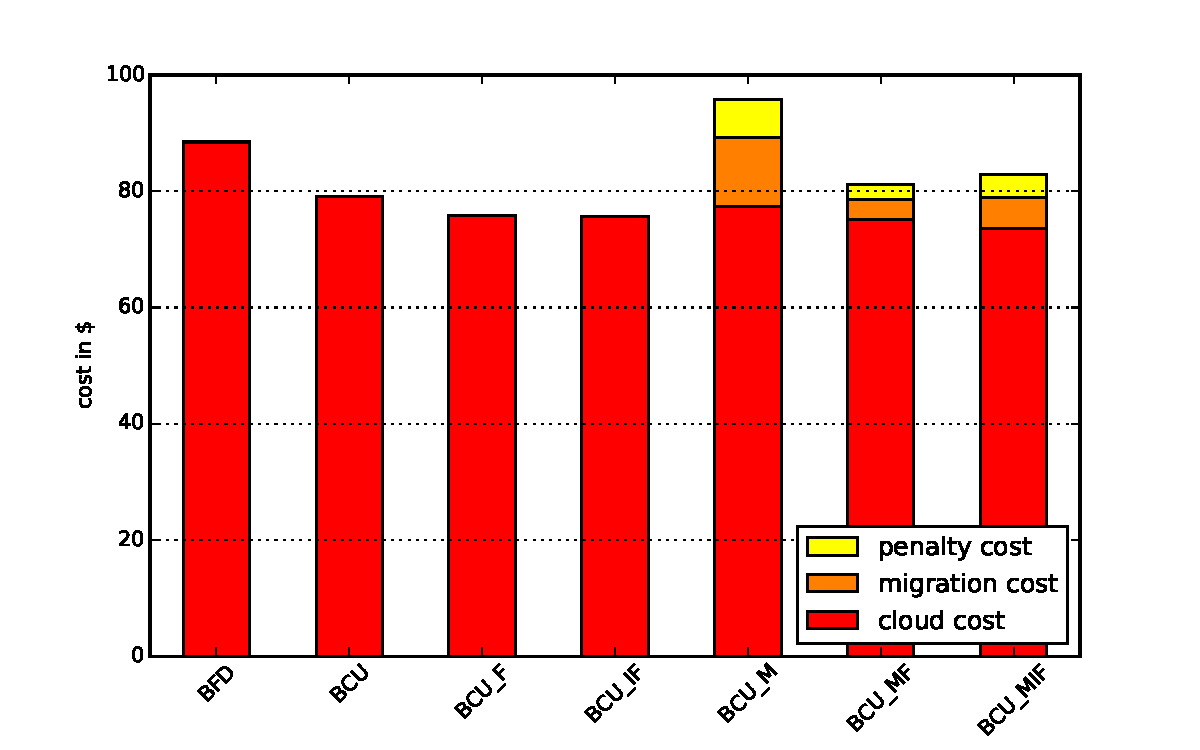
\includegraphics[width=0.7\textwidth]{figures/evaluation_and_results/energy_utility_total_cost.pdf}
	\caption{Total resulting costs per scheduler for the energy utility scenario}
	\label{fig:energy_utility_total_cost}
\end{figure}

A diagram summarizing all the cloud metrics is depicted in Figure \ref{fig:energy_utility_cloud_metrics}. For a list of cloud metrics see Table \ref{tab:list_of_cloud_metrics}. 

\begin{figure}[bp]
	\centering
	\hspace*{-1.6in}
		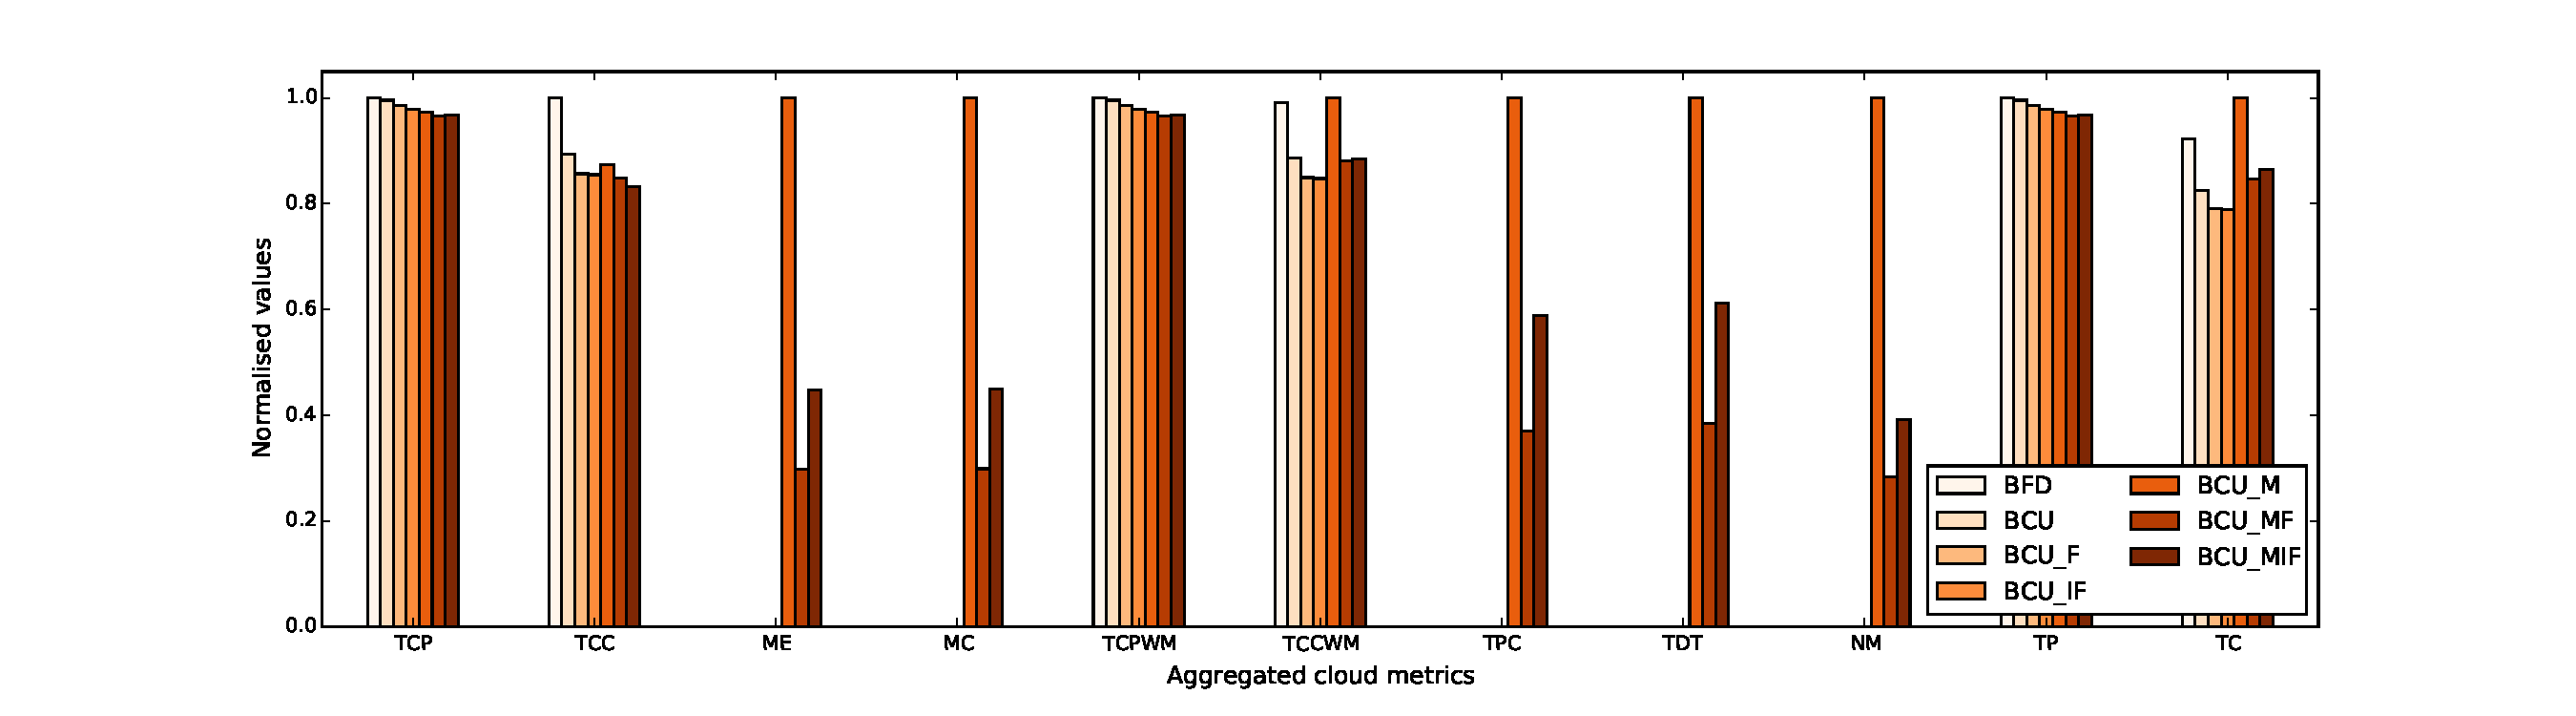
\includegraphics[width=1.50\textwidth]{figures/evaluation_and_results/energy_utility_cloud_metrics.pdf}
	\caption{Cloud metrics calculated for the energy utility over the simulation time period}
	\label{fig:energy_utility_cloud_metrics}
\end{figure}

This diagram shows normalized values of cloud metrics over the whole simulation time period. Significant deviations of values can be observed for different schedulers. The results coincide with the graphs shown before as total cloud power values decrease only marginally while total cloud costs are reduced significantly (i.e.~BFD scheduler compared to BCU\_MIF scheduler for metrics TCP and TCC). 

Since migration energy and migration costs are directly proportional the normalized values are exactly the same. They are highest for the BCU\_M scheduler and decrease for BCU\_MF and BCU\_MIF schedulers since the latter ones include forecasts in the calculations. Other schedulers do not exhibit any migration energy or costs since no migrations are performed. 

The total cloud power with migrations (TCPWM) is almost identical to the TCP metric since migration energy only accounts for a very small fraction of the total cloud power. The total cloud costs with migrations (TCCWM) show a significantly different behavior due to the addition of migration costs based mainly on bandwidth costs. 

In the total penalty cost (TPC) metric the BCU\_M scheduler exhibits the highest penalty costs. It shows a similar behavior to the TCCWM metric as higher migration costs and therefore a higher number of migrations generally lead to increased penalty costs. 
In accordance with the penalty costs and migration costs the total downtime shows similar patterns as penalty costs are directly related to VM downtime. 

The number of migrations (NM) metric again shows similar behavior as the aforementioned metrics all relate to the total number of migrations. The total power (TP) metric is identical to the TCPWM metric and shown on the right for easier comparison to the total cost (TC) metric. 

The total cost metric adds to the pattern of TCCWM as in addition to cloud and migration costs the penalty costs are taken into account. 
Thus it can be concluded that due to high migration and penalty costs the BCU schedulers result in increased costs compared to the BCF schedulers. 


\subsection{Scenario2: Cost utility function}

The cost utility function is defined as utility scenario 2 where the focus has been laid on high cost optimization with other metrics having low priority. 

In Table \ref{tab:list_of_cost_utility_criteria_weights} the weights for the cost utility function are displayed. 

\begin{table}[htbp]
\centering
\begin{tabular}{lll}
\toprule
	Index & Name of criterion	& weight \\
\midrule
	$c_1$ & probability of SLA penalty & 0.3 \\
	$c_2$ & estimated migration energy & 0.4 \\
	$c_3$ & remaining VM duration & 0.2 \\
	$c_4$ & data center load & 0.1 \\
	$c_5$ & estimated cost benefit & 1.0 \\
	$ut$ & utility threshold & 1.4 \\
\bottomrule
\end{tabular}
\caption{List of cost utility criteria with associated weights}
\label{tab:list_of_cost_utility_criteria_weights}
\end{table}

A very high value has been set for the \textit{estimated cost benefit} criterion equaling to the sum of all other criteria. The utility threshold has been set to a value higher than the sum of all criteria but the cost benefit, therefore this threshold cannot be reached without a significantly high value of the cost benefit. 

\textit{Probability of SLA penalty} and \textit{estimated migration energy} are weighted higher than other criteria but exhibit still a low value compared to the cost benefit. Thus it is expected that costs will be optimized with still a fraction existing for migration and penalty costs. 

The normalized cost vs power graph is shown in Figure \ref{fig:cost_utility_power_vs_cost}. 

\begin{figure}[htbp]
	\centering
		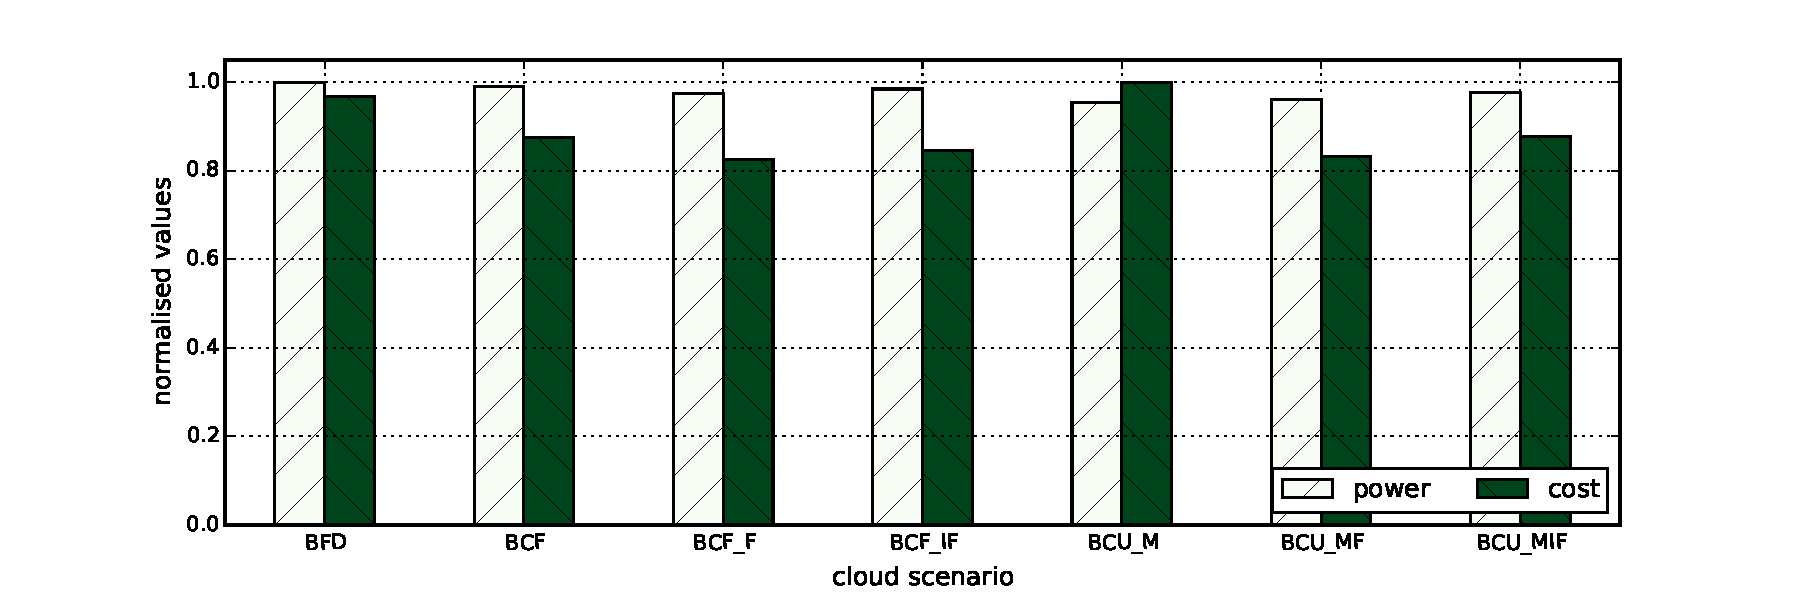
\includegraphics[width=1.00\textwidth]{figures/evaluation_and_results/cost_utility_power_vs_cost.pdf}
	\caption{Normalized cost vs power values based on the cost utility scenario}
	\label{fig:cost_utility_power_vs_cost}
\end{figure}

This graph shows more evenly distributed cost values than the one from scenario 1 (Figure \ref{fig:energy_utility_power_vs_cost}). Thus the BFD scheduler almost reaches the maximum cost value but the BCU\_M scheduler still shows the highest costs of all schedulers. It can be noticed that the BCU schedulers are at the same levels as BCF schedulers with the BCU\_MF scheduler showing only a minor increase in costs in comparison to the BCF\_F scheduler exhibiting the least costs. 

\begin{figure}[bp]
	\centering
		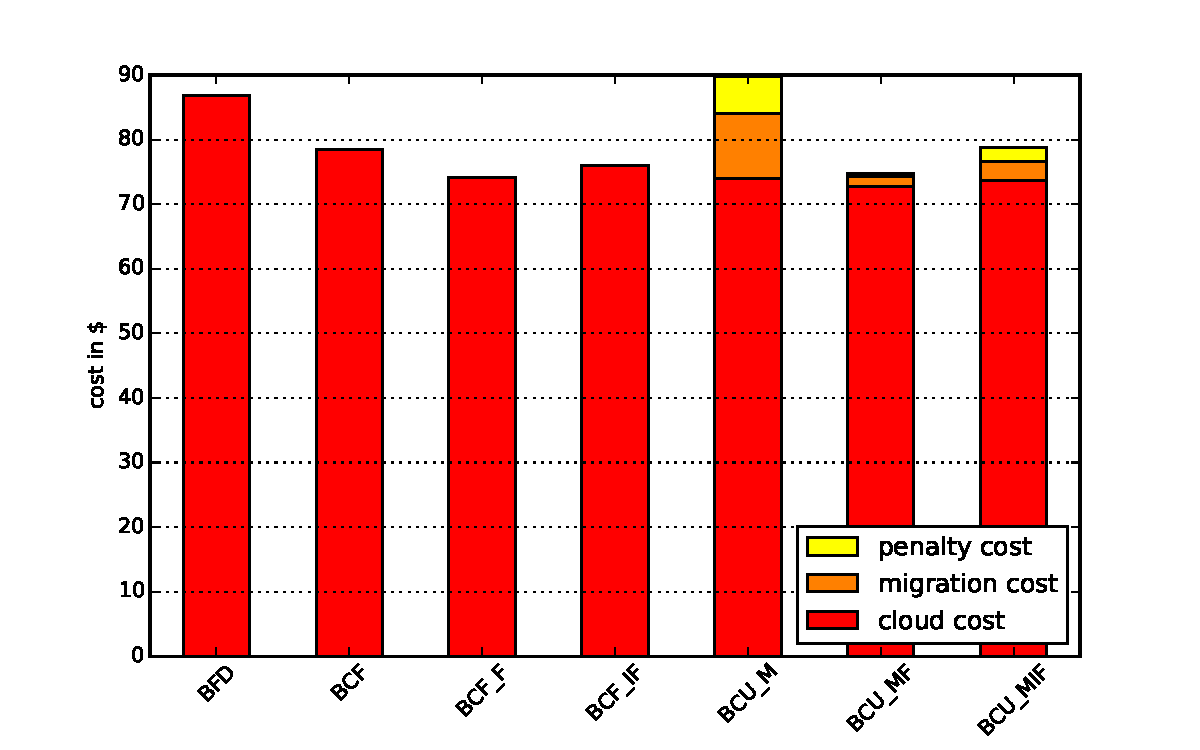
\includegraphics[width=0.7\textwidth]{figures/evaluation_and_results/cost_utility_total_cost.pdf}
	\caption{Total resulting costs per scheduler for the cost utility scenario}
	\label{fig:cost_utility_total_cost}
\end{figure}


The total costs are depicted in Figure \ref{fig:cost_utility_total_cost}. Compared to the total cost chart of scenario 1 (Figure \ref{fig:energy_utility_total_cost}) the total costs for all schedulers except the BFD scheduler have been reduced. Also the fraction of migration and penalty costs could be reduced except for the BCU\_M scheduler with a slight increase of penalty costs. 

In Figure \ref{fig:cost_utility_cloud_metrics} the resulting cloud metrics are shown. 

\begin{figure}[htbp]
	\centering
	\hspace*{-1.2in}
		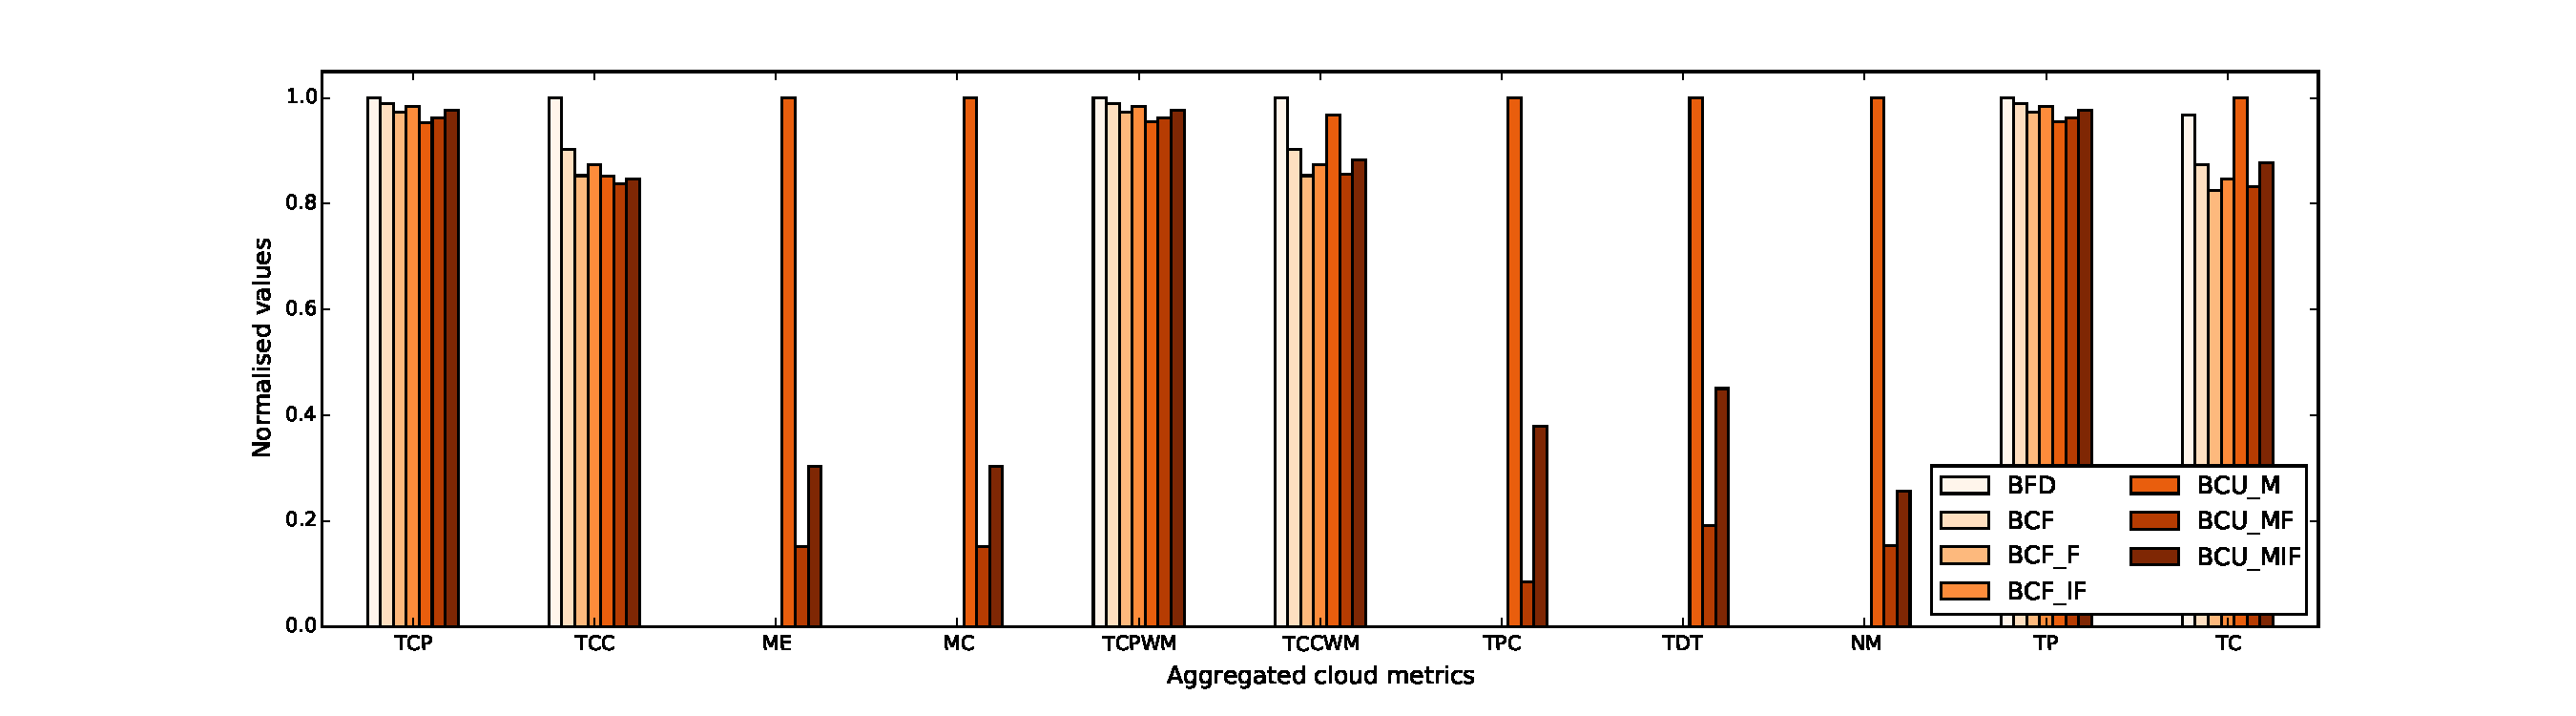
\includegraphics[width=1.50\textwidth]{figures/evaluation_and_results/cost_utility_cloud_metrics.pdf}
	\caption{Cloud metrics calculated for the cost utility over the simulation time period}
	\label{fig:cost_utility_cloud_metrics}
\end{figure}

The most obvious changes compared to the energy utility scenario are the decreased migration energy, migration cost, total penalty cost, total downtime and number of migration criteria (ME, MC, TPC, TDT and NM) for the BCU\_MF and BCU\_MIF schedulers in relation to the BCU\_M scheduler. 

Thus fewer migrations lead to fewer downtimes, SLA violations and penalties and also migration energy and costs. The reason that the latter two BCU schedulers perform significantly better than the BCU\_M scheduler is the fact that the \textit{estimated cost benefit} metric has the most impact when applied to an extended time series with forecasts. 



\subsection{Scenario3: Best utility function} \label{ssec:best_utility_function}

The best utility function has been defined as the scenario with the highest cost savings compared to other scenarios. It puts emphasis on both reduction of SLA penalties as well as optimization of energy costs during the simulation. 

The defined weights assigned to the different criteria are denoted in Table \ref{tab:list_of_best_utility_criteria_weights}. 

\begin{table}[htbp]
\centering
\begin{tabular}{lll}
\toprule
	Index & Name of criterion	& weight \\
\midrule
	$c_1$ & probability of SLA penalty & 1.0 \\
	$c_2$ & estimated migration energy & 0.1 \\
	$c_3$ & remaining VM duration & 0.2 \\
	$c_4$ & data center load & 0.1 \\
	$c_5$ & estimated cost benefit & 1.0 \\
	$ut$ & utility threshold & 2.0 \\
\bottomrule
\end{tabular}
\caption{List of best utility criteria with associated weights}
\label{tab:list_of_best_utility_criteria_weights}
\end{table}

As can be observed the \textit{probability of SLA penalty} and \textit{estimated cost benefit} metrics are given the highest possible weights while other criteria are weighted almost negligibly. The utility threshold amounts to the sum of the two highest weights making sure that only VMs with high relative values for metrics $c_1$ and $c_5$ are considered for migrations. 

\begin{figure}[bp]
	\centering
		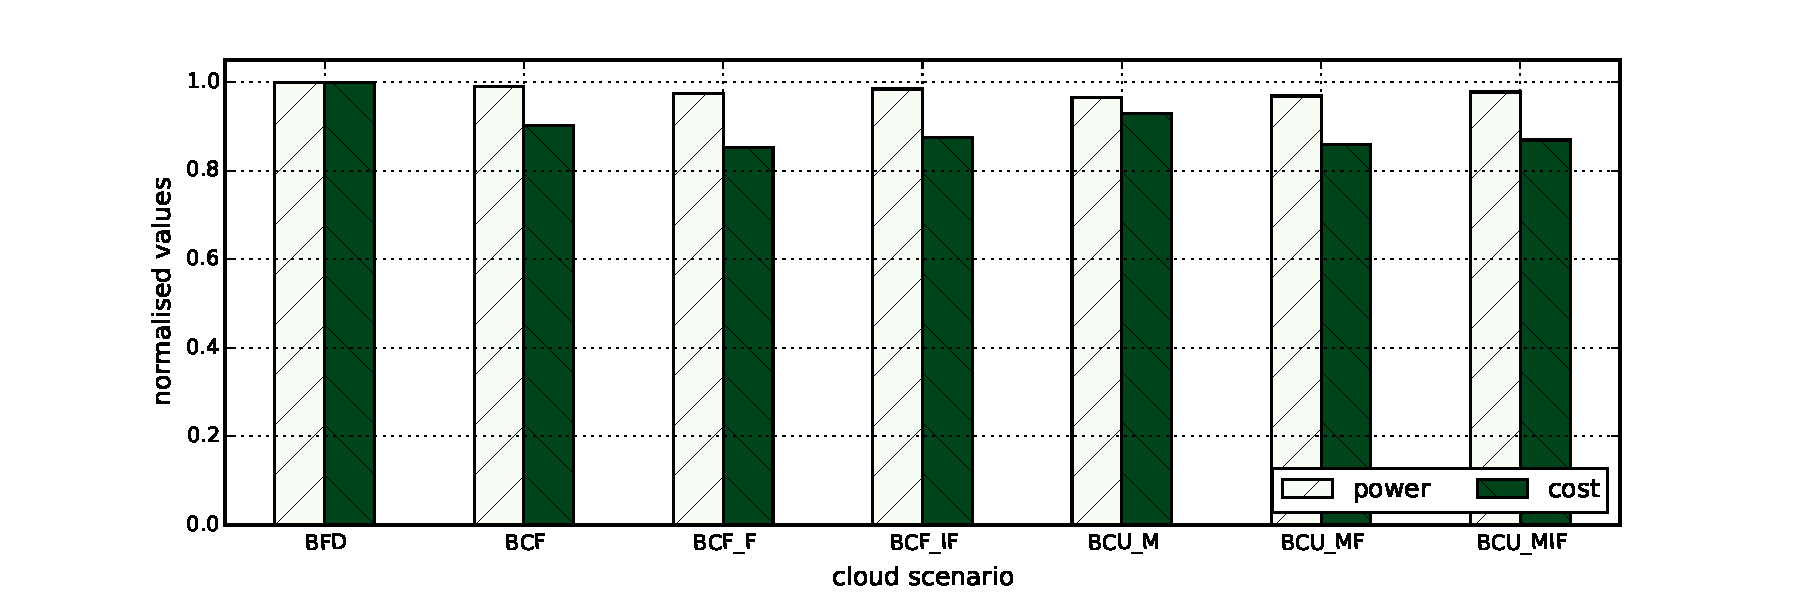
\includegraphics[width=1.00\textwidth]{figures/evaluation_and_results/best_utility_power_vs_cost.pdf}
	\caption{Normalized cost vs power values based on the best utility scenario}
	\label{fig:best_utility_power_vs_cost}
\end{figure}

The power vs cost chart is given in Figure \ref{fig:best_utility_power_vs_cost}. 
The normalized costs are more evenly distributed across the schedulers than for scenarios 1 and 2 (Figures \ref{fig:energy_utility_power_vs_cost} and \ref{fig:cost_utility_power_vs_cost}). The BCU\_M scheduler still shows higher costs compared to other schedulers except the BFD scheduler. 
Power values also show small deviations of up to 2\% where most energy savings can be achieved by the BCU\_M and BCU\_MF schedulers. 

Total costs are depicted in Figure \ref{fig:best_utility_total_cost}. No penalty costs have resulted for this scenario which coincides with the adjustments of utility weights where highest weights were put on \textit{probability of SLA penalty} and \textit{estimated cost benefit} criteria. 
Also total costs could be reduced for schedulers BCU\_M, BCU\_MF and BCU\_MIF. 

\begin{figure}[tbp]
	\centering
		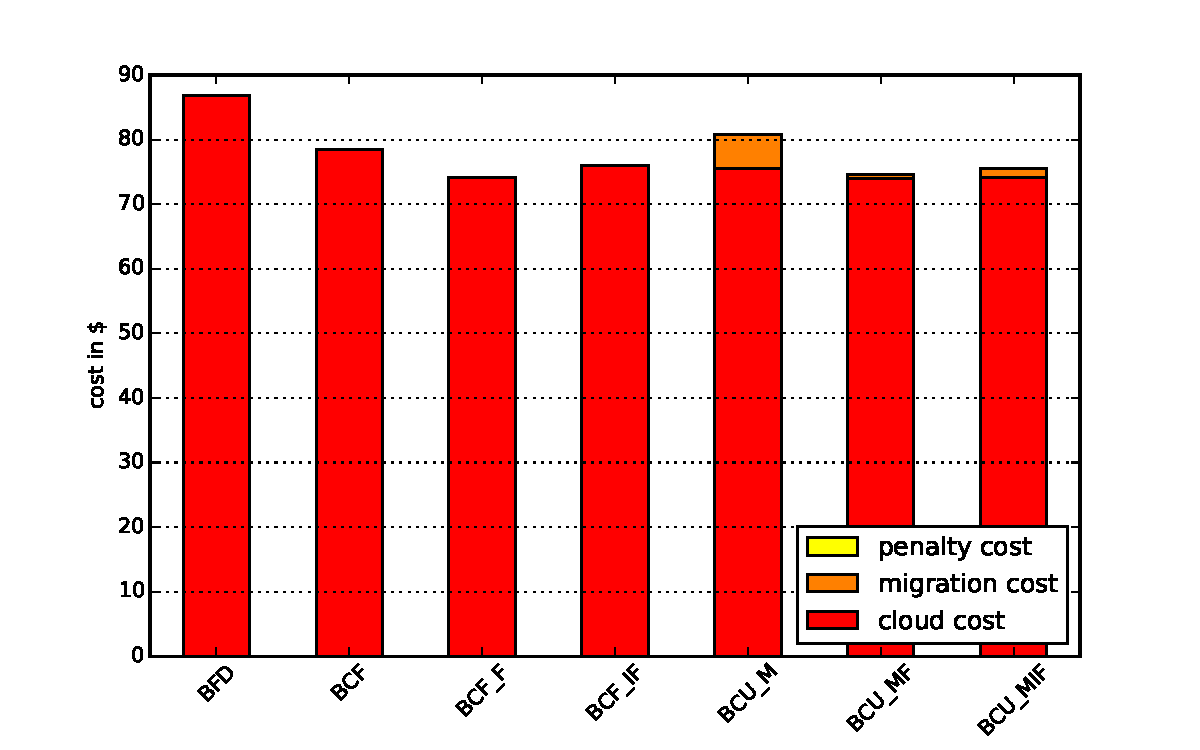
\includegraphics[width=0.7\textwidth]{figures/evaluation_and_results/best_utility_total_cost.pdf}
	\caption{Total resulting costs per scheduler for the best utility scenario}
	\label{fig:best_utility_total_cost}
\end{figure}

In Figure \ref{fig:best_utility_cloud_metrics} the resulting cloud metrics are shown. 

\begin{figure}[htbp]
	\centering
	\hspace*{-1.2in}
		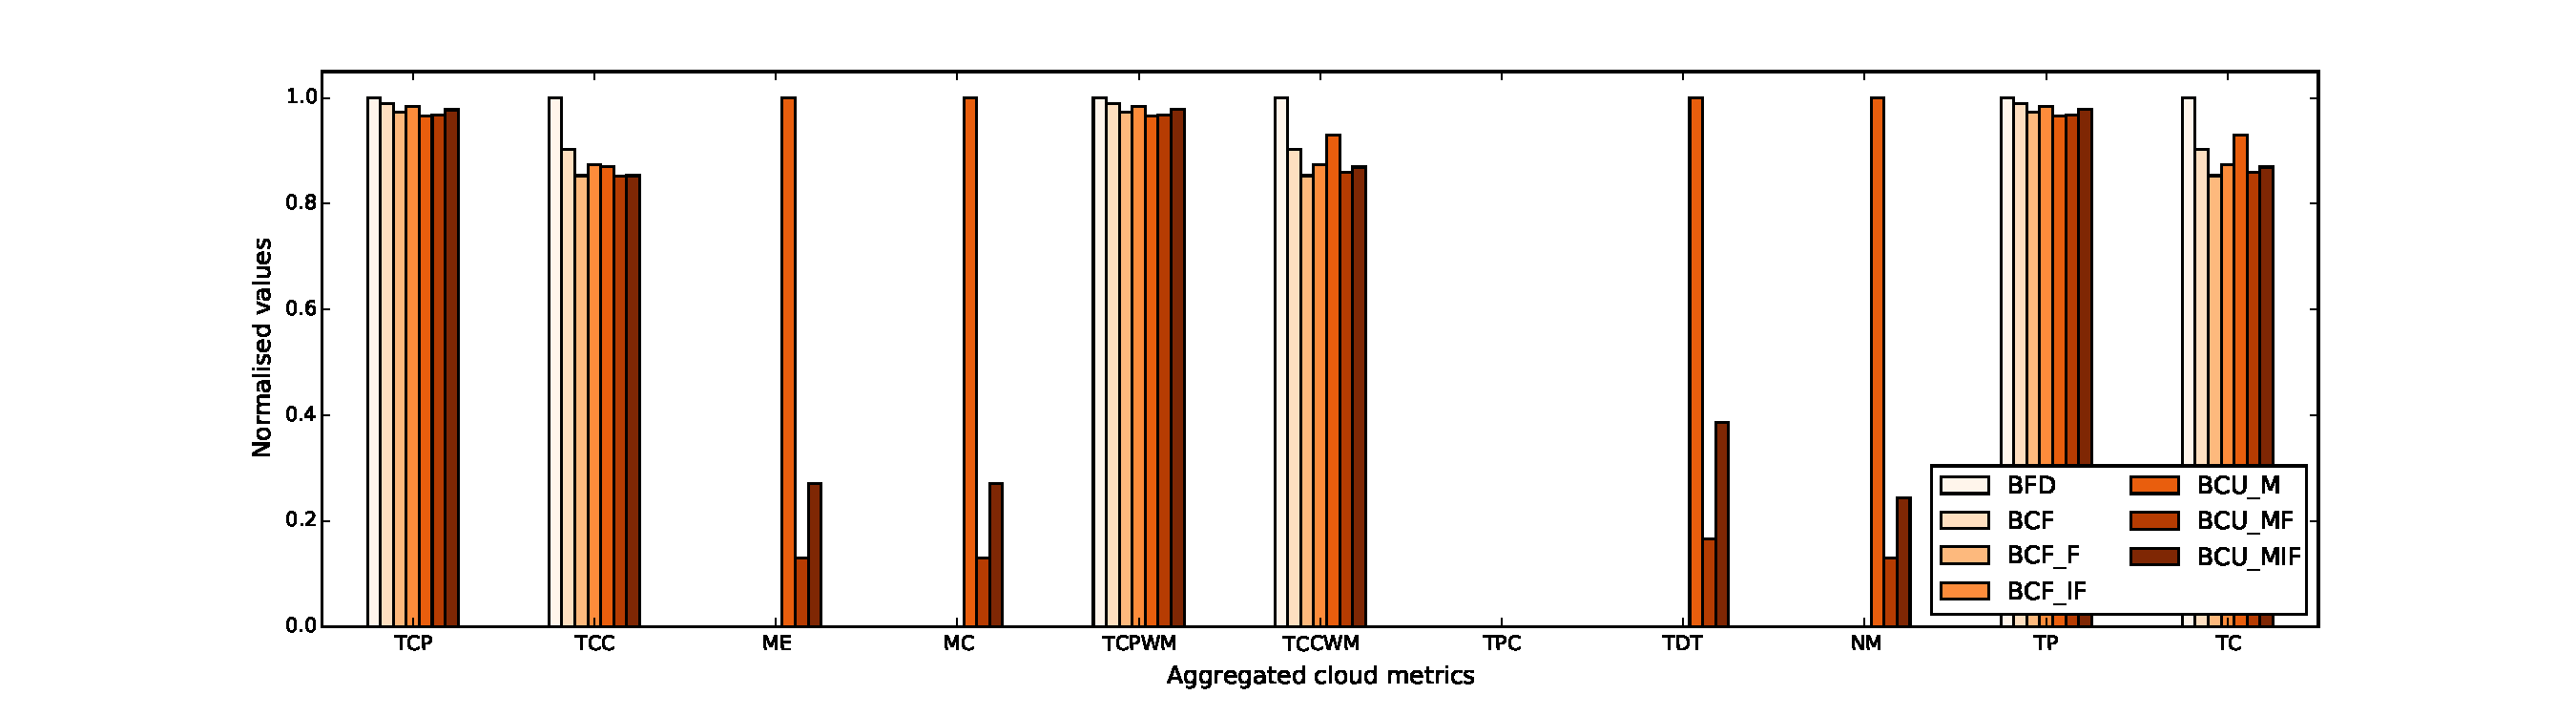
\includegraphics[width=1.50\textwidth]{figures/evaluation_and_results/best_utility_cloud_metrics.pdf}
	\caption{Cloud metrics calculated for the best utility over the simulation time period}
	\label{fig:best_utility_cloud_metrics}
\end{figure}

What can be deduced by this graph is that cost and migration dependent metrics (TCCWM, TPC, TC) show substantially reduced values where no penalty costs are shown at all (TPC). The ME, MC, TDT and NM metrics show lower values as well in relation to the BCU\_M scheduler. 
Other metrics such as power values do not exhibit significant variations however emphasis have been put on cost rather than power reductions. 

The resulting cost reductions for all scenarios are shown in Table \ref{tab:utility_evaluation_results}. 
Cost reductions of cost and best utility scenarios in percent compared to the energy utility scenario have been denoted as cost (\%) and best (\%), respectively. 
The best utility scenario exhibits the least total costs where substantial cost reductions of up to 15\% (BCU\_M scheduler) have been achieved. It also provides the highest cost reductions compared to the energy utility scenario with further reduced costs for the BCU\_M, BCU\_MF and BCU\_MIF schedulers. 


\begin{table}[htbp]
\centering
\begin{tabular}{lccccc}
\toprule
{} &  energy &   cost &  cost (\%) &   best &  best (\%) \\
\midrule
BFD     &   88.47 &  86.84 &     -1.85 &  86.84 &     -1.85 \\
BCF     &   79.05 &  78.42 &     -0.80 &  78.42 &     -0.80 \\
BCF\_F   &   75.80 &  74.08 &     -2.27 &  74.08 &     -2.27 \\
BCF\_IF  &   75.64 &  75.92 &      0.38 &  75.92 &      0.38 \\
BCU\_M   &   95.82 &  89.72 &     -6.37 &  80.75 &    -15.73 \\
BCU\_MF  &   81.09 &  74.74 &     -7.83 &  74.66 &     -7.92 \\
BCU\_MIF &   82.86 &  78.78 &     -4.93 &  75.50 &     -8.88 \\
\bottomrule
\end{tabular}
\caption{Utility evaluation results for all scenarios (in \$)}
\label{tab:utility_evaluation_results}
\end{table}







\section{Simulation Results} \label{sec:simulation_results}

In this section the results of large scale simulations conducted for both day ahead and real time markets are presented. The simulations are based on energy price data from 2013 for two different time periods for each of day ahead and real time scenarios. 

An outline of the simulation scenarios with definition of cloud parameters has been given in Section \ref{sec:definition_of_simulation_scenarios}. 
A definition of simulation scenarios including corresponding time periods are shown in Table \ref{tab:simulation_scenarios}. 

\begin{table}[htbp]
\centering
\begin{tabularx}{\textwidth}{llX}
\toprule
  Scenario name & Time period & Description \\
\midrule
	DA Summer & 2013-06-20 to 2013-07-28 & A period of 5 weeks of day ahead energy price time series in summer 2013 \\
	DA Spring & 2013-01-02 to 2013-04-30 & A period of 4 months of day ahead energy price time series in spring 2013 \\
	RT Summer & 2013-06-20 to 2013-07-28 & A period of 5 weeks of real time energy price time series in summer 2013 \\
	RT Spring & 2013-01-02 to 2013-04-30 & A period of 4 months of real time energy price time series in spring 2013 \\
\bottomrule
\end{tabularx}
\caption{Definition of simulation scenarios}
\label{tab:simulation_scenarios}
\end{table}

\subsection{Common cloud parameters}

Common parameters have been set for both day ahead and real time markets as presented in Section \ref{ssec:simulation_configuration_parameters}. In addition some parameters have been amended to fit the different simulation scenarios. 
One of those parameters is the bandwidth between locations which is defined as common setting for each of day ahead and real time price simulations, respectively. 

Bandwidth mappings defined for both day ahead and real time simulations are outlined in Tables \ref{tab:day_ahead_bandwidth_mappings} and \ref{tab:real_time_bandwidth_mappings}. 


\begin{table}[htbp]
\centering
\begin{tabular}{lll}
\toprule
	Source & Destination & Bandwidth \\
\midrule
	Hamina & Potsdam & 1000 MBit/s \\
	Hamina & St. Ghislain & 800 MBit/s \\
	Potsdam & St. Ghislain & 800 MBit/s \\
	Boston & Portland & 800 MBit/s \\
	Europe & USA & 400 MBit/s \\
\bottomrule
\end{tabular}
\caption{Bandwidth connections in day ahead market locations}
\label{tab:day_ahead_bandwidth_mappings}
\end{table}


\begin{table}[htbp]
\centering
\begin{tabular}{lll}
\toprule
	Source & Destination & Bandwidth \\
\midrule
	ISO New England & ISO New England & 1000 MBit/s \\
	ISO New England & PJM & 800 MBit/s \\
	PJM & PJM & 1000 MBit/s \\
\bottomrule
\end{tabular}
\caption{Bandwidth connections in real time market locations}
\label{tab:real_time_bandwidth_mappings}
\end{table}

The day ahead bandwidth connections have already been defined in Section \ref{sec:definition_of_simulation_scenarios} which are included here for ease of reference. The real time bandwidth connections in the table are defined between different real time markets but do not consider individual locations. Thus if the same market is given for both source and destination it means that connections between locations from within this market exhibit the same bandwidth connection. When different markets for source and destination are given the defined bandwidth is valid for connections between locations of these two markets. 

As outlined in Table \ref{tab:additional_cloud_parameters} additional parameters have been set that influence the behavior of the simulations. The maximum forecast horizon is the maximum time period for which forecasts will be available. This is important for the metric that averages over current and future energy prices whereby forecasts with a longer time period of e.g.~one week will not provide accurate predictions. In this case it has been set to 12 hours ahead as it already provides reasonable forecasts but restricts estimations to allow for a more dynamic forecast environment. 

\begin{table}[htbp]
\centering
\begin{tabular}[\textwidth]{ll}
\toprule
	Cloud metric & Value  \\
\midrule
	maximum forecast horizon & 12  \\
	minimum price threshold & 0.1 \\
	minimum remaining duration & 1  \\
	maximum duration VMs & None \\
	VMs with additional SLA levels & None \\
\bottomrule
\end{tabular}
\caption{Additional cloud parameters for simulation scenarios}
\label{tab:additional_cloud_parameters}
\end{table}


The minimum price threshold is given in \cent \ / kWh where a VM will not be migrated to a location where price differences fall below the given threshold. It is set to a low value to allow for possibly excessive migrations if not prevented by the scheduler. 

The minimum remaining duration is set to the number of hours a VM has to be still running in order to be eligible for migration. Also in this case it has been set to the lowest possible value to not restrict migrations beforehand. 

Maximum duration VMs are VMs that run over the whole simulation time period. This has not been taken into account since migration behavior differs substantially when such VMs are included in the simulation which may be investigated in future work. 

Applying different SLA availability levels to VMs has not been considered since resulting penalty costs would not be coherent over the whole set of VMs. 

The utility values for all subsequent simulations will be taken from the \textit{best utility function} evaluated in the previous section. Since it provided promising results on a small scale cloud it is expected to perform well also in larger cloud environments. 

The maximum cloud utilization is calculated based on the total number of virtual machines, the simulation time period, number of servers and the average runtime of VMs. It describes the maximum possible utilization in case all active servers are fully occupied at all times. The corresponding formulas are depicted in Equations \ref{eq:average_utilization} and \ref{eq:average_duration}.

\begin{align}
	util_{max} &=  \frac{|VM| \cdot dur_{avg}}{|T| \cdot |s|} \label{eq:average_utilization} \\
	dur_{avg} &= \frac{1}{|VM|} \sum_{v \in |VM|} v_{dur} \label{eq:average_duration}
\end{align}

The average VM runtime $dur_{avg}$ is calculated as the mean of all fixed VM duration values where VM assignments to durations follow the uniform distribution. The maximum utilization $util_{max}$ is then the number of VMs multiplied by their average duration in relation to the number of hourly time periods $|T|$ and the number of servers $|s|$ across all locations. 

The forecast model chosen to be used in all simulations is the ARIMA model. As outlined in Section \ref{sec:forecast_model_evaluation} it provided the best results in forecast evaluation. The simulations have been conducted based on ARIMA models trained for each day of the simulation with 2 weeks of training data. Each model was used to generate forecasts for the next 24 hours to generate a seamless series of forecasts to be used in the simulations. 

Each simulation scenario has been run on all schedulers defined in \ref{sec:cloud_scheduler} where all previously defined cloud metrics are evaluated (Section \ref{ssec:simulation_configuration_parameters}). This results in a comprehensive evaluation of the defined schedulers across an extended time period. 
%In addition forecast accuracy will be evaluated based on the simulated data. 

In the following sections each simulation scenario is presented in detail together with the results. 



\subsection{Simulation scenario DA Summer} \label{ssec:simulation_scenario_da_summer}

The first simulation scenario is based on a time period of 5 weeks of day ahead energy price data. 

The corresponding dataset is shown in Figure \ref{fig:da_sim_2013_5weeks}. The dataset exhibits strong seasonal patterns over each day and week. Locations St. Ghislain and Potsdam show the most stable seasonal periods where Hamina exhibits an almost exponential decline. Portland and Boston show regular seaonal periods as well except for one week in mid of July where the energy price levels increase drastically. 

\begin{figure}[htbp]
	\centering
	\vspace*{-0.4in}
		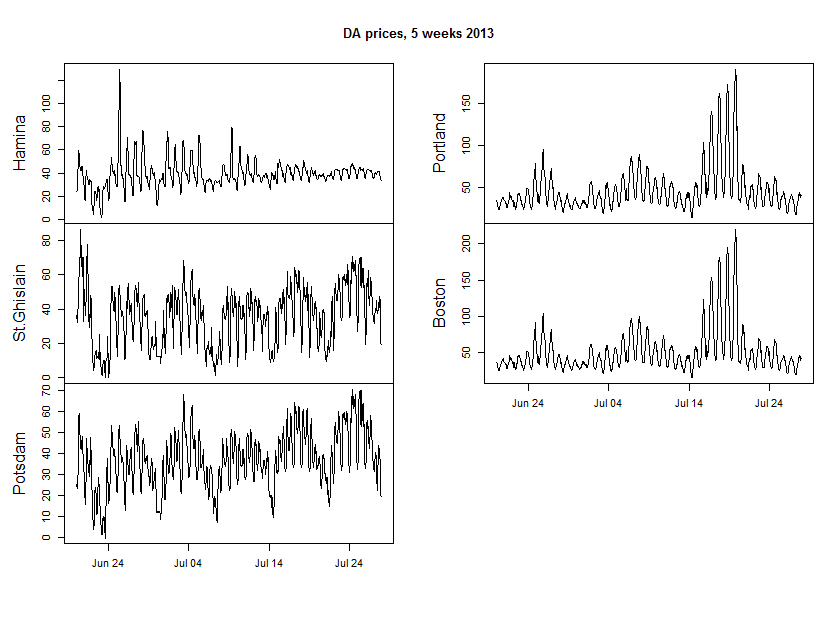
\includegraphics[width=1.0\textwidth]{figures/evaluation_and_results/da_sim_2013_5weeks.png}
	\caption{Day ahead energy prices over 5 weeks in 2013, in \$ per MWh}
	\label{fig:da_sim_2013_5weeks}
\end{figure}

The simulation has been run based on this dataset and previously defined cloud parameters. 
The following parameters have been set specifically for this simulation (Table \ref{tab:da_summer_cloud_parameters}). 


\begin{table}[htbp]
\centering
\begin{tabular}[\textwidth]{ll}
\toprule
	Cloud metric & Value  \\
\midrule
	number of servers & 500 \\
	number of servers per location & 100 \\
	number of virtual machines & 5000\\
\bottomrule
\end{tabular}
\caption{Cloud parameters for simulation scenario DA Summer}
\label{tab:da_summer_cloud_parameters}
\end{table}

The set of servers is distributed to locations such that each location is assigned to the same number of servers. Thus the number of servers has been chosen to accommodate the need for equal distribution regarding the number of locations. 


In this case the average utilization based on the calculation of Equation \ref{eq:average_utilization} would result in 15.7\%. 
Thus the cloud (number of servers, number of VMs) has been defined such that a sufficient amount of servers are available for VMs at each point in time and a reasonable value of cloud utilization is reached. 


Figure \ref{fig:DA_Summer_power_vs_cost} shows the results for normalized power vs cost for each scheduler. 
It can be noted that this shows very similar behavior to the results of the \textit{best utility function} in Section \ref{ssec:best_utility_function}. However in this simulation the BCU\_MF scheduler shows the least resulting costs relative to the baseline scheduler. This indicates a good performance of the utility function based on energy price forecasts which could outperform all other schedulers in terms of resulting costs. 

Figure \ref{fig:DA_Summer_total_cost} confirms these findings by displaying the total resulting costs for this simulation scenario. 
In this scenario no penalty costs due to migration downtimes have been resulted from any scheduler which attributes to high utility weights regarding SLA penalty and cost metrics. 

The resulting cloud metrics are depicted in Figure \ref{fig:DA_Summer_cloud_metrics}. This graph is similar to the cloud metrics of the best utility function with further reduced number of migrations of the BCU\_MF scheduler relative to the BCU\_M scheduler. Also total costs could be reduced due to less migration costs and less total cloud costs which is caused by a reduction of total power consumption. 

\begin{figure}[tbp]
	\centering
		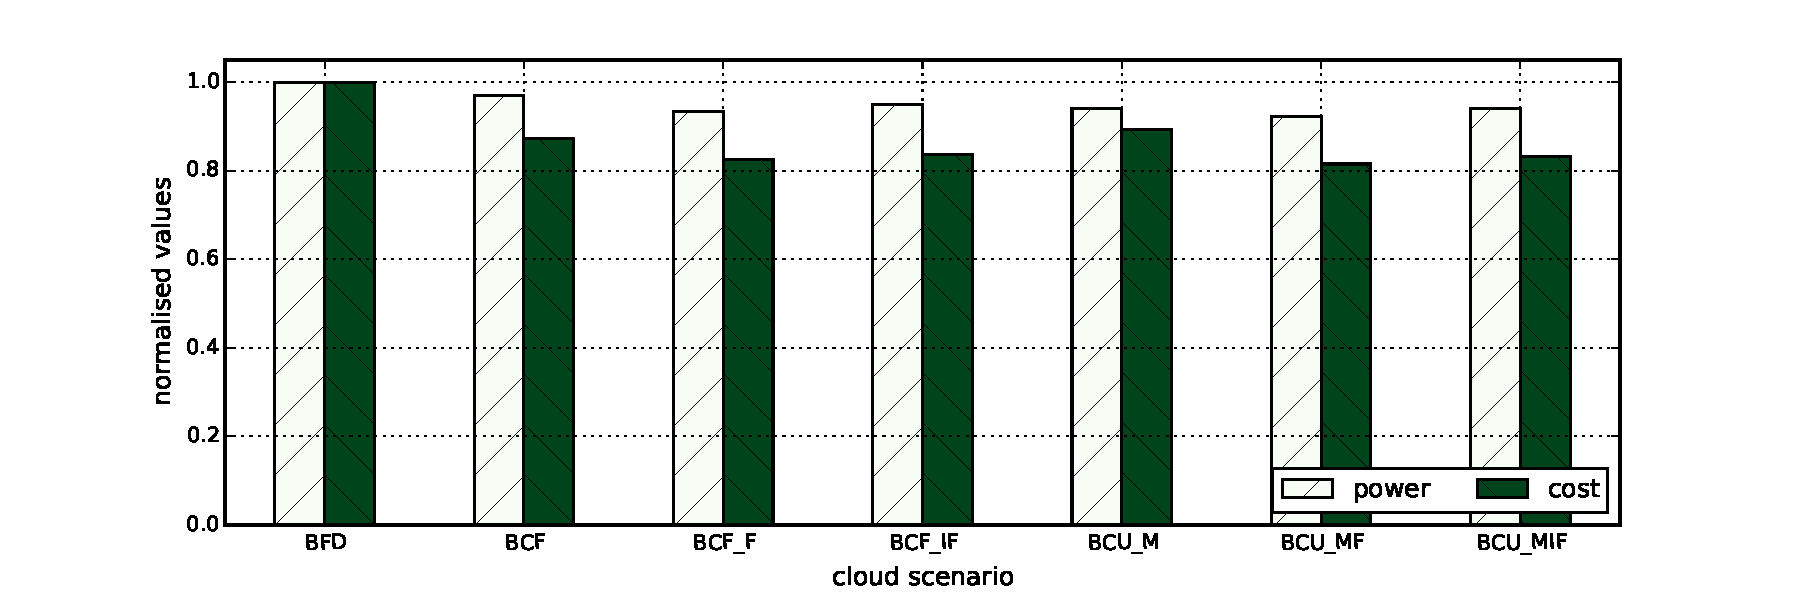
\includegraphics[width=1.00\textwidth]{figures/evaluation_and_results/DA_Summer_power_vs_cost.pdf}
	\caption{Normalized power and costs for DA Summer simulation scenario}
	\label{fig:DA_Summer_power_vs_cost}
\end{figure}

\begin{figure}[htbp]
	\centering
	\vspace*{-0.2in}
		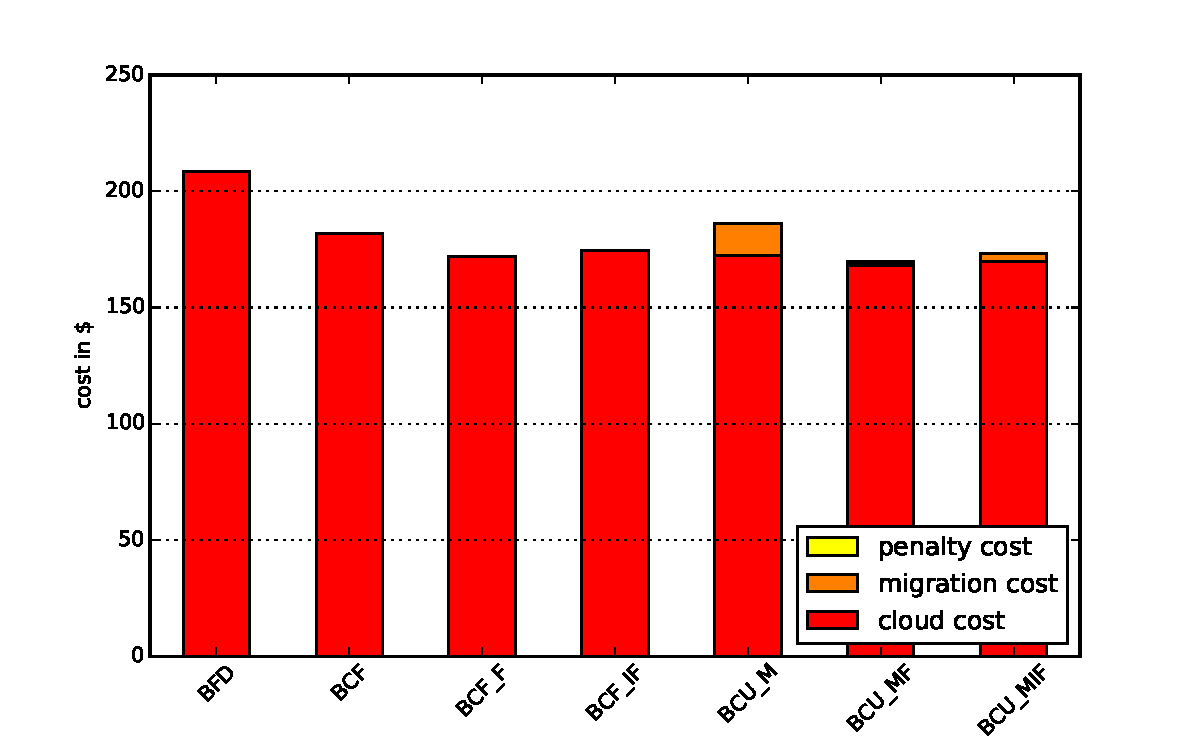
\includegraphics[width=0.7\textwidth]{figures/evaluation_and_results/DA_Summer_total_cost.pdf}
	\caption{Total resulting costs for DA Summer simulation scenario}
	\label{fig:DA_Summer_total_cost}
\end{figure}

\begin{figure}[bp]
	\centering
	\vspace*{-0.2in}
	\hspace*{-1.6in}
		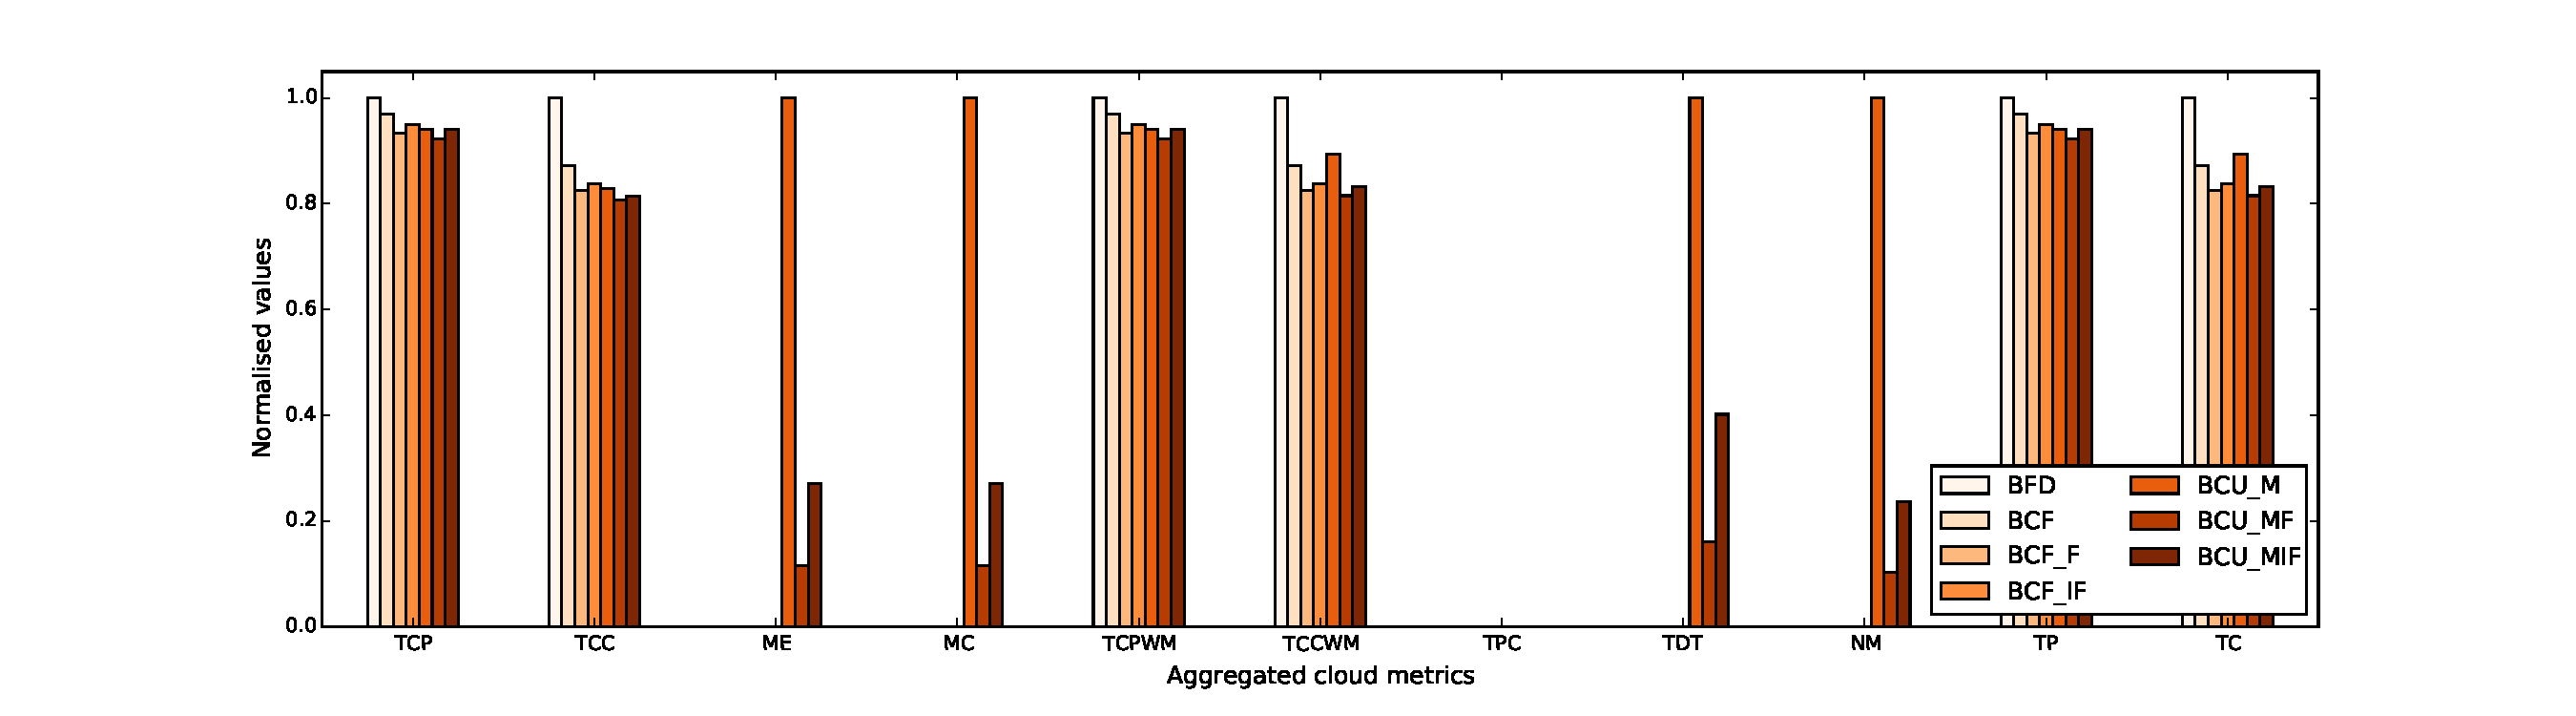
\includegraphics[width=1.50\textwidth]{figures/evaluation_and_results/DA_Summer_cloud_metrics.pdf}
	\caption{Cloud metrics resulting from the DA Summer simulation scenario}
	\label{fig:DA_Summer_cloud_metrics}
\end{figure}




\subsection{Simulation scenario DA Spring} \label{ssec:simulation_scenario_da_spring}

This simulation scenario is based on a total of 4 months of day ahead energy price data which should prove the validity of the schedulers based on an extended simulation time period. 

Figure \ref{fig:da_sim_2013_4months} shows the underlying dataset on which this simulation is based. 
Different time series show very different behavior in energy price variations. For example, Portland and Boston exhibit an increase in energy price levels of up to a factor of 10 during the period from January to March compared to prices after this period. Energy prices for Hamina on the contrary show a much more stable mean with just one significant spike at the beginning of March. This should result in a challenging scenario in terms of accurate forecast calculations for each location. 



\begin{figure}[htbp]
	\centering
		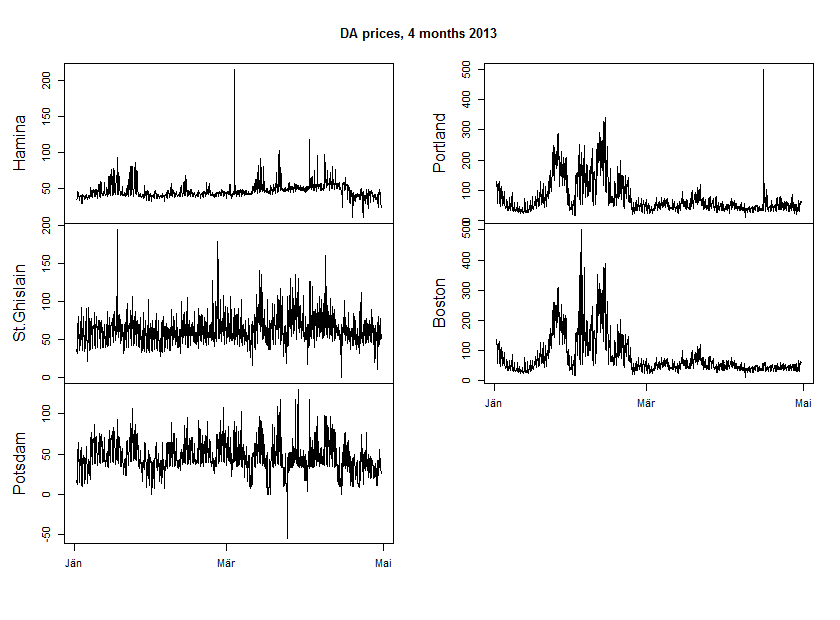
\includegraphics[width=1.0\textwidth]{figures/evaluation_and_results/da_sim_2013_4months.png}
	\caption{Day ahead energy prices over 4 months in 2013, in \$ per MWh}
	\label{fig:da_sim_2013_4months}
\end{figure}

Simulation specific parameters have been set according to Table \ref{tab:da_spring_cloud_parameters}. Thus the number of servers and servers per location has been defined analogously to the DA Summer simulation scenario but the number of virtual machines has been adjusted to accommodate the extended simulation time period. This results in an average utilization (VMs per server and point in time) of 14.9\% across the simulation time period. 

\begin{table}[htbp]
\centering
\begin{tabular}[\textwidth]{ll}
\toprule
	Cloud metric & Value  \\
\midrule
	number of servers & 500 \\
	number of servers per location & 100 \\
	number of virtual machines & 15000\\
\bottomrule
\end{tabular}
\caption{Cloud parameters for simulation scenario DA Spring}
\label{tab:da_spring_cloud_parameters}
\end{table}

From the results in Figure \ref{fig:DA_Spring_power_vs_cost} it is clearly visible that substantial cost savings have been achieved in this scenario compared to the BFD baseline scheduler. Even though the energy price dataset has not been optimal for applying forecasting methods the BCU\_MF scheduler which triggers migrations based on forecasts again results in the largest cost savings. Surprisingly the scheduler BCU\_MIF which is based on ideal forecasts is outperformed by the BCU\_MF scheduler which is based on actual forecasts generated for this dataset. This phenomenon can be attributed to the fact that the BCU\_MIF scheduler is highly impacted by occurring price spikes which may result in a higher number of migrations and thus resulting costs. 

\begin{figure}[htbp]
	\centering
		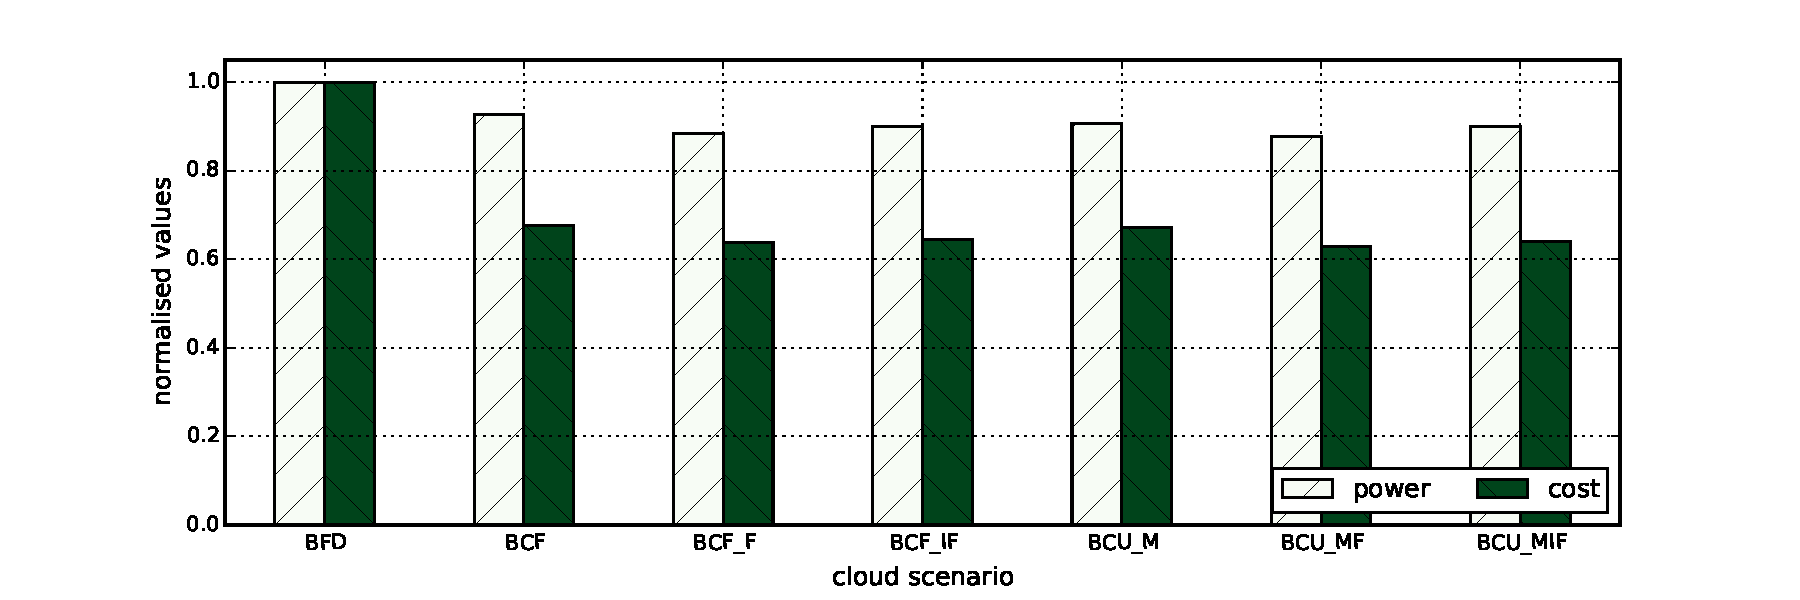
\includegraphics[width=1.00\textwidth]{figures/evaluation_and_results/DA_Spring_power_vs_cost.pdf}
	\caption{Normalized power and costs for DA Spring simulation scenario}
	\label{fig:DA_Spring_power_vs_cost}
\end{figure}

This is also emphasized by the total cost chart in Figure \ref{fig:DA_Spring_total_cost}. Due to a fewer number of migrations and different scheduling decisions the BCU\_MF scheduler results in less cloud costs attributed to less resulting cloud power. It can also be observed that the migration cost have been reduced to a negligible but still existing fraction of the total costs except for the BCU\_M scheduler. Therefore the cost difference between the BCU schedulers is caused due to different scheduling decisions and server consolidation resulting in different power and cost levels.

The graph showing cloud metrics confirms the statements made above (Figure \ref{fig:DA_Spring_cloud_metrics}). Total cloud power as well as total cloud costs could be significantly reduced compared to the BFD scheduler. The number of migrations and therefore migration costs could be greatly reduced as well for BCU\_MF and BCU\_MIF schedulers. The difference in total costs between the BCF and BCU schedulers is small but still significant. Interestingly the BCF\_F scheduler which is based on real forecasts outperforms both BCF and BCF\_IF schedulers in the same manner as it has been explained for BCU schedulers above. 

Therefore the BCU\_MF scheduler provides the best results for this simulation scenario similar to the DA Summer simulation.  

\begin{figure}[htbp]
	\centering
		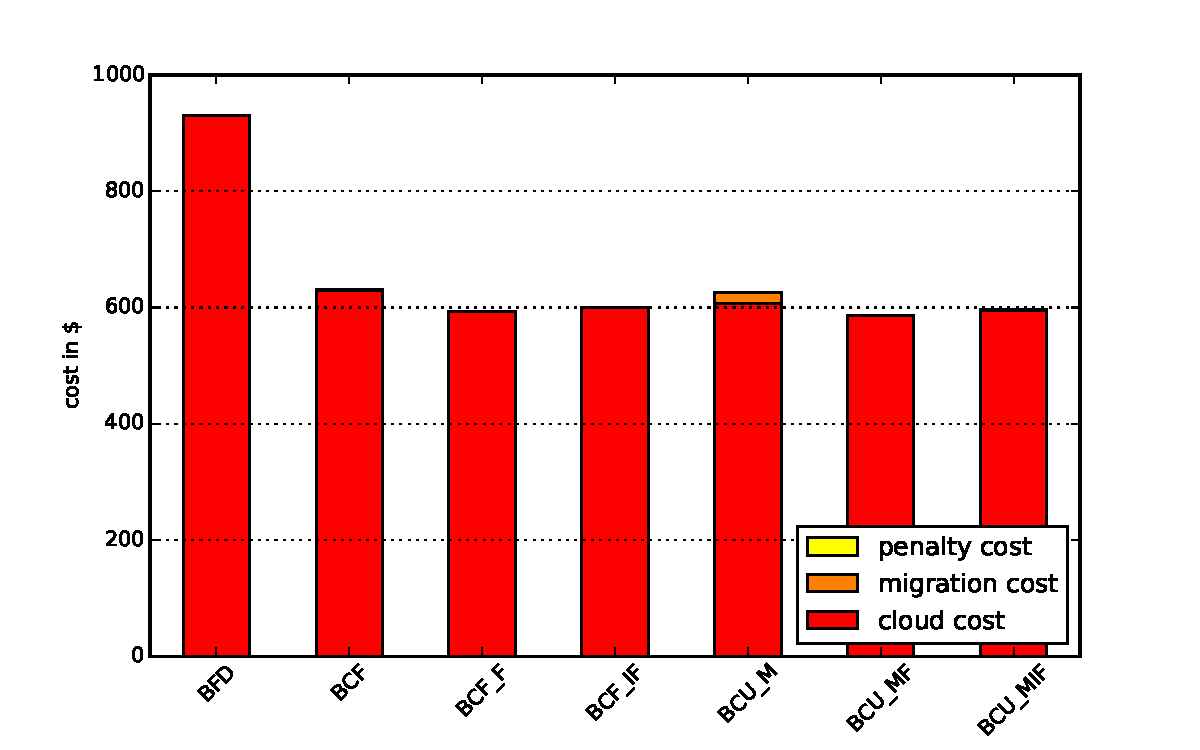
\includegraphics[width=0.7\textwidth]{figures/evaluation_and_results/DA_Spring_total_cost.pdf}
	\caption{Total resulting costs for DA Spring simulation scenario}
	\label{fig:DA_Spring_total_cost}
\end{figure}

\begin{figure}[htbp]
	\centering
	\hspace*{-1.2in}
		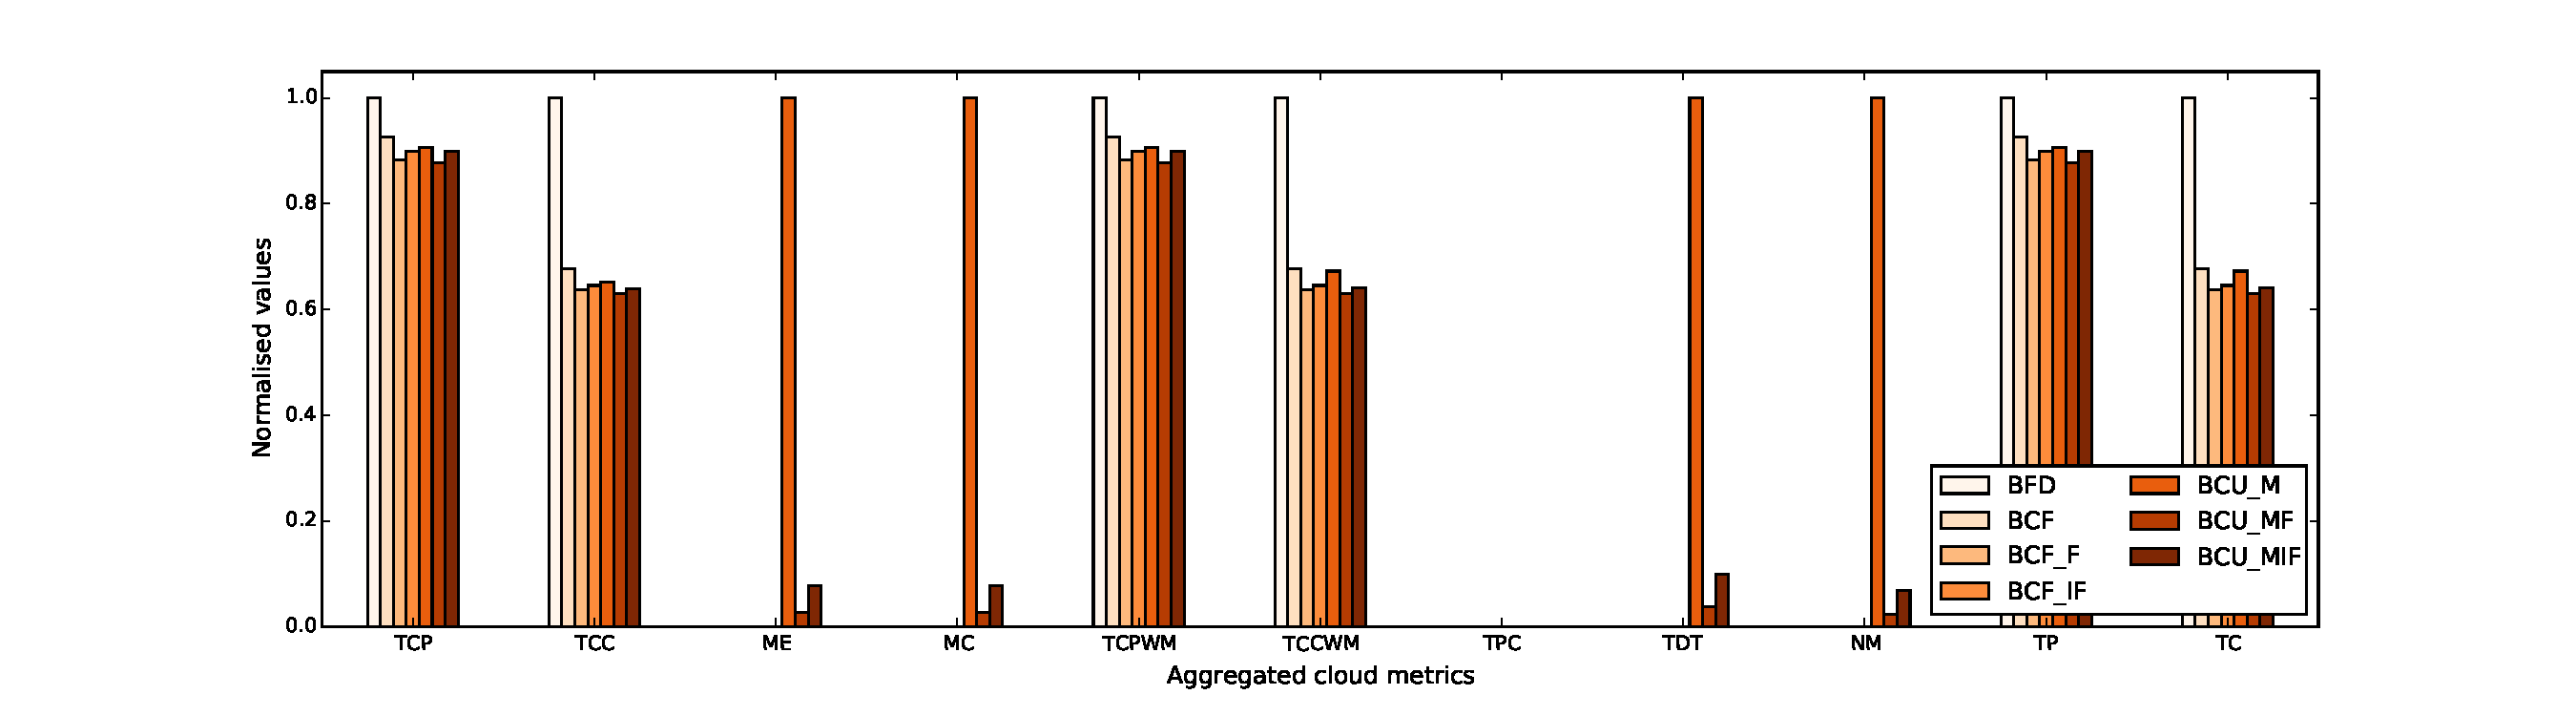
\includegraphics[width=1.50\textwidth]{figures/evaluation_and_results/DA_Spring_cloud_metrics.pdf}
	\caption{Cloud metrics resulting from the DA Spring simulation scenario}
	\label{fig:DA_Spring_cloud_metrics}
\end{figure}




\subsection{Simulation scenario RT Summer} \label{ssec:simulation_scenario_rt_summer}

This simulation scenario is again based on 5 weeks on energy price data however prices are retrieved from real time markets defined in Section \ref{sec:definition_of_simulation_scenarios}. 


Figure \ref{fig:rt_sim_2013_5weeks} shows the corresponding dataset for this simulation. Similar to the 5 week day ahead dataset it shows obvious daily and weekly seasonality with substantial increase in price levels beginning in mid of July. What is interesting to note is that all locations show similar price behavior over the whole simulation time period. This can be attributed to the fact that most of the locations are bound to the same energy market (PJM) and thus exhibit comparable patterns. Despite the locations Boston and Portland being associated with a different energy market (ISO New England) they show very similar patterns compared to the PJM locations. 

\begin{figure}[htbp]
	\centering
		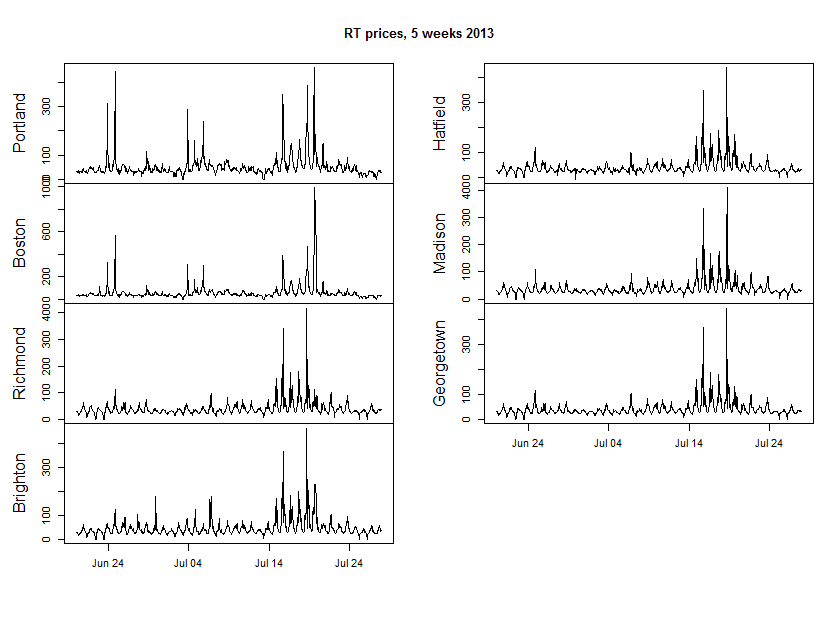
\includegraphics[width=1.00\textwidth]{figures/evaluation_and_results/rt_sim_2013_5weeks.png}
	\caption{Real time energy prices over 5 weeks in 2013, in \$ per MWh}
	\label{fig:rt_sim_2013_5weeks}
\end{figure}

The parameters applicable to this scenario are shown in Table \ref{tab:rt_summer_cloud_parameters}. The number of servers and virtual machines has been adjusted to fit the greater number of locations in this scenario. The resulting average utilization according to Equation \ref{eq:average_utilization} would be 15.7\% which is equal to the utilization of the DA Summer simulation. 

\begin{table}[htbp]
\centering
\begin{tabular}[\textwidth]{ll}
\toprule
	Cloud metric & Value  \\
\midrule
	number of servers & 700 \\
	number of servers per location & 100 \\
	number of virtual machines & 7000\\
\bottomrule
\end{tabular}
\caption{Cloud parameters for simulation scenario RT Summer}
\label{tab:rt_summer_cloud_parameters}
\end{table}

The normalized cost chart depicted in Figure \ref{fig:RT_Summer_power_vs_cost} shows slightly different patterns than the simulation scenarios presented for day ahead energy prices. In particular the schedulers exhibiting ideal forecasts (BCF\_IF and BCU\_MIF) provide the best results and the most cost reductions. This may be attributed to the fact that the real time price dataset for this simulation does not exhibit as many ``outliers'' or price spikes as the dataset associated with the DA Summer simulation over the same time period. Thus in this case the accurate ideal forecasts are not triggering too many unnecessary migrations and VMs do not need to be rescheduled as often leading to less power consumption and costs. 

\begin{figure}[htbp]
	\centering
		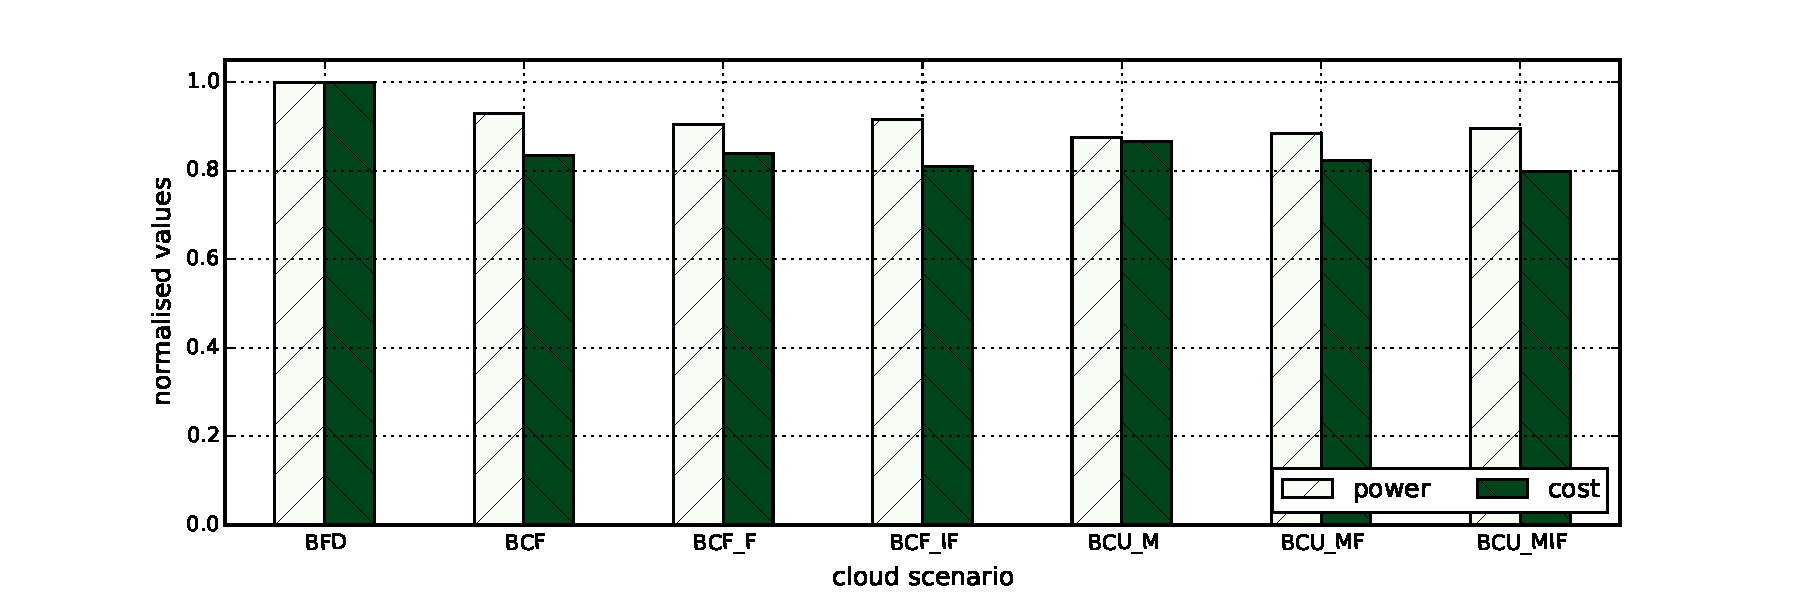
\includegraphics[width=1.00\textwidth]{figures/evaluation_and_results/RT_Summer_power_vs_cost.pdf}
	\caption{Normalized power and costs for RT Summer simulation scenario}
	\label{fig:RT_Summer_power_vs_cost}
\end{figure}

The same findings can be derived from the total cost chart in Figure \ref{fig:RT_Summer_power_vs_cost}. The BCU\_MIF scheduler results in slightly more migrations compared to the BCU\_MF scheduler but results in lower cost due to better utilization of the energy price differences for different locations. When comparing the BCU and BCF schedulers of the same type the former provide better performance than the latter in terms of cost reductions. Therefore it can be deduced that the utility functions operated at the BCU schedulers is well calibrated and provide reasonable results. 

The cloud metrics in Figure \ref{fig:RT_Summer_cloud_metrics} provide a detailed view on the results of the different metrics. Despite the increased power consumption caused by the BCU\_MIF scheduler it results in less total costs due to its ability to consider all occurring price differences. 
It also results in significantly more VM downtimes than the BCU\_MF scheduler however accumulated downtimes for individual VMs do not reach the penalty threshold. Therefore increased cost reductions come at the price of increased downtimes which are however not considered significant. 

\begin{figure}[htbp]
	\centering
		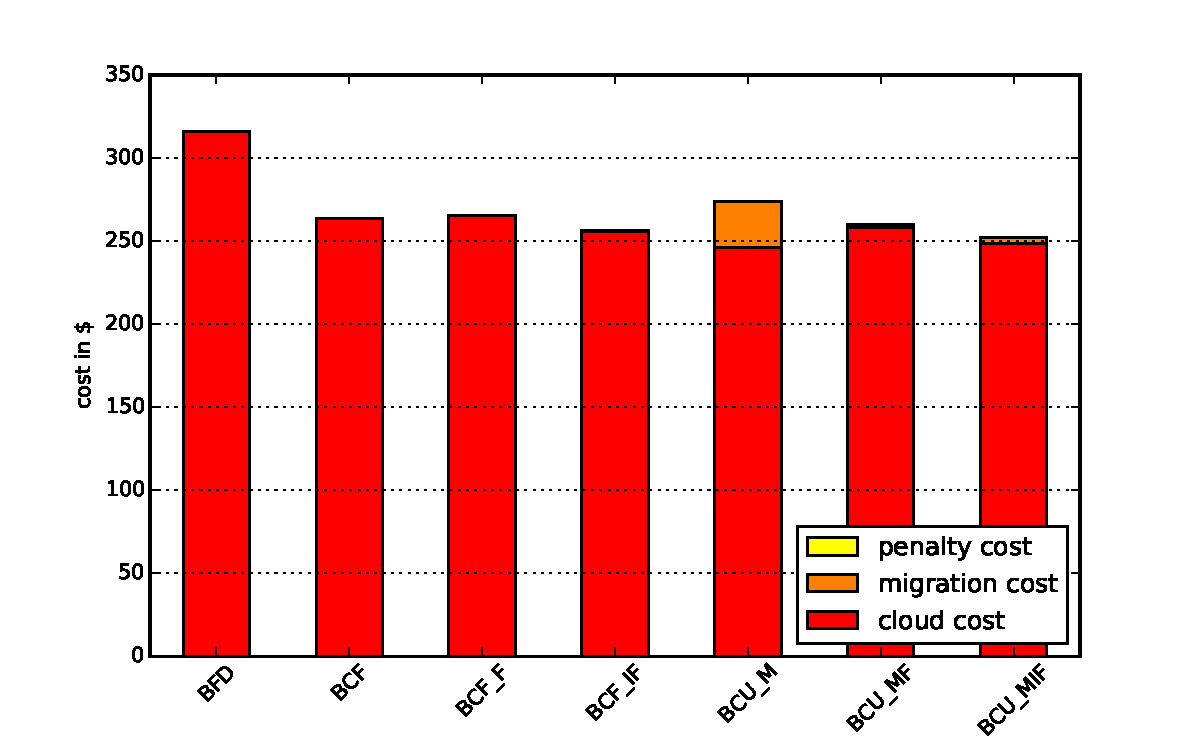
\includegraphics[width=0.7\textwidth]{figures/evaluation_and_results/RT_Summer_total_cost.pdf}
	\caption{Total resulting costs for RT Summer simulation scenario}
	\label{fig:RT_Summer_total_cost}
\end{figure}

\begin{figure}[htbp]
	\centering
	\hspace*{-1.6in}
		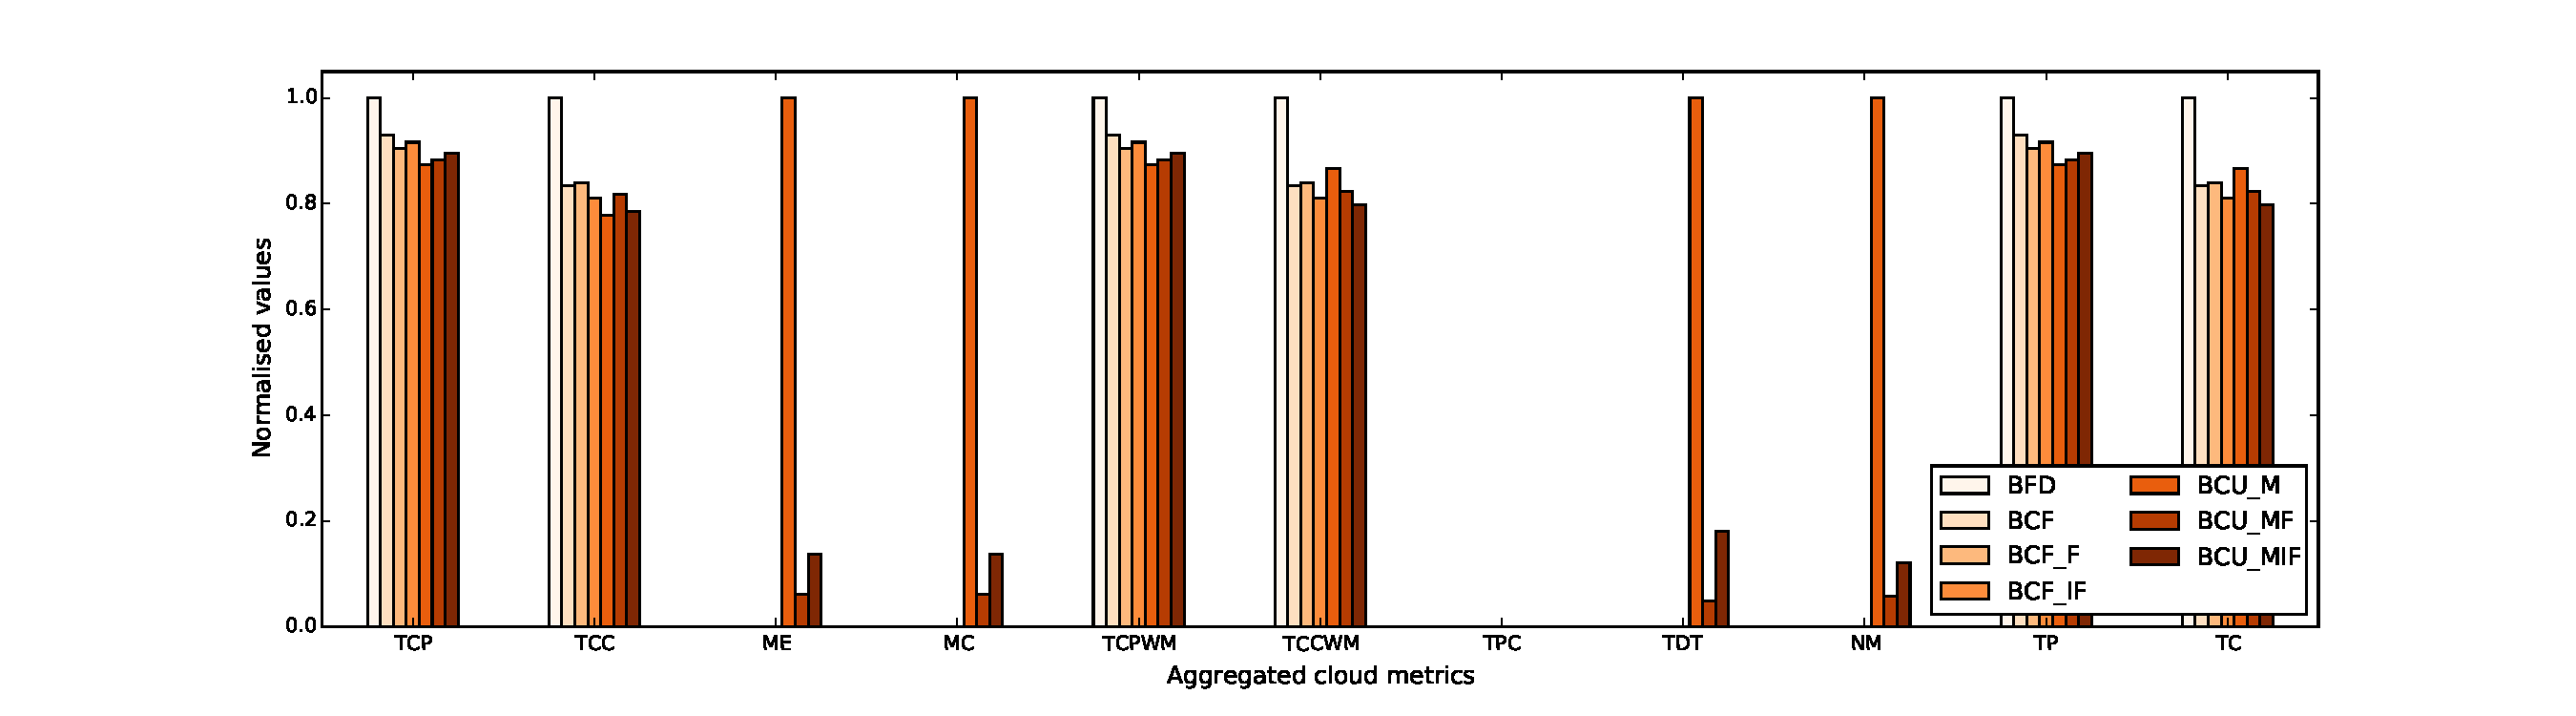
\includegraphics[width=1.50\textwidth]{figures/evaluation_and_results/RT_Summer_cloud_metrics.pdf}
	\caption{Cloud metrics resulting from the RT Summer simulation scenario}
	\label{fig:RT_Summer_cloud_metrics}
\end{figure}



\subsection{Simulation scenario RT Spring} \label{ssec:simulation_scenario_rt_spring}

The final simulation scenario is based on 4 months of real time energy prices. Analogously to the day ahead simulation DA Spring it exhibits the same time period but operates on a different dataset. The dataset associated with this simulation is outlined in Figure \ref{fig:rt_sim_2013_4months}. 

\begin{figure}[htbp]
	\centering
		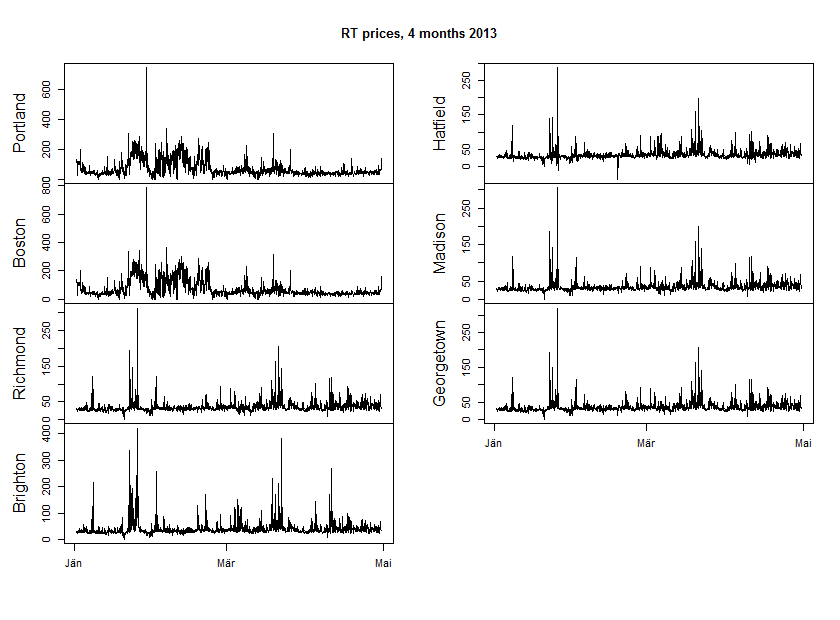
\includegraphics[width=1.00\textwidth]{figures/evaluation_and_results/rt_sim_2013_4months.png}
	\caption{Real time energy prices over 4 months in 2013, in \$ per MWh}
	\label{fig:rt_sim_2013_4months}
\end{figure}

Comparable to the dataset of the RT Summer simulation the locations belonging to the same energy market (see Section \ref{sec:definition_of_simulation_scenarios}) show very similar patterns over time. The PJM market locations experience a significant price spike at the end of January with another substantial increase in price levels in mid of March. The patterns may be similar but not identical, therefore it may still be sensible to migrate between locations of the PJM market. The locations Boston and Portland show similar patterns as their day ahead counterparts (see Section \ref{ssec:simulation_scenario_da_spring}). Thus a significant increase in price levels and variation can be observed from mid of January to mid of February in the graph which may result in less accurate forecasts. 

The cloud parameters specific to this simulation are depicted in Table \ref{tab:da_spring_cloud_parameters}. The relation of number of VMs to number of servers has been set the same as for the DA Spring simulation for a comparable distribution of VMs to servers. Therefore the average cloud utilization for this simulation scenario is 14.9\% which is the same as for the DA Spring simulation. 

\begin{table}[htbp]
\centering
\begin{tabular}[\textwidth]{ll}
\toprule
	Cloud metric & Value  \\
\midrule
	number of servers & 700 \\
	number of servers per location & 100 \\
	number of virtual machines & 21000\\
\bottomrule
\end{tabular}
\caption{Cloud parameters for simulation scenario DA Spring}
\label{tab:da_spring_cloud_parameters}
\end{table}

The normalized power and cost graph shows different results from the RT Summer simulation (Section \ref{ssec:simulation_scenario_rt_summer}). In this scenario the schedulers operating on real forecasts provide the best results in contrast to the schedulers based on ideal forecasts in the RT Summer simulation. After the investigations in the previous sections it can be stated that this behavior can be deduced with high probability from the characteristics of the energy price dataset. 
As energy prices tend to be more volatile in this scenario the schedulers based on real forecasts show an advantage of averaging extreme price values. In the previous simulation the price volatility has not been as high therefore the ideal forecasts exhibited an advantage. 


\begin{figure}[htbp]
	\centering
		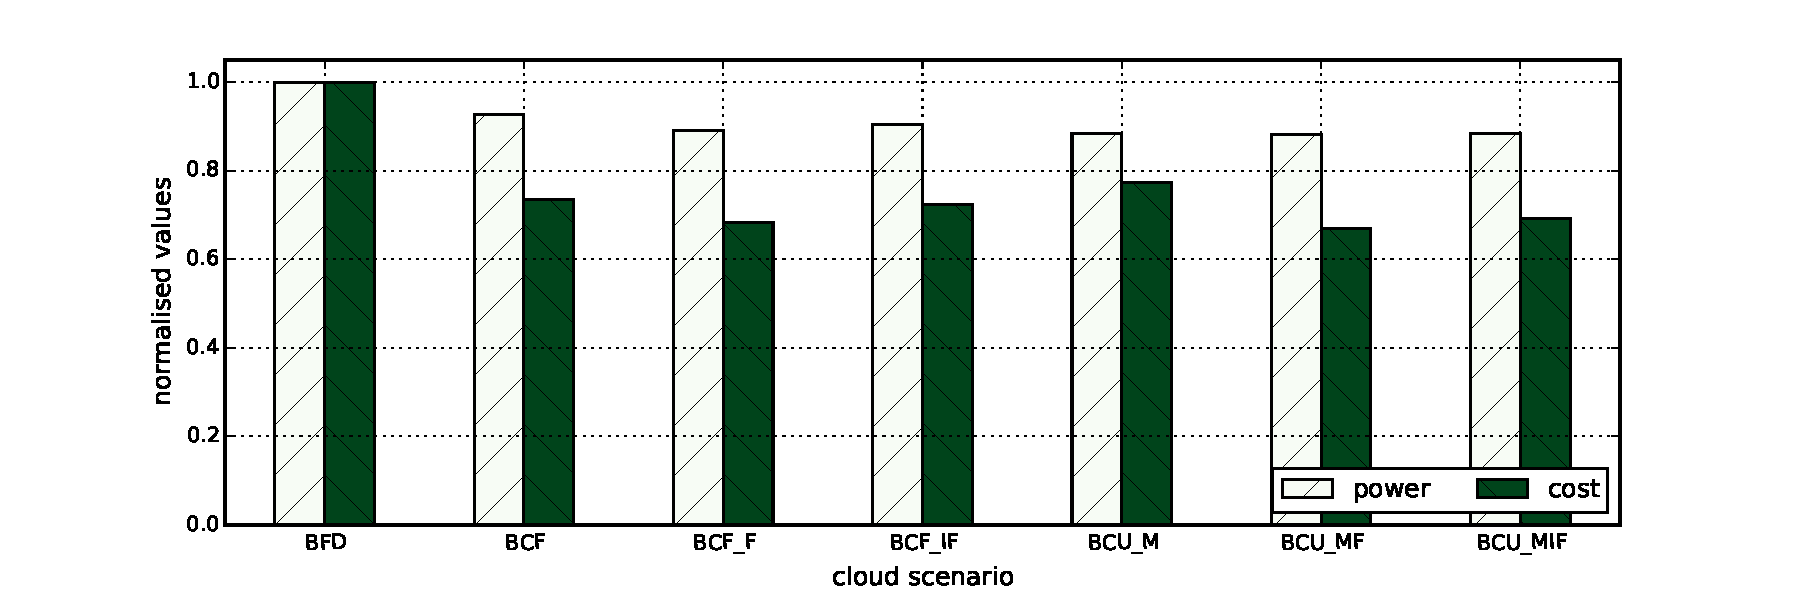
\includegraphics[width=1.00\textwidth]{figures/evaluation_and_results/RT_Spring_power_vs_cost.pdf}
	\caption{Normalized power and costs for RT Spring simulation scenario}
	\label{fig:RT_Spring_power_vs_cost}
\end{figure}

The total cost graph emphasizes these observations (Figure \ref{fig:RT_Spring_total_cost}). Compared to the DA Spring simulation (Section \ref{ssec:simulation_scenario_da_spring}) total costs show higher values for both cloud and migration costs. This can be attributed to the higher number of locations in this simulation which result in increased energy costs over the same simulation time period. 
As shown above the schedulers based on actual forecasts achieve the best results (BCF\_F, BCU\_MF). Thus the ``real'' forecast scheduler is suitable to be applied over a longer period of time with energy prices exhibiting high volatility. 

The resulting cloud metrics are depicted in Figure \ref{fig:RT_Spring_cloud_metrics}. Substantial power and cost reductions are clearly visible for total power and cost metrics. The BCU\_MF scheduler provides the best results with lowest energy costs and power consumption. In addition it experiences the least number of downtimes from all schedulers that include migrations (BCU\_M, BCU\_MF, BCU\_MIF). Therefore together with the findings earlier in this section it can be concluded that the BCU\_MF scheduler provides superior results for highly volatile energy price time series. 

\begin{figure}[htbp]
	\centering
		\includegraphics[width=0.7\textwidth]{figures/evaluation_and_results/RT_Spring_total_cost.pdf}
	\caption{Total resulting costs for RT Spring simulation scenario}
	\label{fig:RT_Spring_total_cost}
\end{figure}

\begin{figure}[htbp]
	\centering
	\hspace*{-1.2in}
		\includegraphics[width=1.50\textwidth]{figures/evaluation_and_results/RT_Spring_cloud_metrics.pdf}
	\caption{Cloud metrics resulting from the RT Spring simulation scenario}
	\label{fig:RT_Spring_cloud_metrics}
\end{figure}





\subsection{Utilization evaluation}

In order to better investigate the results presented in the previous sections the actual price time series vs their utilization levels have been investigated. Thus for each simulation scenario and each scheduler the cloud utilization has been printed together with the energy prices and corresponding forecasts. The results for the simulation RT Summer and the BCU\_MF scheduler are shown in Figure \ref{fig:RT_Summer_scenario_6}.

In this graph all locations are listed with each location showing a top and bottom graph. The top graph of each location shows the energy price time series over the simulation time period as a green line and the corresponding forecasts as overlay as a red line. The bottom graph shows the changes of utilization over time for each location, that is the actual total server utilization per time. 

Results show substantial variations in utilization levels over the simulation time period. The change in utilization is triggered by the actual forecasts (red line) as the BCU\_MF scheduler evaluates the utility function based on real forecasts. This can be observed when investigating the location Richmond and its utilization levels. 

The utilization at this location shows a drop in utilization levels beginning from 16th of July due to increased forecasted prices at this time. Thus the load is moved to other locations exhibiting a reduced energy price at this point in time. The same behavior can be observed for the locations Hatfield and Georgetown where utilization drops around the same time. 

In contrast location Madison shows more stable utilization levels with still a trough around the same time where drops in utilization have been observed for other locations. Locations Boston and Portland have not experienced high utilization on average as the effort of moving resources to these locations is higher due to lower bandwidth connections (see Table \ref{tab:real_time_bandwidth_mappings}). 

However around the same time at mid of July Portland experiences a substantial increase in load which is shifted from other locations. The reason might be the small drop in energy price forecasts at this location on the 16th of July as well as a lower forecasted average price over the next hours. 

Utilization levels increase up to 50 percent at times (see location Portland) but average utilization per location varies from very low values to about 25 percent depending on the scenario. As the weights of the utility function (see Section \ref{ssec:best_utility_function}) have been set to high values for SLA penalties and cost reductions but to a low value for data center load the primary reason for VM migration are to mitigate SLA penalties due to VM downtimes and enhance cost reductions based on cheaper energy prices. Load balancing has not been considered as important metric in the presented simulations. 

The resulting graphs for all locations, all simulations and all schedulers have been placed in the Appendix for reference (\ref{sec:app_result_simulation_graphs}). The BFD scheduler in the RT summer simulation does not consider any energy price changes in its scheduling decisions and thus load is distributed uniformly over all locations (see \ref{fig:app_RT_Summer_scenario_1}). This results in similar utilization at all locations where average utilization levels for this scheduler evolve around 8 to 10 percent. 

\begin{figure}[htbp]
	\centering
	\vspace*{-0.6in}
	\hspace*{-1.4in}
		\includegraphics[width=1.60\textwidth]{figures/evaluation_and_results/RT_Summer_scenario_6.pdf}
	\vspace*{-1.0in}
	\caption{Energy prices, energy price forecasts and utilization levels per location for simulation RT Summer and scheduler BCU\_MF}
	\label{fig:RT_Summer_scenario_6}
\end{figure}

The BCU\_M scheduler only considers current energy prices for migrations which leads to very high number of migrations and high volatility in the utilization (see \ref{fig:app_RT_Spring_scenario_5}). For the RT Spring simulation this is best visible for location Portland which exhibits a very high number of ``spikes'' in utilization. Thus due to high variations in energy prices a high number of migrations have been performed. 

When comparing the behavior of the schedulers based on actual and ideal forecasts (BCU\_MF, BCU\_MIF) it can be observed that the BCU\_MIF scheduler exhibits a higher number of migrations (higher volatility of utilization) than the BCU\_MF scheduler (see \ref{fig:app_DA_Spring_scenario_6} and \ref{fig:app_DA_Spring_scenario_7} for locations Hamina and Potsdam). This confirms the fact described before that the BCU\_MIF scheduler is more sensitive to price changes and tends to trigger migrations more frequently. 

When observing simulation results for DA Summer for scheduler BCU\_MF (see \ref{fig:app_DA_Summer_scenario_6}) the relation of forecasts to actual energy prices can be seen more clearly. It seems that the forecasted energy prices ``lag behind'' the actual energy prices by a certain amount of time. Daily seasonality can be clearly spotted also in forecasted energy prices with similar patterns as they exist in actual energy prices, best visible for locations Portland and Boston. 

However for the real time price scenario shown in Figure \ref{fig:RT_Summer_scenario_6} it can be observed that the forecasts do not model the exact price time series but average out price spikes that may occur in the energy price time series. Therefore schedulers incorporating real forecasts in contrast to ideal forecasts can be seen as an advantage for highly volatile price series as they do not consider each price spike but model energy prices more closely to their mean. 
Thus ideal forecasts may even lead to sub-optimal scheduling decisions as results showed in DA Spring and RT Spring simulations (see linked Sections \ref{ssec:simulation_scenario_da_spring} and \ref{ssec:simulation_scenario_rt_spring}). 


\subsection{Simulation results}

The simulation scenarios discussed in the previous sections provide a clear hint for the most suitable scheduling algorithm for a given dataset. 
In case of datasets exhibiting mid to high range volatility the BCU\_MF scheduler results in lowest total costs whereas for datasets with more stable volatility the BCU\_MIF scheduler provides best results. 

%The different graphs provide an insight into energy price and forecasting behavior

From the investigations 

\begin{table}[htbp]
\centering
\begin{tabular}[\textwidth]{ll}
\toprule
	Simulation Name & Utilization  \\
\midrule
	DA Summer & 15.7 \\
	DA Spring & 14.9 \\
	RT Summer & 15.7 \\
	RT Spring & 14.9 \\
\bottomrule
\end{tabular}
\caption{Resulting cloud utilization per simulation scenario}
\label{tab:cloud_utilization_per_simulation_scenario}
\end{table}

The formula to calculate the average utilization values in Table \ref{tab:cloud_utilization_per_simulation_scenario} is defined in Equation \ref{eq:average_utilization}.
As the relation of number of VMs to number of servers has been set the same for DA and RT simulations the resulting average cloud utilization are the same for each of the Summer and Spring simulations. 

\subsection{Total costs}


\begin{table}[ht]
\centering
\begin{tabular}{lrrrrrrr}
\toprule
{} &     BFD &     BCF &   BCF\_F &  BCF\_IF &   BCU\_M &  BCU\_MF &  BCU\_MIF \\
\midrule
DA Summer &  208.36 &  181.72 &  171.85 &  174.53 &  186.19 &  \textbf{169.86} &   173.29 \\
RT Summer &  315.96 &  263.32 &  265.21 &  256.08 &  273.87 &  259.98 &   \textbf{252.09} \\
DA Spring &  930.41 &  630.13 &  592.83 &  600.42 &  625.62 &  \textbf{585.97} &   595.81 \\
RT Spring &  966.04 &  710.59 &  659.92 &  699.13 &  747.06 &  \textbf{647.57} &   668.35 \\
\bottomrule
\end{tabular}
\caption{Total costs for different scenarios (in \$)}
\end{table}

\begin{table}[ht]
\centering
\begin{tabular}{lrrrrrrr}
\toprule
{} &  BFD &    BCF &  BCF\_F &  BCF\_IF &  BCU\_M &  BCU\_MF &  BCU\_MIF \\
\midrule
DA Summer &    0 &  12.79 &  17.52 &   16.24 &  10.64 &   \textbf{18.48} &    16.83 \\
RT Summer &    0 &  16.66 &  16.06 &   18.95 &  13.32 &   17.72 &    \textbf{20.21} \\
DA Spring &    0 &  32.27 &  36.28 &   35.47 &  32.76 &   \textbf{37.02} &    35.96 \\
RT Spring &    0 &  26.44 &  31.69 &   27.63 &  22.67 &   \textbf{32.97} &    30.82 \\
\bottomrule
\end{tabular}
\caption{Normalized total cost reductions for different scenarios (in \%)}
\end{table}







%%%%%%%%%%%%%%%%%%%%%%%%%%%%%%%%%%%%%%%%%
\chapter{Conclusion and Future Work}
\label{ch:conclusion}
%%%%%%%%%%%%%%%%%%%%%%%%%%%%%%%%%%%%%%%%%






ARIMA models showed reasonably good performance, in many cases they showed the best results compared to other evaluated models in this work. 







In \cite{de2013study} it is shown that the cost of optimal assignment is further reduced by increasing the number of locations with data centers assigned to different energy markets and/or by increasing the variability of energy prices. 


\section{Benefits and limitations}



...

As Qureshi et al.~pointed out in \cite{qureshi2009cutting} most companies would need to renegotiate their energy contracts in order to utilize the proposed approach. Companies renting space in co-location facilities usually pay a fixed price for energy rather than directly taking part in the price offers of wholesale markets. 

Demand response programs are a way of further decreasing energy costs as consumers agree on a reduced price in exchange for a reduced load when it is requested by the grid operator\cite{albadi2008summary}. This is certainly interesting for energy elastic distributed systems that are able to shift load to other locations dynamically. 






\section{Future Work}


Forecasting models may be improved, or different models may be investigated based on electricity price data. 

Dynamic Regression (DR) and Transfer function (TF) models have been shown to provide a significantly better performance than ARIMA models \cite{aggarwal2009electricity,weron2005forecasting}. This may be due to the additional regressor variables that are considered in multivariate models (DR and TF) in contrast to models based on a single univariate time series (ARIMA). 

In general multivariate models seem to provide better results than univariate models as they are able to include more information into the model generation process \cite{weron2005forecasting}. 



\appendix

%%%%%%%%%%%%%%%%%%%%%%%%%%%%%%%%%%%%%%%%%
\chapter{Forecast Evaluation Results}
\label{ch:appendix_forecast_results}
%%%%%%%%%%%%%%%%%%%%%%%%%%%%%%%%%%%%%%%%%



\section{Result tables}




%  Generated from R function getRMSEResults: Get results from forecast simulation 
% -----------------------
% Get results from forecast simulation for the given location
% over a time range of 3 years, generate models in intervals of 1 week
% with 2,3 and 4 weeks of trainings data periods
% 5 locations are available from the forecast simulation (Application server):
%  1) Hamina, locationId 1, DA
%  2) St.Ghislain, locationId 2, DA
%  3) Portland, locationId 4, RT
%  4) Richmond, locationId 6, RT
%  5) Hatfield, locationId 8, RT



\subsection{Forecast evaluation results for Hamina (DA)}


%> getRMSEResults(1)
% latex table generated in R 3.1.1 by xtable 1.8-2 package
% Mon Mar 07 21:56:45 2016
\begin{table}[ht]
\centering
\begin{tabular}{rrrrrrrrrrr}
  \hline
 & 1h & 3h & 6h & 12h & 18h & 24h & 36h & 48h & 96h & 168h \\ 
  \hline
mean & 14.55 & 14.55 & 14.55 & 14.55 & 14.55 & 14.55 & 14.55 & 14.55 & 14.55 & 14.55 \\ 
  ses & 2.13 & 3.54 & 5.06 & 15.83 & 16.38 & 14.98 & 14.97 & 14.64 & 15.13 & 13.30 \\ 
  holts & 1.91 & 3.36 & 9.48 & 30.83 & 38.85 & 44.08 & 58.79 & 74.25 & 137.44 & 228.66 \\ 
  holtwinters & 3.20 & 7.11 & 13.10 & 26.07 & 36.13 & 45.85 & 65.02 & 85.30 & 166.43 & 288.31 \\ 
  arima & 2.11 & 3.06 & 4.63 & 13.68 & 13.92 & 12.69 & 12.88 & 12.62 & 13.69 & 12.97 \\ 
  tbats & 2.15 & 2.89 & 4.35 & 10.63 & 10.85 & 10.00 & 10.16 & 9.90 & 10.66 & 10.30 \\ 
   \hline
\end{tabular}
\caption{Aggregated values for RMSE for a trainings period of 2 weeks}
\end{table}
% latex table generated in R 3.1.1 by xtable 1.8-2 package
% Mon Mar 07 21:56:45 2016
\begin{table}[ht]
\centering
\begin{tabular}{rrrrrrrrrrr}
  \hline
 & 1h & 3h & 6h & 12h & 18h & 24h & 36h & 48h & 96h & 168h \\ 
  \hline
mean & 14.78 & 14.78 & 14.78 & 14.78 & 14.78 & 14.78 & 14.78 & 14.78 & 14.78 & 14.78 \\ 
  ses & 2.14 & 3.56 & 5.06 & 15.84 & 16.38 & 14.98 & 14.97 & 14.63 & 15.14 & 13.31 \\ 
  holts & 1.91 & 3.38 & 9.51 & 30.88 & 38.90 & 44.15 & 58.90 & 74.39 & 137.77 & 229.23 \\ 
  holtwinters & 3.08 & 7.08 & 13.15 & 27.16 & 37.14 & 46.56 & 65.62 & 85.74 & 166.63 & 288.04 \\ 
  arima & 2.06 & 2.88 & 4.31 & 12.94 & 13.08 & 11.89 & 11.97 & 11.66 & 12.71 & 11.79 \\ 
  tbats & 2.15 & 3.05 & 4.73 & 11.27 & 11.43 & 10.55 & 10.60 & 10.35 & 11.07 & 10.68 \\ 
   \hline
\end{tabular}
\caption{Aggregated values for RMSE for a trainings period of 3 weeks}
\end{table}
% latex table generated in R 3.1.1 by xtable 1.8-2 package
% Mon Mar 07 21:56:45 2016
\begin{table}[ht]
\centering
\begin{tabular}{rrrrrrrrrrr}
  \hline
 & 1h & 3h & 6h & 12h & 18h & 24h & 36h & 48h & 96h & 168h \\ 
  \hline
mean & 14.99 & 14.99 & 14.99 & 14.99 & 14.99 & 14.99 & 14.99 & 14.99 & 14.99 & 14.99 \\ 
  ses & 2.13 & 3.57 & 5.06 & 15.84 & 16.38 & 14.97 & 14.96 & 14.61 & 15.13 & 13.30 \\ 
  holts & 1.89 & 3.37 & 9.53 & 31.00 & 39.07 & 44.34 & 59.18 & 74.75 & 138.54 & 230.59 \\ 
  holtwinters & 5.52 & 11.00 & 17.21 & 33.23 & 44.51 & 54.36 & 75.54 & 97.71 & 187.49 & 324.07 \\ 
  arima & 1.98 & 2.85 & 4.39 & 12.68 & 12.79 & 11.61 & 11.73 & 11.36 & 12.07 & 11.13 \\ 
  tbats & 2.18 & 3.08 & 4.64 & 10.99 & 11.19 & 10.32 & 10.46 & 10.21 & 10.94 & 10.40 \\ 
   \hline
\end{tabular}
\caption{Aggregated values for RMSE for a trainings period of 4 weeks}
\end{table}



\subsection{Results for St. Ghislain (DA)}

\begin{landscape}
%> getRMSEResults(2)
% latex table generated in R 3.1.1 by xtable 1.8-2 package
% Mon Mar 07 21:56:56 2016
\begin{table}[ht]
\centering
\begin{tabular}{rrrrrrrrrrr}
  \hline
 & 1h & 3h & 6h & 12h & 18h & 24h & 36h & 48h & 96h & 168h \\ 
  \hline
mean & 1.71E+01 & 1.71E+01 & 1.71E+01 & 1.71E+01 & 1.71E+01 & 1.71E+01 & 1.71E+01 & 1.71E+01 & 1.71E+01 & 1.71E+01 \\ 
  ses & 8.32E+00 & 1.14E+01 & 1.40E+01 & 1.66E+01 & 1.65E+01 & 1.71E+01 & 1.69E+01 & 1.71E+01 & 1.75E+01 & 1.71E+01 \\ 
  holts & 7.88E+00 & 1.13E+01 & 1.81E+01 & 4.52E+01 & 6.27E+01 & 8.08E+01 & 1.14E+02 & 1.49E+02 & 2.88E+02 & 4.94E+02 \\ 
  holtwinters & 1.08E+01 & 2.10E+01 & 3.42E+01 & 6.14E+01 & 8.68E+01 & 1.13E+02 & 1.64E+02 & 2.16E+02 & 4.24E+02 & 7.36E+02 \\ 
  arima & 6.86E+00 & 7.10E+00 & 7.82E+00 & 1.43E+01 & 1.54E+01 & 1.54E+01 & 1.56E+01 & 1.61E+01 & 1.78E+01 & 1.85E+01 \\ 
  tbats & 4.86E+49 & 1.05E+50 & 1.46E+50 & 1.45E+50 & 1.40E+50 & 1.39E+50 & 1.38E+50 & 1.37E+50 & 1.36E+50 & 1.35E+50 \\ 
   \hline
\end{tabular}
\end{table}
% latex table generated in R 3.1.1 by xtable 1.8-2 package
% Mon Mar 07 21:56:56 2016
\begin{table}[ht]
\centering
\begin{tabular}{rrrrrrrrrrr}
  \hline
 & 1h & 3h & 6h & 12h & 18h & 24h & 36h & 48h & 96h & 168h \\ 
  \hline
mean & 17.40 & 17.40 & 17.40 & 17.40 & 17.40 & 17.40 & 17.40 & 17.40 & 17.40 & 17.40 \\ 
  ses & 8.37 & 11.41 & 14.07 & 16.64 & 16.56 & 17.08 & 16.88 & 17.10 & 17.50 & 17.10 \\ 
  holts & 7.80 & 11.29 & 18.07 & 45.41 & 63.10 & 81.37 & 114.61 & 150.60 & 290.39 & 497.90 \\ 
  holtwinters & 10.42 & 18.66 & 31.72 & 61.43 & 86.38 & 114.50 & 167.20 & 220.67 & 434.85 & 756.26 \\ 
  arima & 6.72 & 6.61 & 7.07 & 13.92 & 15.02 & 14.98 & 15.26 & 15.66 & 17.05 & 17.12 \\ 
  tbats & 6.09 & 6.52 & 7.11 & 11.94 & 13.16 & 13.39 & 13.70 & 14.09 & 14.96 & 15.05 \\ 
   \hline
\end{tabular}
\end{table}
% latex table generated in R 3.1.1 by xtable 1.8-2 package
% Mon Mar 07 21:56:56 2016
\begin{table}[ht]
\centering
\begin{tabular}{rrrrrrrrrrr}
  \hline
 & 1h & 3h & 6h & 12h & 18h & 24h & 36h & 48h & 96h & 168h \\ 
  \hline
mean & 1.76E+01 & 1.76E+01 & 1.76E+01 & 1.76E+01 & 1.76E+01 & 1.76E+01 & 1.76E+01 & 1.76E+01 & 1.76E+01 & 1.76E+01 \\ 
  ses & 8.38E+00 & 1.15E+01 & 1.41E+01 & 1.67E+01 & 1.66E+01 & 1.71E+01 & 1.69E+01 & 1.71E+01 & 1.75E+01 & 1.71E+01 \\ 
  holts & 7.82E+00 & 1.13E+01 & 1.81E+01 & 4.51E+01 & 6.27E+01 & 8.07E+01 & 1.14E+02 & 1.49E+02 & 2.88E+02 & 4.94E+02 \\ 
  holtwinters & 9.68E+00 & 2.09E+01 & 3.43E+01 & 6.09E+01 & 8.59E+01 & 1.12E+02 & 1.64E+02 & 2.16E+02 & 4.24E+02 & 7.35E+02 \\ 
  arima & 6.82E+00 & 6.91E+00 & 7.56E+00 & 1.41E+01 & 1.50E+01 & 1.49E+01 & 1.51E+01 & 1.54E+01 & 1.65E+01 & 1.64E+01 \\ 
  tbats & 2.53E+35 & 2.17E+36 & 3.83E+36 & 2.88E+36 & 3.16E+36 & 2.83E+36 & 2.73E+36 & 2.63E+36 & 2.36E+36 & 2.07E+36 \\ 
   \hline
\end{tabular}
\end{table}


\subsection{Results for Portland (RT)}

%> getRMSEResults(4)
% latex table generated in R 3.1.1 by xtable 1.8-2 package
% Mon Mar 07 21:57:07 2016
\begin{table}[ht]
\centering
\begin{tabular}{rrrrrrrrrrr}
  \hline
 & 1h & 3h & 6h & 12h & 18h & 24h & 36h & 48h & 96h & 168h \\ 
  \hline
mean & 2.42E+01 & 2.42E+01 & 2.42E+01 & 2.42E+01 & 2.42E+01 & 2.42E+01 & 2.42E+01 & 2.42E+01 & 2.42E+01 & 2.42E+01 \\ 
  ses & 7.92E+00 & 1.07E+01 & 1.29E+01 & 2.11E+01 & 2.76E+01 & 2.84E+01 & 2.83E+01 & 3.03E+01 & 3.40E+01 & 3.49E+01 \\ 
  holts & 1.67E+01 & 2.63E+01 & 4.25E+01 & 8.45E+01 & 1.20E+02 & 1.50E+02 & 2.10E+02 & 2.74E+02 & 5.28E+02 & 9.06E+02 \\ 
  holtwinters & 2.20E+01 & 5.02E+01 & 8.13E+01 & 1.39E+02 & 1.96E+02 & 2.50E+02 & 3.58E+02 & 4.71E+02 & 9.18E+02 & 1.59E+03 \\ 
  arima & 9.61E+00 & 1.36E+01 & 1.59E+01 & 2.00E+01 & 2.59E+01 & 2.68E+01 & 2.71E+01 & 2.93E+01 & 3.43E+01 & 3.77E+01 \\ 
  tbats & 9.61E+16 & 5.92E+16 & 6.82E+16 & 7.15E+16 & 6.03E+16 & 5.48E+16 & 4.56E+16 & 3.97E+16 & 2.81E+16 & 2.13E+16 \\ 
   \hline
\end{tabular}
\end{table}
% latex table generated in R 3.1.1 by xtable 1.8-2 package
% Mon Mar 07 21:57:07 2016
\begin{table}[ht]
\centering
\begin{tabular}{rrrrrrrrrrr}
  \hline
 & 1h & 3h & 6h & 12h & 18h & 24h & 36h & 48h & 96h & 168h \\ 
  \hline
mean & 2.41E+01 & 2.41E+01 & 2.41E+01 & 2.41E+01 & 2.41E+01 & 2.41E+01 & 2.41E+01 & 2.41E+01 & 2.41E+01 & 2.41E+01 \\ 
  ses & 7.96E+00 & 1.06E+01 & 1.29E+01 & 2.10E+01 & 2.76E+01 & 2.83E+01 & 2.82E+01 & 3.03E+01 & 3.39E+01 & 3.49E+01 \\ 
  holts & 1.68E+01 & 2.66E+01 & 4.30E+01 & 8.54E+01 & 1.21E+02 & 1.52E+02 & 2.13E+02 & 2.78E+02 & 5.35E+02 & 9.19E+02 \\ 
  holtwinters & 2.27E+01 & 5.37E+01 & 1.08E+02 & 2.19E+02 & 3.12E+02 & 4.13E+02 & 6.06E+02 & 8.02E+02 & 1.58E+03 & 2.75E+03 \\ 
  arima & 9.42E+00 & 1.30E+01 & 1.58E+01 & 1.92E+01 & 2.45E+01 & 2.52E+01 & 2.52E+01 & 2.69E+01 & 3.07E+01 & 3.26E+01 \\ 
  tbats & 2.24E+18 & 2.61E+18 & 2.31E+18 & 1.98E+18 & 1.76E+18 & 1.58E+18 & 1.33E+18 & 1.16E+18 & 8.24E+17 & 6.23E+17 \\ 
   \hline
\end{tabular}
\end{table}
% latex table generated in R 3.1.1 by xtable 1.8-2 package
% Mon Mar 07 21:57:07 2016
\begin{table}[ht]
\centering
\begin{tabular}{rrrrrrrrrrr}
  \hline
 & 1h & 3h & 6h & 12h & 18h & 24h & 36h & 48h & 96h & 168h \\ 
  \hline
mean & 2.47E+01 & 2.47E+01 & 2.47E+01 & 2.47E+01 & 2.47E+01 & 2.47E+01 & 2.47E+01 & 2.47E+01 & 2.47E+01 & 2.47E+01 \\ 
  ses & 7.70E+00 & 1.03E+01 & 1.26E+01 & 2.08E+01 & 2.74E+01 & 2.81E+01 & 2.80E+01 & 3.01E+01 & 3.37E+01 & 3.47E+01 \\ 
  holts & 1.65E+01 & 2.71E+01 & 4.60E+01 & 9.40E+01 & 1.35E+02 & 1.69E+02 & 2.39E+02 & 3.13E+02 & 6.04E+02 & 1.04E+03 \\ 
  holtwinters & 1.86E+01 & 4.37E+01 & 7.95E+01 & 1.40E+02 & 2.05E+02 & 2.66E+02 & 3.86E+02 & 5.09E+02 & 9.99E+02 & 1.73E+03 \\ 
  arima & 8.63E+00 & 1.25E+01 & 1.54E+01 & 1.88E+01 & 2.42E+01 & 2.49E+01 & 2.49E+01 & 2.67E+01 & 3.05E+01 & 3.25E+01 \\ 
  tbats & 3.55E+31 & 3.00E+32 & 2.59E+32 & 2.40E+32 & 2.34E+32 & 2.31E+32 & 2.27E+32 & 2.25E+32 & 2.18E+32 & 2.11E+32 \\ 
   \hline
\end{tabular}
\end{table}

\subsection{Results for Richmond (RT)}

%> getRMSEResults(6)
% latex table generated in R 3.1.1 by xtable 1.8-2 package
% Mon Mar 07 21:57:13 2016
\begin{table}[ht]
\centering
\begin{tabular}{rrrrrrrrrrr}
  \hline
 & 1h & 3h & 6h & 12h & 18h & 24h & 36h & 48h & 96h & 168h \\ 
  \hline
mean & 1.45E+01 & 1.45E+01 & 1.45E+01 & 1.45E+01 & 1.45E+01 & 1.45E+01 & 1.45E+01 & 1.45E+01 & 1.45E+01 & 1.45E+01 \\ 
  ses & 4.62E+00 & 6.13E+00 & 6.20E+00 & 1.28E+01 & 1.66E+01 & 1.89E+01 & 2.11E+01 & 2.27E+01 & 2.24E+01 & 2.03E+01 \\ 
  holts & 5.48E+00 & 1.12E+01 & 2.17E+01 & 5.24E+01 & 7.60E+01 & 9.72E+01 & 1.37E+02 & 1.78E+02 & 3.35E+02 & 5.71E+02 \\ 
  holtwinters & 1.34E+01 & 3.32E+01 & 5.85E+01 & 1.06E+02 & 1.50E+02 & 1.96E+02 & 2.84E+02 & 3.74E+02 & 7.34E+02 & 1.27E+03 \\ 
  arima & 4.23E+00 & 6.09E+00 & 7.15E+00 & 1.33E+01 & 1.61E+01 & 1.83E+01 & 2.07E+01 & 2.20E+01 & 2.20E+01 & 2.05E+01 \\ 
  tbats & 4.88E+13 & 3.37E+13 & 6.17E+13 & 1.04E+14 & 1.01E+14 & 8.86E+13 & 8.59E+13 & 8.22E+13 & 7.72E+13 & 7.47E+13 \\ 
   \hline
\end{tabular}
\end{table}
% latex table generated in R 3.1.1 by xtable 1.8-2 package
% Mon Mar 07 21:57:13 2016
\begin{table}[ht]
\centering
\begin{tabular}{rrrrrrrrrrr}
  \hline
 & 1h & 3h & 6h & 12h & 18h & 24h & 36h & 48h & 96h & 168h \\ 
  \hline
mean & 1.45E+01 & 1.45E+01 & 1.45E+01 & 1.45E+01 & 1.45E+01 & 1.45E+01 & 1.45E+01 & 1.45E+01 & 1.45E+01 & 1.45E+01 \\ 
  ses & 4.70E+00 & 6.19E+00 & 6.26E+00 & 1.29E+01 & 1.66E+01 & 1.90E+01 & 2.11E+01 & 2.28E+01 & 2.25E+01 & 2.03E+01 \\ 
  holts & 5.74E+00 & 1.15E+01 & 2.21E+01 & 5.24E+01 & 7.58E+01 & 9.68E+01 & 1.36E+02 & 1.77E+02 & 3.33E+02 & 5.67E+02 \\ 
  holtwinters & 1.38E+01 & 3.46E+01 & 5.68E+01 & 1.03E+02 & 1.46E+02 & 1.93E+02 & 2.83E+02 & 3.71E+02 & 7.26E+02 & 1.26E+03 \\ 
  arima & 3.78E+00 & 5.49E+00 & 6.12E+00 & 1.20E+01 & 1.50E+01 & 1.73E+01 & 1.99E+01 & 2.13E+01 & 2.11E+01 & 1.94E+01 \\ 
  tbats & 2.88E+00 & 4.41E+00 & 4.90E+00 & 1.14E+01 & 1.46E+01 & 1.69E+01 & 1.93E+01 & 2.09E+01 & 2.06E+01 & 1.88E+01 \\ 
   \hline
\end{tabular}
\end{table}
% latex table generated in R 3.1.1 by xtable 1.8-2 package
% Mon Mar 07 21:57:13 2016
\begin{table}[ht]
\centering
\begin{tabular}{rrrrrrrrrrr}
  \hline
 & 1h & 3h & 6h & 12h & 18h & 24h & 36h & 48h & 96h & 168h \\ 
  \hline
mean & 1.44E+01 & 1.44E+01 & 1.44E+01 & 1.44E+01 & 1.44E+01 & 1.44E+01 & 1.44E+01 & 1.44E+01 & 1.44E+01 & 1.44E+01 \\ 
  ses & 4.73E+00 & 6.25E+00 & 6.29E+00 & 1.29E+01 & 1.66E+01 & 1.90E+01 & 2.12E+01 & 2.29E+01 & 2.26E+01 & 2.04E+01 \\ 
  holts & 5.70E+00 & 1.14E+01 & 2.20E+01 & 5.24E+01 & 7.60E+01 & 9.72E+01 & 1.37E+02 & 1.78E+02 & 3.35E+02 & 5.72E+02 \\ 
  holtwinters & 1.43E+01 & 3.78E+01 & 6.41E+01 & 1.16E+02 & 1.66E+02 & 2.19E+02 & 3.20E+02 & 4.18E+02 & 8.13E+02 & 1.41E+03 \\ 
  arima & 3.70E+00 & 5.44E+00 & 6.04E+00 & 1.21E+01 & 1.51E+01 & 1.73E+01 & 1.99E+01 & 2.12E+01 & 2.10E+01 & 1.94E+01 \\ 
  tbats & 5.83E+55 & 2.82E+99 & 1.36E+109 & 9.65E+108 & 7.88E+108 & 6.82E+108 & 5.57E+108 & 4.82E+108 & 3.41E+108 & 2.58E+108 \\ 
   \hline
\end{tabular}
\end{table}

\end{landscape}





%%%% aggregated results %%%%


%
%%s <- 1
%%> data <- forecastAggregateByWeek(simPrefix[s], simPostFix)
%%> printXTable(data)
%% latex table generated in R 3.1.1 by xtable 1.8-2 package
%% Mon Mar 07 23:02:44 2016
%\begin{table}[ht]
%\centering
%\begin{tabular}{rrrrrrr}
  %\hline
 %& mean & ses & holts & holtwinters & arima & tbats \\ 
  %\hline
%2 weeks & 14.55 & 11.60 & 62.76 & 73.65 & 10.23 & 8.19 \\ 
  %3 weeks & 14.78 & 11.60 & 62.90 & 74.02 & 9.53 & 8.59 \\ 
  %4 weeks & 14.99 & 11.60 & 63.23 & 85.06 & 9.26 & 8.44 \\ 
   %\hline
%\end{tabular}
%\end{table}
%%> s <- 2
%%> data <- forecastAggregateByWeek(simPrefix[s], simPostFix)
%%> printXTable(data)
%% latex table generated in R 3.1.1 by xtable 1.8-2 package
%% Mon Mar 07 23:03:25 2016
%\begin{table}[ht]
%\centering
%\begin{tabular}{rrrrrrr}
  %\hline
 %& mean & ses & holts & holtwinters & arima & tbats \\ 
  %\hline
%2 weeks & 1.71E+01 & 1.52E+01 & 1.27E+02 & 1.87E+02 & 1.35E+01 & 1.27E+50 \\ 
  %3 weeks & 1.74E+01 & 1.53E+01 & 1.28E+02 & 1.90E+02 & 1.29E+01 & 1.16E+01 \\ 
  %4 weeks & 1.76E+01 & 1.53E+01 & 1.27E+02 & 1.86E+02 & 1.29E+01 & 2.49E+36 \\ 
   %\hline
%\end{tabular}
%\end{table}
%%> s <- 3
%%> data <- forecastAggregateByWeek(simPrefix[s], simPostFix)
%%> printXTable(data)
%% latex table generated in R 3.1.1 by xtable 1.8-2 package
%% Mon Mar 07 23:04:19 2016
%\begin{table}[ht]
%\centering
%\begin{tabular}{rrrrrrr}
  %\hline
 %& mean & ses & holts & holtwinters & arima & tbats \\ 
  %\hline
%2 weeks & 2.42E+01 & 2.36E+01 & 2.36E+02 & 4.07E+02 & 2.40E+01 & 5.45E+16 \\ 
  %3 weeks & 2.41E+01 & 2.36E+01 & 2.39E+02 & 6.87E+02 & 2.23E+01 & 1.64E+18 \\ 
  %4 weeks & 2.47E+01 & 2.33E+01 & 2.68E+02 & 4.38E+02 & 2.19E+01 & 2.18E+32 \\ 
   %\hline
%\end{tabular}
%\end{table}
%%> s <- 4
%%> data <- forecastAggregateByWeek(simPrefix[s], simPostFix)
%%> printXTable(data)
%% latex table generated in R 3.1.1 by xtable 1.8-2 package
%% Mon Mar 07 23:04:33 2016
%\begin{table}[ht]
%\centering
%\begin{tabular}{rrrrrrr}
  %\hline
 %& mean & ses & holts & holtwinters & arima & tbats \\ 
  %\hline
%2 weeks & 1.45E+01 & 1.52E+01 & 1.49E+02 & 3.22E+02 & 1.50E+01 & 7.57E+13 \\ 
  %3 weeks & 1.45E+01 & 1.52E+01 & 1.48E+02 & 3.19E+02 & 1.41E+01 & 1.35E+01 \\ 
  %4 weeks & 1.44E+01 & 1.53E+01 & 1.49E+02 & 3.58E+02 & 1.41E+01 & 5.44E+108 \\ 
   %\hline
%\end{tabular}
%\end{table}
%
%
%
%%%% aggregated with real values %%%%
%
%
%% latex table generated in R 3.1.1 by xtable 1.8-2 package
%% Mon Mar 07 23:15:14 2016
%\begin{table}[ht]
%\centering
%\begin{tabular}{rrrrrrr}
  %\hline
 %& mean & ses & holts & holtwinters & arima & tbats \\ 
  %\hline
%2 weeks & 14.55 & 11.60 & 62.76 & 73.65 & 10.23 & 8.19 \\ 
  %3 weeks & 14.78 & 11.60 & 62.90 & 74.02 & 9.53 & 8.59 \\ 
  %4 weeks & 14.99 & 11.60 & 63.23 & 85.06 & 9.26 & 8.44 \\ 
   %\hline
%\end{tabular}
%\end{table}
%% latex table generated in R 3.1.1 by xtable 1.8-2 package
%% Mon Mar 07 23:15:14 2016
%\begin{table}[ht]
%\centering
%\begin{tabular}{rrrrrrr}
  %\hline
 %& mean & ses & holts & holtwinters & arima & tbats \\ 
  %\hline
%2 weeks & 17.07 & 15.23 & 127.13 & 186.82 & 13.49 & 127083769482826530120880468026666642684682684202440.00 \\ 
  %3 weeks & 17.40 & 15.27 & 128.05 & 190.21 & 12.94 & 11.60 \\ 
  %4 weeks & 17.59 & 15.30 & 127.03 & 186.37 & 12.87 & 2489183418470472805280220406686824466.00 \\ 
   %\hline
%\end{tabular}
%\end{table}
%% latex table generated in R 3.1.1 by xtable 1.8-2 package
%% Mon Mar 07 23:15:14 2016
%\begin{table}[ht]
%\centering
%\begin{tabular}{rrrrrrr}
  %\hline
 %& mean & ses & holts & holtwinters & arima & tbats \\ 
  %\hline
%2 weeks & 24.22 & 23.61 & 235.84 & 407.06 & 24.03 & 54480307964830568.00 \\ 
  %3 weeks & 24.14 & 23.56 & 238.92 & 686.95 & 22.26 & 1641463958726746880.00 \\ 
  %4 weeks & 24.68 & 23.32 & 268.10 & 437.85 & 21.91 & 218087279314998705120640862002240.00 \\ 
   %\hline
%\end{tabular}
%\end{table}
%% latex table generated in R 3.1.1 by xtable 1.8-2 package
%% Mon Mar 07 23:15:14 2016
%\begin{table}[ht]
%\centering
%\begin{tabular}{rrrrrrr}
  %\hline
 %& mean & ses & holts & holtwinters & arima & tbats \\ 
  %\hline
%2 weeks & 14.47 & 15.17 & 148.54 & 322.41 & 15.03 & 75718511564550.16 \\ 
  %3 weeks & 14.46 & 15.23 & 147.77 & 318.61 & 14.14 & 13.46 \\ 
  %4 weeks & 14.42 & 15.29 & 148.67 & 357.82 & 14.11 & 5436976252839544085822686600406264624462846648628408864880264806208282628200002428820226822648622602228826246.00 \\ 
   %\hline
%\end{tabular}
%\end{table}




\section{Result graphs}





%%%%%%%%%%%%%%%%%%%%%%%%%%%%%%%%%%%%%%%%%
\chapter{Simulation Results}
\label{ch:appendix_simulation_results}
%%%%%%%%%%%%%%%%%%%%%%%%%%%%%%%%%%%%%%%%%



\section{Result tables} \label{sec:app_result_simulation_tables}



\subsection{Cloud metrics results}

\begin{table}[ht]
\centering
\begin{tabular}{lrrrrrrr}
\toprule
{} &       BFD &       BCU &     BCU\_F &    BCU\_IF &     BCU\_M &    BCU\_MF &   BCU\_MIF \\
\midrule
TCP   &  21501.23 &  19938.71 &  19173.33 &  19437.17 &  18978.17 &  18979.72 &  19016.16 \\
TCC   &    966.04 &    710.59 &    659.92 &    699.13 &    673.24 &    645.01 &    660.06 \\
ME    &      0.00 &      0.00 &      0.00 &      0.00 &     10.51 &      0.37 &      1.18 \\
MC    &      0.00 &      0.00 &      0.00 &      0.00 &     73.82 &      2.56 &      8.29 \\
TCPWM &  21501.23 &  19938.71 &  19173.33 &  19437.17 &  18988.68 &  18980.09 &  19017.34 \\
TCCWM &    966.04 &    710.59 &    659.92 &    699.13 &    747.06 &    647.57 &    668.35 \\
TPC   &      0.00 &      0.00 &      0.00 &      0.00 &      0.00 &      0.00 &      0.00 \\
TDT   &      0.00 &      0.00 &      0.00 &      0.00 &  24578.00 &    773.00 &   3787.00 \\
NM    &      0.00 &      0.00 &      0.00 &      0.00 &  14401.00 &    476.00 &   1398.00 \\
TP    &  21501.23 &  19938.71 &  19173.33 &  19437.17 &  18988.68 &  18980.09 &  19017.34 \\
TC    &    966.04 &    710.59 &    659.92 &    699.13 &    747.06 &    647.57 &    668.35 \\
\bottomrule
\end{tabular}
\caption{Cloud metrics for simulation "`RT Spring"'}
\end{table}


\begin{table}[ht]
\centering
\begin{tabular}{lrrrrrrr}
\toprule
{} &      BFD &      BCU &    BCU\_F &   BCU\_IF &    BCU\_M &   BCU\_MF &  BCU\_MIF \\
\midrule
TCP   &  6922.22 &  6435.57 &  6263.45 &  6343.36 &  6048.94 &  6113.84 &  6198.98 \\
TCC   &   315.96 &   263.32 &   265.21 &   256.08 &   245.97 &   258.30 &   248.28 \\
ME    &     0.00 &     0.00 &     0.00 &     0.00 &     3.97 &     0.24 &     0.54 \\
MC    &     0.00 &     0.00 &     0.00 &     0.00 &    27.90 &     1.69 &     3.81 \\
TCPWM &  6922.22 &  6435.57 &  6263.45 &  6343.36 &  6052.91 &  6114.08 &  6199.52 \\
TCCWM &   315.96 &   263.32 &   265.21 &   256.08 &   273.87 &   259.98 &   252.09 \\
TPC   &     0.00 &     0.00 &     0.00 &     0.00 &     0.00 &     0.00 &     0.00 \\
TDT   &     0.00 &     0.00 &     0.00 &     0.00 &  9575.00 &   461.00 &  1729.00 \\
NM    &     0.00 &     0.00 &     0.00 &     0.00 &  5580.00 &   319.00 &   671.00 \\
TP    &  6922.22 &  6435.57 &  6263.45 &  6343.36 &  6052.91 &  6114.08 &  6199.52 \\
TC    &   315.96 &   263.32 &   265.21 &   256.08 &   273.87 &   259.98 &   252.09 \\
\bottomrule
\end{tabular}
\caption{Cloud metrics for simulation "`RT Summer"'}
\end{table}


\begin{table}[ht]
\centering
\begin{tabular}{lrrrrrrr}
\toprule
{} &       BFD &       BCU &     BCU\_F &    BCU\_IF &     BCU\_M &    BCU\_MF &   BCU\_MIF \\
\midrule
TCP   &  15338.31 &  14211.48 &  13545.14 &  13789.94 &  13903.81 &  13462.65 &  13794.13 \\
TCC   &    930.41 &    630.13 &    592.83 &    600.42 &    606.20 &    585.45 &    594.32 \\
ME    &      0.00 &      0.00 &      0.00 &      0.00 &      2.76 &      0.07 &      0.21 \\
MC    &      0.00 &      0.00 &      0.00 &      0.00 &     19.42 &      0.53 &      1.49 \\
TCPWM &  15338.31 &  14211.48 &  13545.14 &  13789.94 &  13906.57 &  13462.72 &  13794.34 \\
TCCWM &    930.41 &    630.13 &    592.83 &    600.42 &    625.62 &    585.97 &    595.81 \\
TPC   &      0.00 &      0.00 &      0.00 &      0.00 &      0.00 &      0.00 &      0.00 \\
TDT   &      0.00 &      0.00 &      0.00 &      0.00 &  12728.00 &    482.00 &   1269.00 \\
NM    &      0.00 &      0.00 &      0.00 &      0.00 &   3332.00 &     75.00 &    228.00 \\
TP    &  15338.31 &  14211.48 &  13545.14 &  13789.94 &  13906.57 &  13462.72 &  13794.34 \\
TC    &    930.41 &    630.13 &    592.83 &    600.42 &    625.62 &    585.97 &    595.81 \\
\bottomrule
\end{tabular}
\caption{Cloud metrics for simulation "`DA Spring"'}
\end{table}


\begin{table}[ht]
\centering
\begin{tabular}{lrrrrrrr}
\toprule
{} &      BFD &      BCU &    BCU\_F &   BCU\_IF &    BCU\_M &   BCU\_MF &  BCU\_MIF \\
\midrule
TCP   &  4984.39 &  4830.12 &  4652.92 &  4731.71 &  4688.42 &  4597.72 &  4685.54 \\
TCC   &   208.36 &   181.72 &   171.85 &   174.53 &   172.50 &   168.28 &   169.60 \\
ME    &     0.00 &     0.00 &     0.00 &     0.00 &     1.95 &     0.22 &     0.53 \\
MC    &     0.00 &     0.00 &     0.00 &     0.00 &    13.69 &     1.58 &     3.70 \\
TCPWM &  4984.39 &  4830.12 &  4652.92 &  4731.71 &  4690.37 &  4597.95 &  4686.07 \\
TCCWM &   208.36 &   181.72 &   171.85 &   174.53 &   186.19 &   169.86 &   173.29 \\
TPC   &     0.00 &     0.00 &     0.00 &     0.00 &     0.00 &     0.00 &     0.00 \\
TDT   &     0.00 &     0.00 &     0.00 &     0.00 &  8716.00 &  1401.00 &  3499.00 \\
NM    &     0.00 &     0.00 &     0.00 &     0.00 &  2162.00 &   221.00 &   510.00 \\
TP    &  4984.39 &  4830.12 &  4652.92 &  4731.71 &  4690.37 &  4597.95 &  4686.07 \\
TC    &   208.36 &   181.72 &   171.85 &   174.53 &   186.19 &   169.86 &   173.29 \\
\bottomrule
\end{tabular}
\caption{Cloud metrics for simulation "`DA Summer"'}
\end{table}



\FloatBarrier
\section{Result graphs} \label{sec:app_result_simulation_graphs}


\subsection{Simulation results for DA Summer}

\newpage

\begin{figure}[htbp]
	\centering
	\vspace*{-0.6in}
	\hspace*{-1.4in}
		\includegraphics[width=1.60\textwidth]{figures/appendix_simulation_results/DA_Summer_scenario_1.pdf}
	\vspace*{-2.8in}
	\caption{Energy prices, energy price forecasts and utilization levels per location for simulation ``DA Summer'' and scheduler BFD}
	\label{fig:app_DA_Summer_scenario_1}
\end{figure}

\begin{figure}[htbp]
	\centering
	\vspace*{-0.6in}
	\hspace*{-1.9in}
		\includegraphics[width=1.60\textwidth]{figures/appendix_simulation_results/DA_Summer_scenario_2.pdf}
	\vspace*{-2.8in}
	\caption{Energy prices, energy price forecasts and utilization levels per location for simulation ``DA Summer'' and scheduler BCF}
	\label{fig:app_DA_Summer_scenario_2}
\end{figure}

\begin{figure}[htbp]
	\centering
	\vspace*{-0.6in}
	\hspace*{-1.4in}
		\includegraphics[width=1.60\textwidth]{figures/appendix_simulation_results/DA_Summer_scenario_3.pdf}
	\vspace*{-2.8in}
	\caption{Energy prices, energy price forecasts and utilization levels per location for simulation ``DA Summer'' and scheduler BCF\_F}
	\label{fig:app_DA_Summer_scenario_3}
\end{figure}

\begin{figure}[htbp]
	\centering
	\vspace*{-0.6in}
	\hspace*{-1.9in}
		\includegraphics[width=1.60\textwidth]{figures/appendix_simulation_results/DA_Summer_scenario_4.pdf}
	\vspace*{-2.8in}
	\caption{Energy prices, energy price forecasts and utilization levels per location for simulation ``DA Summer'' and scheduler BCF\_IF}
	\label{fig:app_DA_Summer_scenario_4}
\end{figure}

\begin{figure}[htbp]
	\centering
	\vspace*{-0.6in}
	\hspace*{-1.4in}
		\includegraphics[width=1.60\textwidth]{figures/appendix_simulation_results/DA_Summer_scenario_5.pdf}
	\vspace*{-2.8in}
	\caption{Energy prices, energy price forecasts and utilization levels per location for simulation ``DA Summer'' and scheduler BCU\_M}
	\label{fig:app_DA_Summer_scenario_5}
\end{figure}

\begin{figure}[htbp]
	\centering
	\vspace*{-0.6in}
	\hspace*{-1.9in}
		\includegraphics[width=1.60\textwidth]{figures/appendix_simulation_results/DA_Summer_scenario_6.pdf}
	\vspace*{-2.8in}
	\caption{Energy prices, energy price forecasts and utilization levels per location for simulation ``DA Summer'' and scheduler BCU\_MF}
	\label{fig:app_DA_Summer_scenario_6}
\end{figure}

\begin{figure}[htbp]
	\centering
	\vspace*{-0.6in}
	\hspace*{-1.4in}
		\includegraphics[width=1.60\textwidth]{figures/appendix_simulation_results/DA_Summer_scenario_7.pdf}
	\vspace*{-2.8in}
	\caption{Energy prices, energy price forecasts and utilization levels per location for simulation ``DA Summer'' and scheduler BCU\_MIF}
	\label{fig:app_DA_Summer_scenario_7}
\end{figure}


\FloatBarrier
\subsection{Simulation results for DA Spring}

\newpage

\begin{figure}[htbp]
	\centering
	\vspace*{-0.6in}
	\hspace*{-1.4in}
		\includegraphics[width=1.60\textwidth]{figures/appendix_simulation_results/DA_Spring_scenario_1.pdf}
	\vspace*{-2.8in}
	\caption{Energy prices, energy price forecasts and utilization levels per location for simulation ``DA Spring'' and scheduler BFD}
	\label{fig:app_DA_Spring_scenario_1}
\end{figure}

\begin{figure}[htbp]
	\centering
	\vspace*{-0.6in}
	\hspace*{-1.9in}
		\includegraphics[width=1.60\textwidth]{figures/appendix_simulation_results/DA_Spring_scenario_2.pdf}
	\vspace*{-2.8in}
	\caption{Energy prices, energy price forecasts and utilization levels per location for simulation ``DA Spring'' and scheduler BCF}
	\label{fig:app_DA_Spring_scenario_2}
\end{figure}

\begin{figure}[htbp]
	\centering
	\vspace*{-0.6in}
	\hspace*{-1.4in}
		\includegraphics[width=1.60\textwidth]{figures/appendix_simulation_results/DA_Spring_scenario_3.pdf}
	\vspace*{-2.8in}
	\caption{Energy prices, energy price forecasts and utilization levels per location for simulation ``DA Spring'' and scheduler BCF\_F}
	\label{fig:app_DA_Spring_scenario_3}
\end{figure}

\begin{figure}[htbp]
	\centering
	\vspace*{-0.6in}
	\hspace*{-1.9in}
		\includegraphics[width=1.60\textwidth]{figures/appendix_simulation_results/DA_Spring_scenario_4.pdf}
	\vspace*{-2.8in}
	\caption{Energy prices, energy price forecasts and utilization levels per location for simulation ``DA Spring'' and scheduler BCF\_IF}
	\label{fig:app_DA_Spring_scenario_4}
\end{figure}

\begin{figure}[htbp]
	\centering
	\vspace*{-0.6in}
	\hspace*{-1.4in}
		\includegraphics[width=1.60\textwidth]{figures/appendix_simulation_results/DA_Spring_scenario_5.pdf}
	\vspace*{-2.8in}
	\caption{Energy prices, energy price forecasts and utilization levels per location for simulation ``DA Spring'' and scheduler BCU\_M}
	\label{fig:app_DA_Spring_scenario_5}
\end{figure}

\begin{figure}[htbp]
	\centering
	\vspace*{-0.6in}
	\hspace*{-1.9in}
		\includegraphics[width=1.60\textwidth]{figures/appendix_simulation_results/DA_Spring_scenario_6.pdf}
	\vspace*{-2.8in}
	\caption{Energy prices, energy price forecasts and utilization levels per location for simulation ``DA Spring'' and scheduler BCU\_MF}
	\label{fig:app_DA_Spring_scenario_6}
\end{figure}

\begin{figure}[htbp]
	\centering
	\vspace*{-0.6in}
	\hspace*{-1.4in}
		\includegraphics[width=1.60\textwidth]{figures/appendix_simulation_results/DA_Spring_scenario_7.pdf}
	\vspace*{-2.8in}
	\caption{Energy prices, energy price forecasts and utilization levels per location for simulation ``DA Spring'' and scheduler BCU\_MIF}
	\label{fig:app_DA_Spring_scenario_7}
\end{figure}


\FloatBarrier
\subsection{Simulation results for RT Summer}

\begin{figure}[htbp]
	\centering
	\vspace*{-0.6in}
	\hspace*{-1.4in}
		\includegraphics[width=1.60\textwidth]{figures/appendix_simulation_results/RT_Summer_scenario_1.pdf}
	\vspace*{-1.0in}
	\caption{Energy prices, energy price forecasts and utilization levels per location for simulation ``RT Summer'' and scheduler BFD}
	\label{fig:app_RT_Summer_scenario_1}
\end{figure}

\begin{figure}[htbp]
	\centering
	\vspace*{-0.6in}
	\hspace*{-1.9in}
		\includegraphics[width=1.60\textwidth]{figures/appendix_simulation_results/RT_Summer_scenario_2.pdf}
	\vspace*{-1.0in}
	\caption{Energy prices, energy price forecasts and utilization levels per location for simulation ``RT Summer'' and scheduler BCF}
	\label{fig:app_RT_Summer_scenario_2}
\end{figure}

\begin{figure}[htbp]
	\centering
	\vspace*{-0.6in}
	\hspace*{-1.4in}
		\includegraphics[width=1.60\textwidth]{figures/appendix_simulation_results/RT_Summer_scenario_3.pdf}
	\vspace*{-1.0in}
	\caption{Energy prices, energy price forecasts and utilization levels per location for simulation ``RT Summer'' and scheduler BCF\_F}
	\label{fig:app_RT_Summer_scenario_3}
\end{figure}

\begin{figure}[htbp]
	\centering
	\vspace*{-0.6in}
	\hspace*{-1.9in}
		\includegraphics[width=1.60\textwidth]{figures/appendix_simulation_results/RT_Summer_scenario_4.pdf}
	\vspace*{-1.0in}
	\caption{Energy prices, energy price forecasts and utilization levels per location for simulation ``RT Summer'' and scheduler BCF\_IF}
	\label{fig:app_RT_Summer_scenario_4}
\end{figure}

\begin{figure}[htbp]
	\centering
	\vspace*{-0.6in}
	\hspace*{-1.4in}
		\includegraphics[width=1.60\textwidth]{figures/appendix_simulation_results/RT_Summer_scenario_5.pdf}
	\vspace*{-1.0in}
	\caption{Energy prices, energy price forecasts and utilization levels per location for simulation ``RT Summer'' and scheduler BCU\_M}
	\label{fig:app_RT_Summer_scenario_5}
\end{figure}

\begin{figure}[htbp]
	\centering
	\vspace*{-0.6in}
	\hspace*{-1.9in}
		\includegraphics[width=1.60\textwidth]{figures/appendix_simulation_results/RT_Summer_scenario_6.pdf}
	\vspace*{-1.0in}
	\caption{Energy prices, energy price forecasts and utilization levels per location for simulation ``RT Summer'' and scheduler BCU\_MF}
	\label{fig:app_RT_Summer_scenario_6}
\end{figure}

\begin{figure}[htbp]
	\centering
	\vspace*{-0.6in}
	\hspace*{-1.4in}
		\includegraphics[width=1.60\textwidth]{figures/appendix_simulation_results/RT_Summer_scenario_7.pdf}
	\vspace*{-1.0in}
	\caption{Energy prices, energy price forecasts and utilization levels per location for simulation ``RT Summer'' and scheduler BCU\_MIF}
	\label{fig:app_RT_Summer_scenario_7}
\end{figure}


\FloatBarrier
\subsection{Simulation results for RT Spring}

\begin{figure}[htbp]
	\centering
	\vspace*{-0.6in}
	\hspace*{-1.4in}
		\includegraphics[width=1.60\textwidth]{figures/appendix_simulation_results/RT_Spring_scenario_1.pdf}
	\vspace*{-1.0in}
	\caption{Energy prices, energy price forecasts and utilization levels per location for simulation ``RT Spring'' and scheduler BFD}
	\label{fig:app_RT_Spring_scenario_1}
\end{figure}

\begin{figure}[htbp]
	\centering
	\vspace*{-0.6in}
	\hspace*{-1.9in}
		\includegraphics[width=1.60\textwidth]{figures/appendix_simulation_results/RT_Spring_scenario_2.pdf}
	\vspace*{-1.0in}
	\caption{Energy prices, energy price forecasts and utilization levels per location for simulation ``RT Spring'' and scheduler BCF}
	\label{fig:app_RT_Spring_scenario_2}
\end{figure}

\begin{figure}[htbp]
	\centering
	\vspace*{-0.6in}
	\hspace*{-1.4in}
		\includegraphics[width=1.60\textwidth]{figures/appendix_simulation_results/RT_Spring_scenario_3.pdf}
	\vspace*{-1.0in}
	\caption{Energy prices, energy price forecasts and utilization levels per location for simulation ``RT Spring'' and scheduler BCF\_F}
	\label{fig:app_RT_Spring_scenario_3}
\end{figure}

\begin{figure}[htbp]
	\centering
	\vspace*{-0.6in}
	\hspace*{-1.9in}
		\includegraphics[width=1.60\textwidth]{figures/appendix_simulation_results/RT_Spring_scenario_4.pdf}
	\vspace*{-1.0in}
	\caption{Energy prices, energy price forecasts and utilization levels per location for simulation ``RT Spring'' and scheduler BCF\_IF}
	\label{fig:app_RT_Spring_scenario_4}
\end{figure}

\begin{figure}[htbp]
	\centering
	\vspace*{-0.6in}
	\hspace*{-1.4in}
		\includegraphics[width=1.60\textwidth]{figures/appendix_simulation_results/RT_Spring_scenario_5.pdf}
	\vspace*{-1.0in}
	\caption{Energy prices, energy price forecasts and utilization levels per location for simulation ``RT Spring'' and scheduler BCU\_M}
	\label{fig:app_RT_Spring_scenario_5}
\end{figure}

\begin{figure}[htbp]
	\centering
	\vspace*{-0.6in}
	\hspace*{-1.9in}
		\includegraphics[width=1.60\textwidth]{figures/appendix_simulation_results/RT_Spring_scenario_6.pdf}
	\vspace*{-1.0in}
	\caption{Energy prices, energy price forecasts and utilization levels per location for simulation ``RT Spring'' and scheduler BCU\_MF}
	\label{fig:app_RT_Spring_scenario_6}
\end{figure}

\begin{figure}[htbp]
	\centering
	\vspace*{-0.6in}
	\hspace*{-1.4in}
		\includegraphics[width=1.60\textwidth]{figures/appendix_simulation_results/RT_Spring_scenario_7.pdf}
	\vspace*{-1.0in}
	\caption{Energy prices, energy price forecasts and utilization levels per location for simulation ``RT Spring'' and scheduler BCU\_MIF}
	\label{fig:app_RT_Spring_scenario_7}
\end{figure}





%%%%%%%%%%%%%%%%%%%%%%%%%%%%%%%%%%%%%%%%%
%%% BACKMATTER %%%%%%%%%%%%%%%%%%%%%%%%%%
%%%%%%%%%%%%%%%%%%%%%%%%%%%%%%%%%%%%%%%%%

\backmatter

\bibliographystyle{plain}
\bibliography{references}

\end{document}
